\documentclass[12pt,]{article}
%\usepackage{lmodern}  Melissa removed to deal with font rendering issue
\usepackage{amssymb,amsmath}
\usepackage{ifxetex,ifluatex}
\usepackage{fixltx2e} % provides \textsubscript

% use upquote if available, for straight quotes in verbatim environments
\IfFileExists{upquote.sty}{\usepackage{upquote}}{}
% use microtype if available
\IfFileExists{microtype.sty}{%
\usepackage{microtype}
\UseMicrotypeSet[protrusion]{basicmath} % disable protrusion for tt fonts
}{}
\usepackage[margin=1in]{geometry}
\usepackage{hyperref}
\PassOptionsToPackage{usenames,dvipsnames}{color} % color is loaded by hyperref
\hypersetup{unicode=true,
            pdftitle={Summary of the NWFSC West Coast groundfish survey data for select species from 2003-2019},
            pdfborder={0 0 0},
            breaklinks=true}
\urlstyle{same}  % don't use monospace font for urls
\usepackage{graphicx,grffile}
\makeatletter
\def\maxwidth{\ifdim\Gin@nat@width>\linewidth\linewidth\else\Gin@nat@width\fi}
\def\maxheight{\ifdim\Gin@nat@height>\textheight\textheight\else\Gin@nat@height\fi}
\makeatother
% Scale images if necessary, so that they will not overflow the page
% margins by default, and it is still possible to overwrite the defaults
% using explicit options in \includegraphics[width, height, ...]{}
\setkeys{Gin}{width=\maxwidth,height=\maxheight,keepaspectratio}
\setlength{\parindent}{0pt}
\setlength{\parskip}{6pt plus 2pt minus 1pt}
\setlength{\emergencystretch}{3em}  % prevent overfull lines
\providecommand{\tightlist}{%
  \setlength{\itemsep}{0pt}\setlength{\parskip}{0pt}}
\setcounter{secnumdepth}{5}

%%% Use protect on footnotes to avoid problems with footnotes in titles
\let\rmarkdownfootnote\footnote%
\def\footnote{\protect\rmarkdownfootnote}

%%% Change title format to be more compact
\usepackage{titling}

% Create subtitle command for use in maketitle
\newcommand{\subtitle}[1]{
  \posttitle{
    \begin{center}\large#1\end{center}
    }
}

\setlength{\droptitle}{-2em}
  \title{Summary of the NWFSC West Coast groundfish survey data for
select species from 2003-2019}
  \pretitle{\vspace{\droptitle}\centering\huge}
  \posttitle{\par}
  \author{}
  \preauthor{}\postauthor{}
  \date{}
  \predate{}\postdate{}


% This file contains all of the LaTeX packages you may need to compile the document
% Documentation for each package can be found onlines
\usepackage{tabularx}                                             % table environment providing flexibility
\usepackage{caption}                                              % for creating captions  
\usepackage{longtable}                                            % allows tables to span multiple pages
\usepackage{tabu}
\usepackage{rotating}                                             % allows for sideways tables
\usepackage{float}                                                % floating environments; may not need in rmarkdown
%\usepackage{placeins}                                             % keeps floats from moving
\usepackage[section]{placeins}                                    % alternative attempt to keep floats from moving
%\usepackage{floatrow}                                             % package to put table captions at the top
%\floatsetup[table]{capposition = top}                             % line to put captions at the top of pander tables
\usepackage{indentfirst}                                          % indents first paragraph of a section
\usepackage{mdwtab}                                               % continued float multi-page figure
\usepackage{enumerate}                                            % create lists
\usepackage{hyperref}                                             % highlight cross references
\hypersetup{colorlinks=true, urlcolor=blue, linktoc=page, linkcolor=blue, citecolor=blue} %define referencing colors
%\usepackage{makebox}                                             % make boxes around text
\usepackage[usenames,dvipsnames]{xcolor}                          % color name options
%\usepackage[space]{grffile}                                      % spaces in file name path
\usepackage{soul}                                                 % highlight text
\usepackage{enumitem}                                             % numbered lists
%\usepackage{lineno}                                               % Line numbers; comment out for final
\usepackage{upquote}                                              % produce grave accent in latex
\usepackage{verbatim}                                             % produces verbatim results
\usepackage{fancyvrb}                                             % verbatim in a box
%\usepackage{draftwatermark}                                      % places Draft watermark in background; comment out for final
\usepackage{textcomp}                                             % fixes error with packages interfering
%\usepackage{lscape}                                               % rotate pages - to allow for landscape longtables
\usepackage{pdflscape}                                             % rotate pages - to allow for landscape longtables
\usepackage{geometry}                                             % For landscape display
%\pdfinterwordspaceon                                             % fix loss of inter word spacing
\usepackage{cmap}                                                 % fix mapping characters to unicode
\RequirePackage[linewidth = 1]{pdfcomment}                        % pdf comments
\RequirePackage[l2tabu, orthodox]{nag}                            % checks packages related to the accessibility?
%\usepackage[inline]{showlabels}                                   % show table and figure labels; comment out for final
%\RequirePackage[tagged]{accessibilityMeta}
\usepackage{eso-pic, graphicx, transparent}

% packages and command to support 508 compliance
\RequirePackage{accsupp}
\RequirePackage{pdfcomment}


\newcommand{\AccTool}[2]{\BeginAccSupp{method=pdfstringdef,unicode,Alt={{#1}}}\pdftooltip{{#2}}{{#1}}\EndAccSupp{}} 

%\linenumbers                                                      % specify use of line numbers

\floatplacement{figure}{H}
\definecolor{light-gray}{gray}{.85}                               % define light-gray as a color
%\usepackage[tagged]{accessibility-meta}
 
\usepackage{booktabs}
\usepackage{longtable}
\usepackage{array}
\usepackage{multirow}
\usepackage{wrapfig}
\usepackage{float}
\usepackage{colortbl}
\usepackage{pdflscape}
\usepackage{tabu}
\usepackage{threeparttable}
\usepackage{threeparttablex}
\usepackage[normalem]{ulem}
\usepackage{makecell}
\usepackage{xcolor}

% Redefines (sub)paragraphs to behave more like sections
\ifx\paragraph\undefined\else
\let\oldparagraph\paragraph
\renewcommand{\paragraph}[1]{\oldparagraph{#1}\mbox{}}
\fi
\ifx\subparagraph\undefined\else
\let\oldsubparagraph\subparagraph
\renewcommand{\subparagraph}[1]{\oldsubparagraph{#1}\mbox{}}
\fi

\begin{document}
\maketitle


\begin{center}
\thispagestyle{empty}

\vspace{.5cm}


Dr. Chantel R. Wetzel\textsuperscript{1} and Dr. Jim Hastie\textsuperscript{1}, \\


\vspace{.5cm}

\small
\textsuperscript{1}Northwest Fisheries Science Center, U.S. Department of Commerce, National Oceanic and Atmospheric Administration, National Marine Fisheries Service, 2725 Montlake Boulevard East, Seattle, Washington 98112\\



\vspace{1.5cm}


\vfill
April 2020

\vspace{1cm}


\vspace{.3cm}
%Bottom of the page
%{\large \today}

\end{center}

\newpage



\maketitle


\pagenumbering{roman}
\setcounter{page}{1}




{
\setcounter{tocdepth}{4}
\tableofcontents
}
\setlength{\parskip}{5mm plus1mm minus1mm}
\pagebreak

\setcounter{page}{1}

\pagenumbering{arabic}

\hypertarget{preface}{%
\section{Preface}\label{preface}}

This document is an update the initial summary provided for the March
2020 Pacific Fishery Management Council meeting. The changes between
this document an the one provided in March are as follows:

\begin{enumerate}

\item The NWFSC West Coast Groundfish Bottom Trawl Survey (WCGBTS) data from 2019 are now available and have been added to the summaries;
\item Summaries for the following species have been added: petrale sole, sablefish, big skate, longnose skate, widow rockfish, and Pacific ocean perch;
\item The index of abundance for select species was calculated splitting area-based estimates by South and North of the N. 40$^\circ$ 10' latitude ( splitnose rockfish and yellowtail rockfish);
\item The index of abundance for sablefish was calculated splitting are based estimates by Sount and North of the N. 36$^\circ$ latitude; and,
\item The March version had incorrect labeling of the estimated indices of abundance for the following species: yellowtail rockfish, splitnose rockfish, and shortspine thornyhead.  This has been corrected.

\end{enumerate}

\hypertarget{introduction}{%
\section{Introduction}\label{introduction}}

A brief summary of the NWFSC West Coast Groundfish Bottom Trawl Survey
(WCGBTS) is presented here for data available from 2003 - 2019. These
analyses are meant to provide additional information and guidance for
the 2020 assessment prioritization process. The selection of the species
was based on having an average of 20 or more positive tows by the survey
per year.

The indices were calculated using VAST and the biomass estimates were
aggregated by a generalized approach using state boundaries based on the
areas where observations were present. Future species specific
assessments may select a more tailored approach for summarizing the
NWFSC WCGBTS data by area.

The length data also were expanded using a generalized stratification.
The composition data were expanded using a design-based approach with
stratas based on state latitudes with two depth stratas: 55 - 183 m and
183 - 549 m, for all species except for three. The three exceptions were
species with considerable biomass at depths greater than 549 m: Dover
sole, longspine thornyhead, and shortspine thornyhead. These three
species had an additional depth strata that included deeper waters, 549
- 1280 m, for each state area. The expanded length composition data were
summarized using either a 2 or 4 cm bin structure depending upon the
range between maximum and minimum lengths observed within the survey
data. Species where the range between the maximum and minimum lengths
observed by the survey were less than 60 cm, 2 cm data bins were used,
and for species where the range was 60 cm or greater the data bins were
set at 4 cm. The generalized stratification and bin structure selected
here provides a simple summary of the data that can be useful for
decision making, but will likely differ from a species specific approach
that would be selected in a future assessment.

\newpage

\hypertarget{arrowtooth-flounder-test}{%
\subsection{Arrowtooth flounder test}\label{arrowtooth-flounder-test}}

\begin{figure}
\centering
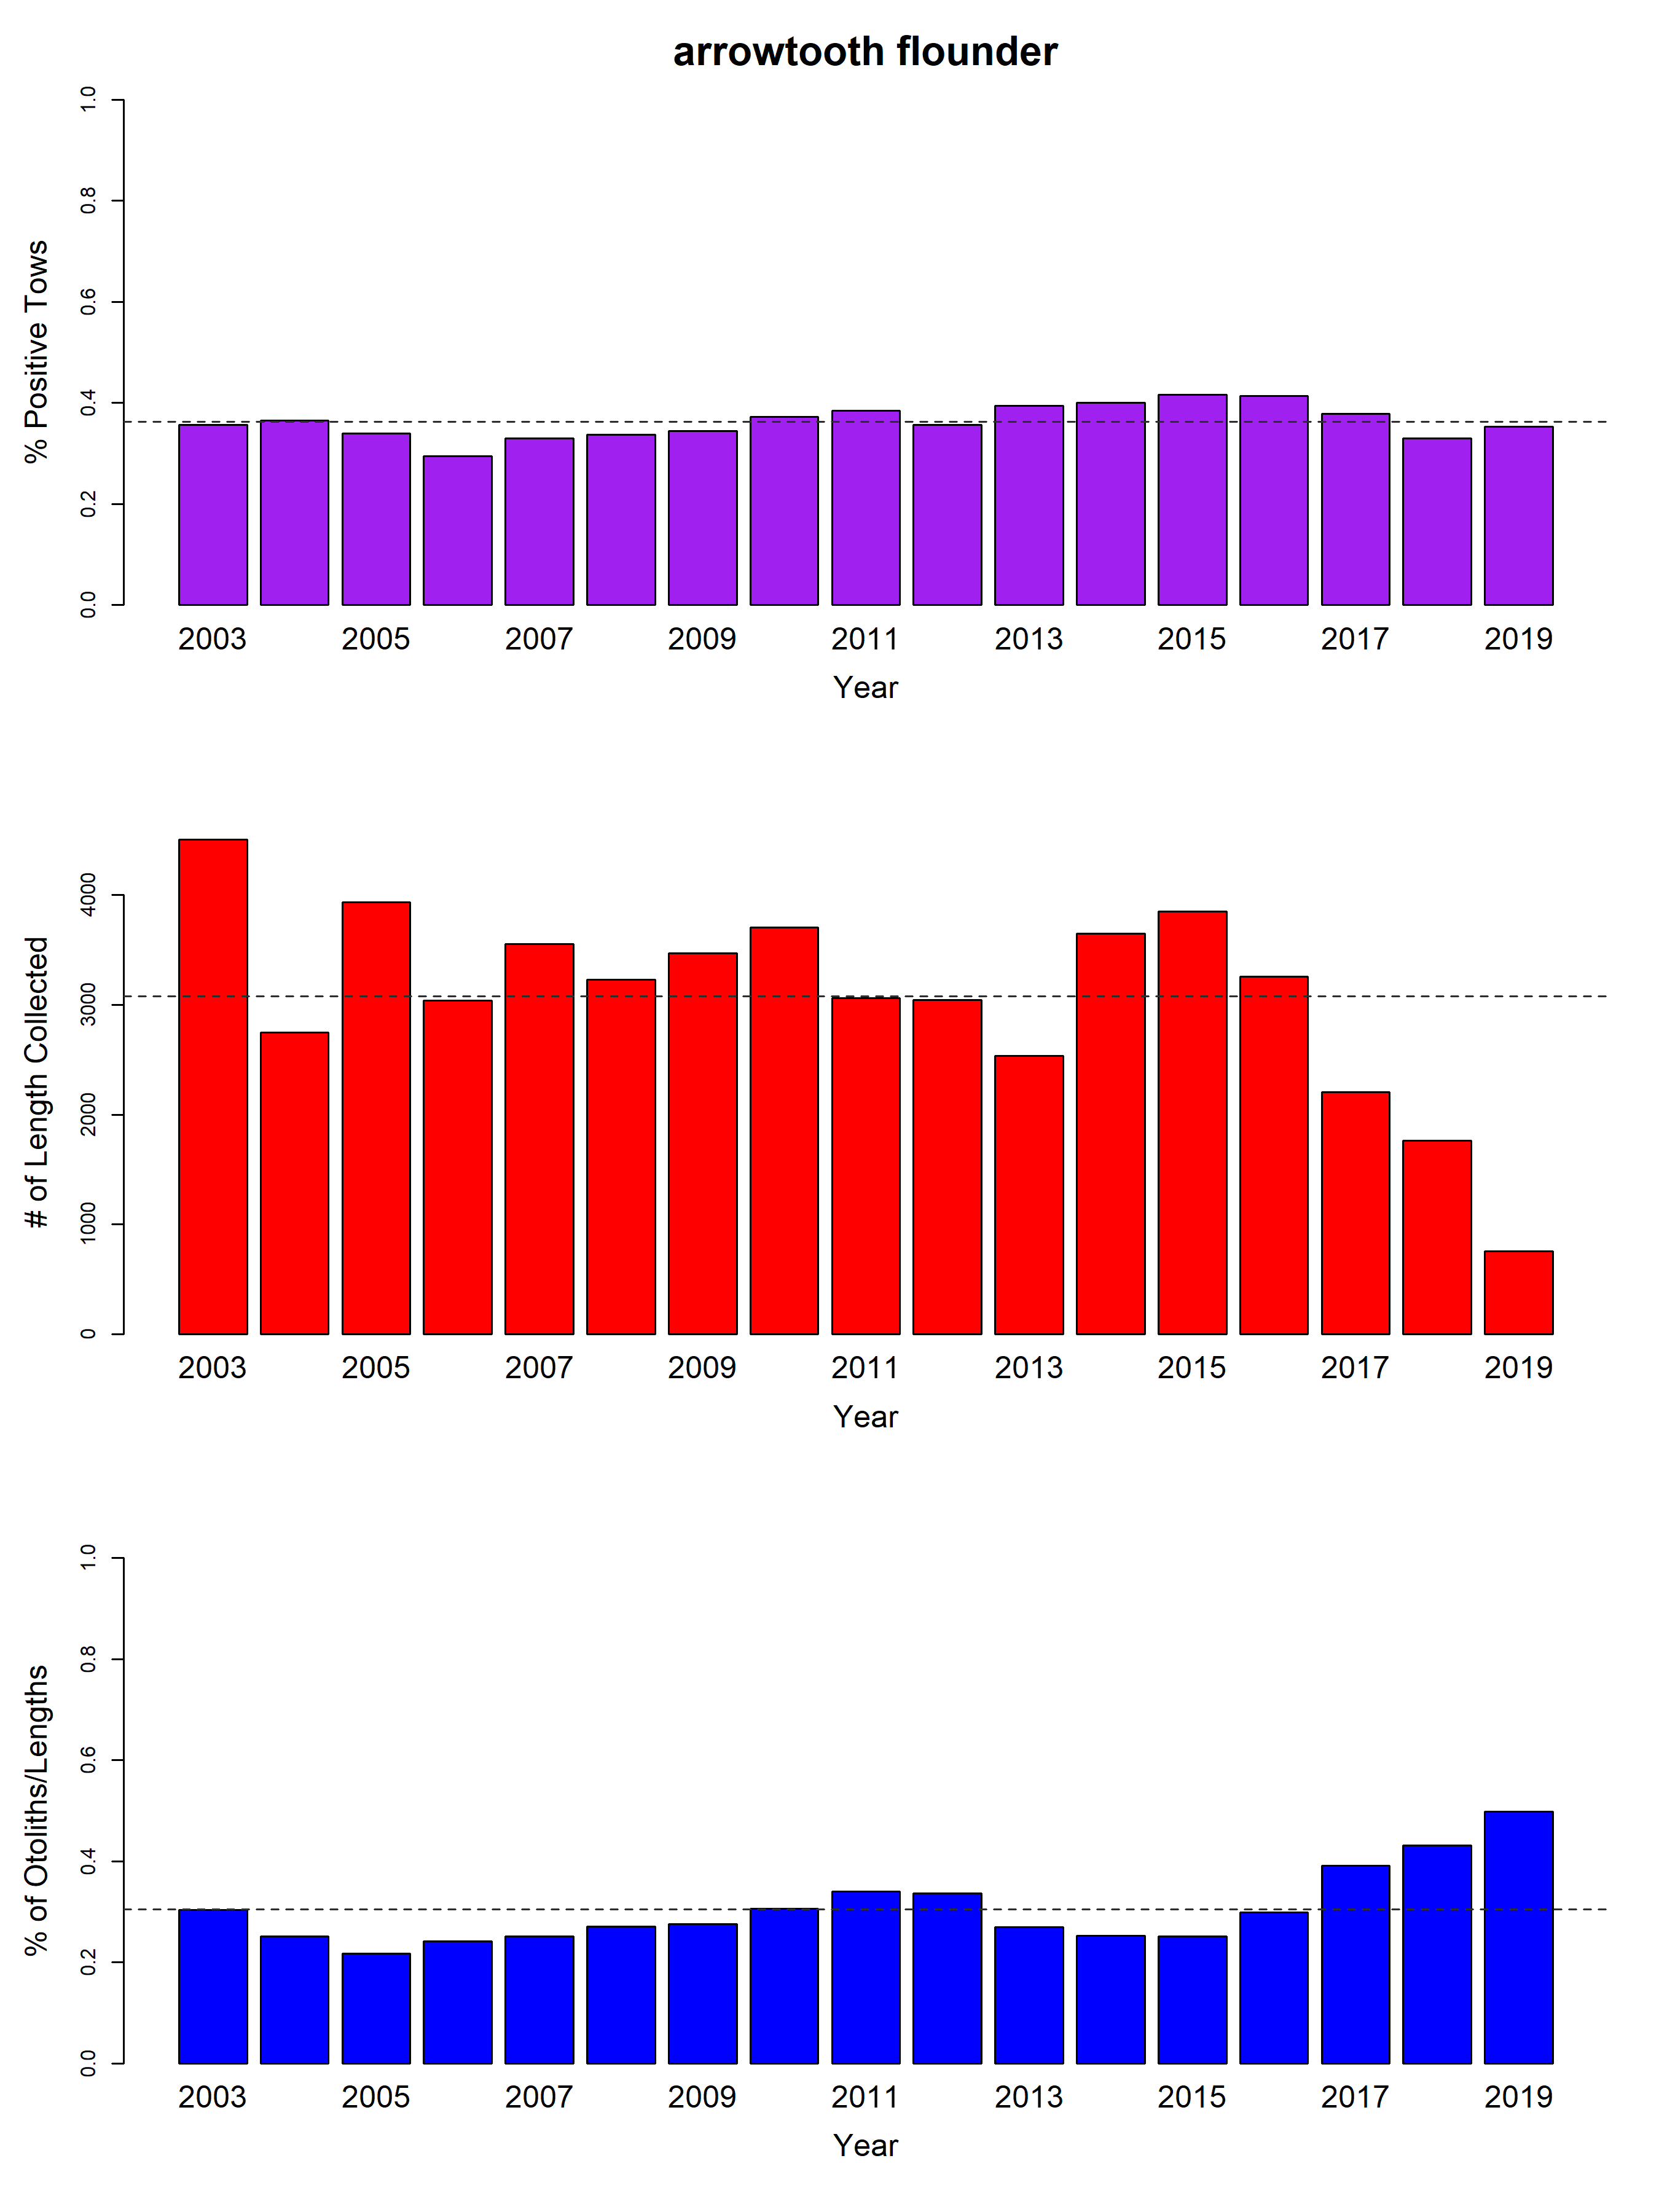
\includegraphics[width=0.6\textwidth,height=\textheight]{C:/Assessments/2020/survey_summary/sum_plots/arrowtooth_flounder_survey_stats.png}
\caption{Summary of collected data for Arrowtooth flounder from the
NWFSC WCGBT survey from 2003 -
2019.\label{fig:nwfsc_arrowtooth_flounder_sum}}
\end{figure}

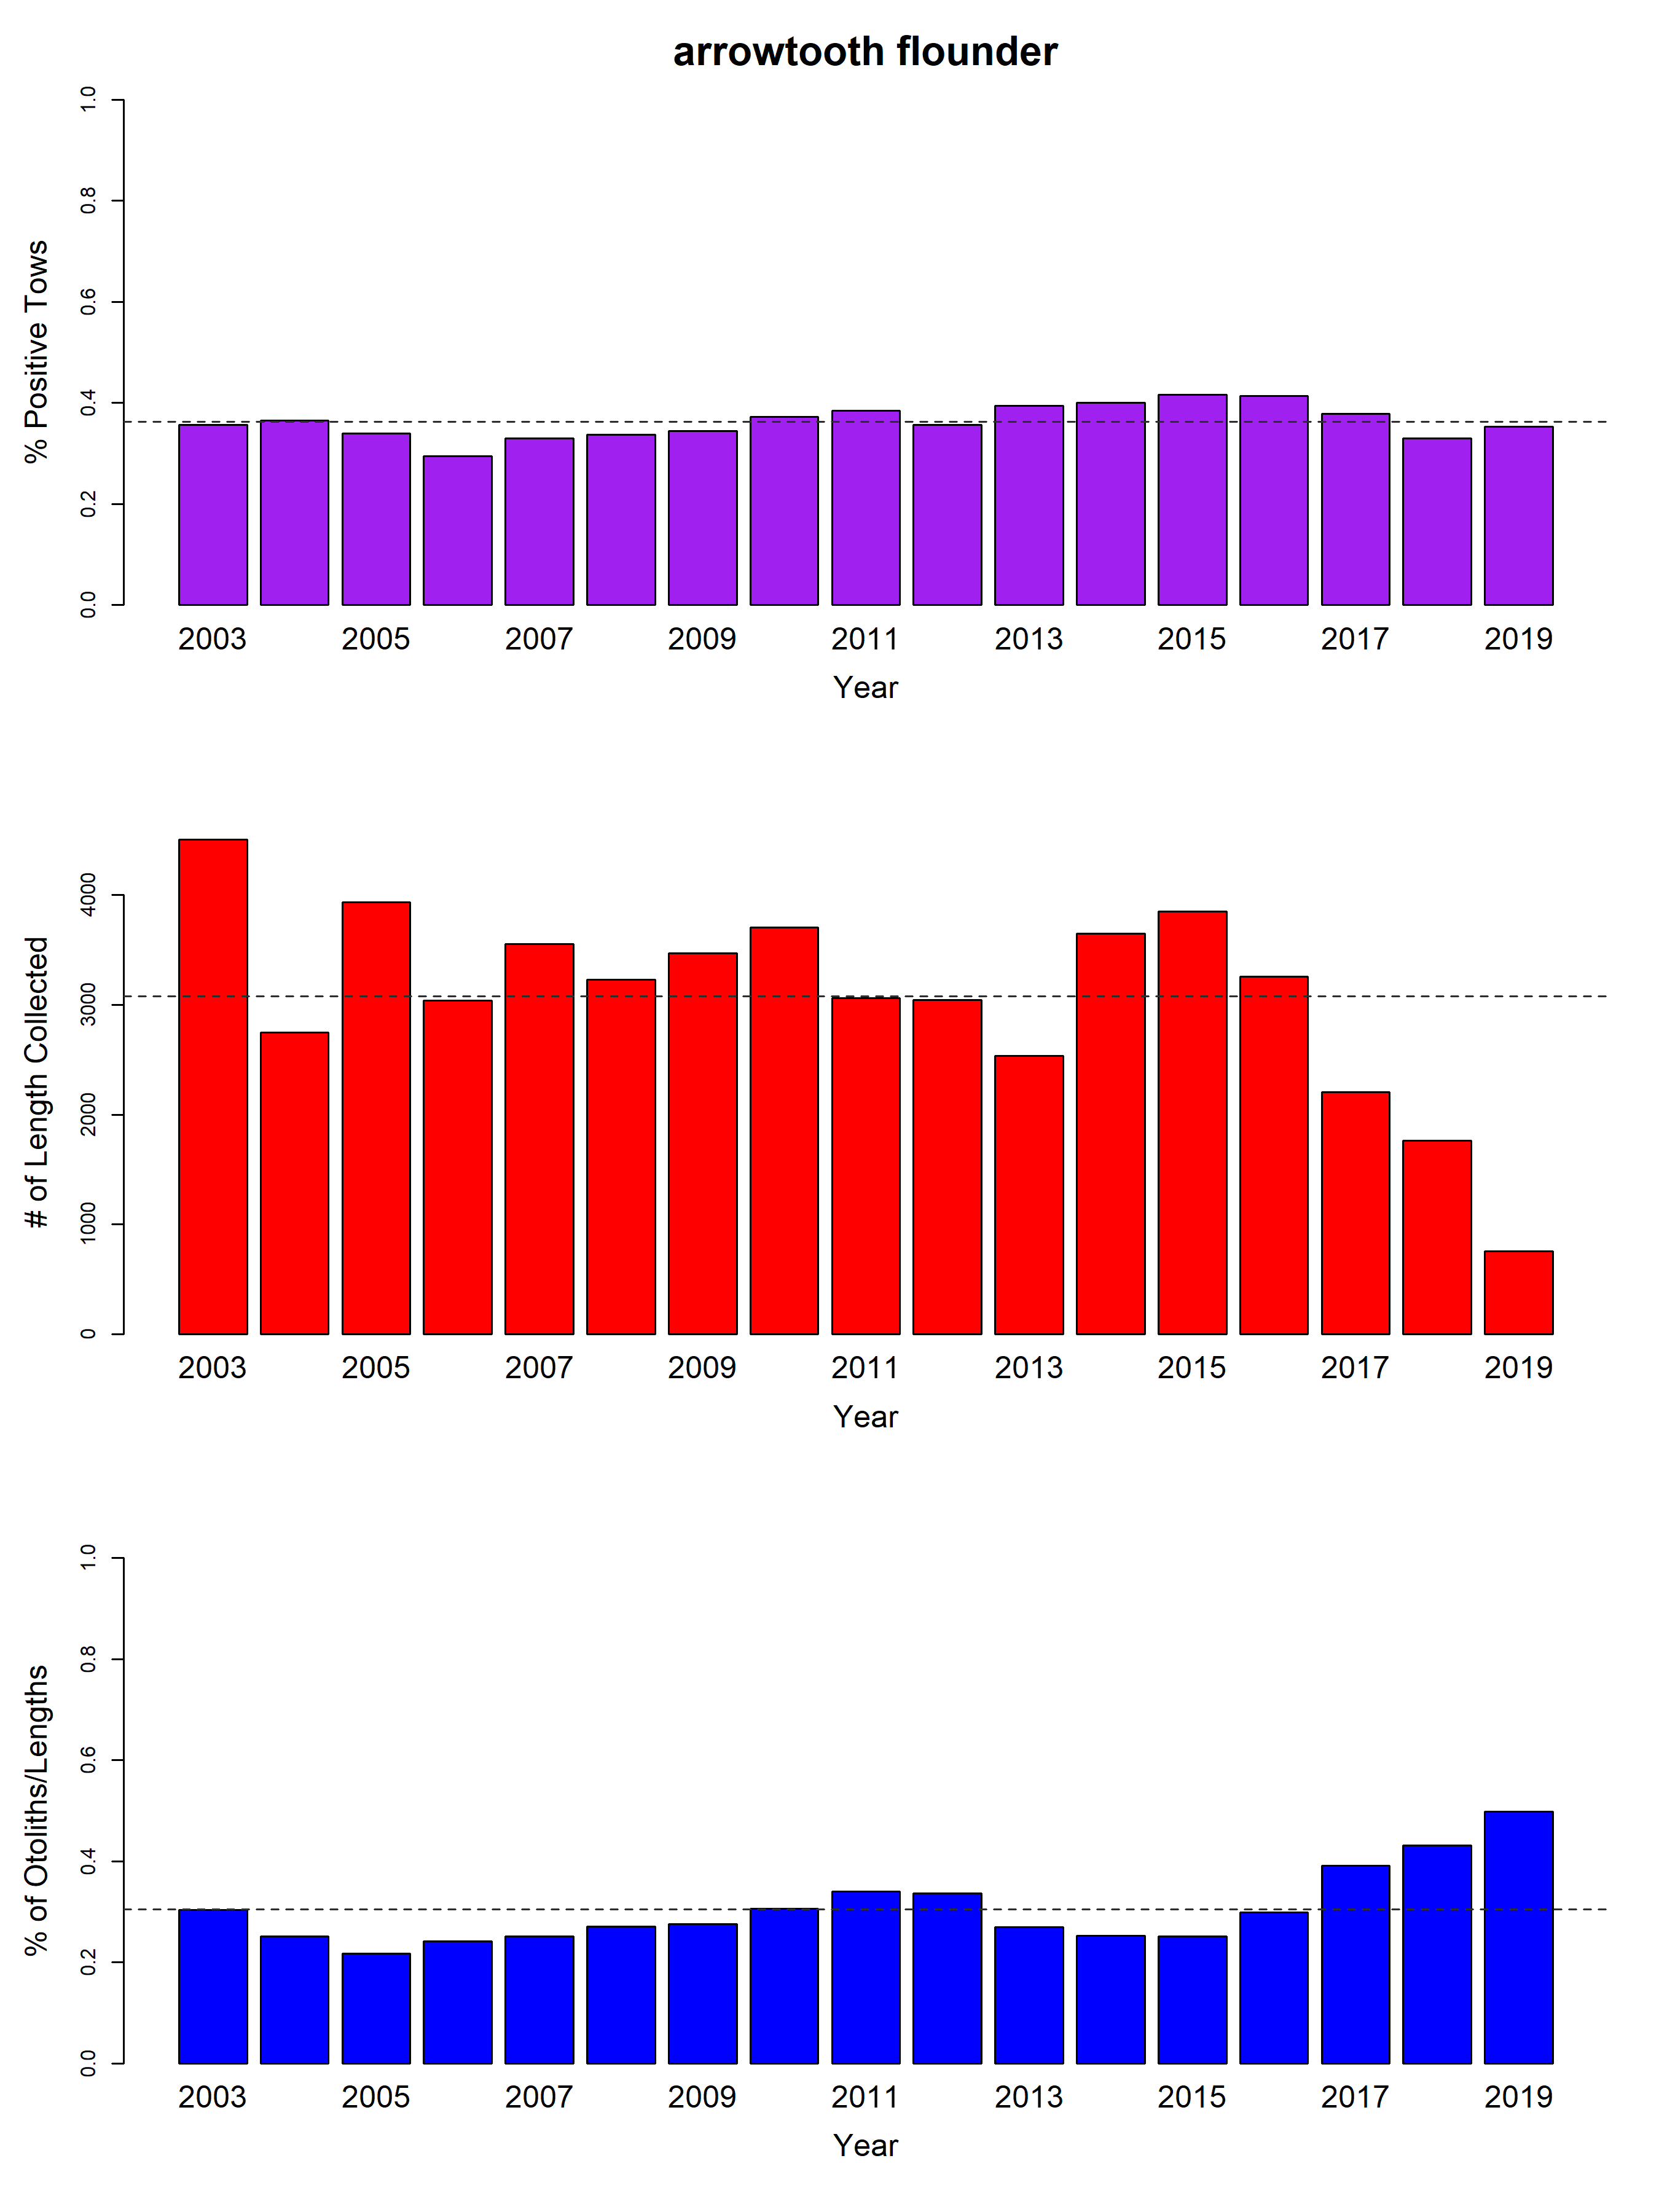
\includegraphics[width=0.6\textwidth,height=\textheight]{C:/Assessments/2020/survey_summary/sum_plots/arrowtooth_flounder_survey_stats.png}
\FloatBarrier  

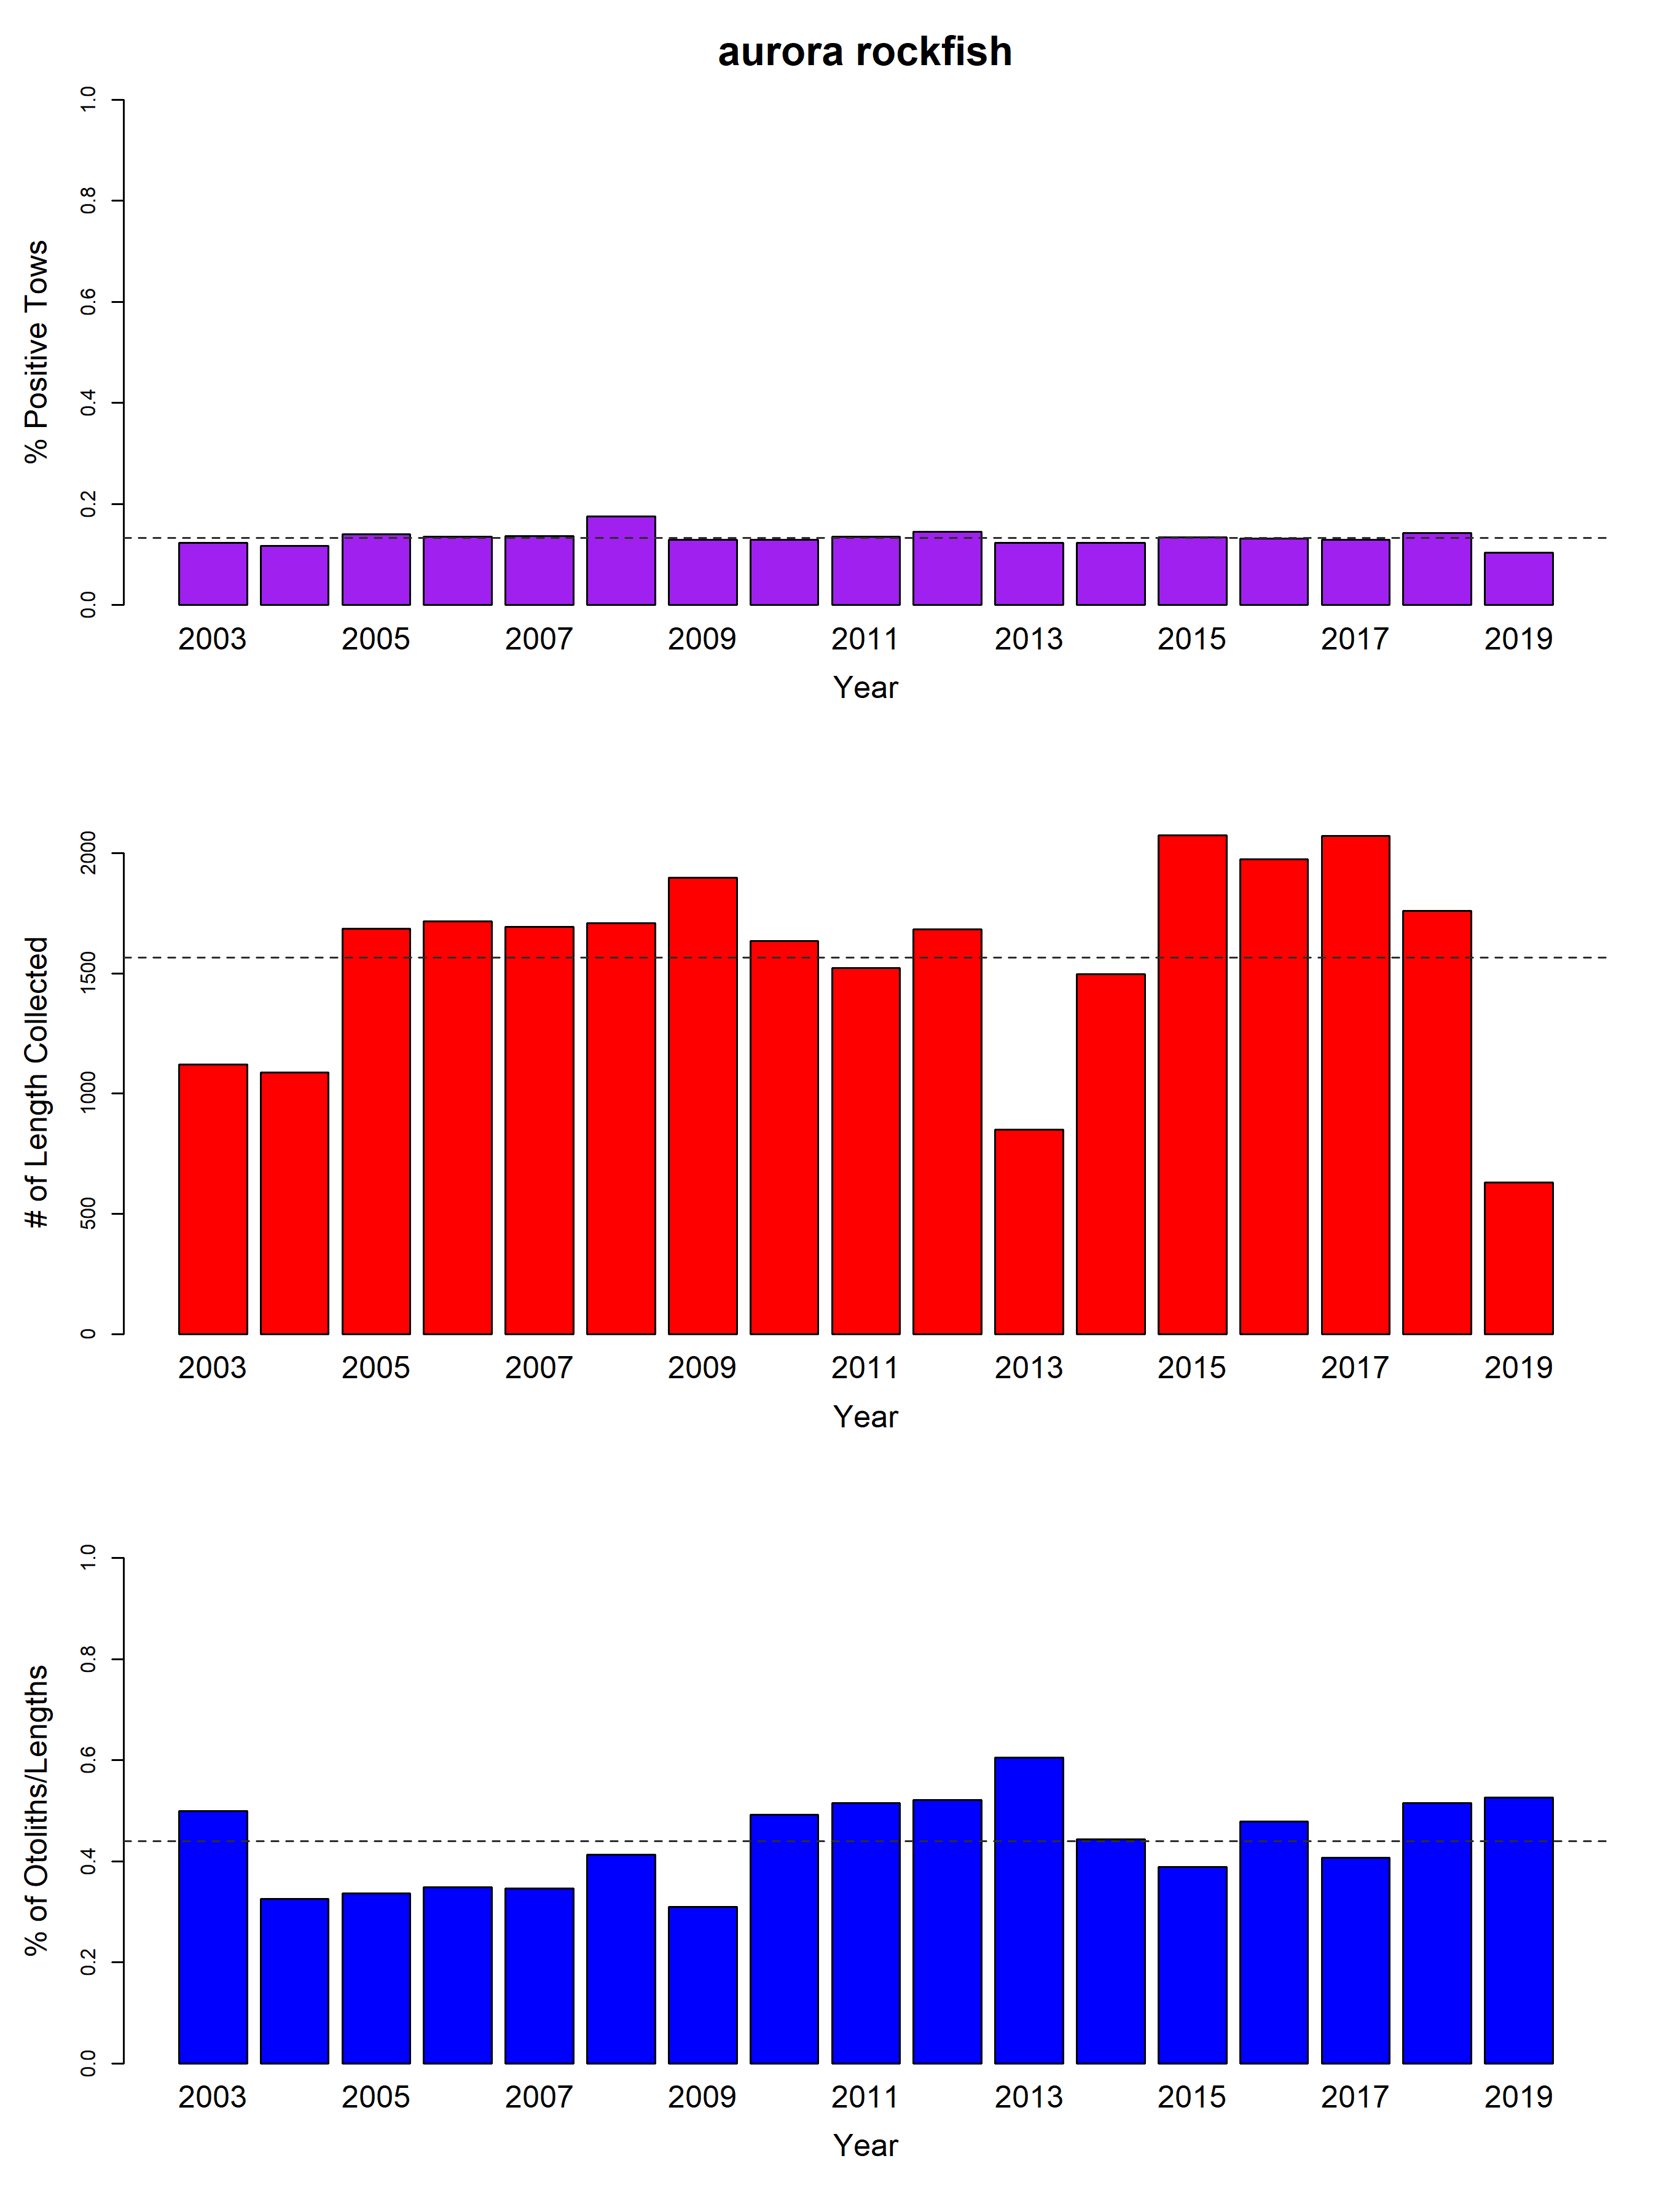
\includegraphics[width=0.6\textwidth,height=\textheight]{C:/Assessments/2020/survey_summary/sum_plots/aurora_rockfish_survey_stats.png}
\FloatBarrier  

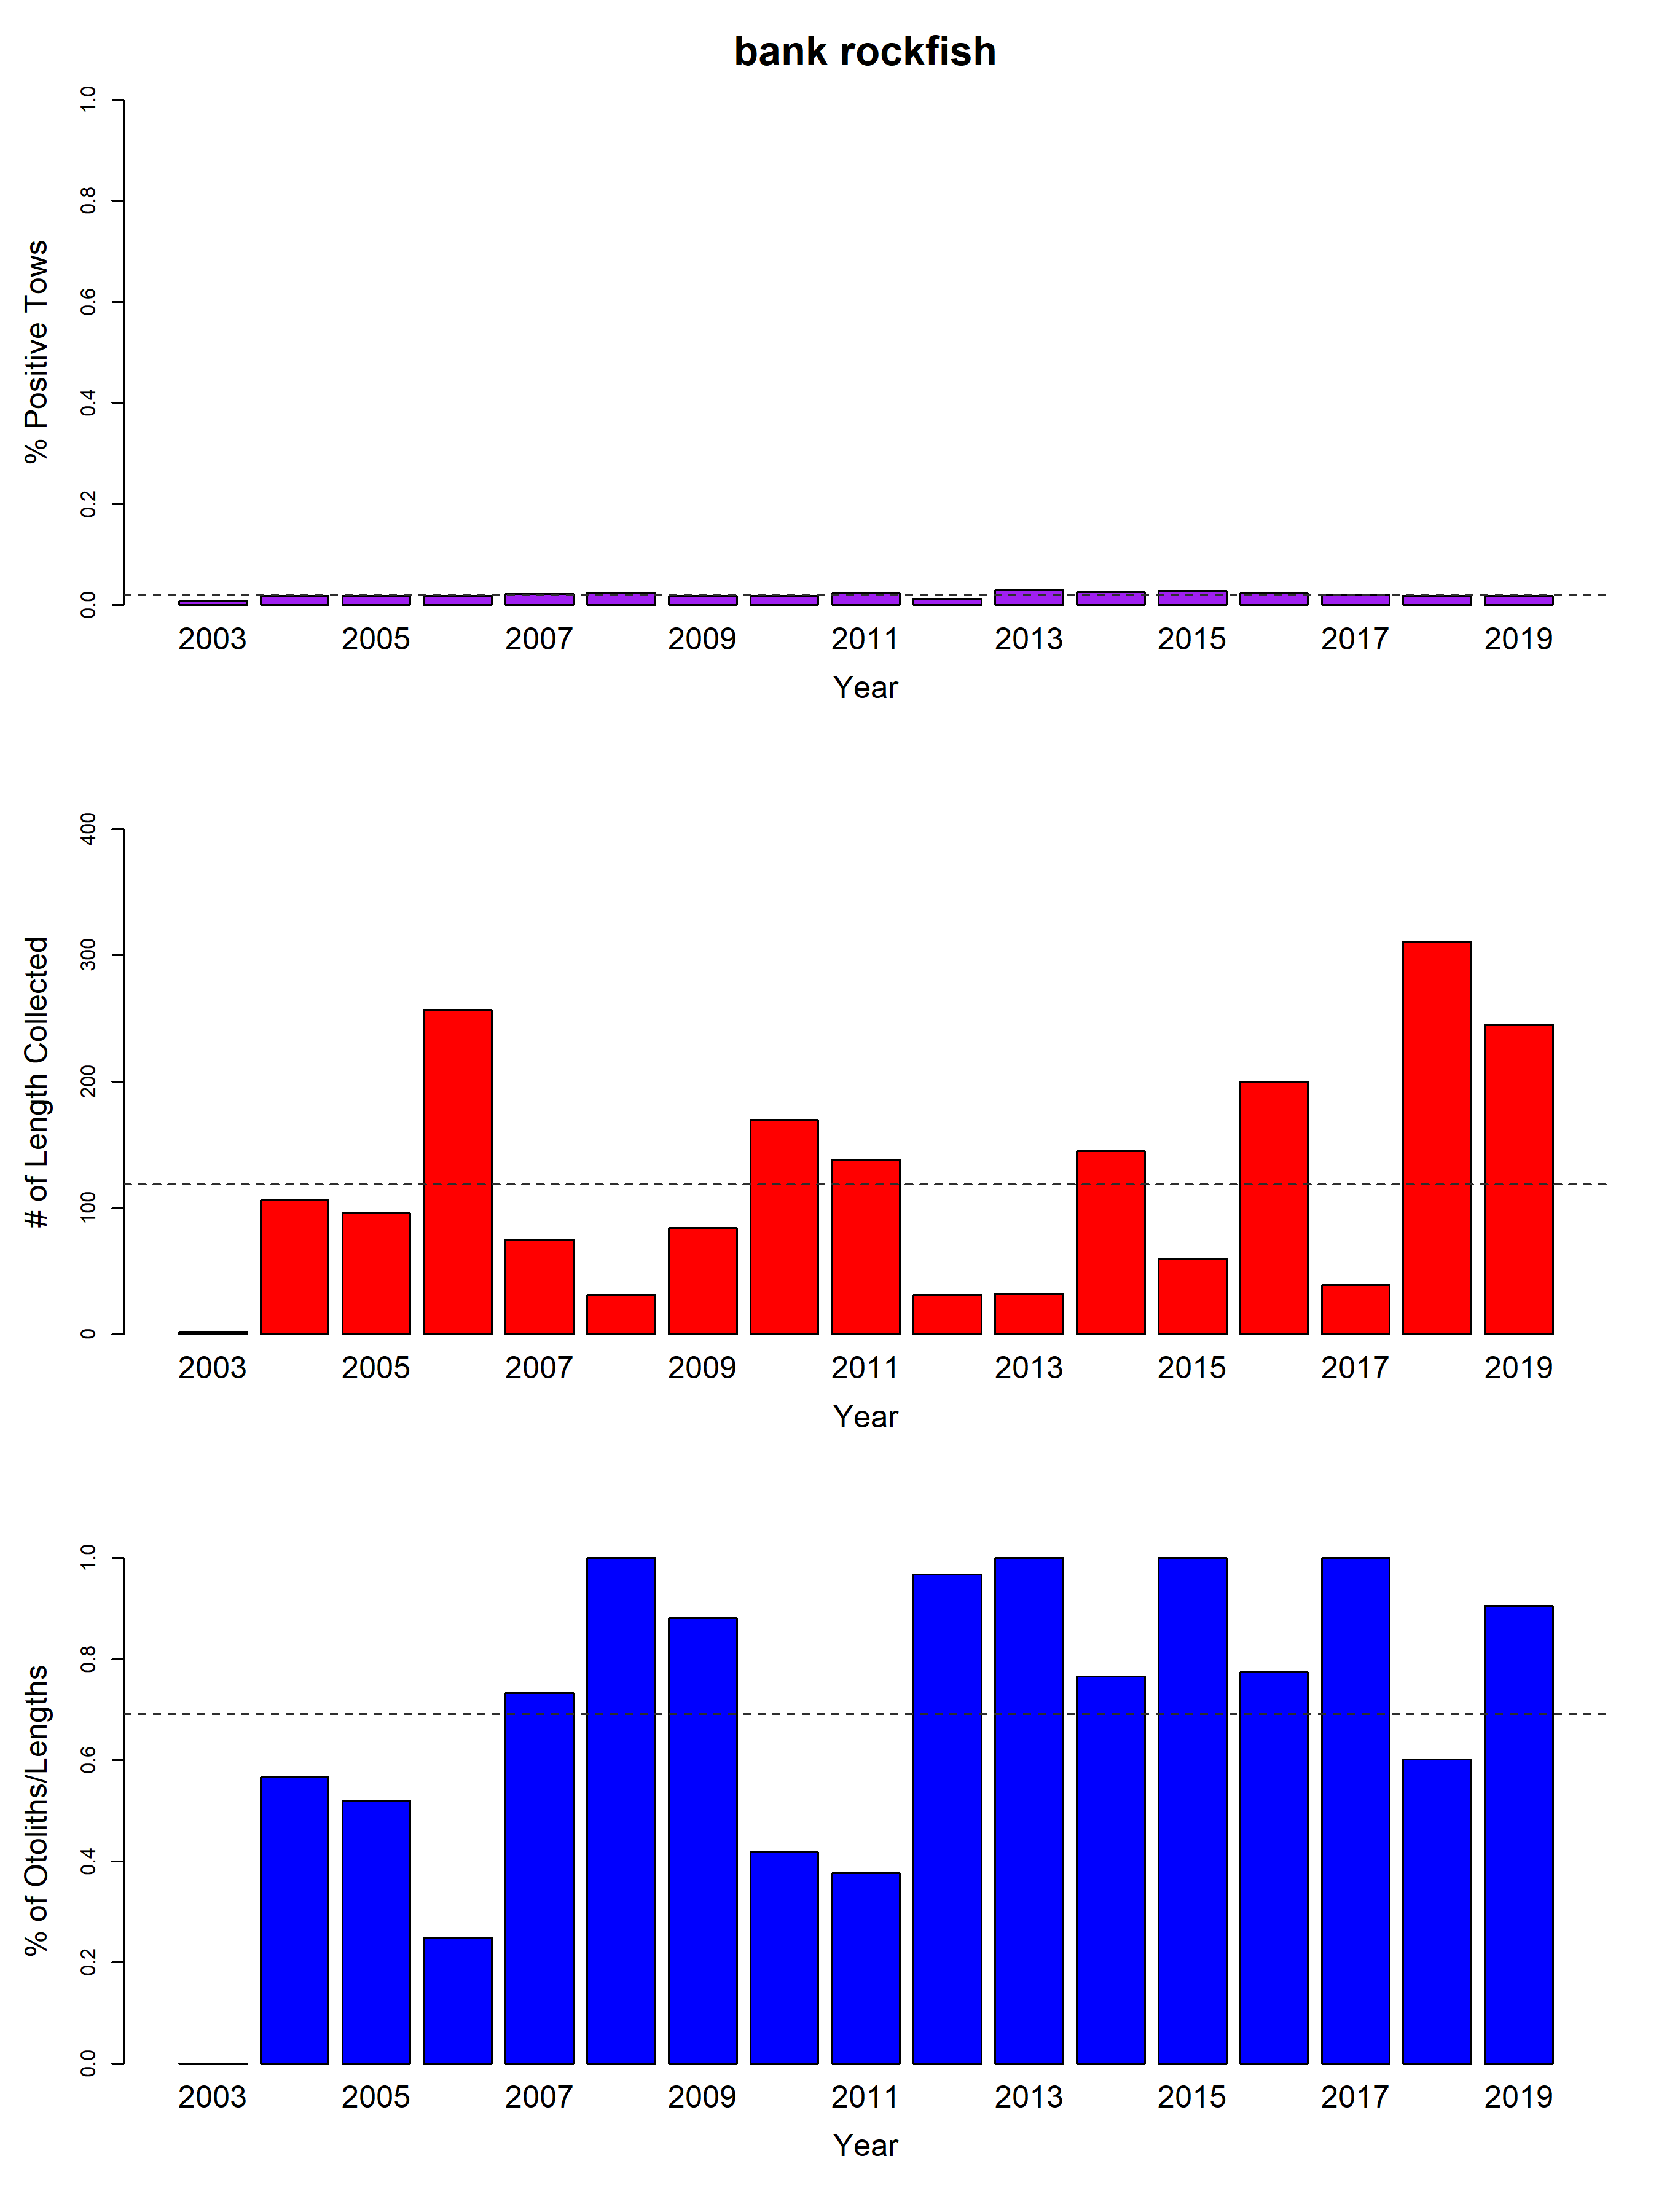
\includegraphics[width=0.6\textwidth,height=\textheight]{C:/Assessments/2020/survey_summary/sum_plots/bank_rockfish_survey_stats.png}
\FloatBarrier  

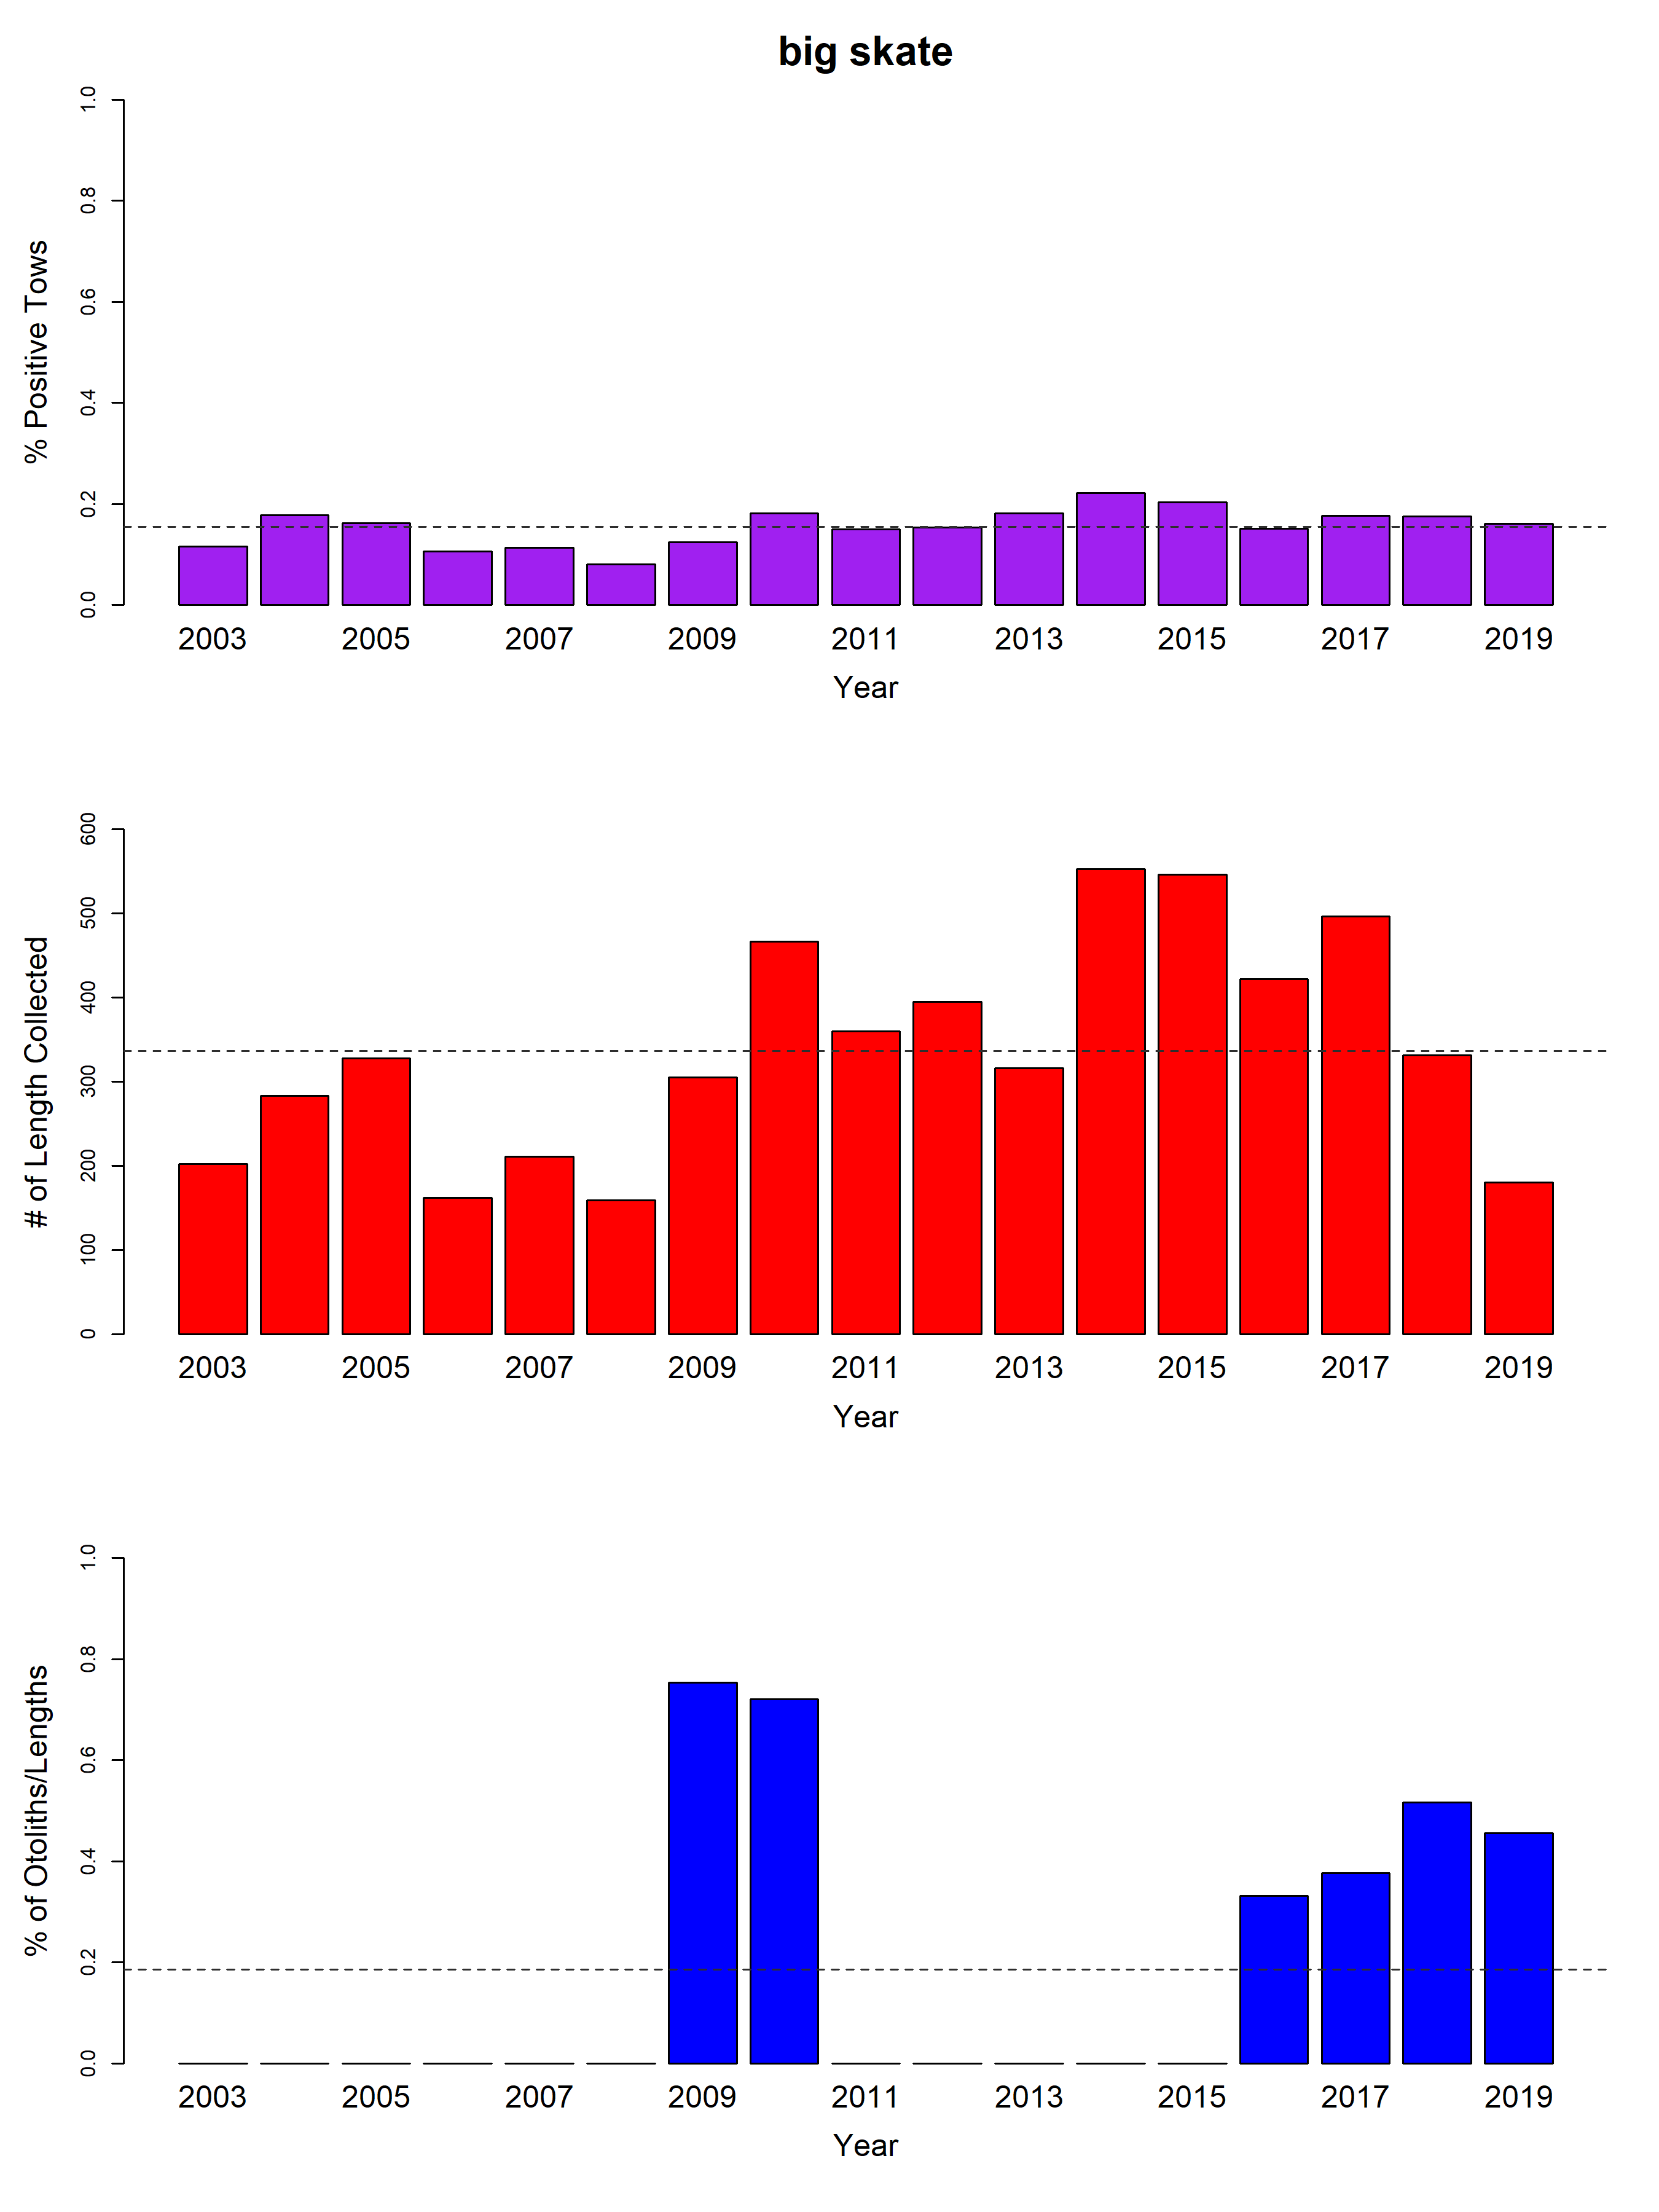
\includegraphics[width=0.6\textwidth,height=\textheight]{C:/Assessments/2020/survey_summary/sum_plots/big_skate_survey_stats.png}
\FloatBarrier  

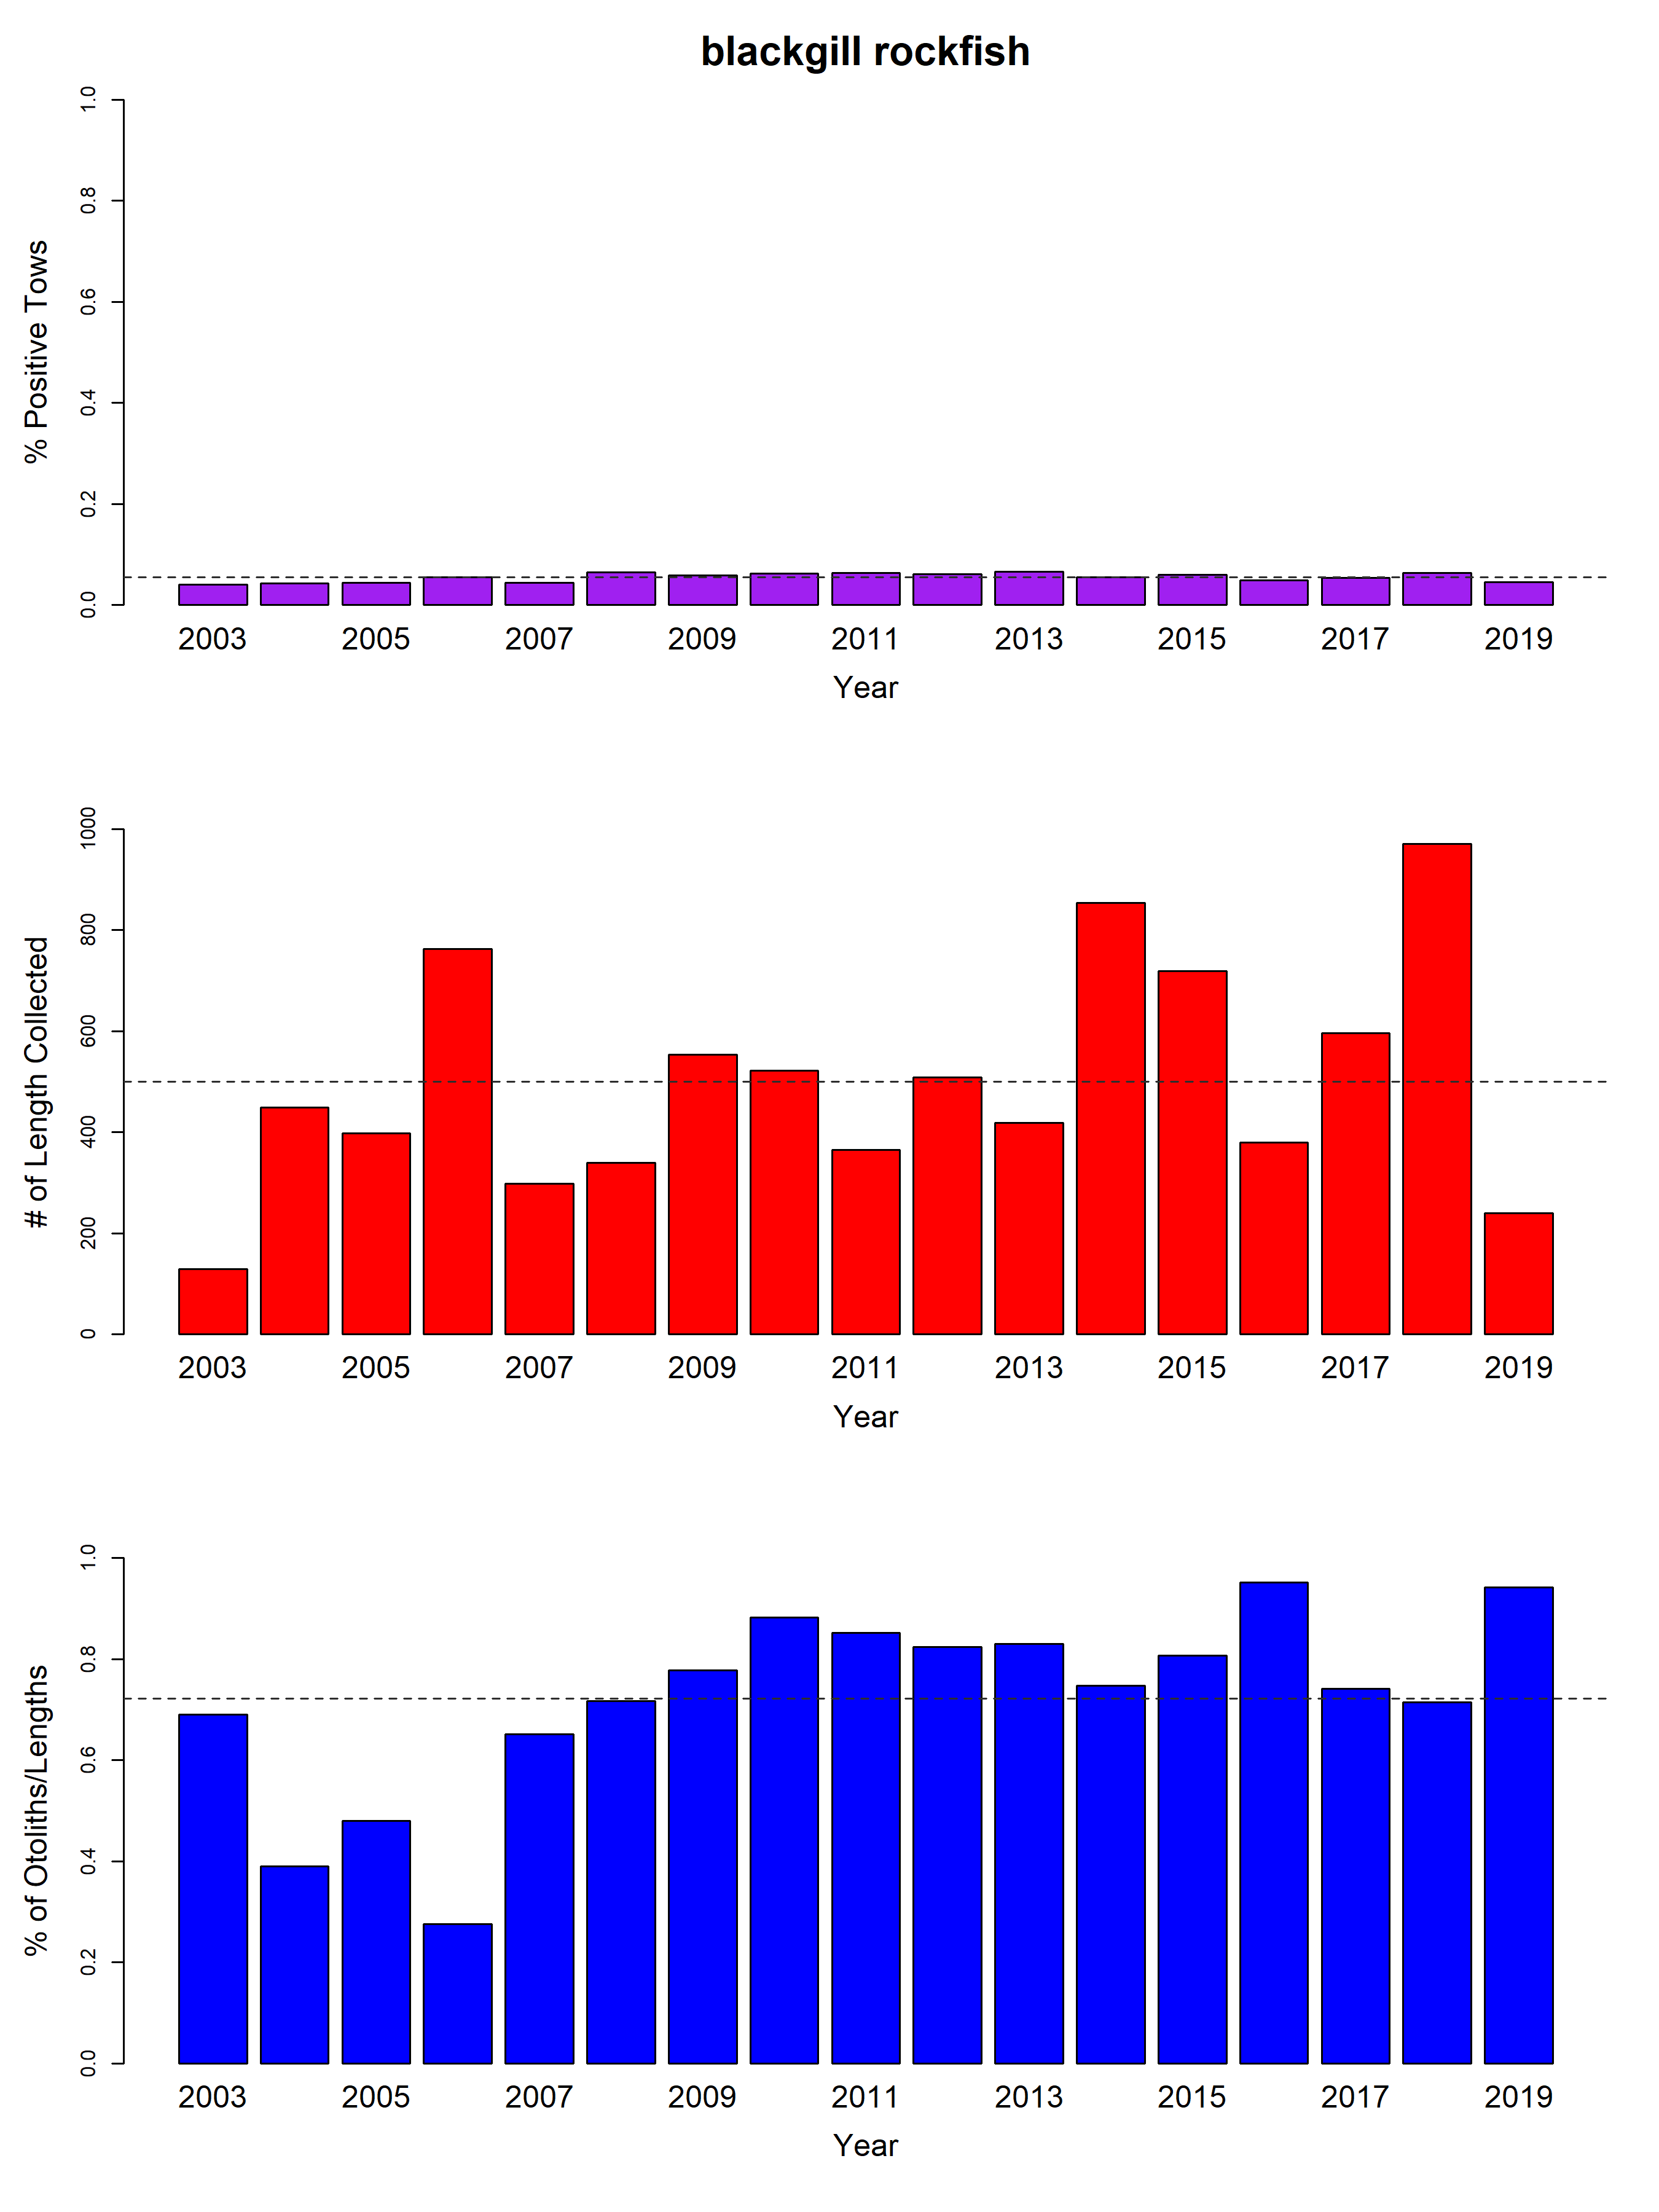
\includegraphics[width=0.6\textwidth,height=\textheight]{C:/Assessments/2020/survey_summary/sum_plots/blackgill_rockfish_survey_stats.png}
\FloatBarrier  

\FloatBarrier

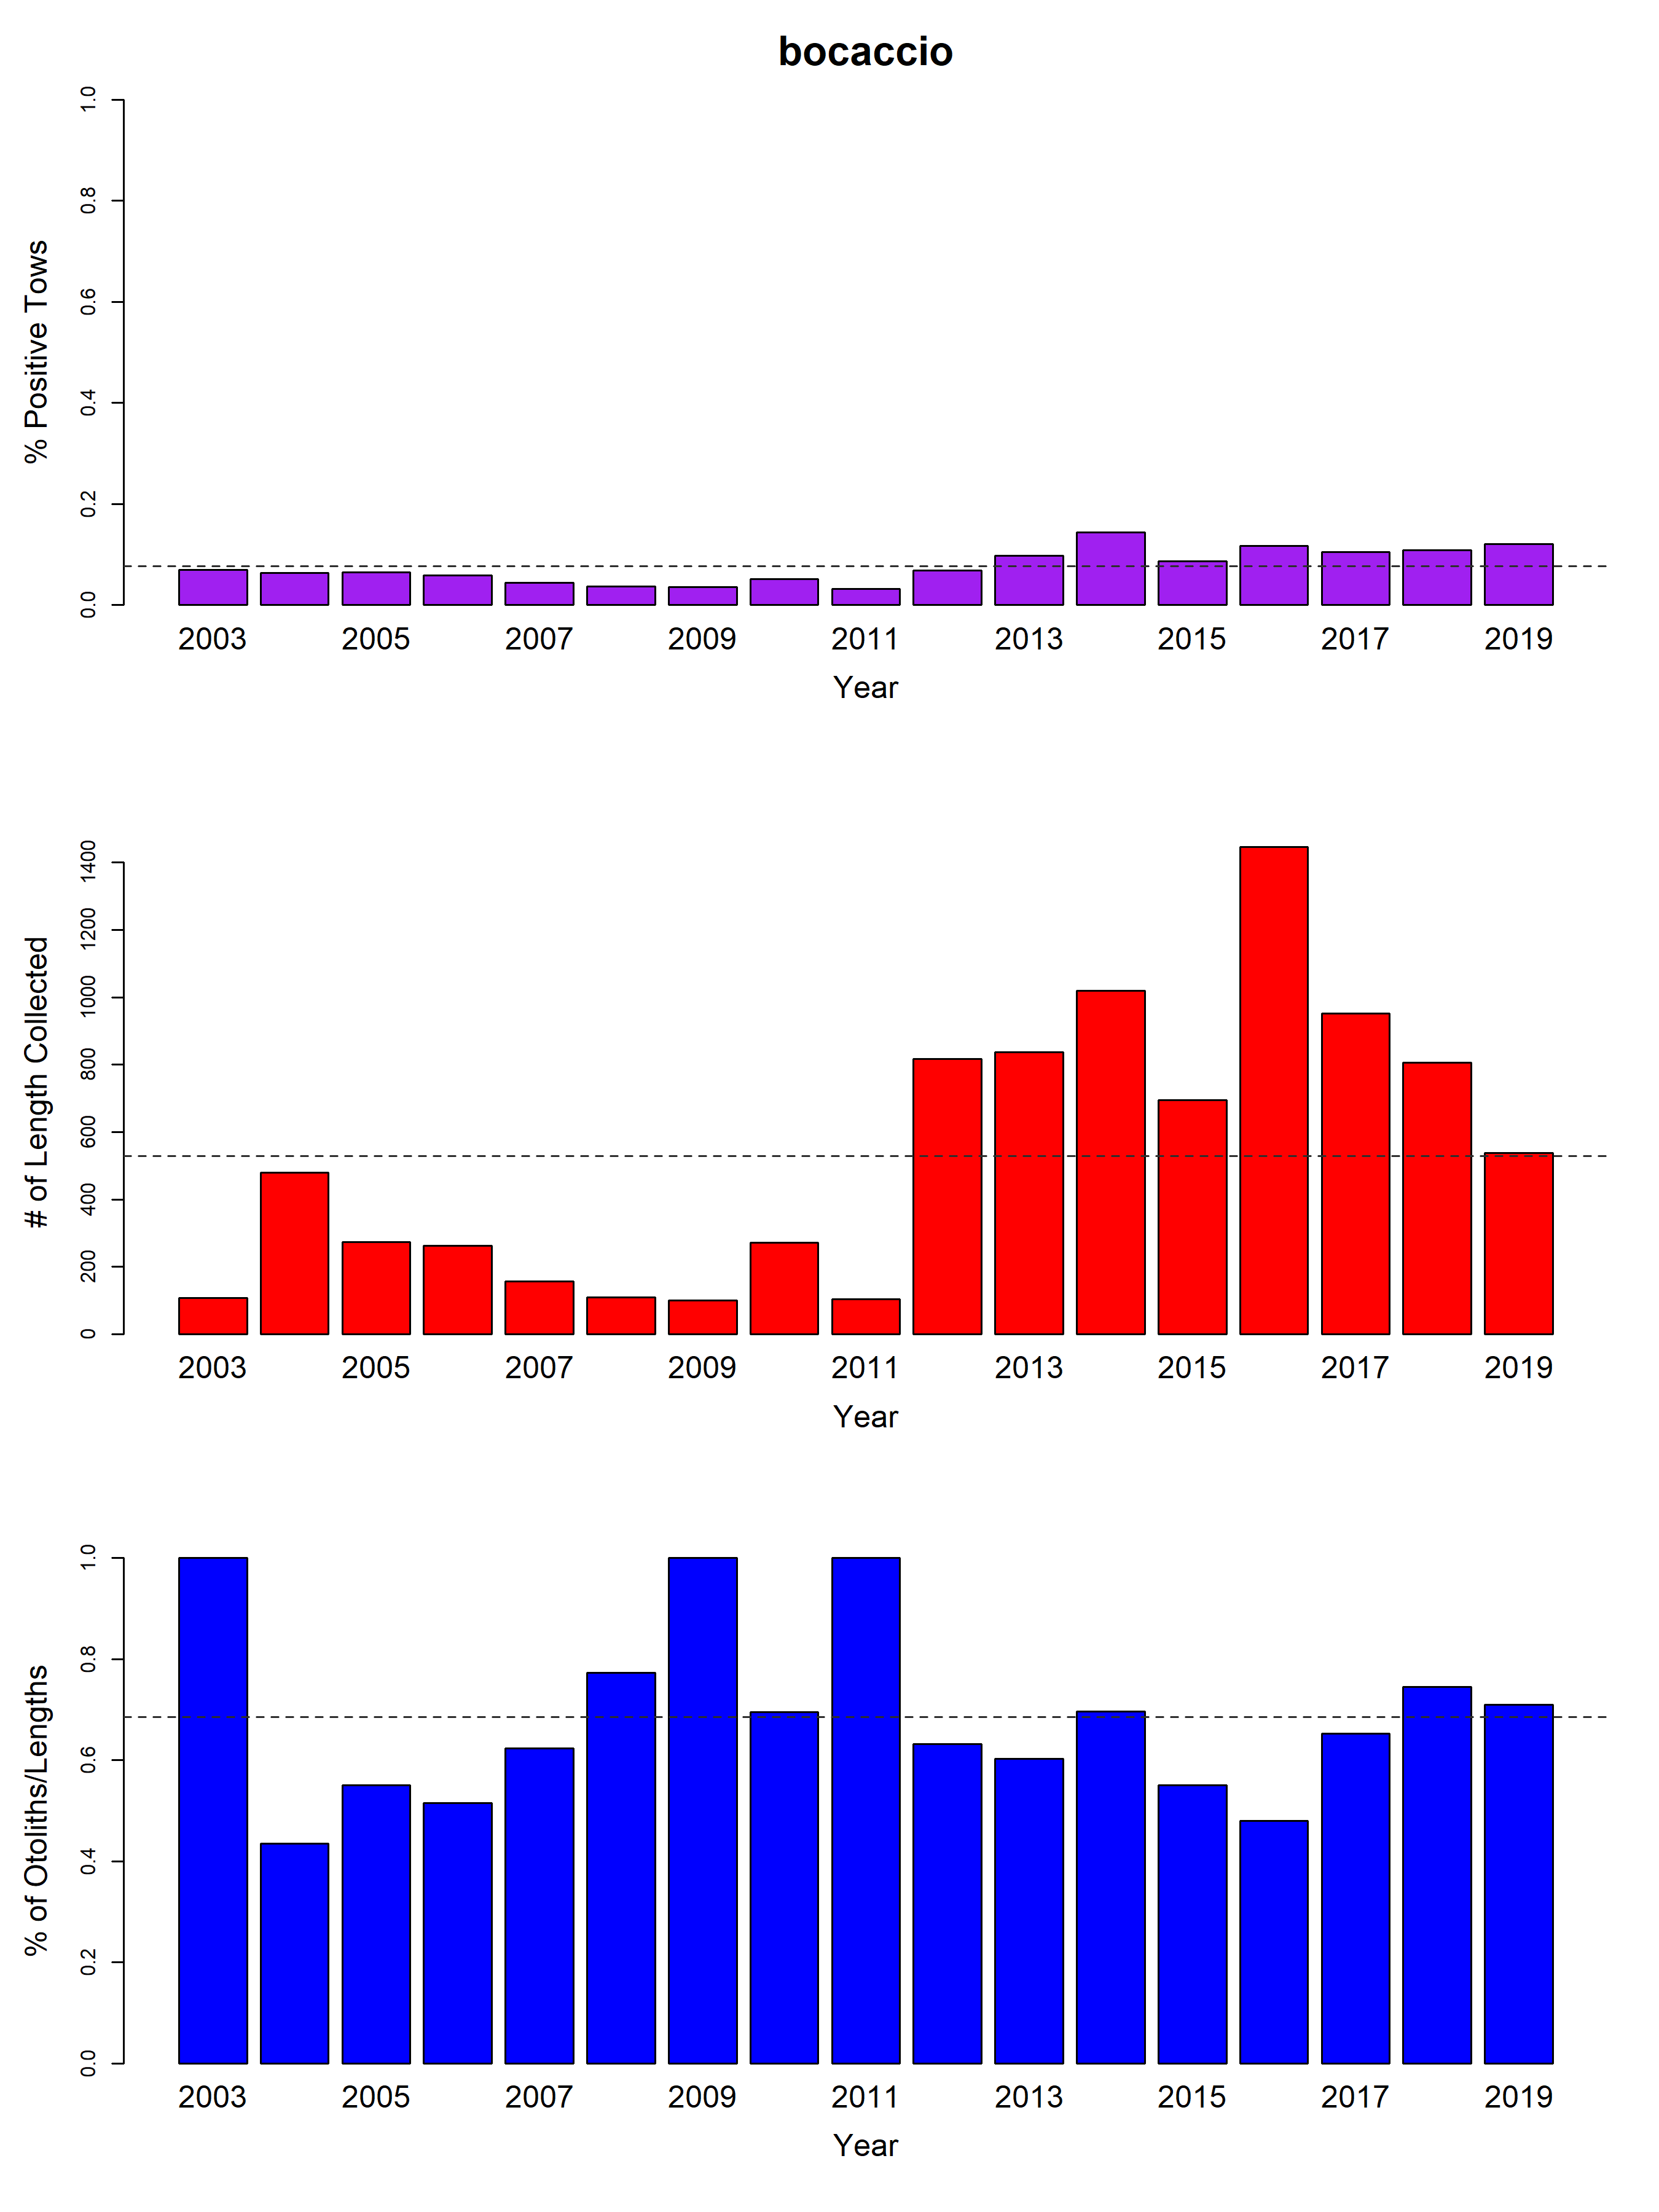
\includegraphics[width=0.6\textwidth,height=\textheight]{C:/Assessments/2020/survey_summary/sum_plots/bocaccio_survey_stats.png}
\FloatBarrier  

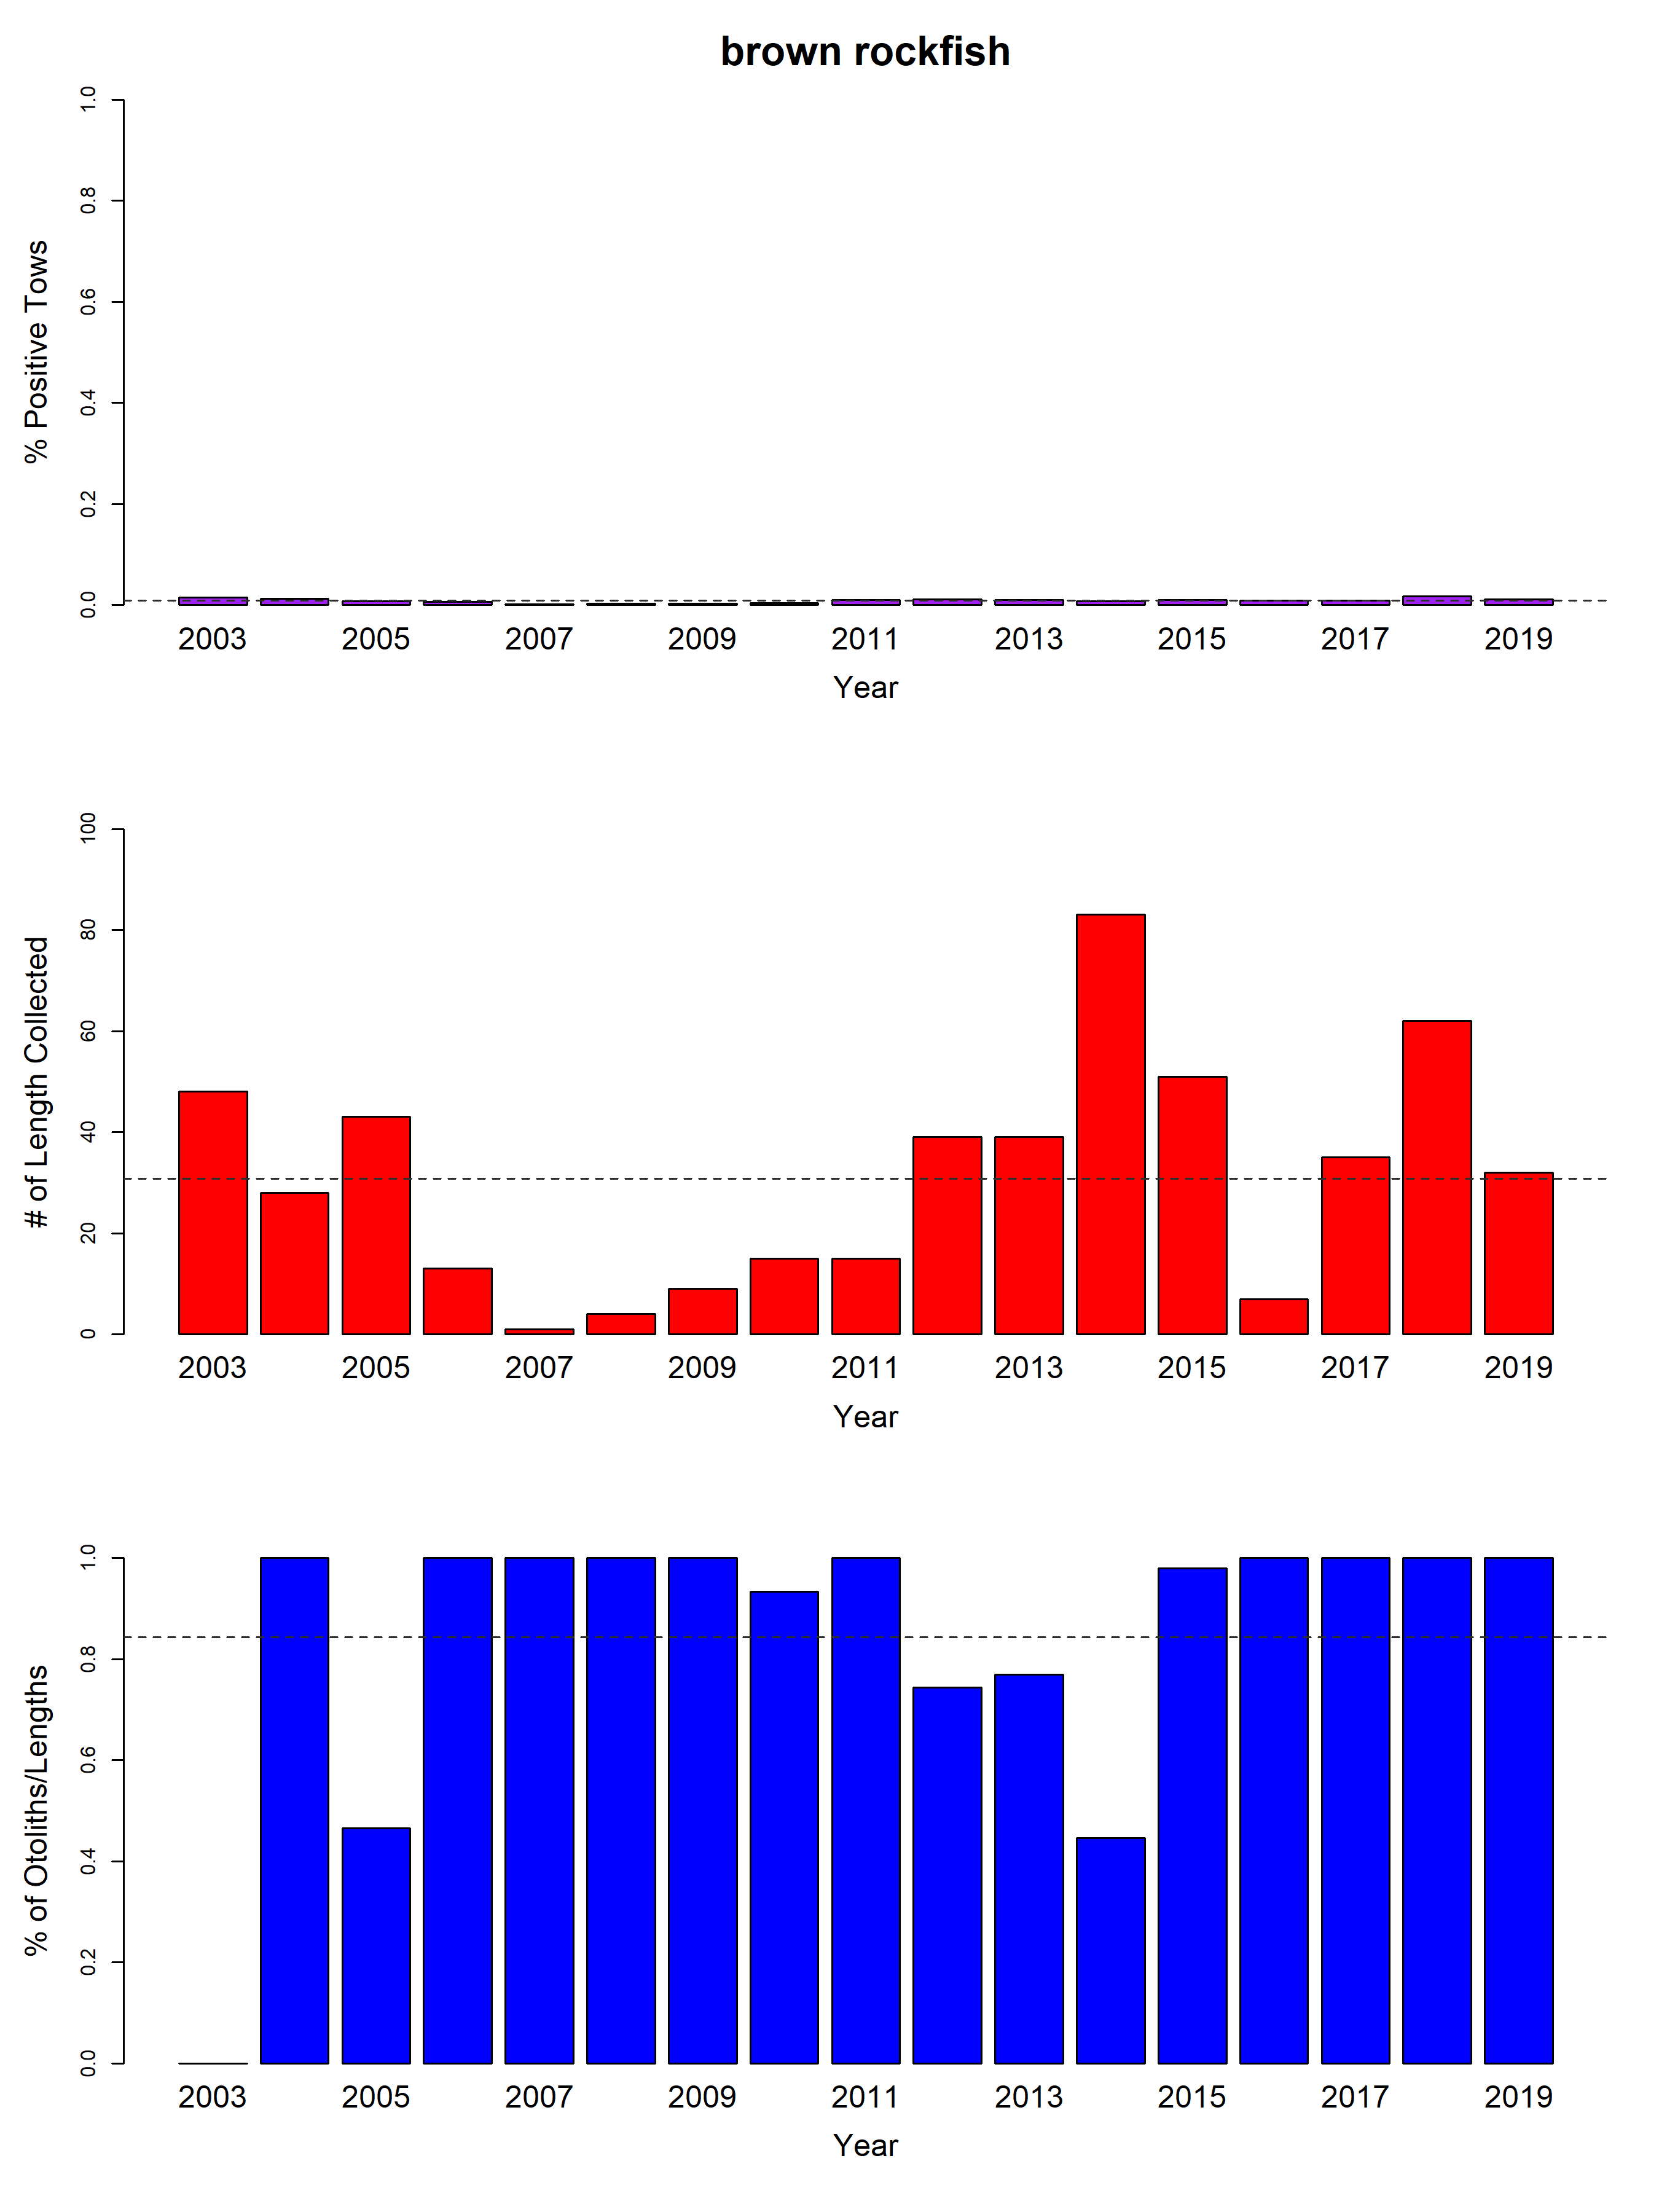
\includegraphics[width=0.6\textwidth,height=\textheight]{C:/Assessments/2020/survey_summary/sum_plots/brown_rockfish_survey_stats.png}
\FloatBarrier  

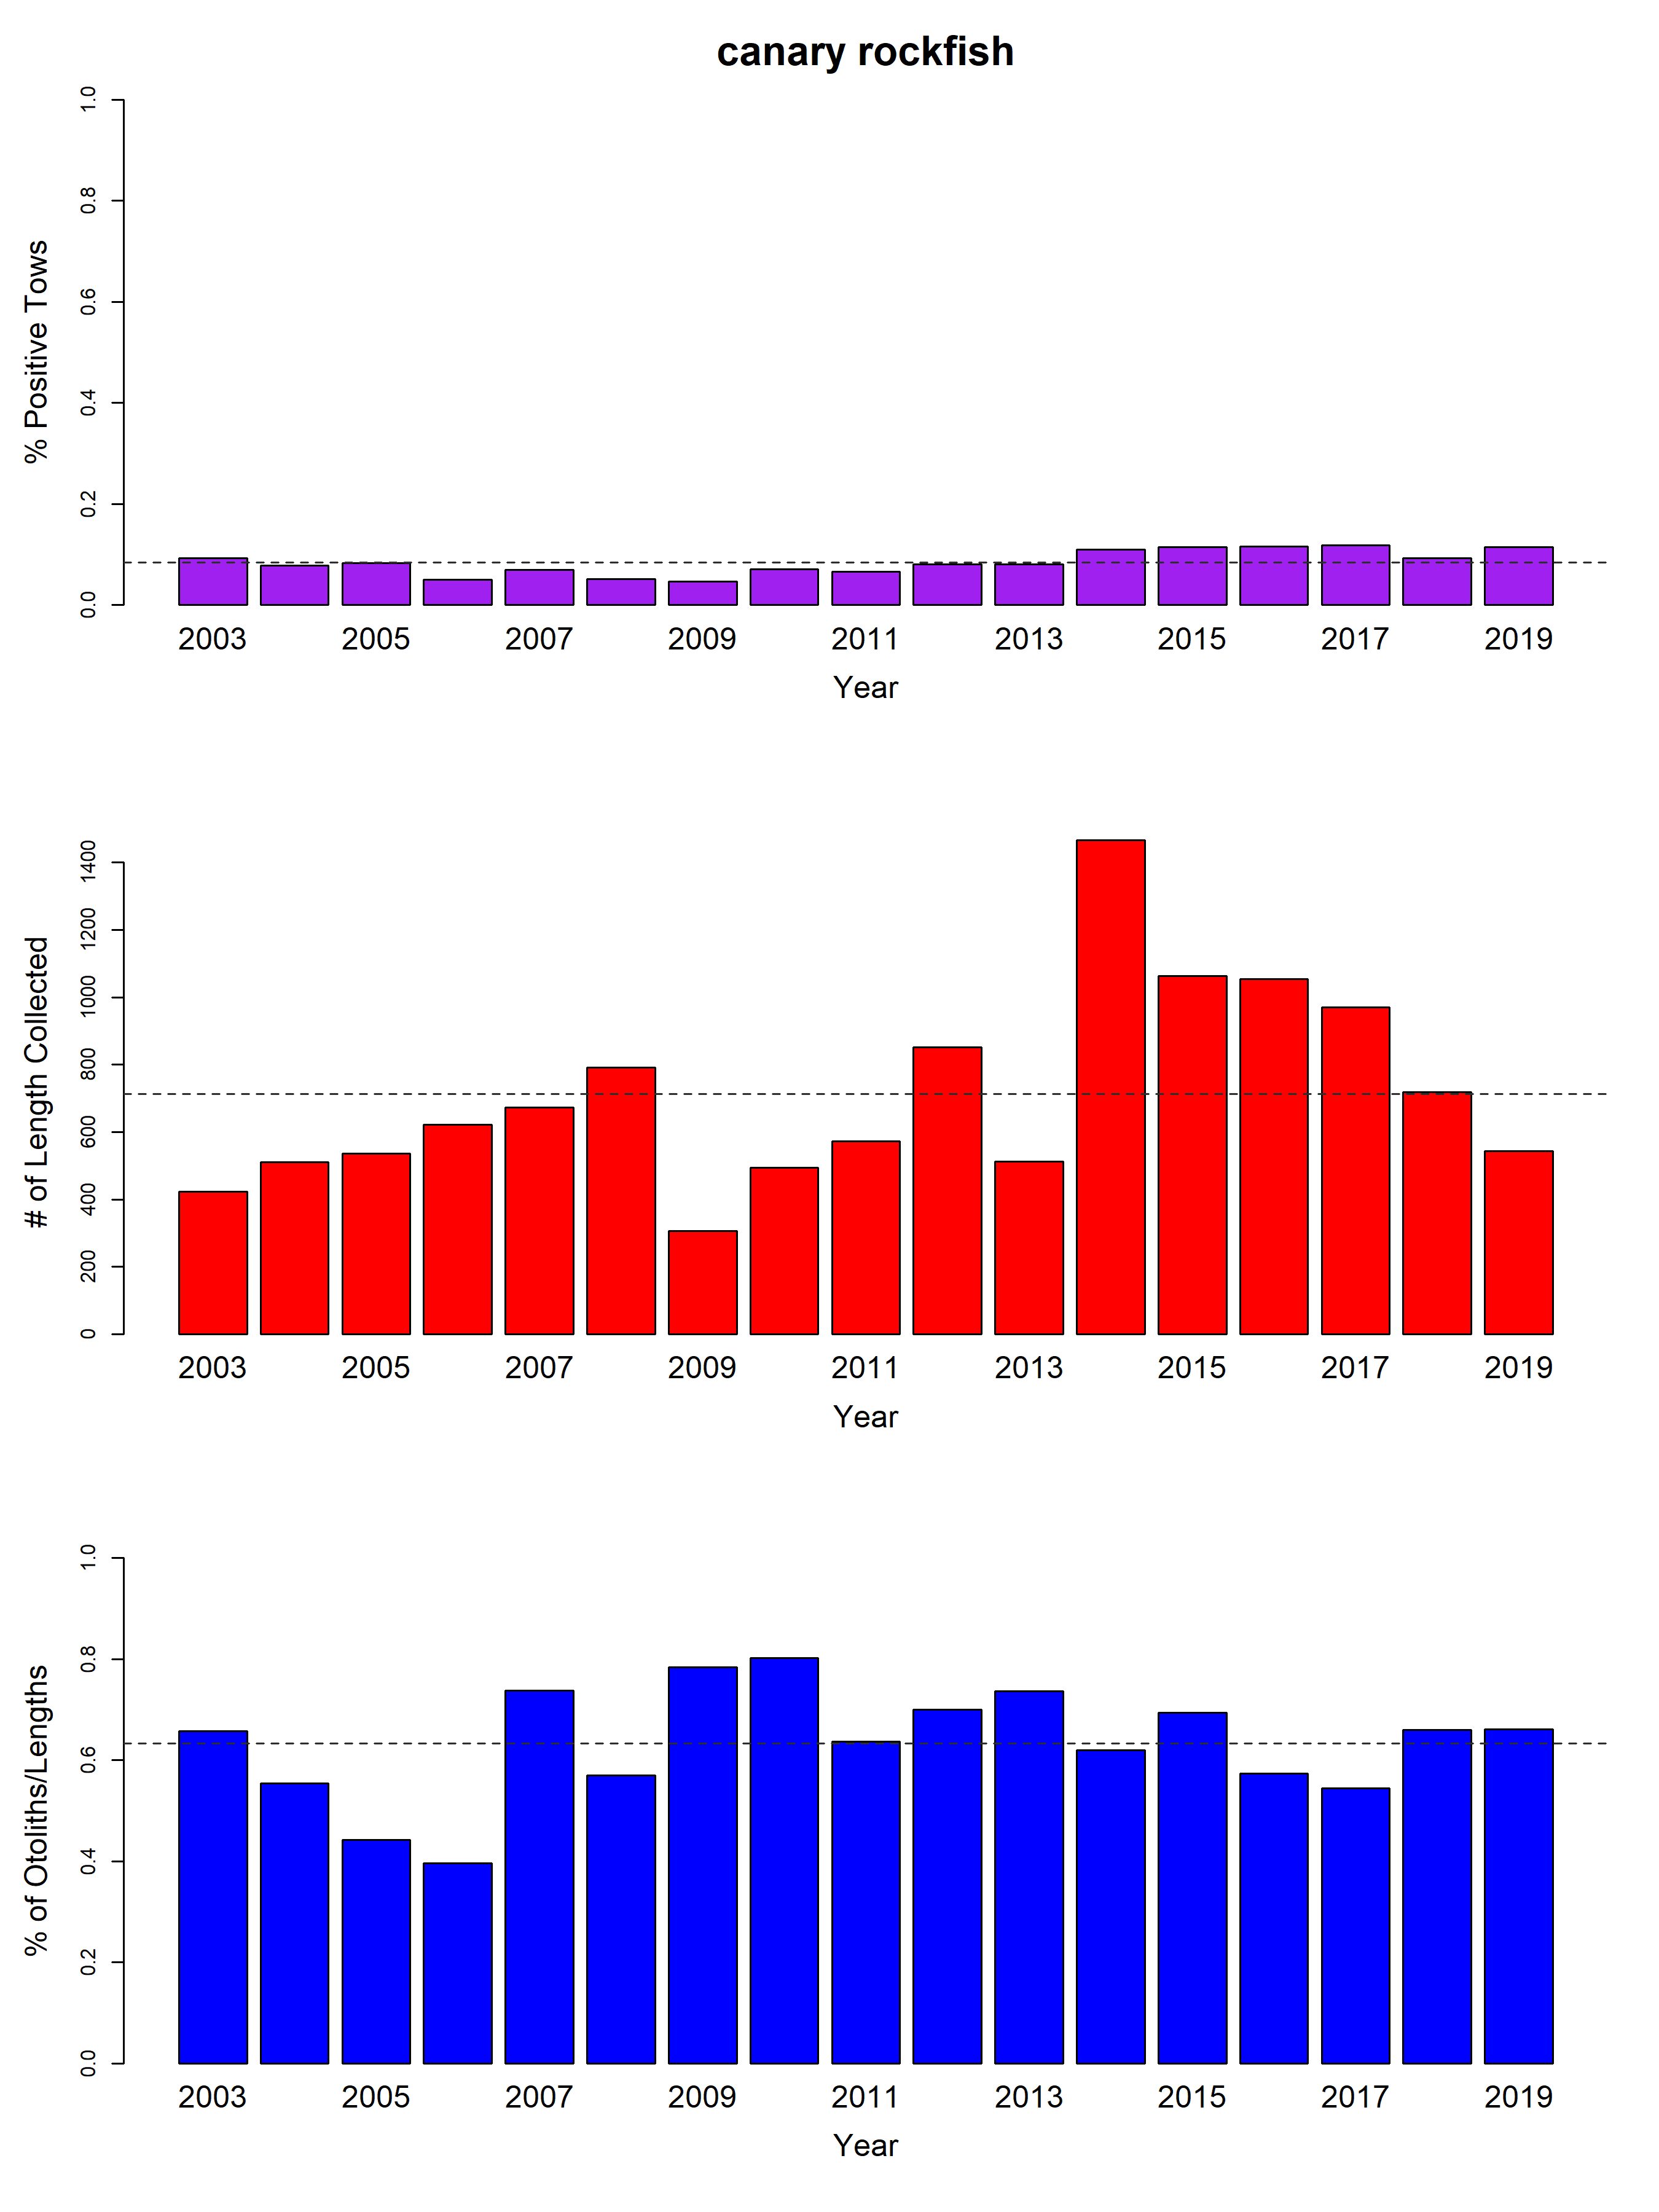
\includegraphics[width=0.6\textwidth,height=\textheight]{C:/Assessments/2020/survey_summary/sum_plots/canary_rockfish_survey_stats.png}
\FloatBarrier  

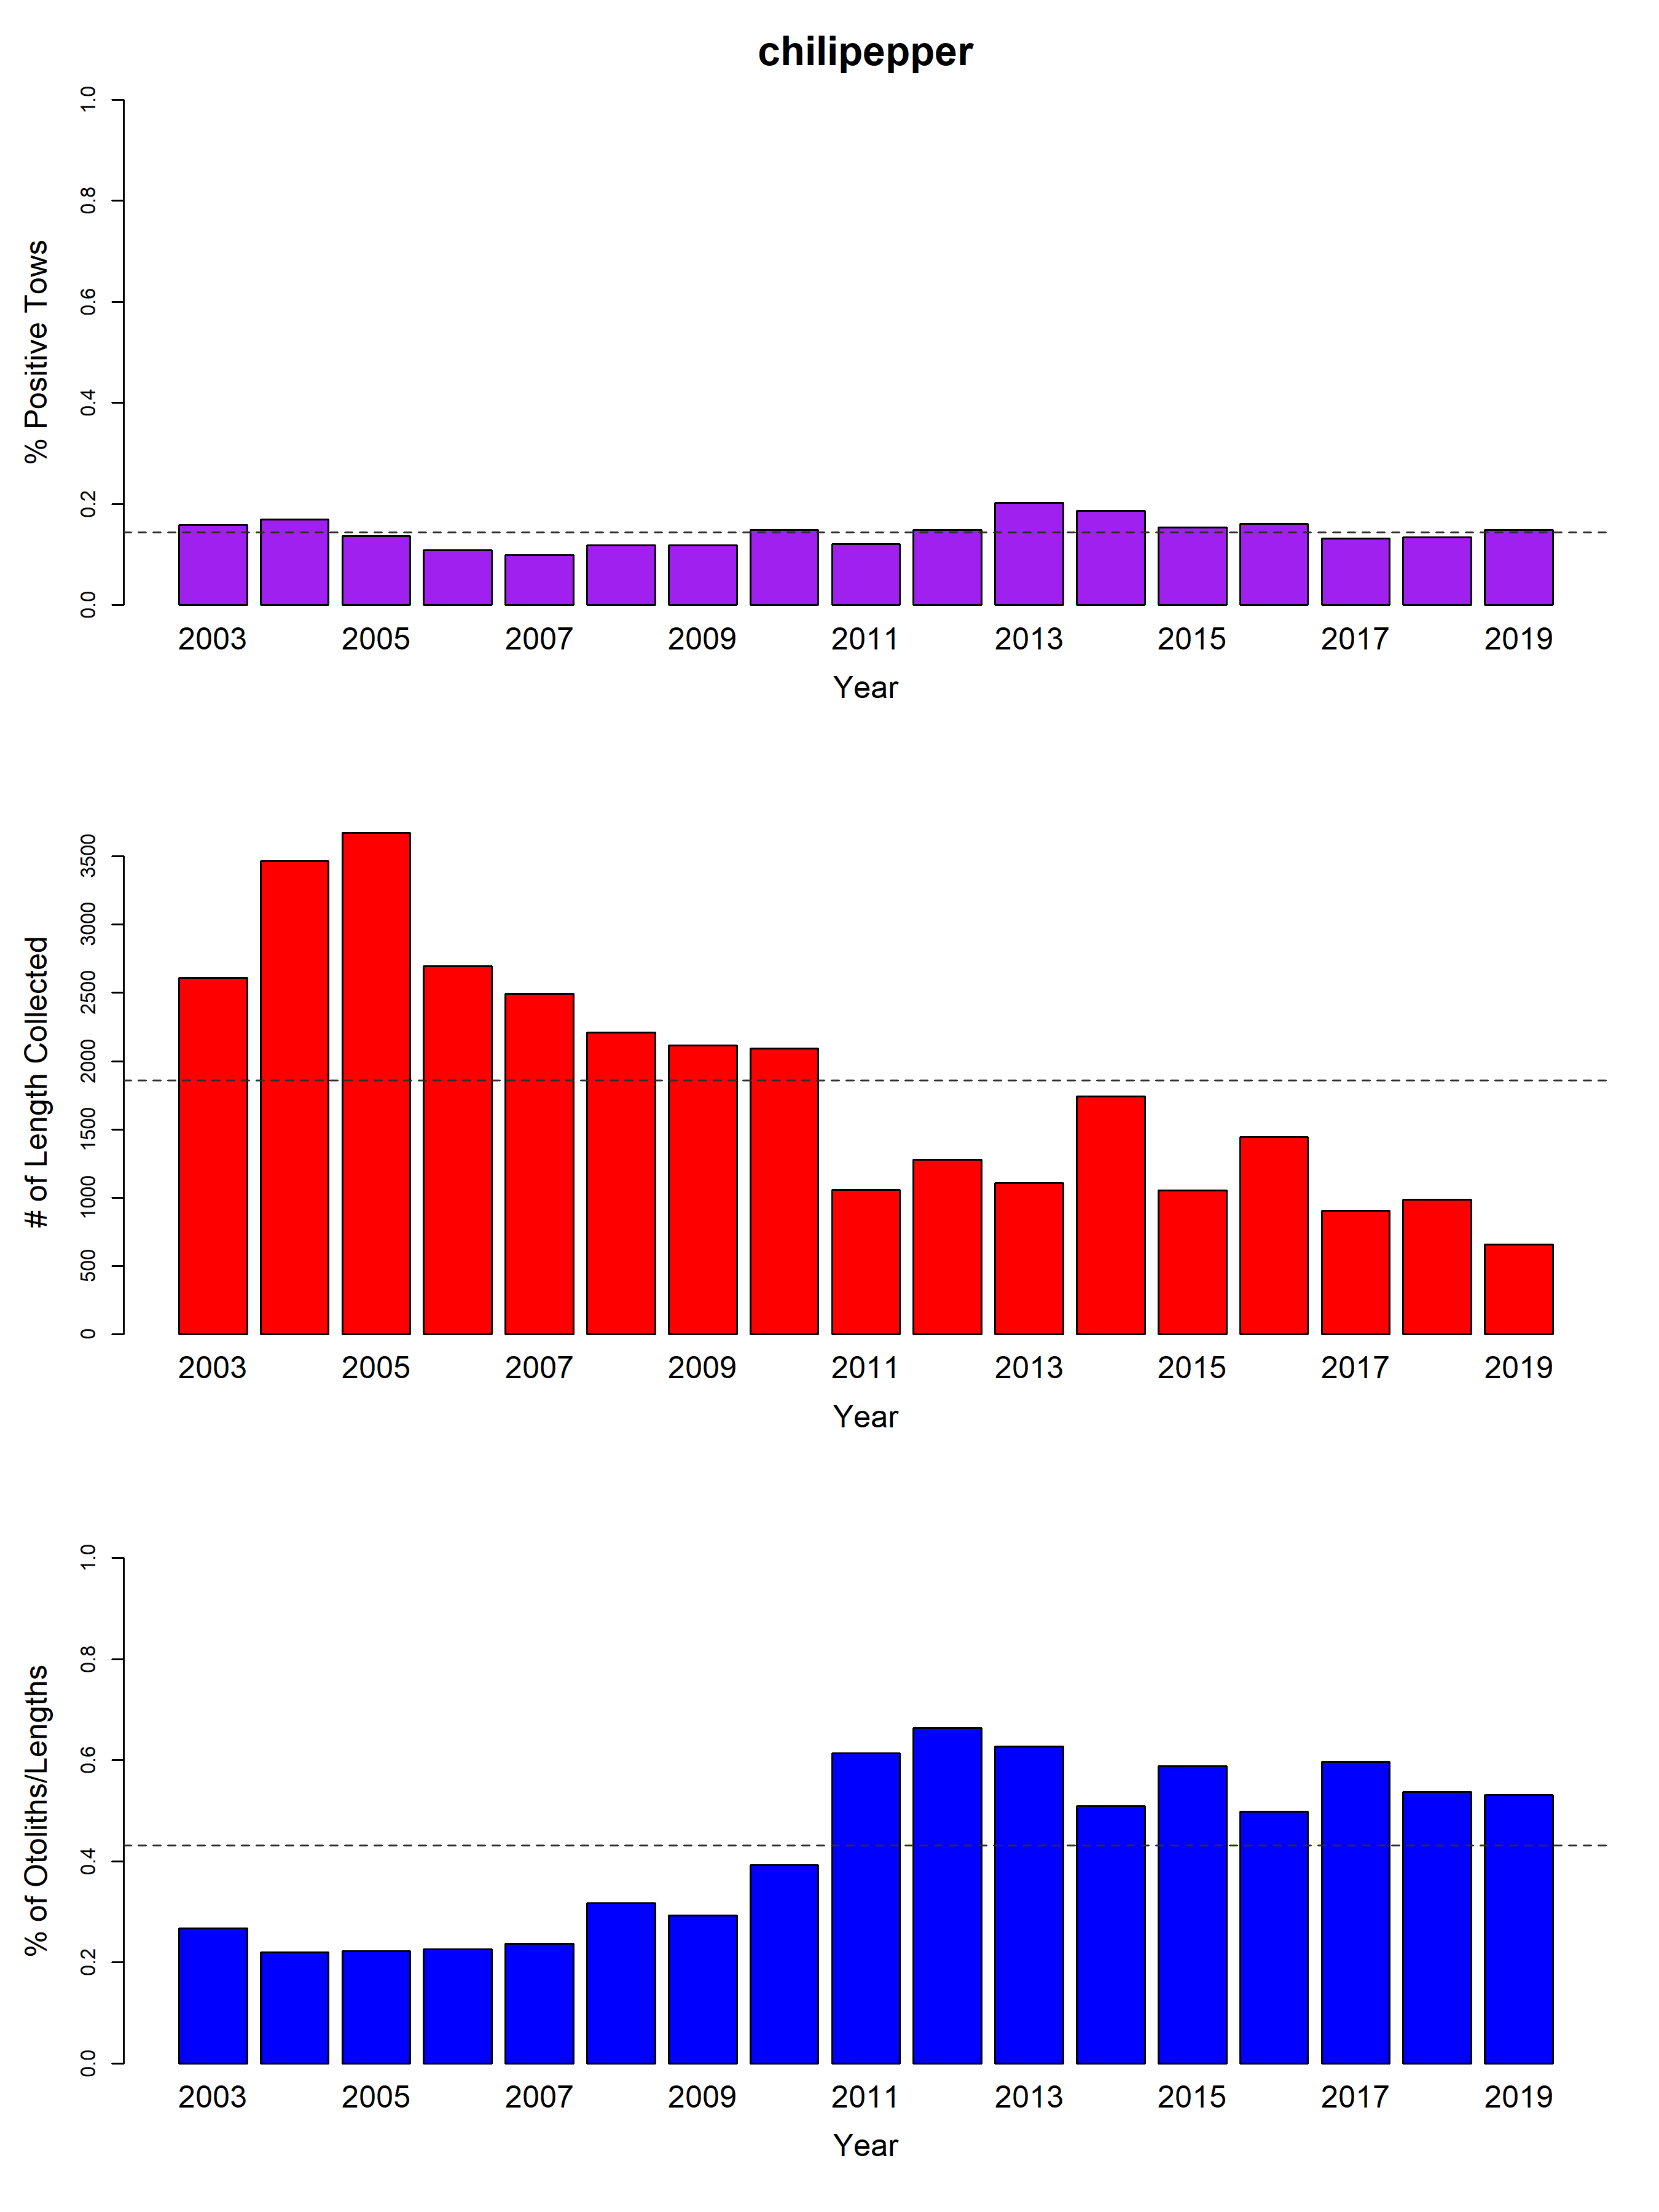
\includegraphics[width=0.6\textwidth,height=\textheight]{C:/Assessments/2020/survey_summary/sum_plots/chilipepper_survey_stats.png}
\FloatBarrier  

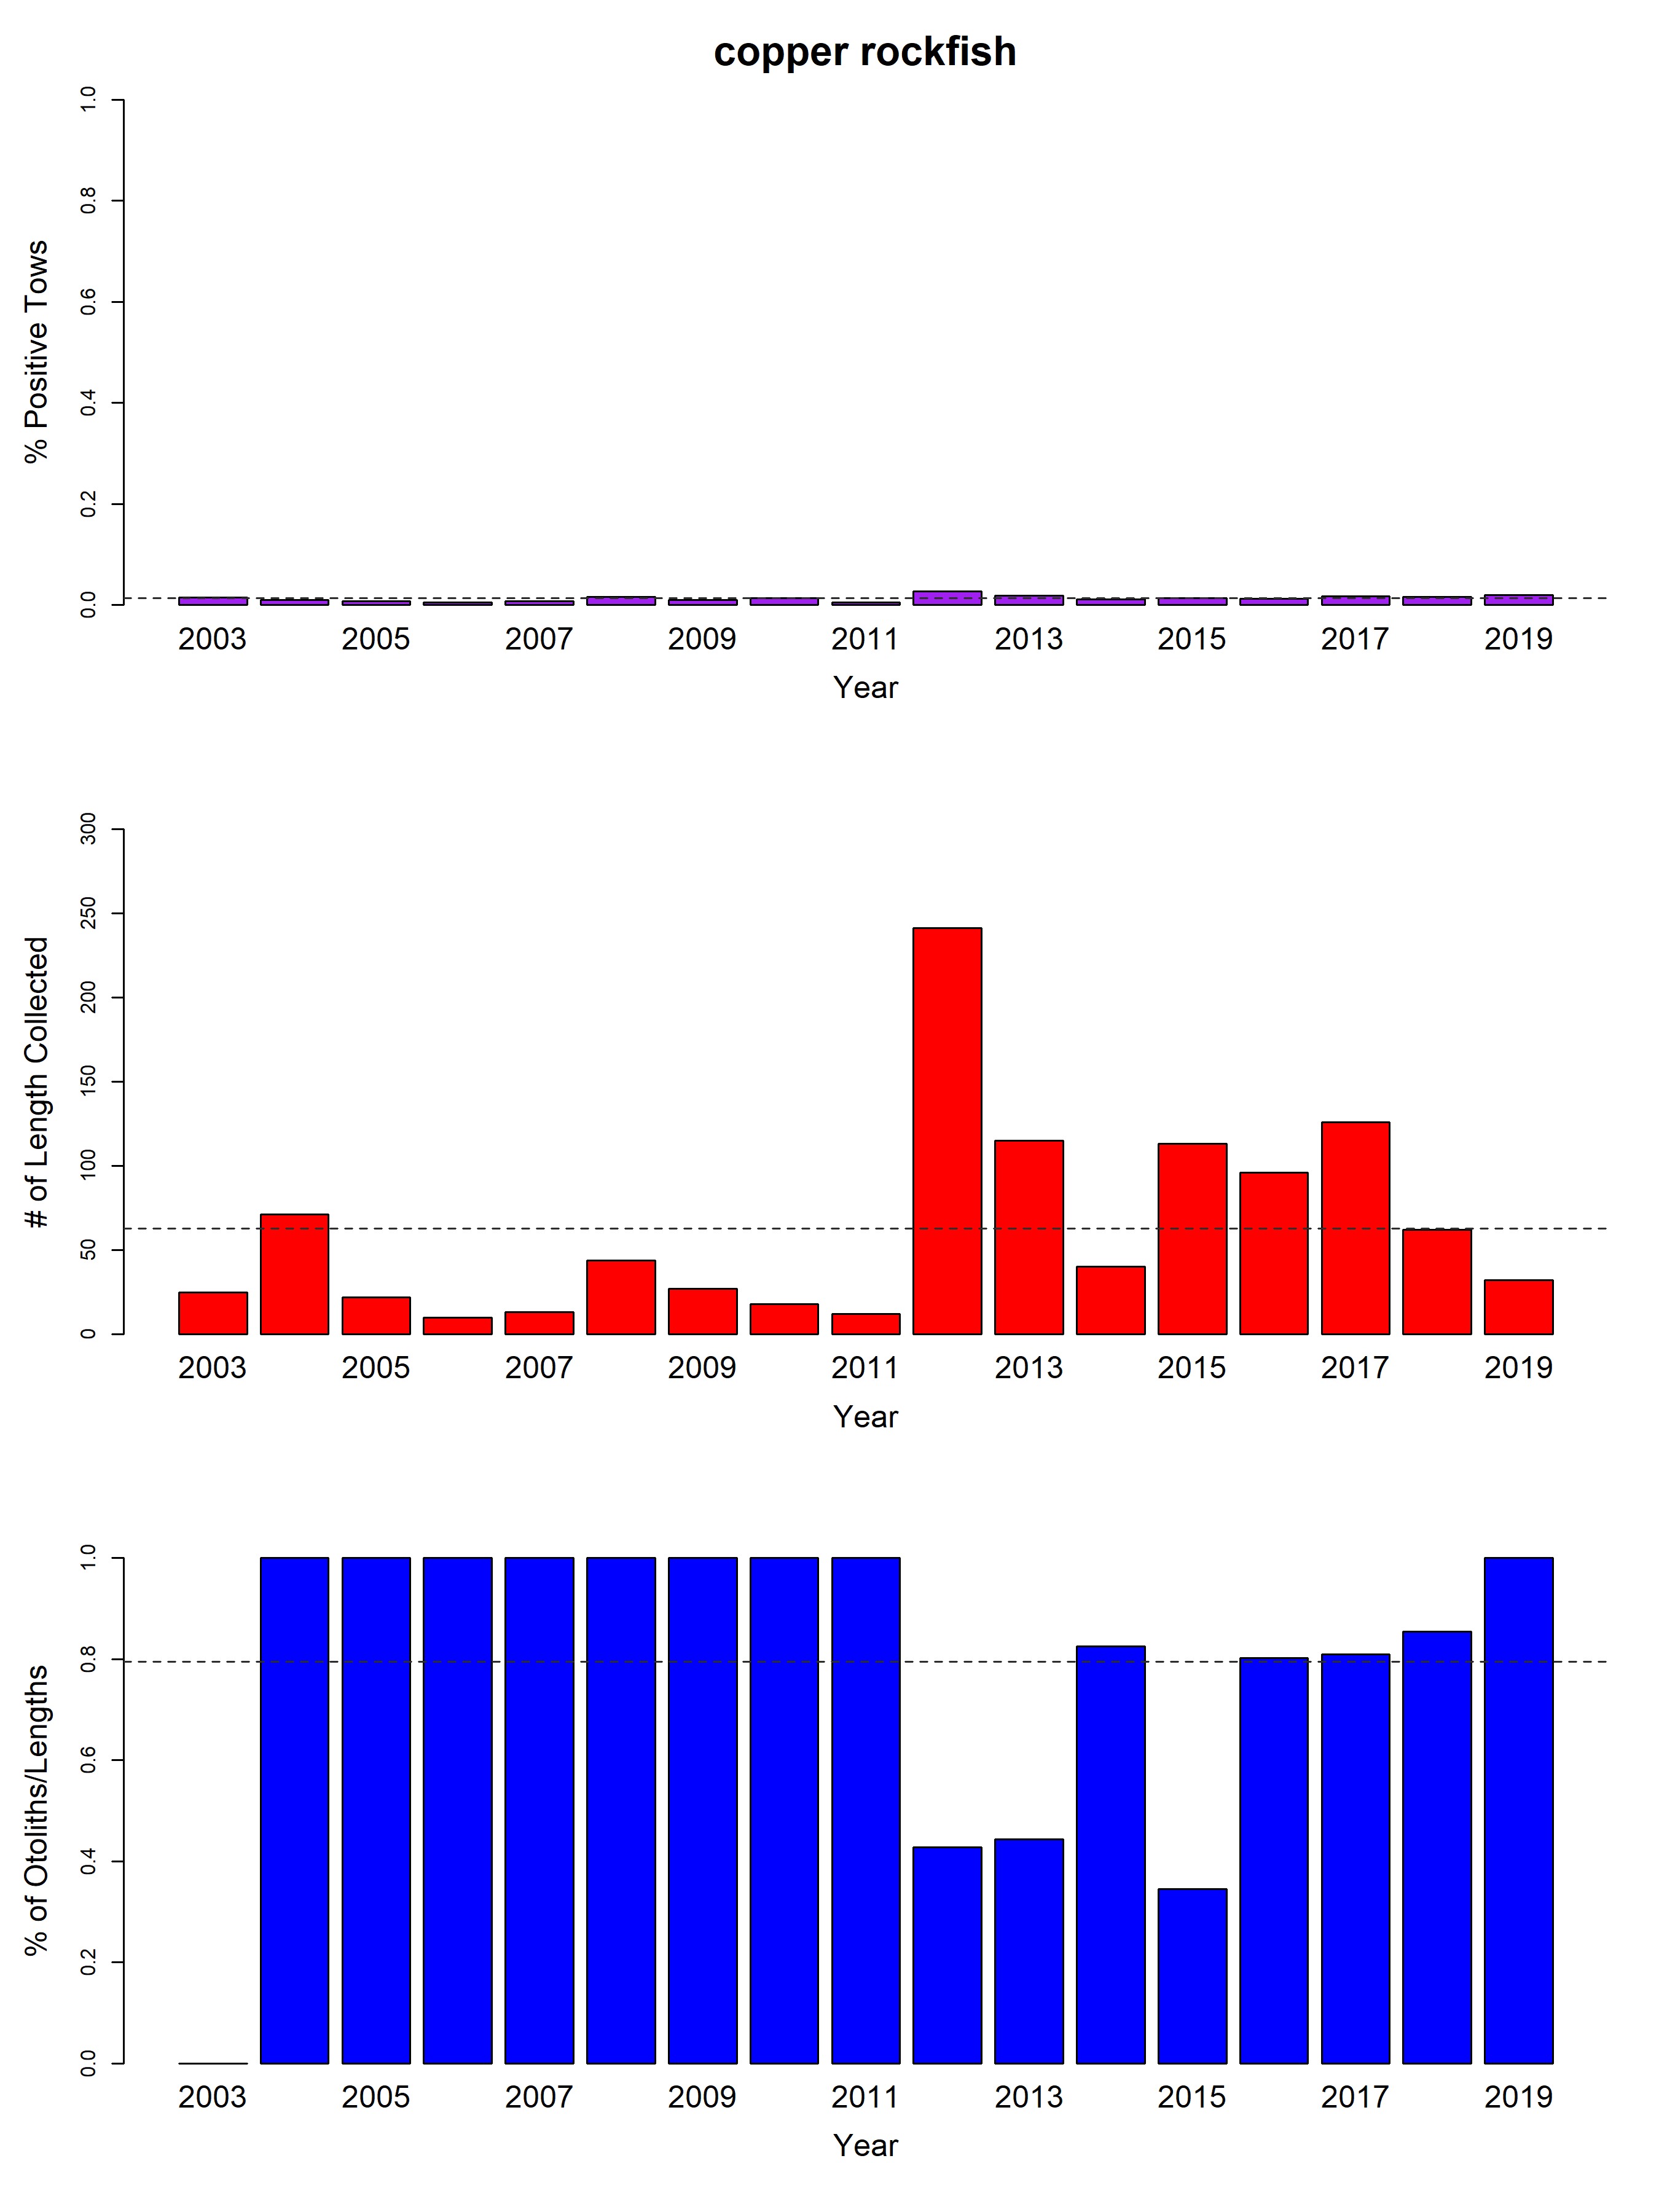
\includegraphics[width=0.6\textwidth,height=\textheight]{C:/Assessments/2020/survey_summary/sum_plots/copper_rockfish_survey_stats.png}
\FloatBarrier  

\FloatBarrier

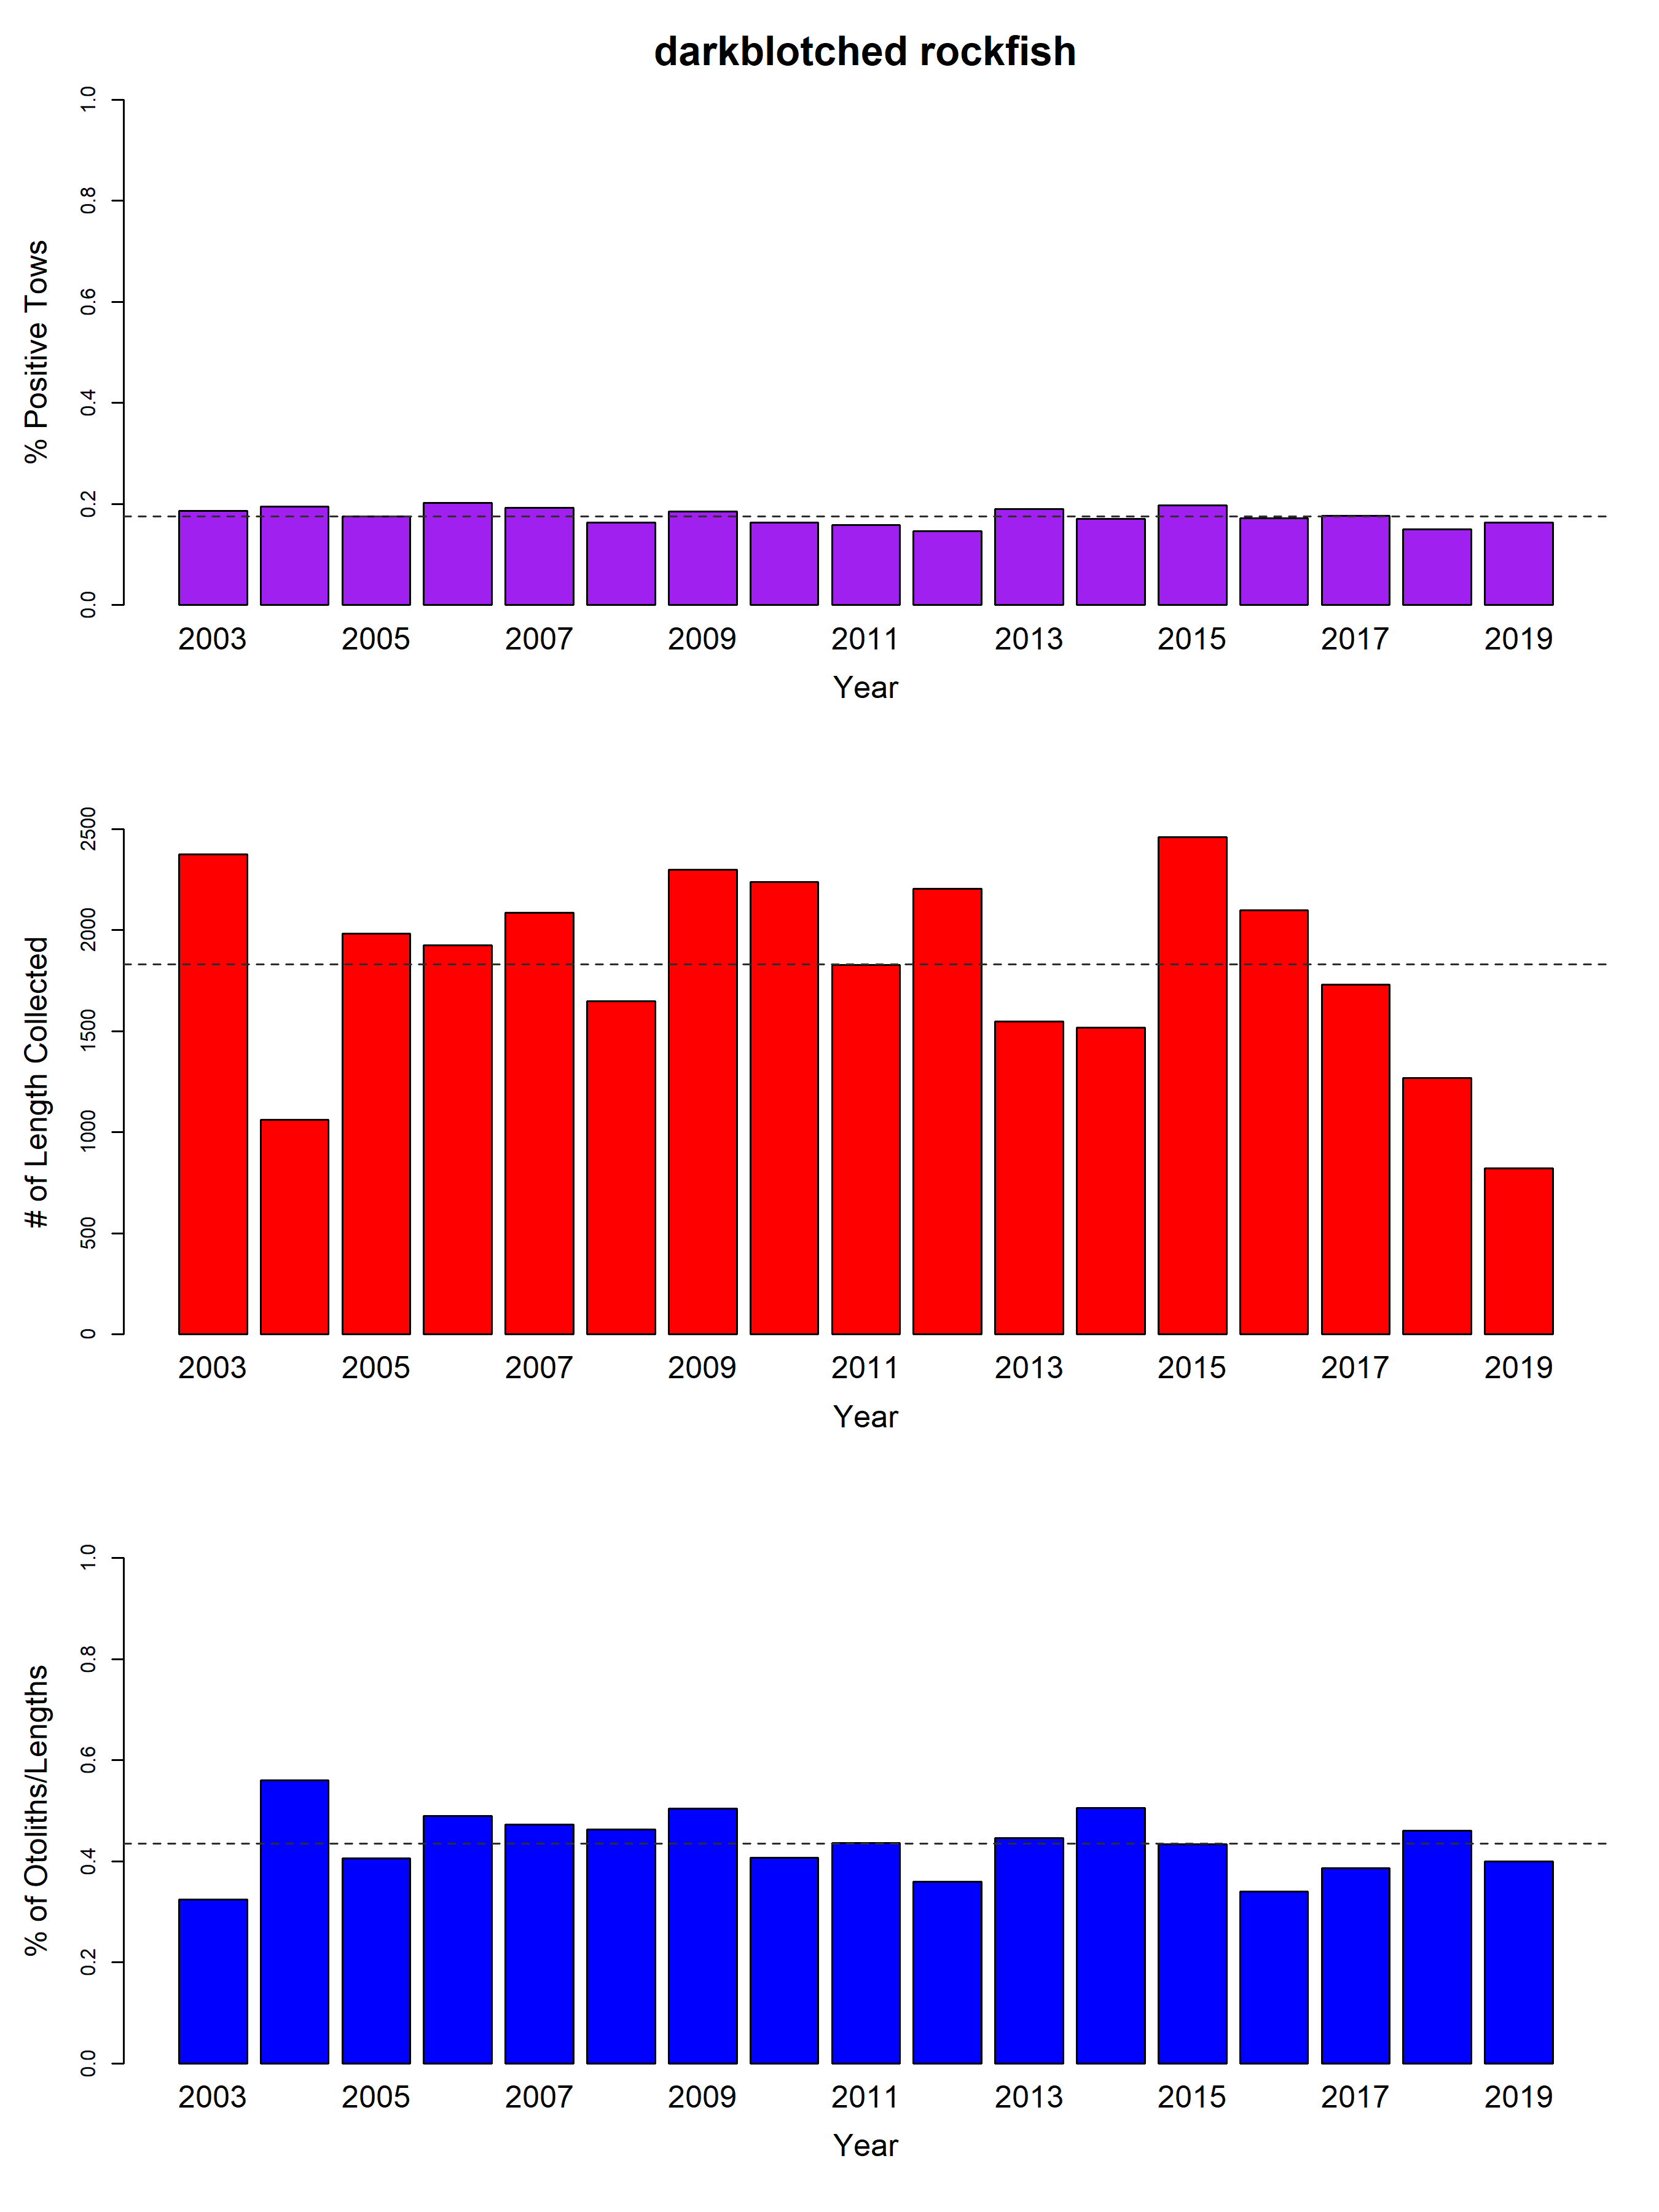
\includegraphics[width=0.6\textwidth,height=\textheight]{C:/Assessments/2020/survey_summary/sum_plots/darkblotched_rockfish_survey_stats.png}
\FloatBarrier  

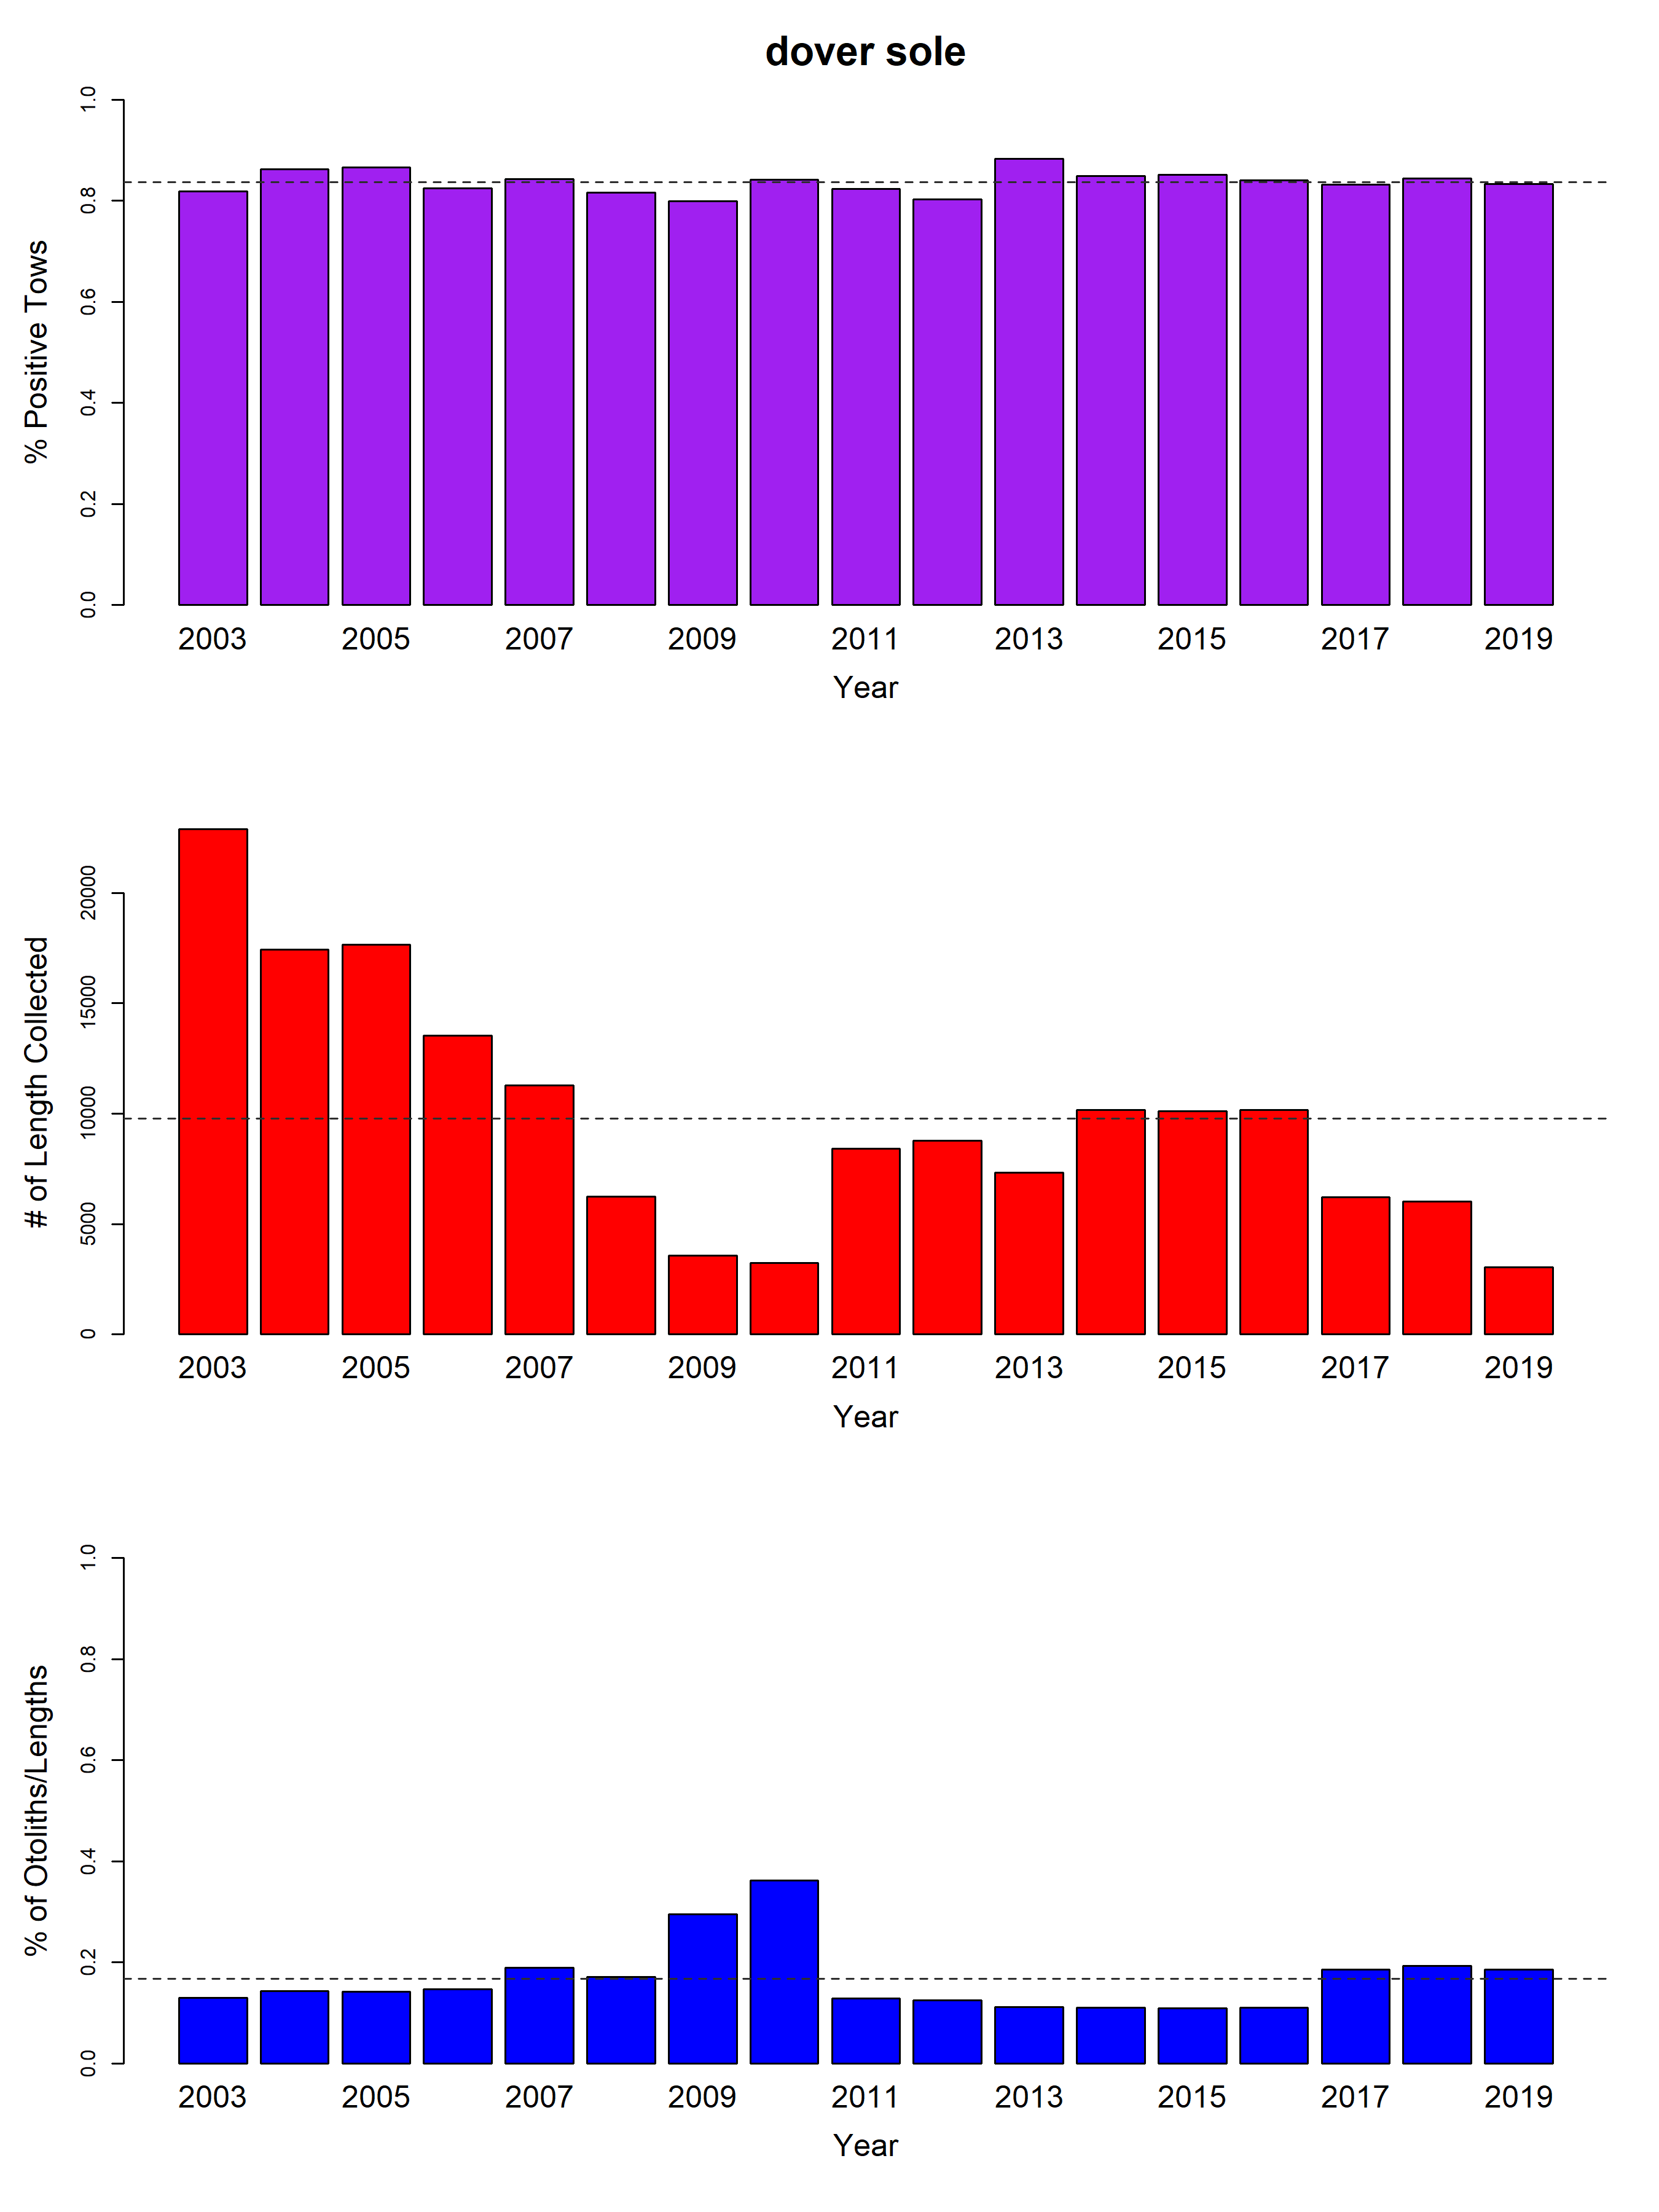
\includegraphics[width=0.6\textwidth,height=\textheight]{C:/Assessments/2020/survey_summary/sum_plots/dover_sole_survey_stats.png}
\FloatBarrier  

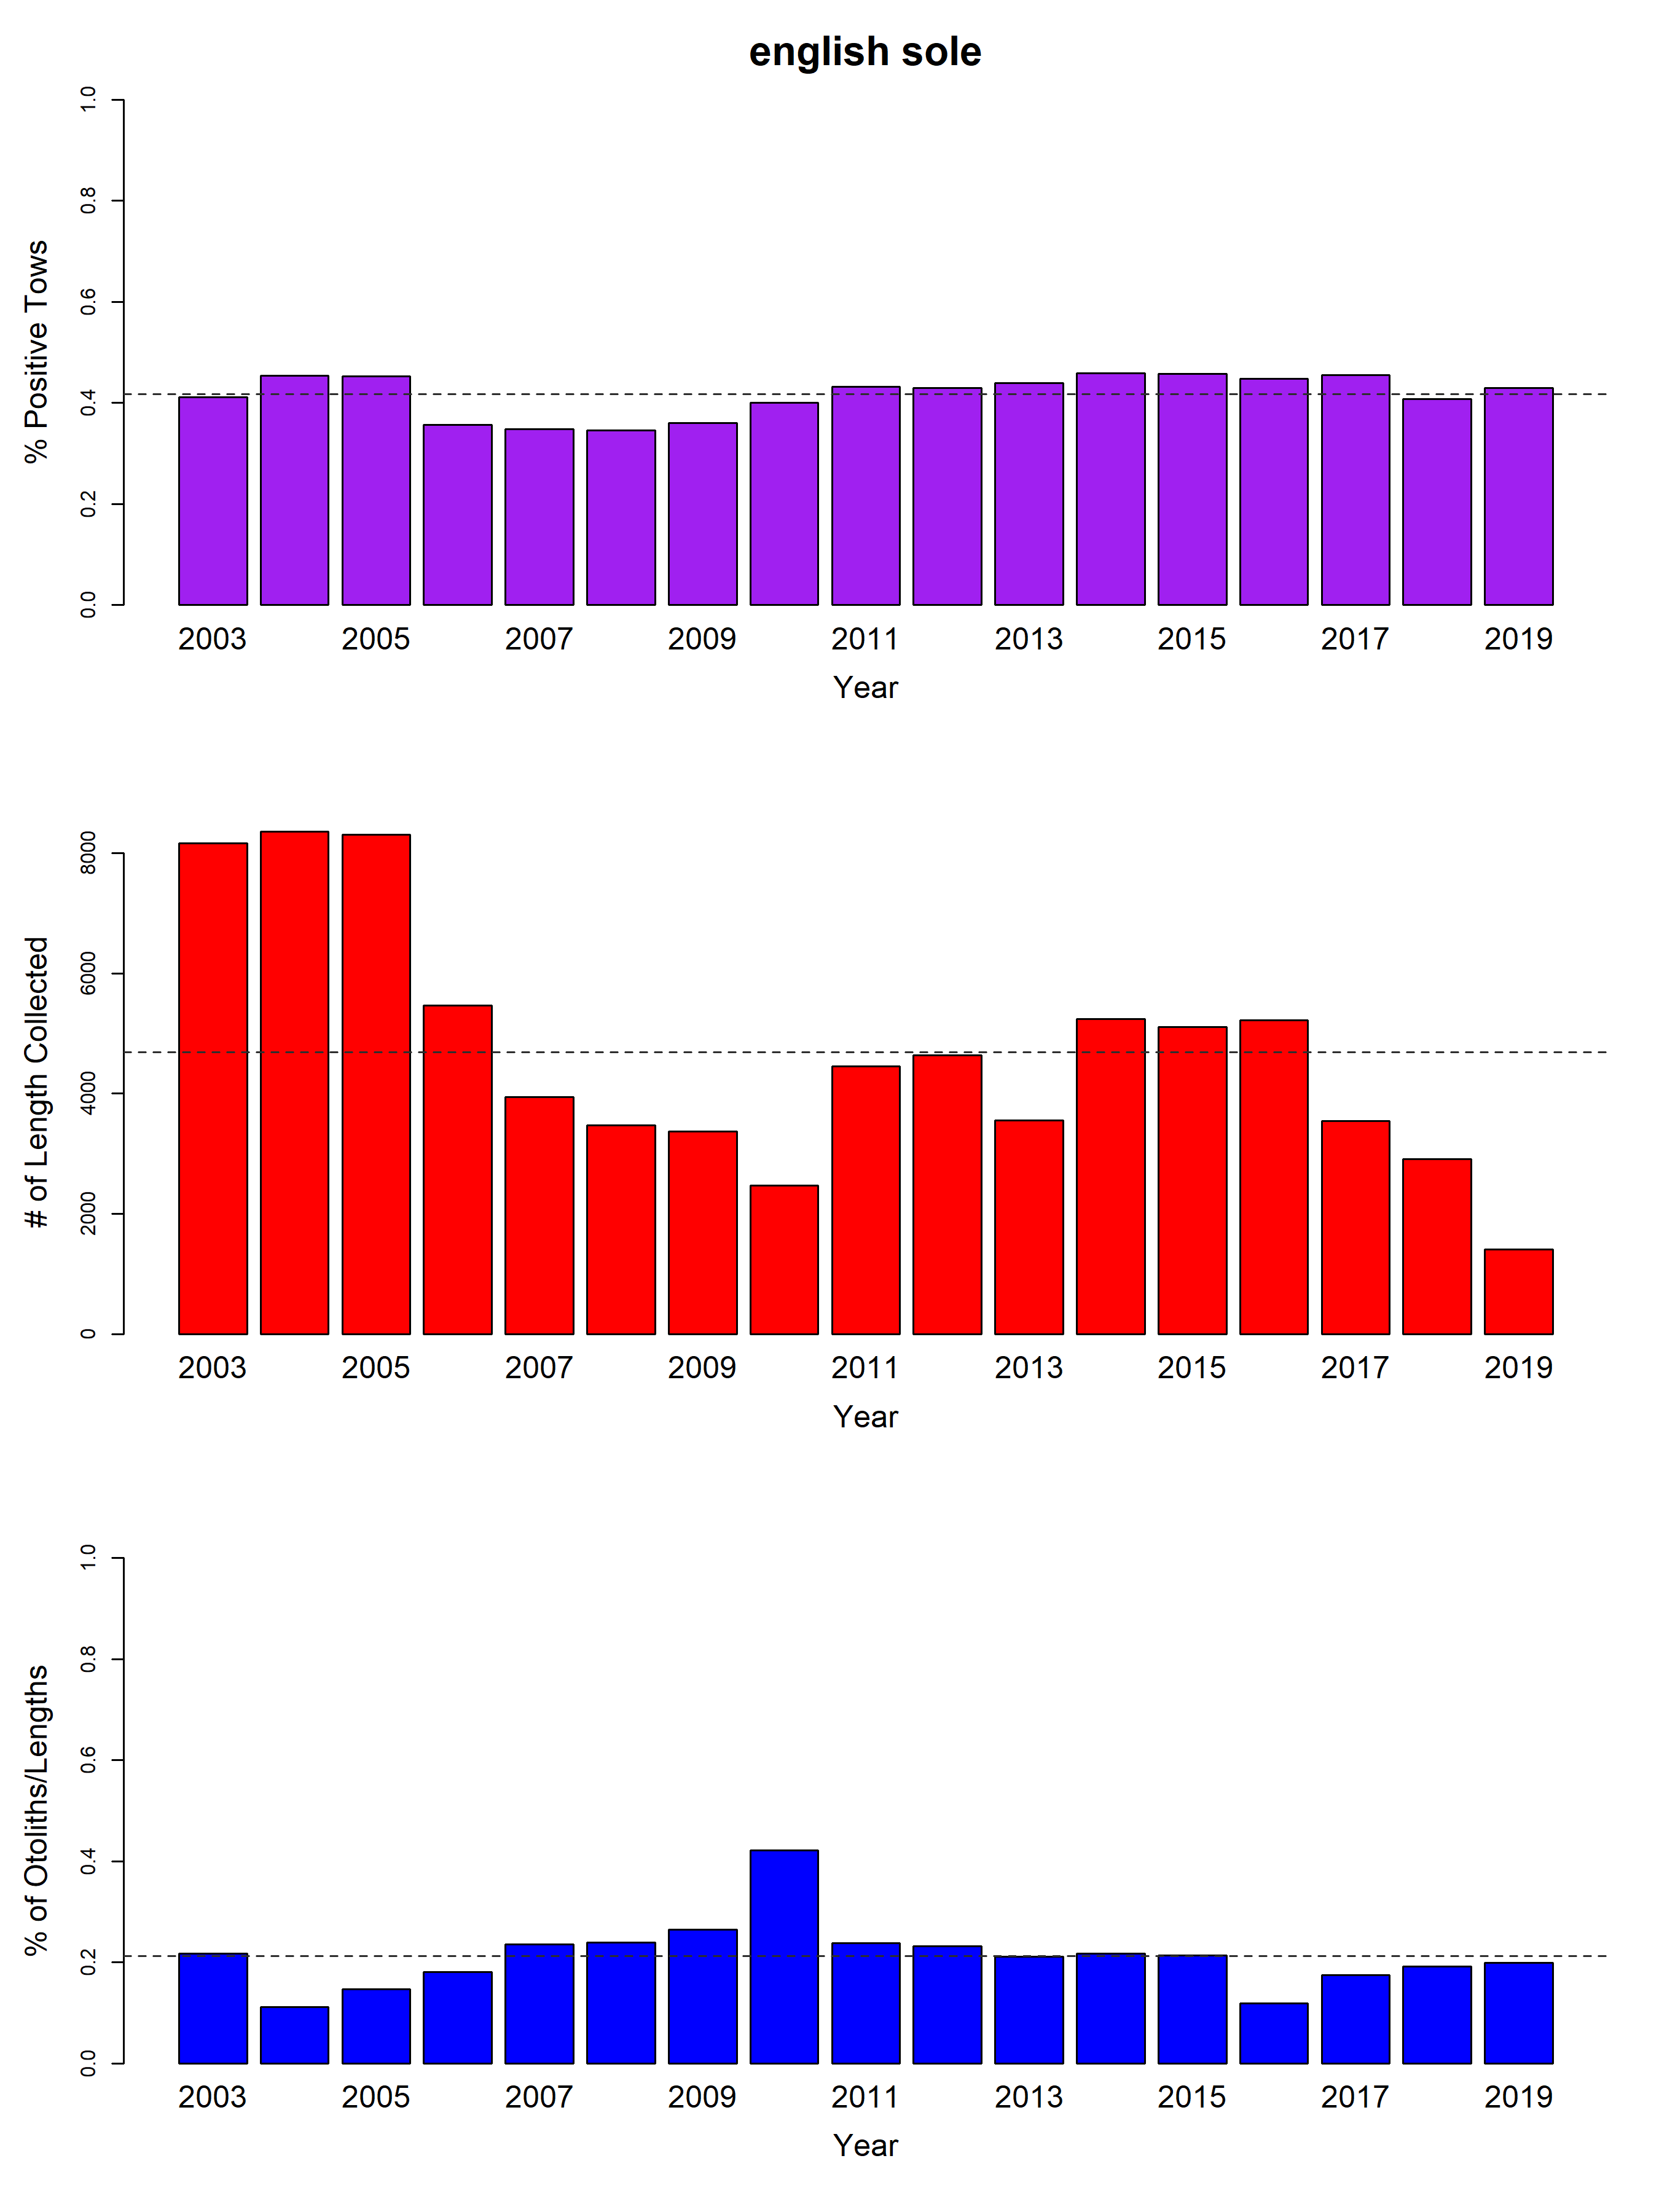
\includegraphics[width=0.6\textwidth,height=\textheight]{C:/Assessments/2020/survey_summary/sum_plots/english_sole_survey_stats.png}
\FloatBarrier  

\FloatBarrier

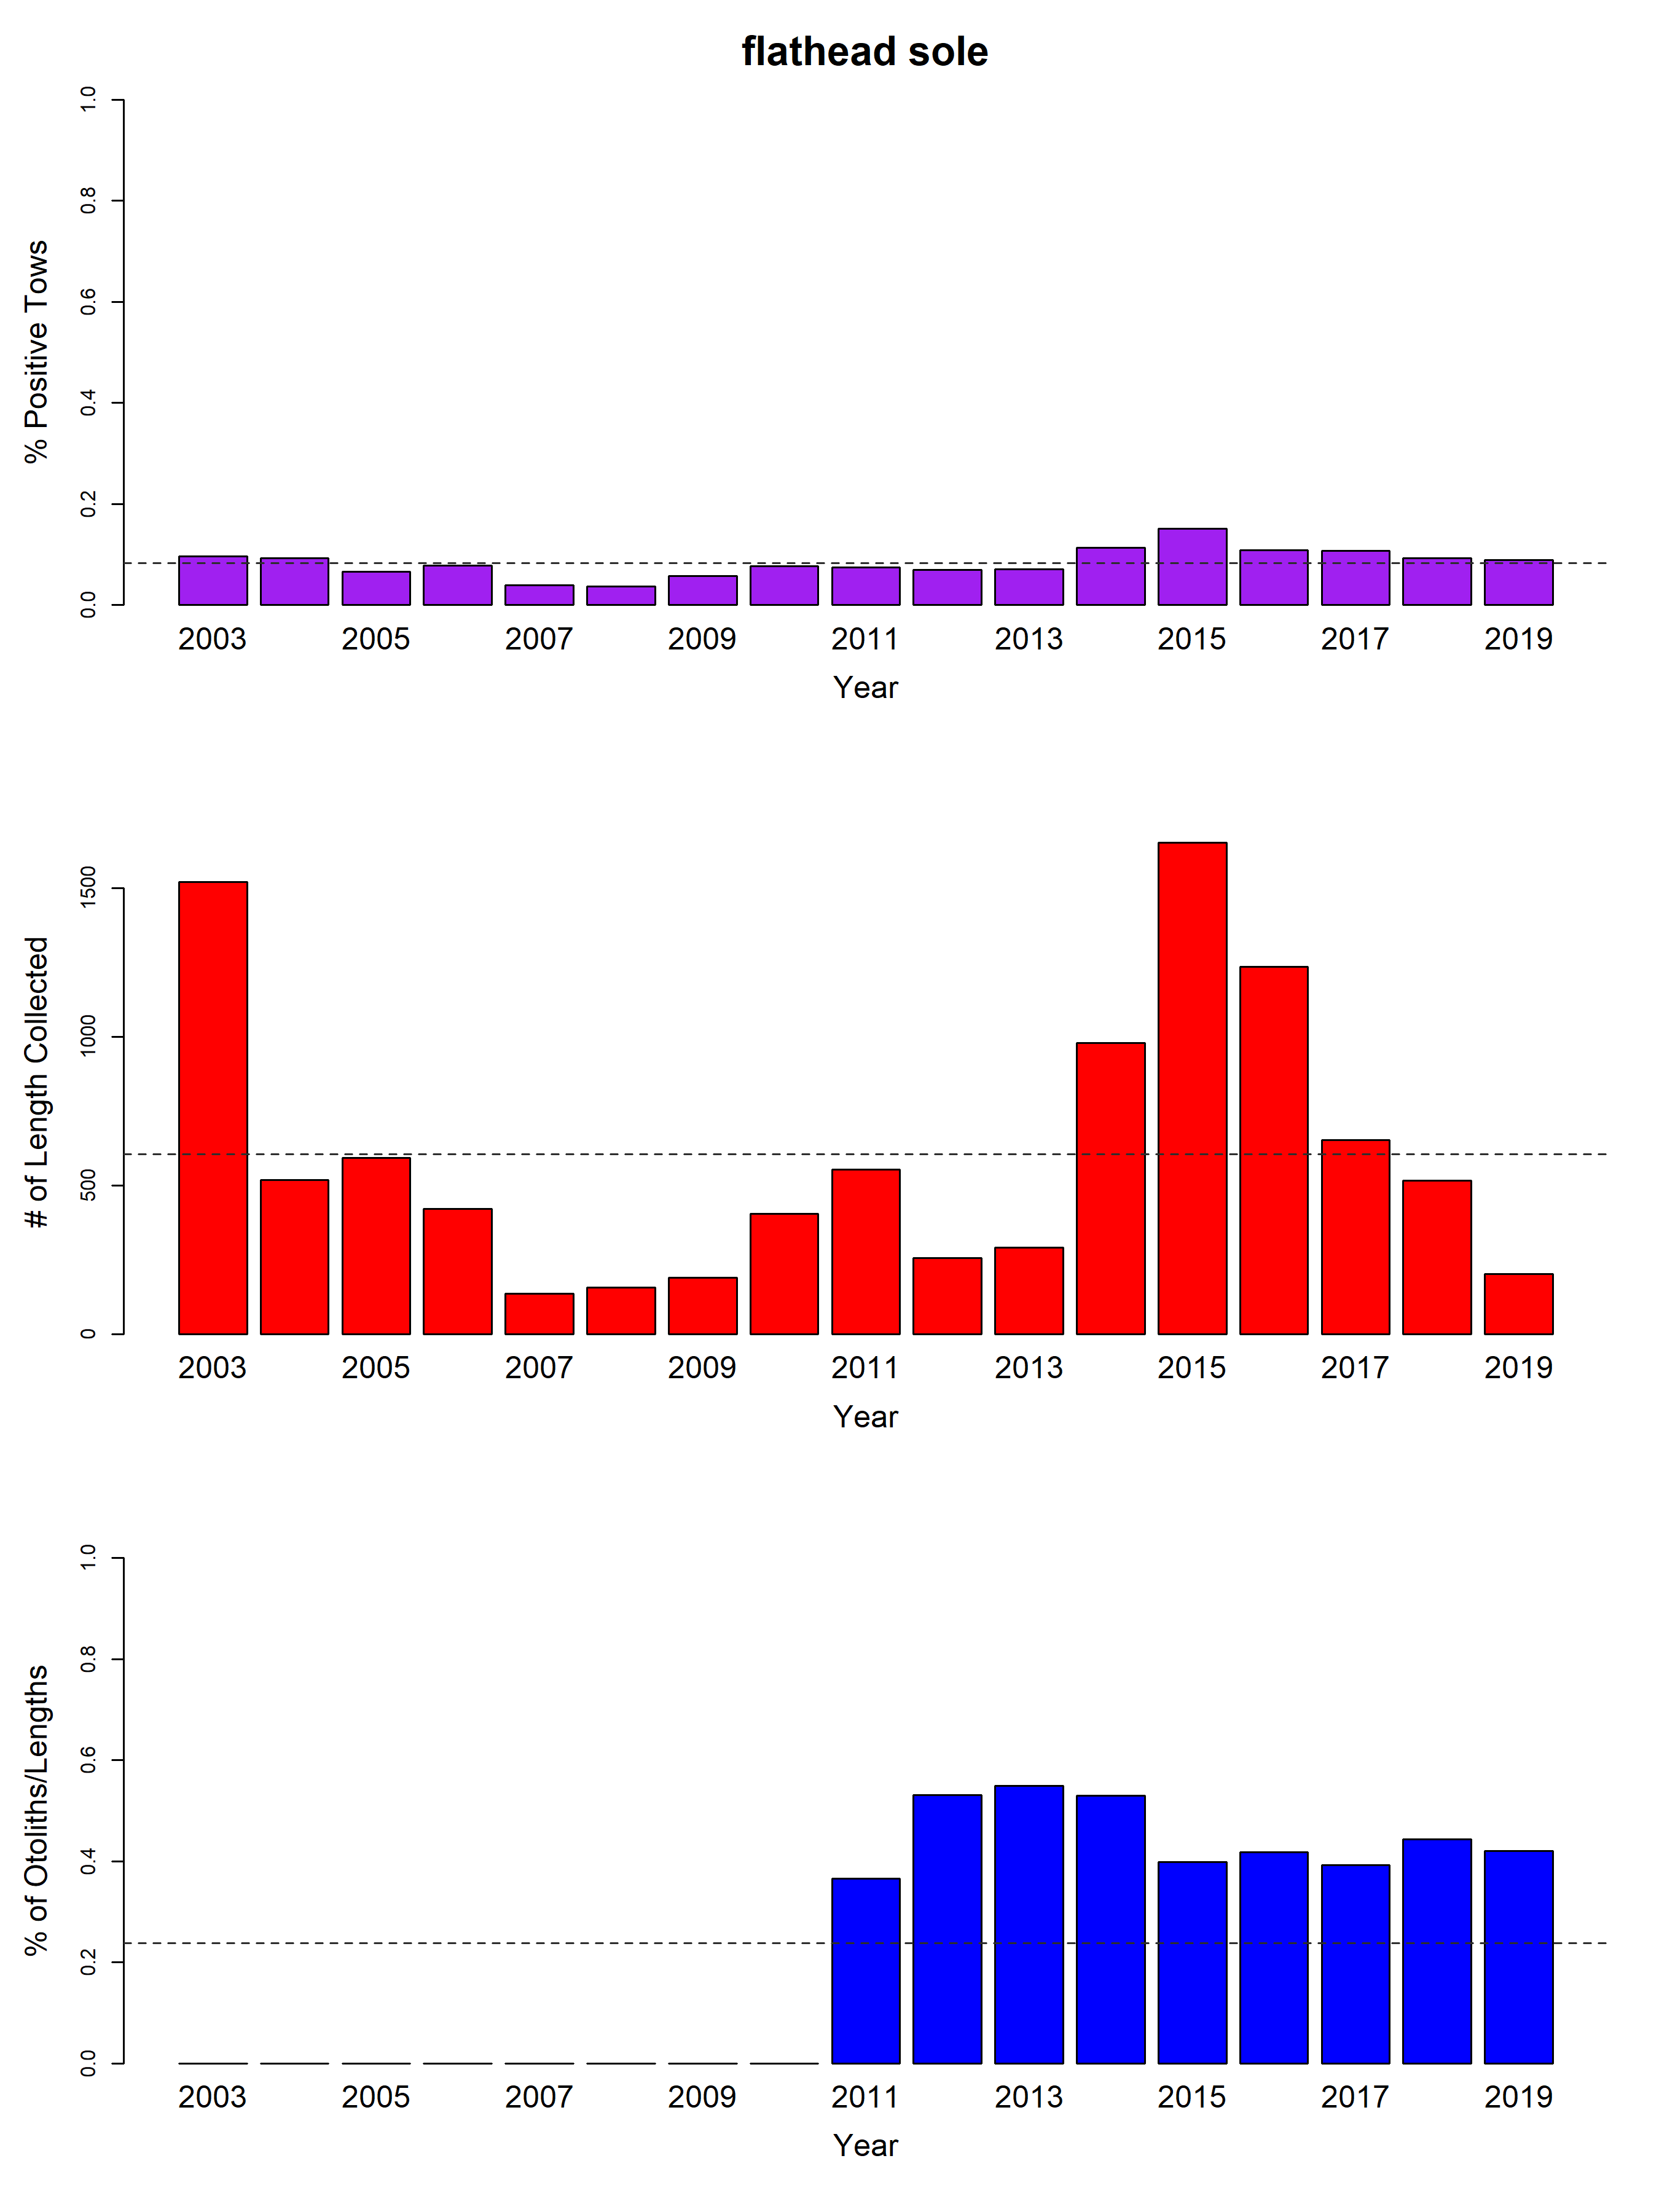
\includegraphics[width=0.6\textwidth,height=\textheight]{C:/Assessments/2020/survey_summary/sum_plots/flathead_sole_survey_stats.png}
\FloatBarrier  

\FloatBarrier

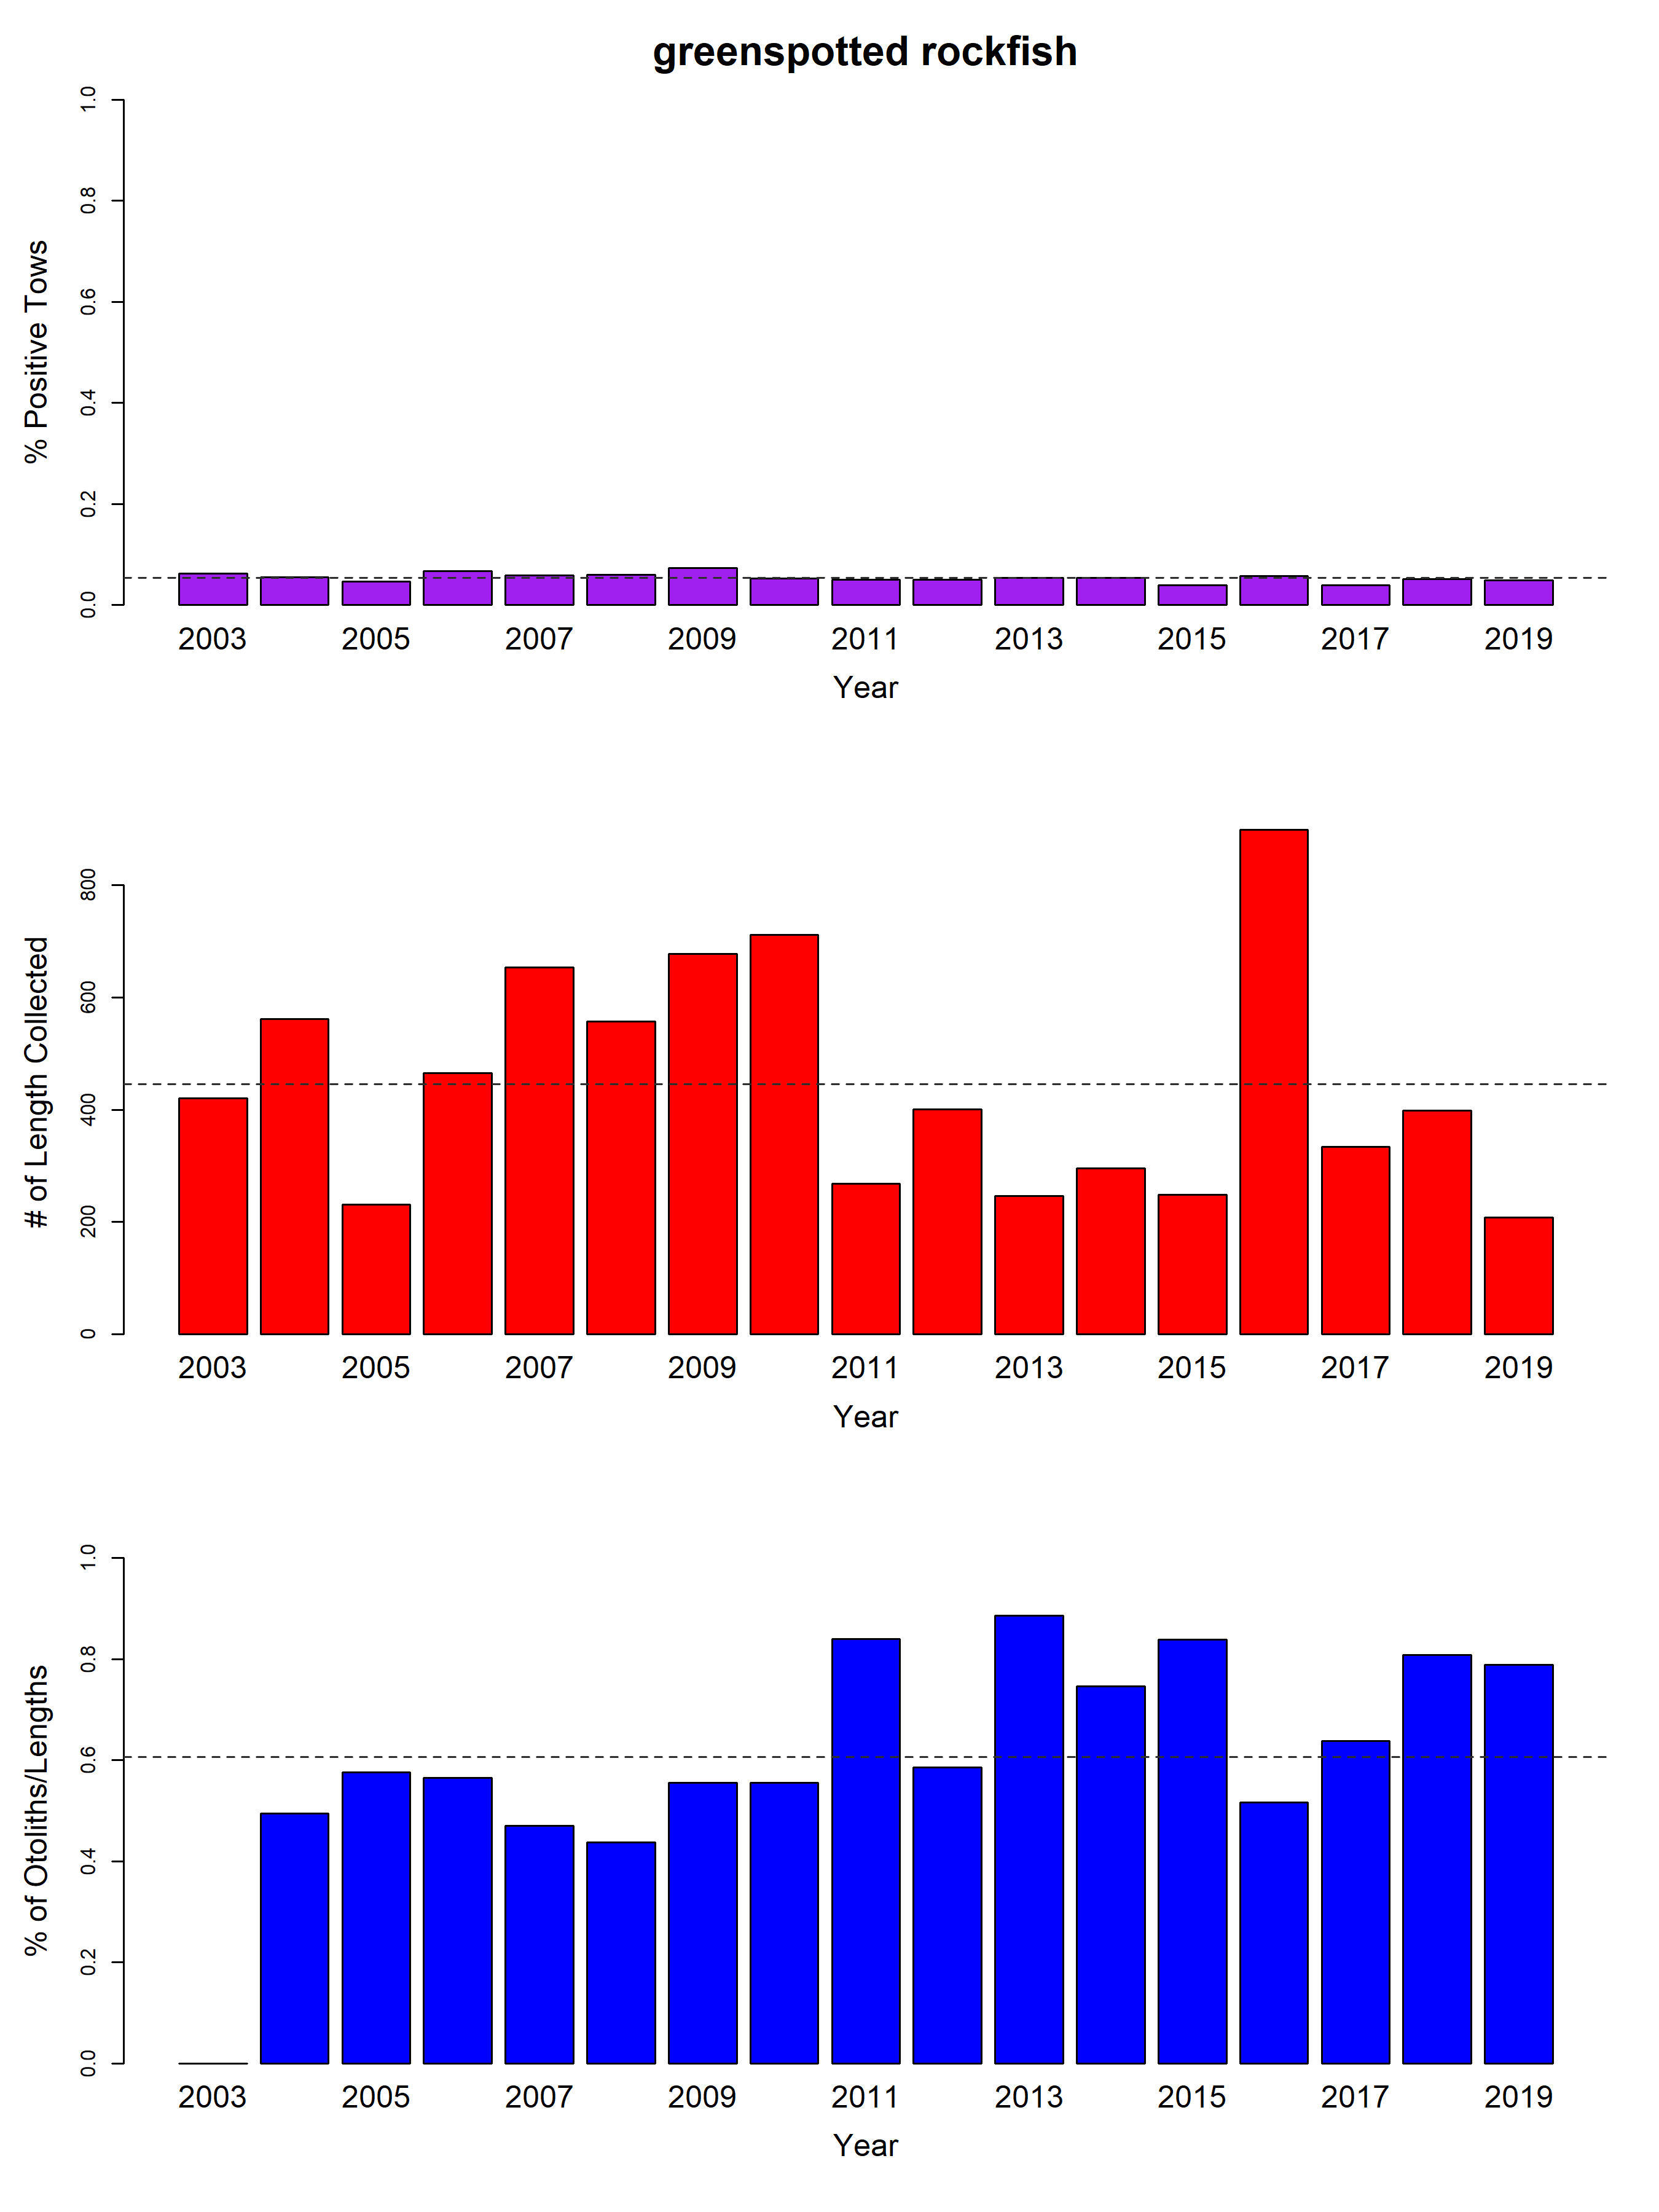
\includegraphics[width=0.6\textwidth,height=\textheight]{C:/Assessments/2020/survey_summary/sum_plots/greenspotted_rockfish_survey_stats.png}
\FloatBarrier  

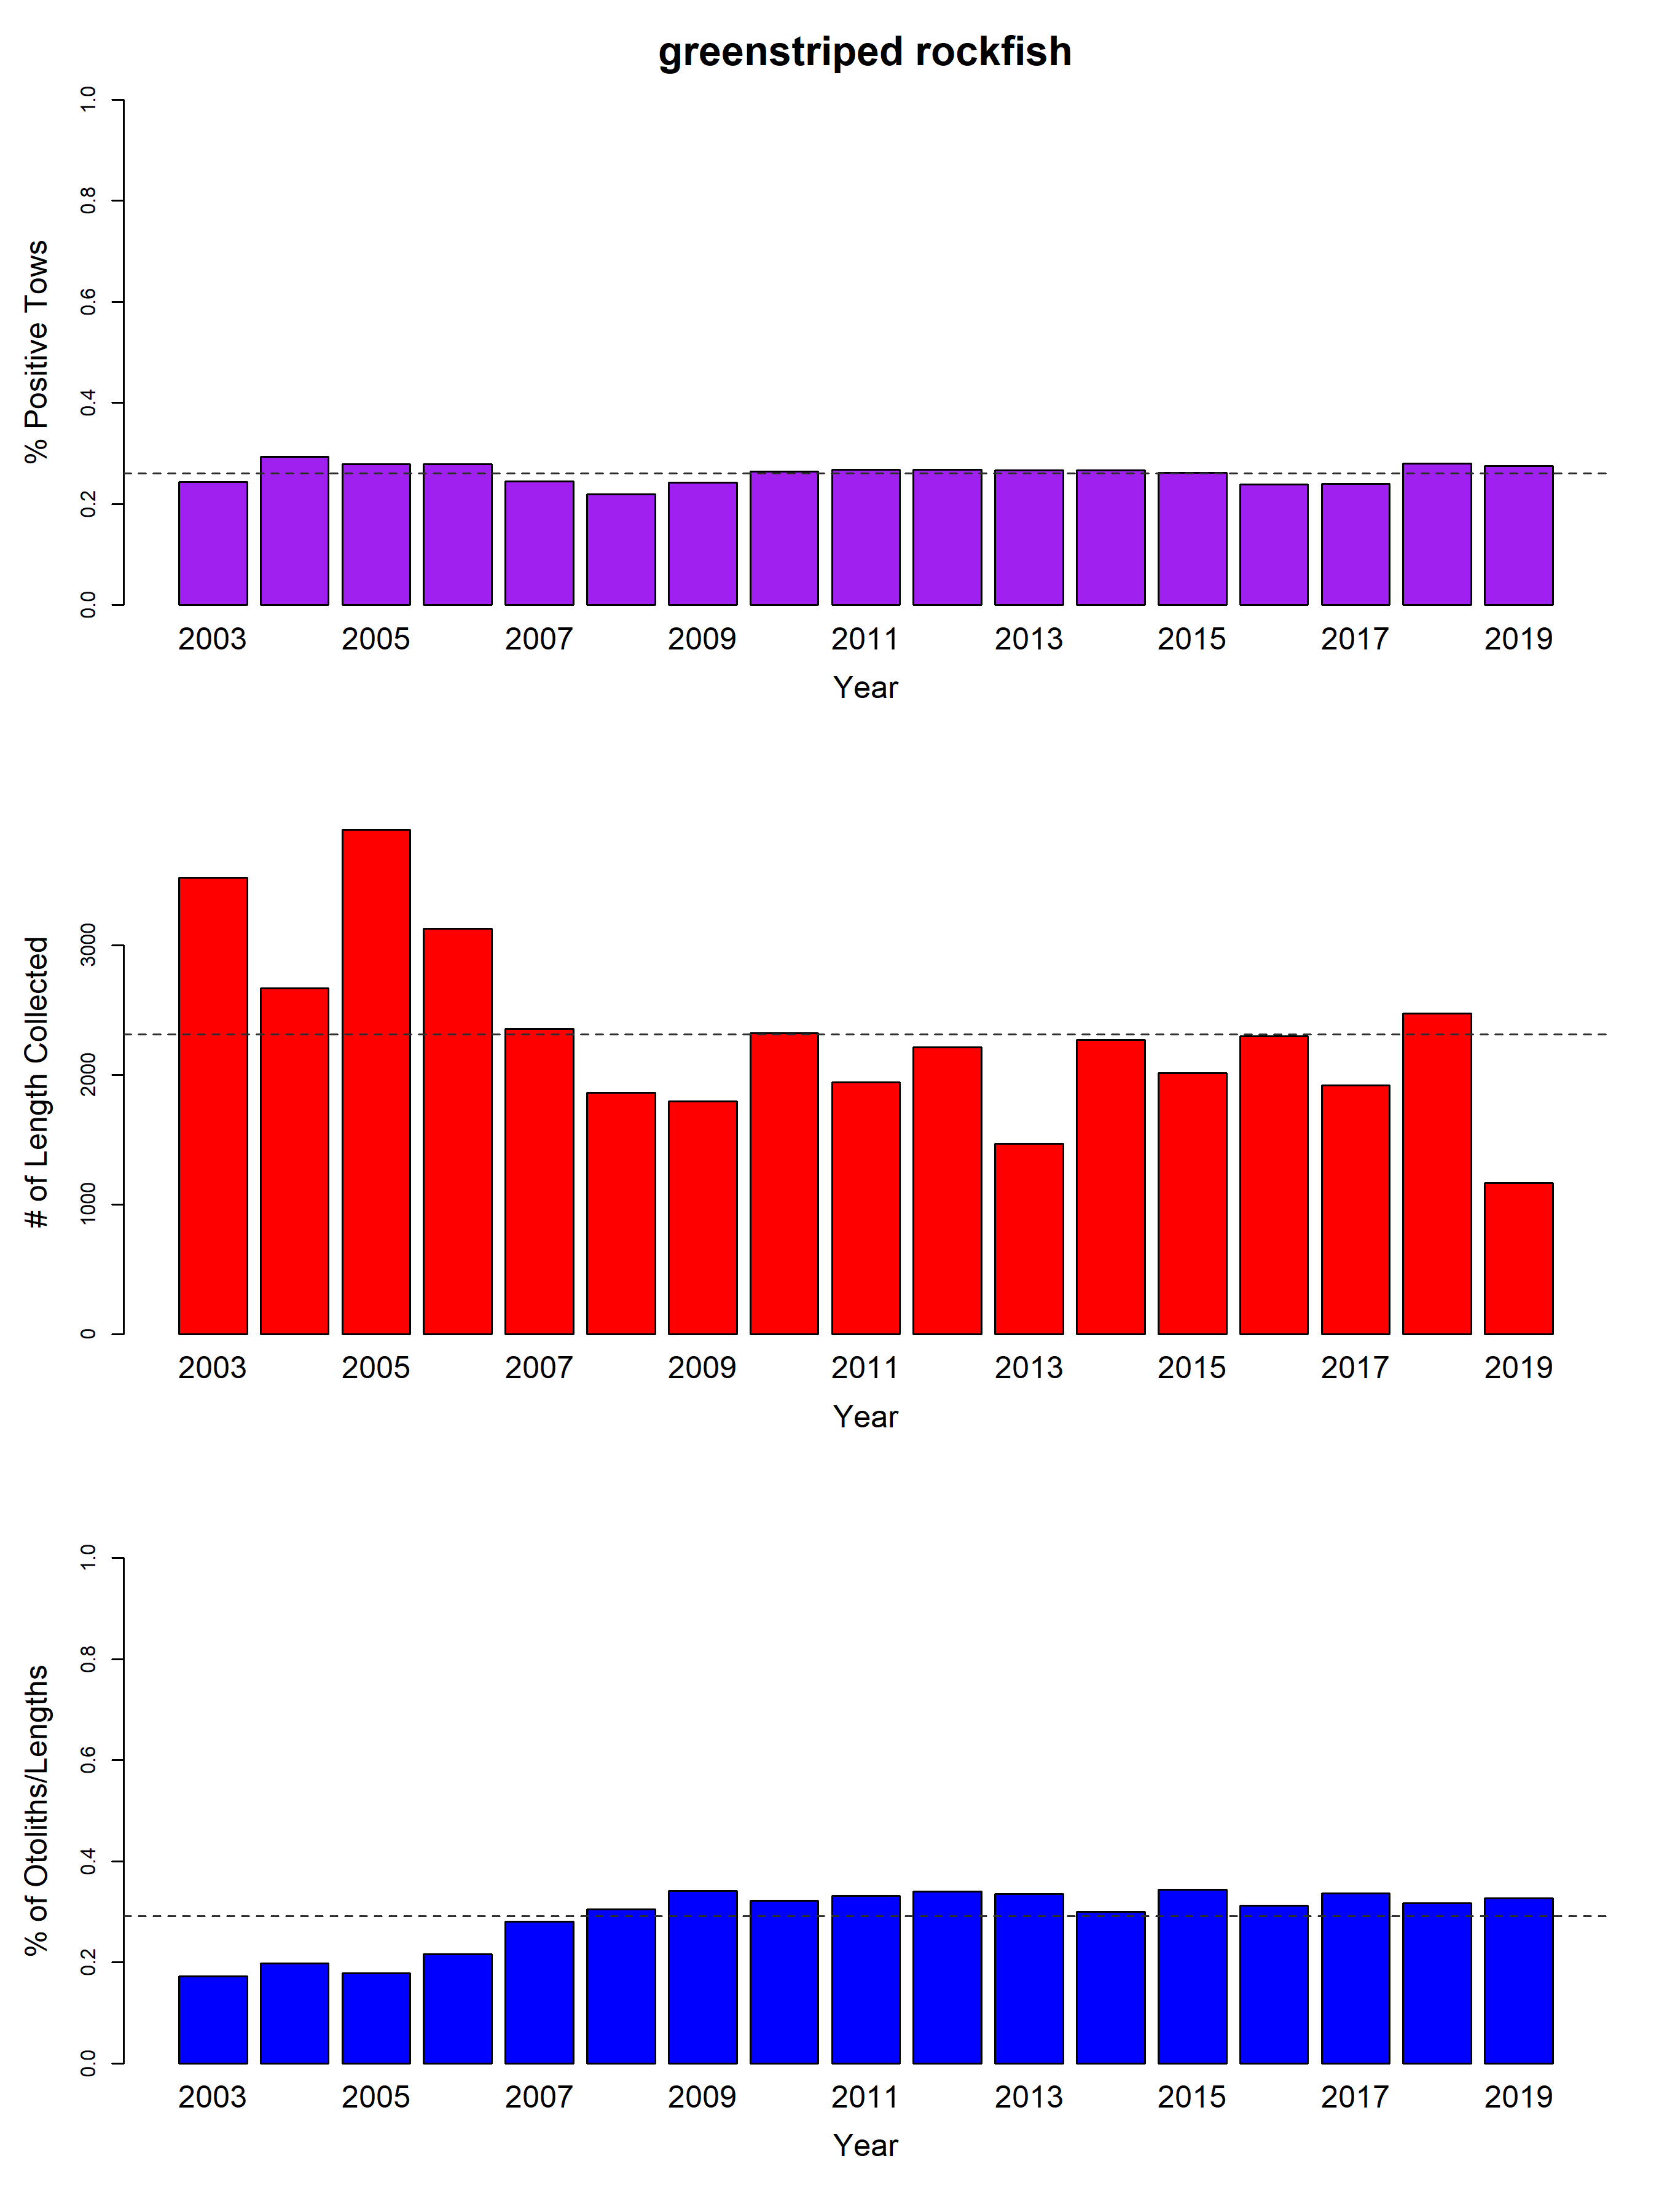
\includegraphics[width=0.6\textwidth,height=\textheight]{C:/Assessments/2020/survey_summary/sum_plots/greenstriped_rockfish_survey_stats.png}
\FloatBarrier  

\FloatBarrier

\FloatBarrier

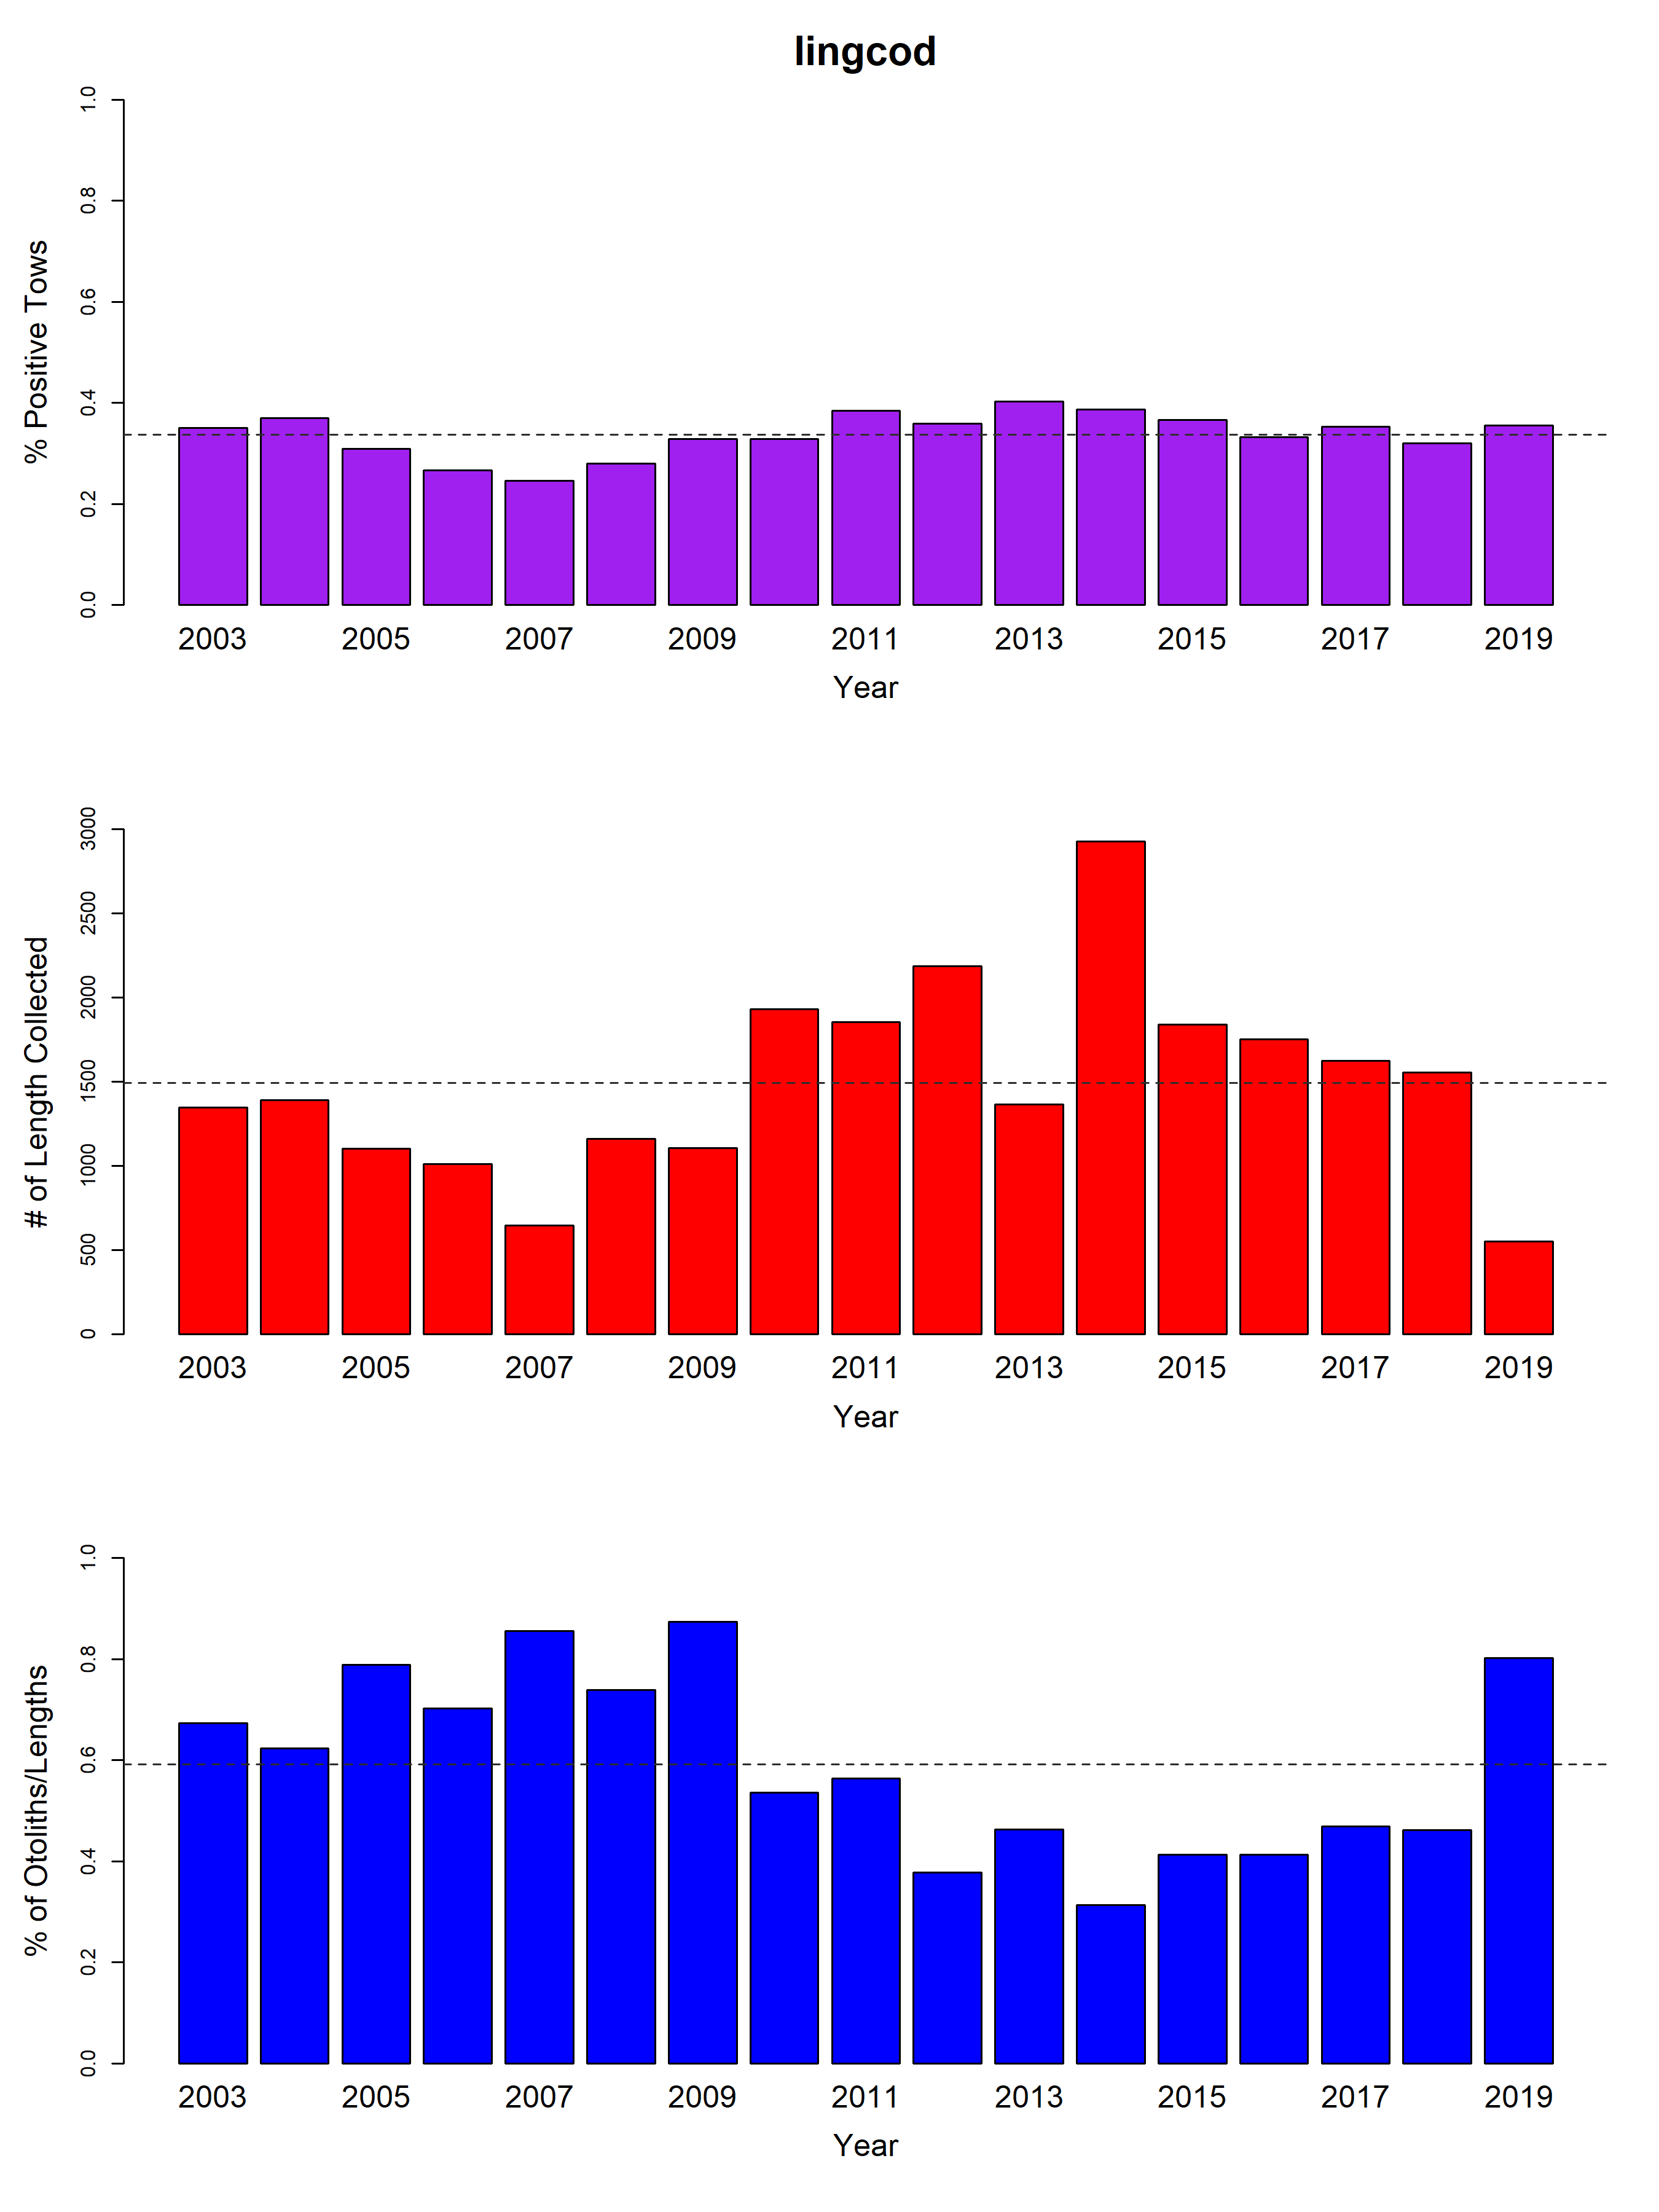
\includegraphics[width=0.6\textwidth,height=\textheight]{C:/Assessments/2020/survey_summary/sum_plots/lingcod_survey_stats.png}
\FloatBarrier  

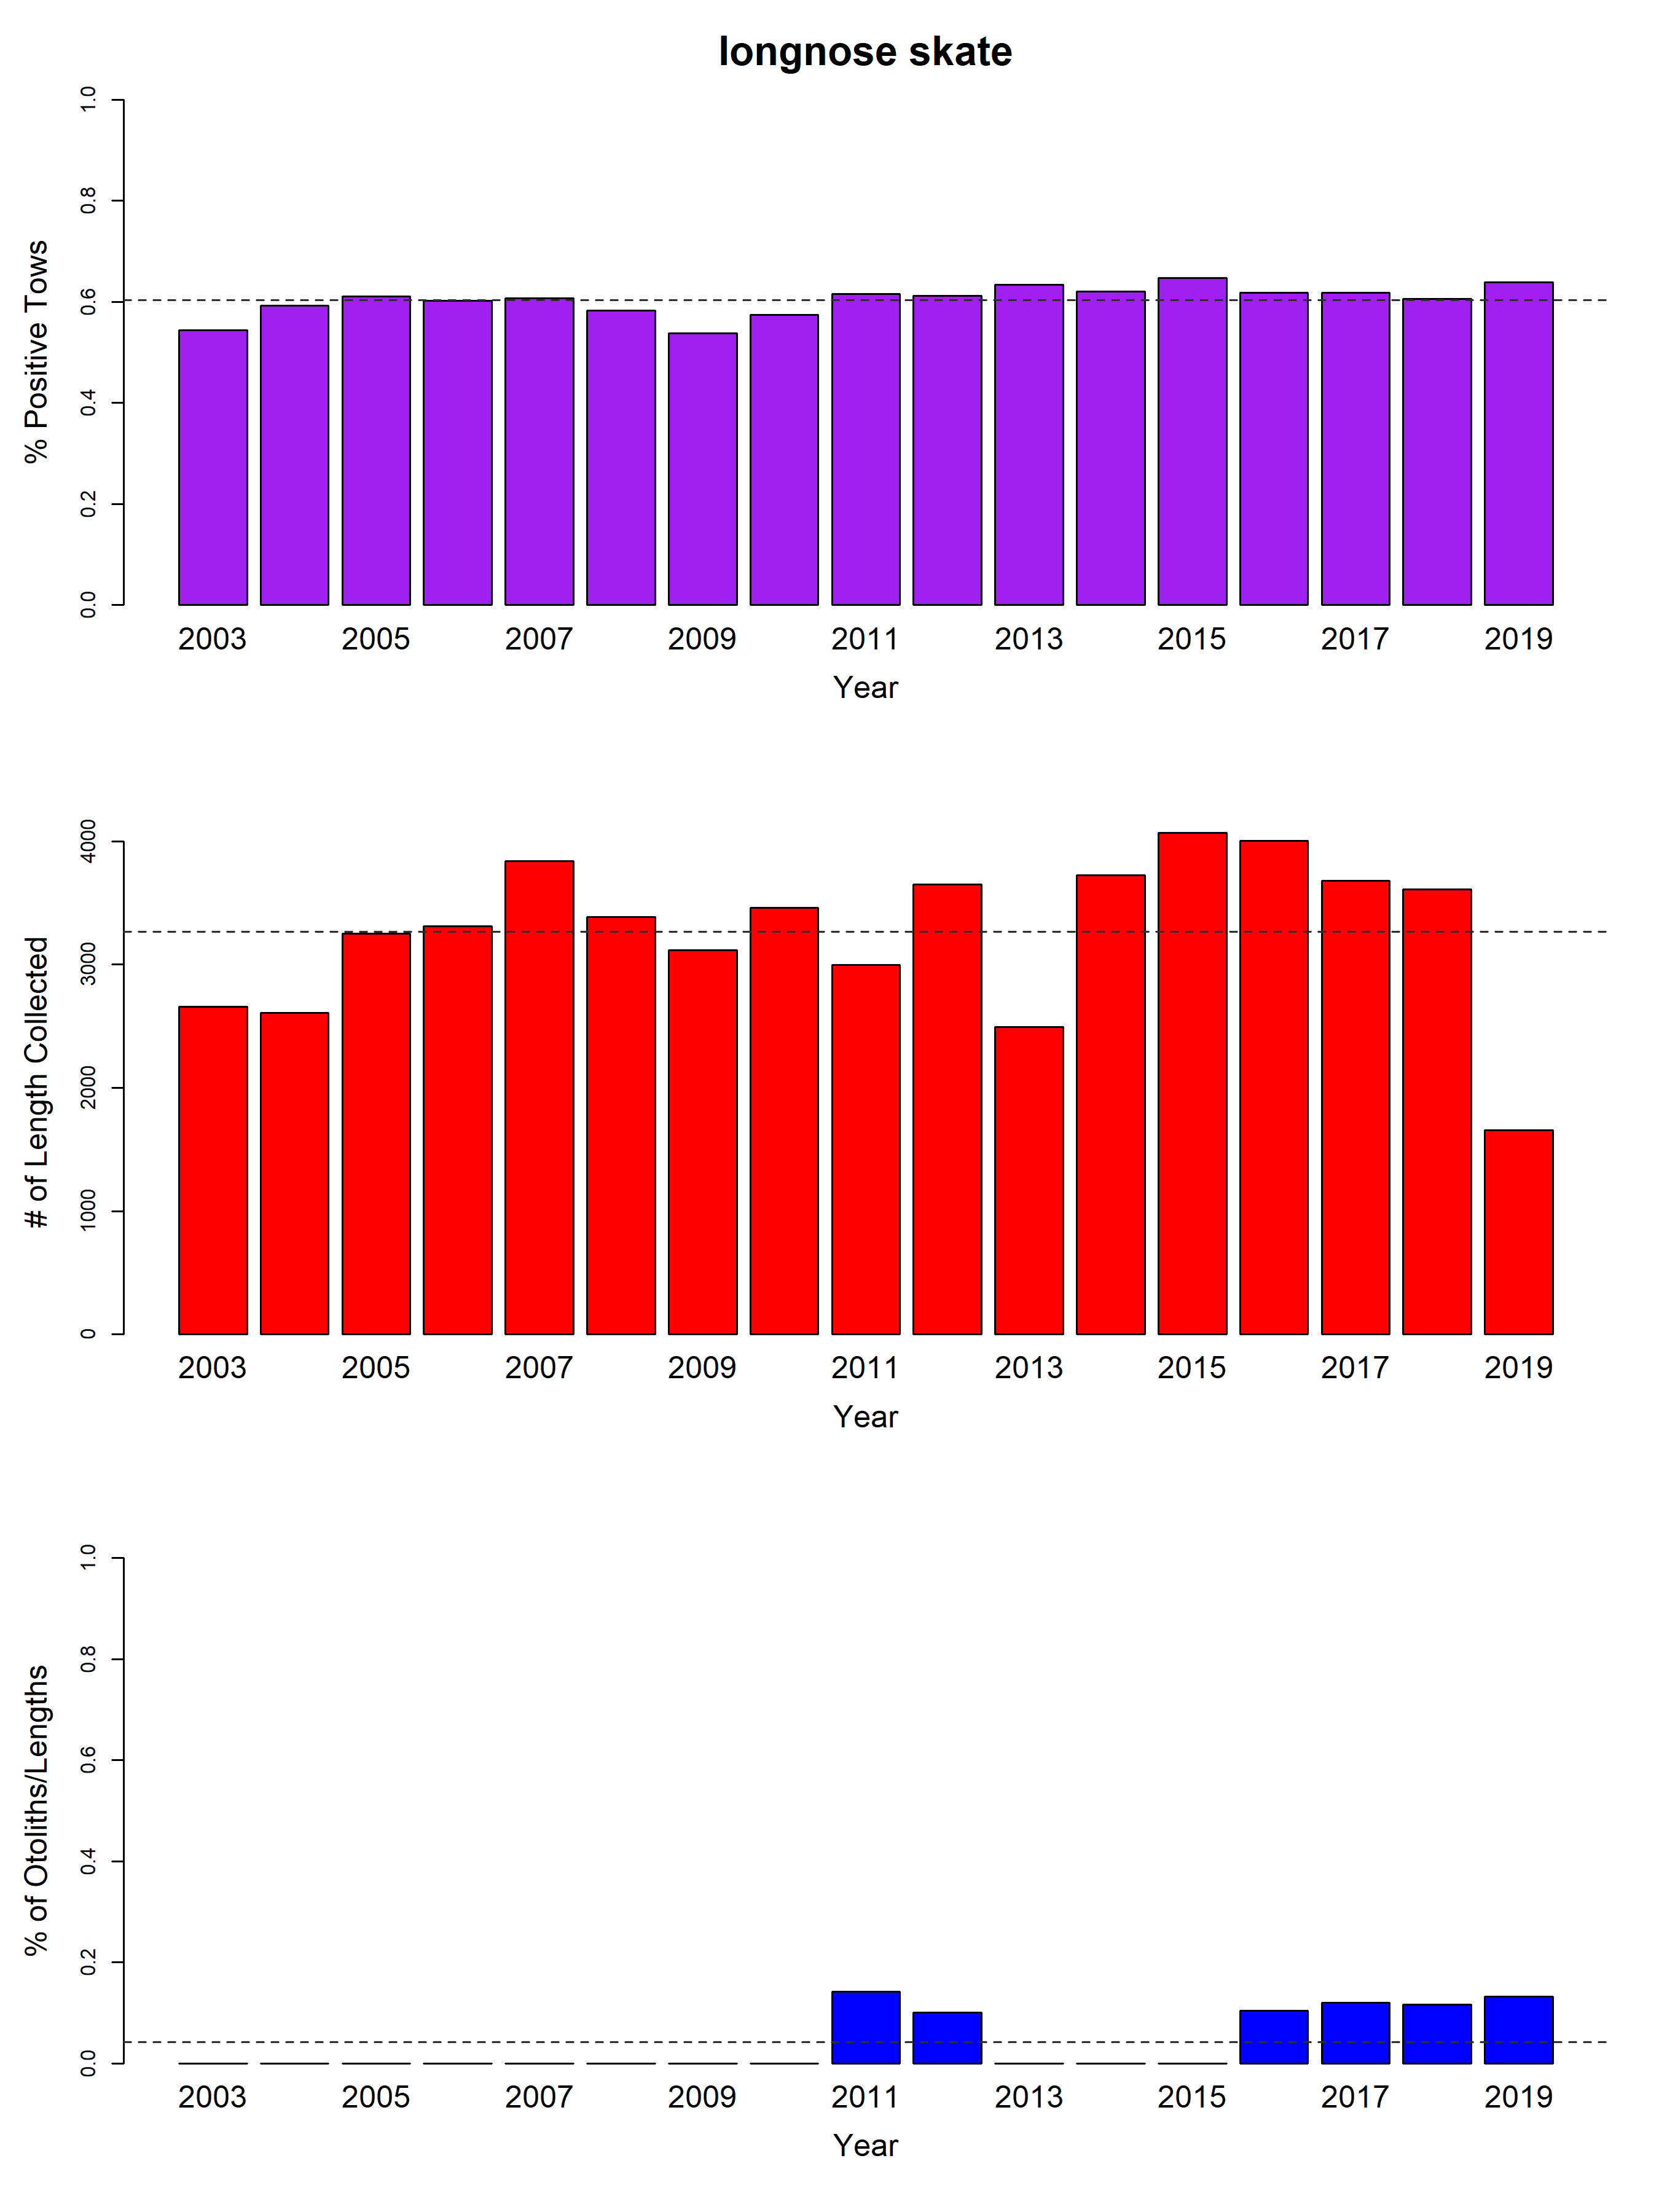
\includegraphics[width=0.6\textwidth,height=\textheight]{C:/Assessments/2020/survey_summary/sum_plots/longnose_skate_survey_stats.png}
\FloatBarrier  

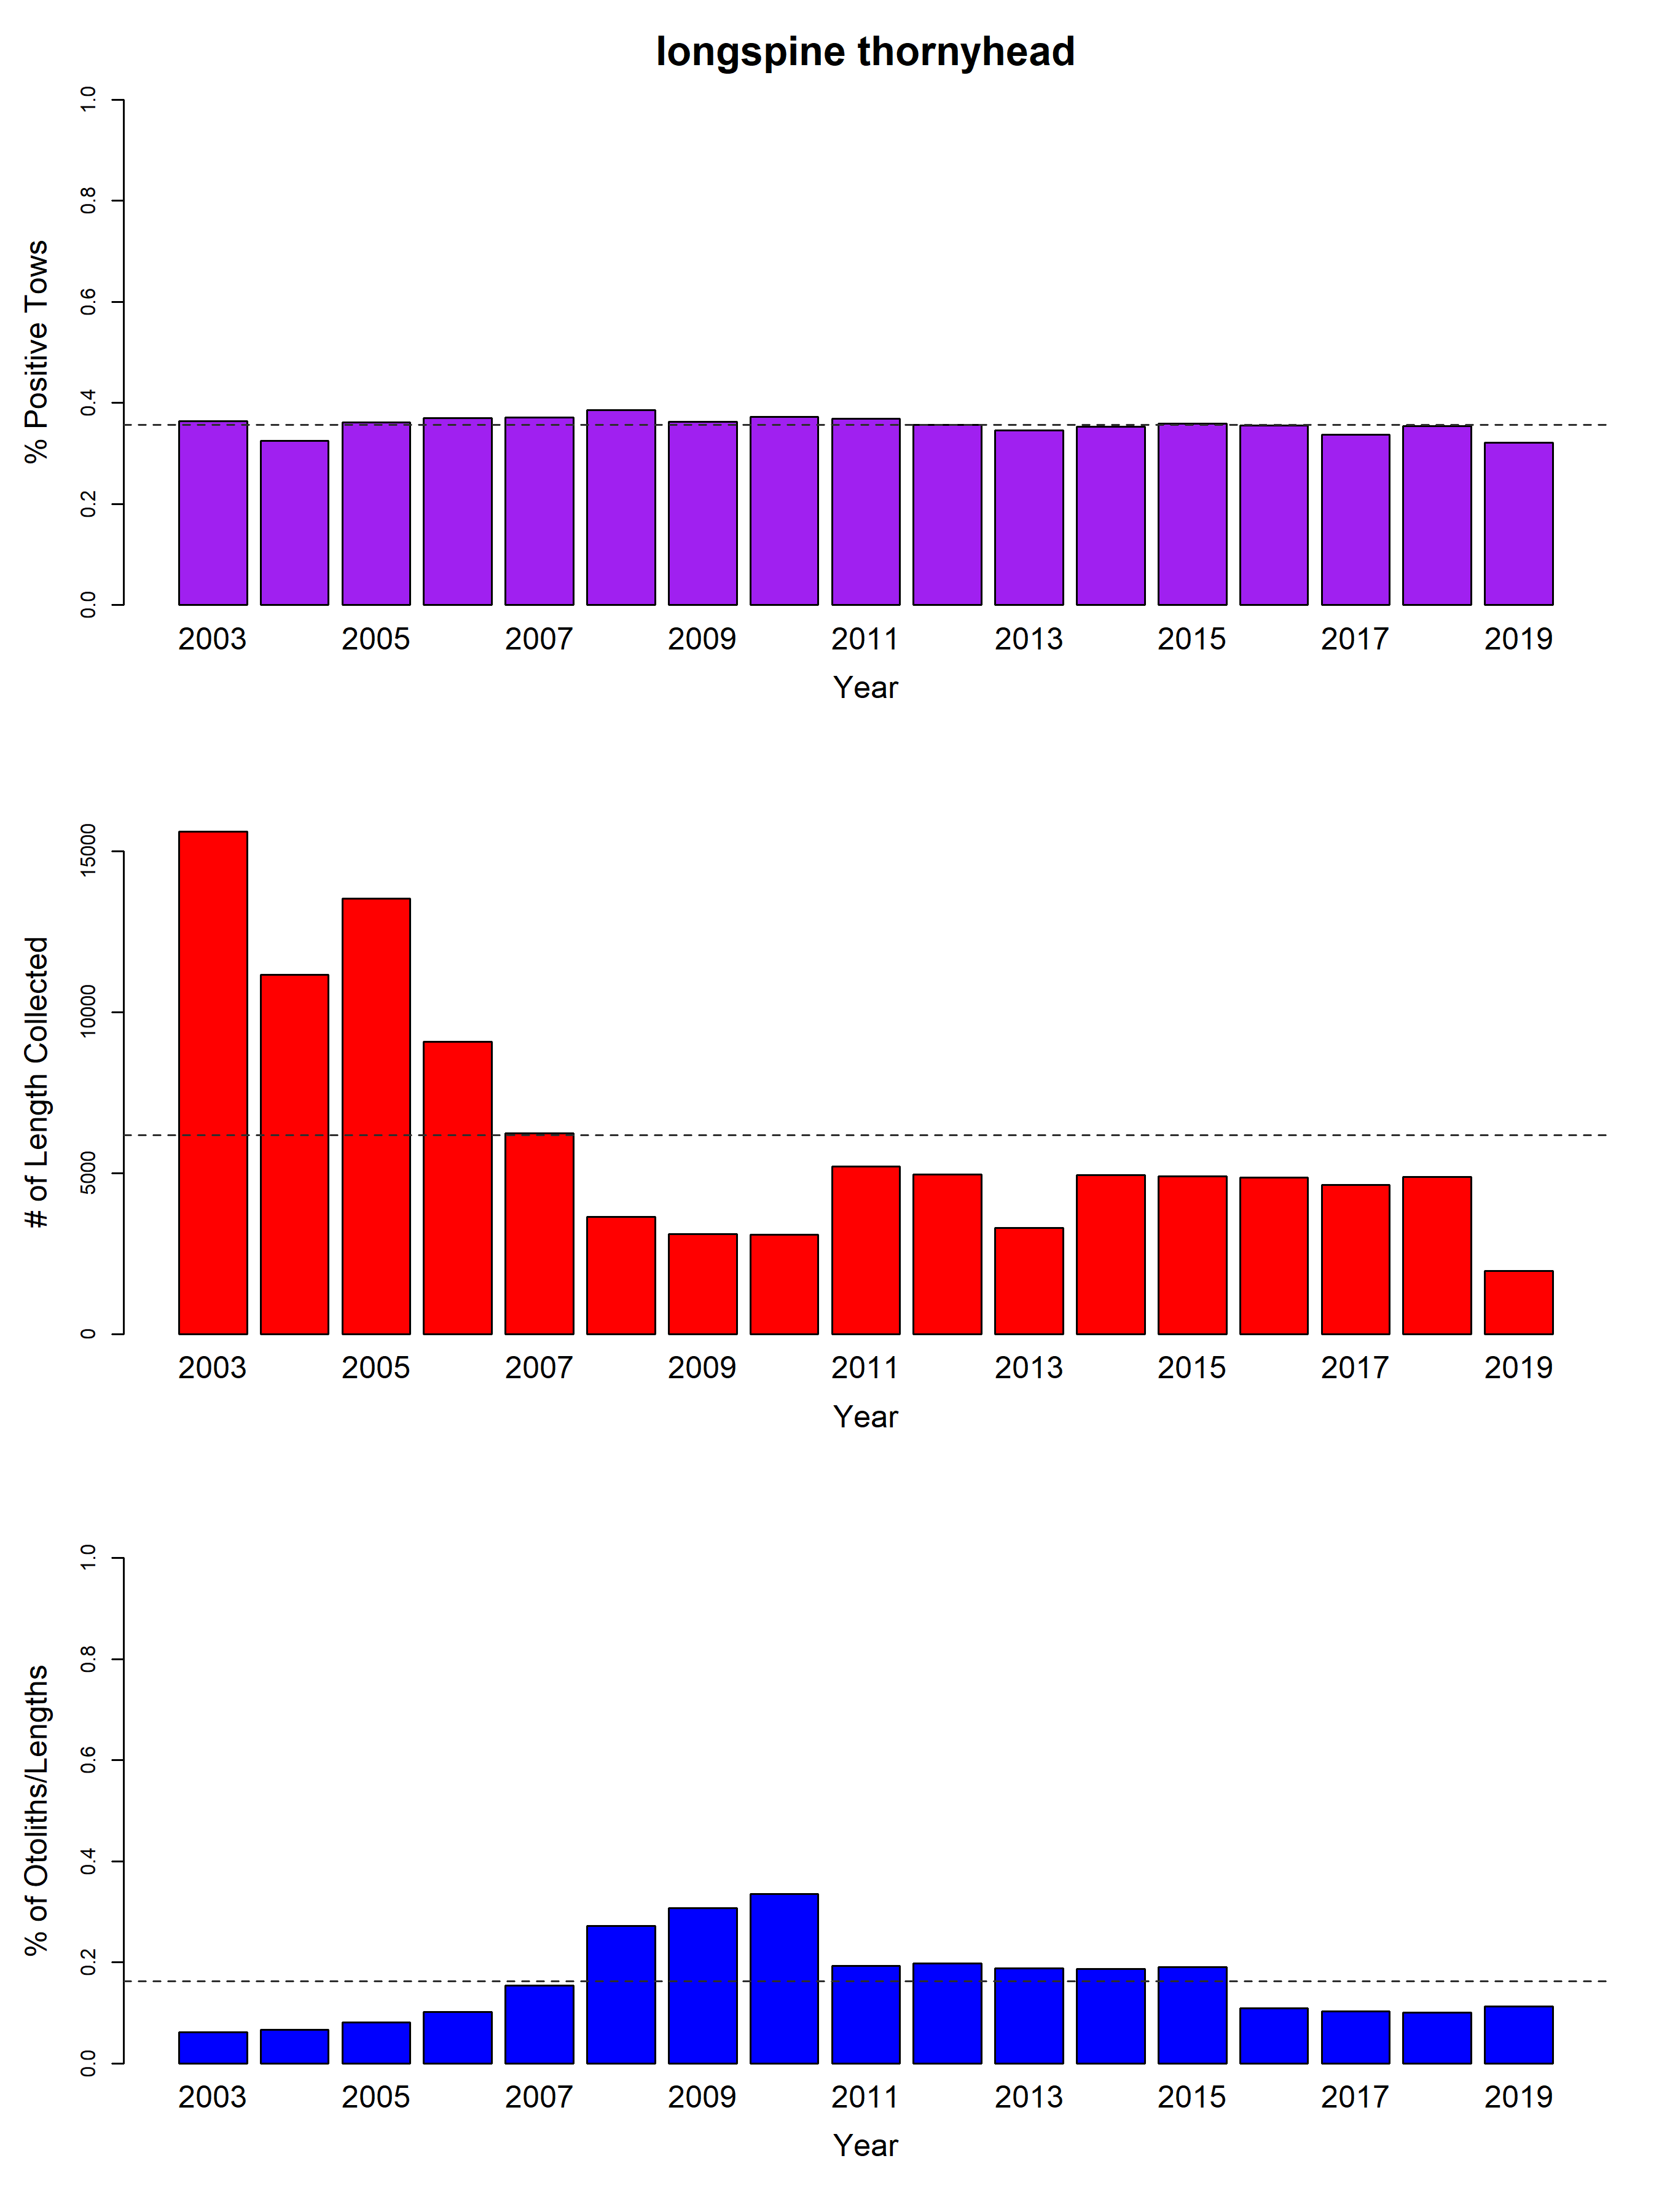
\includegraphics[width=0.6\textwidth,height=\textheight]{C:/Assessments/2020/survey_summary/sum_plots/longspine_thornyhead_survey_stats.png}
\FloatBarrier  

\FloatBarrier

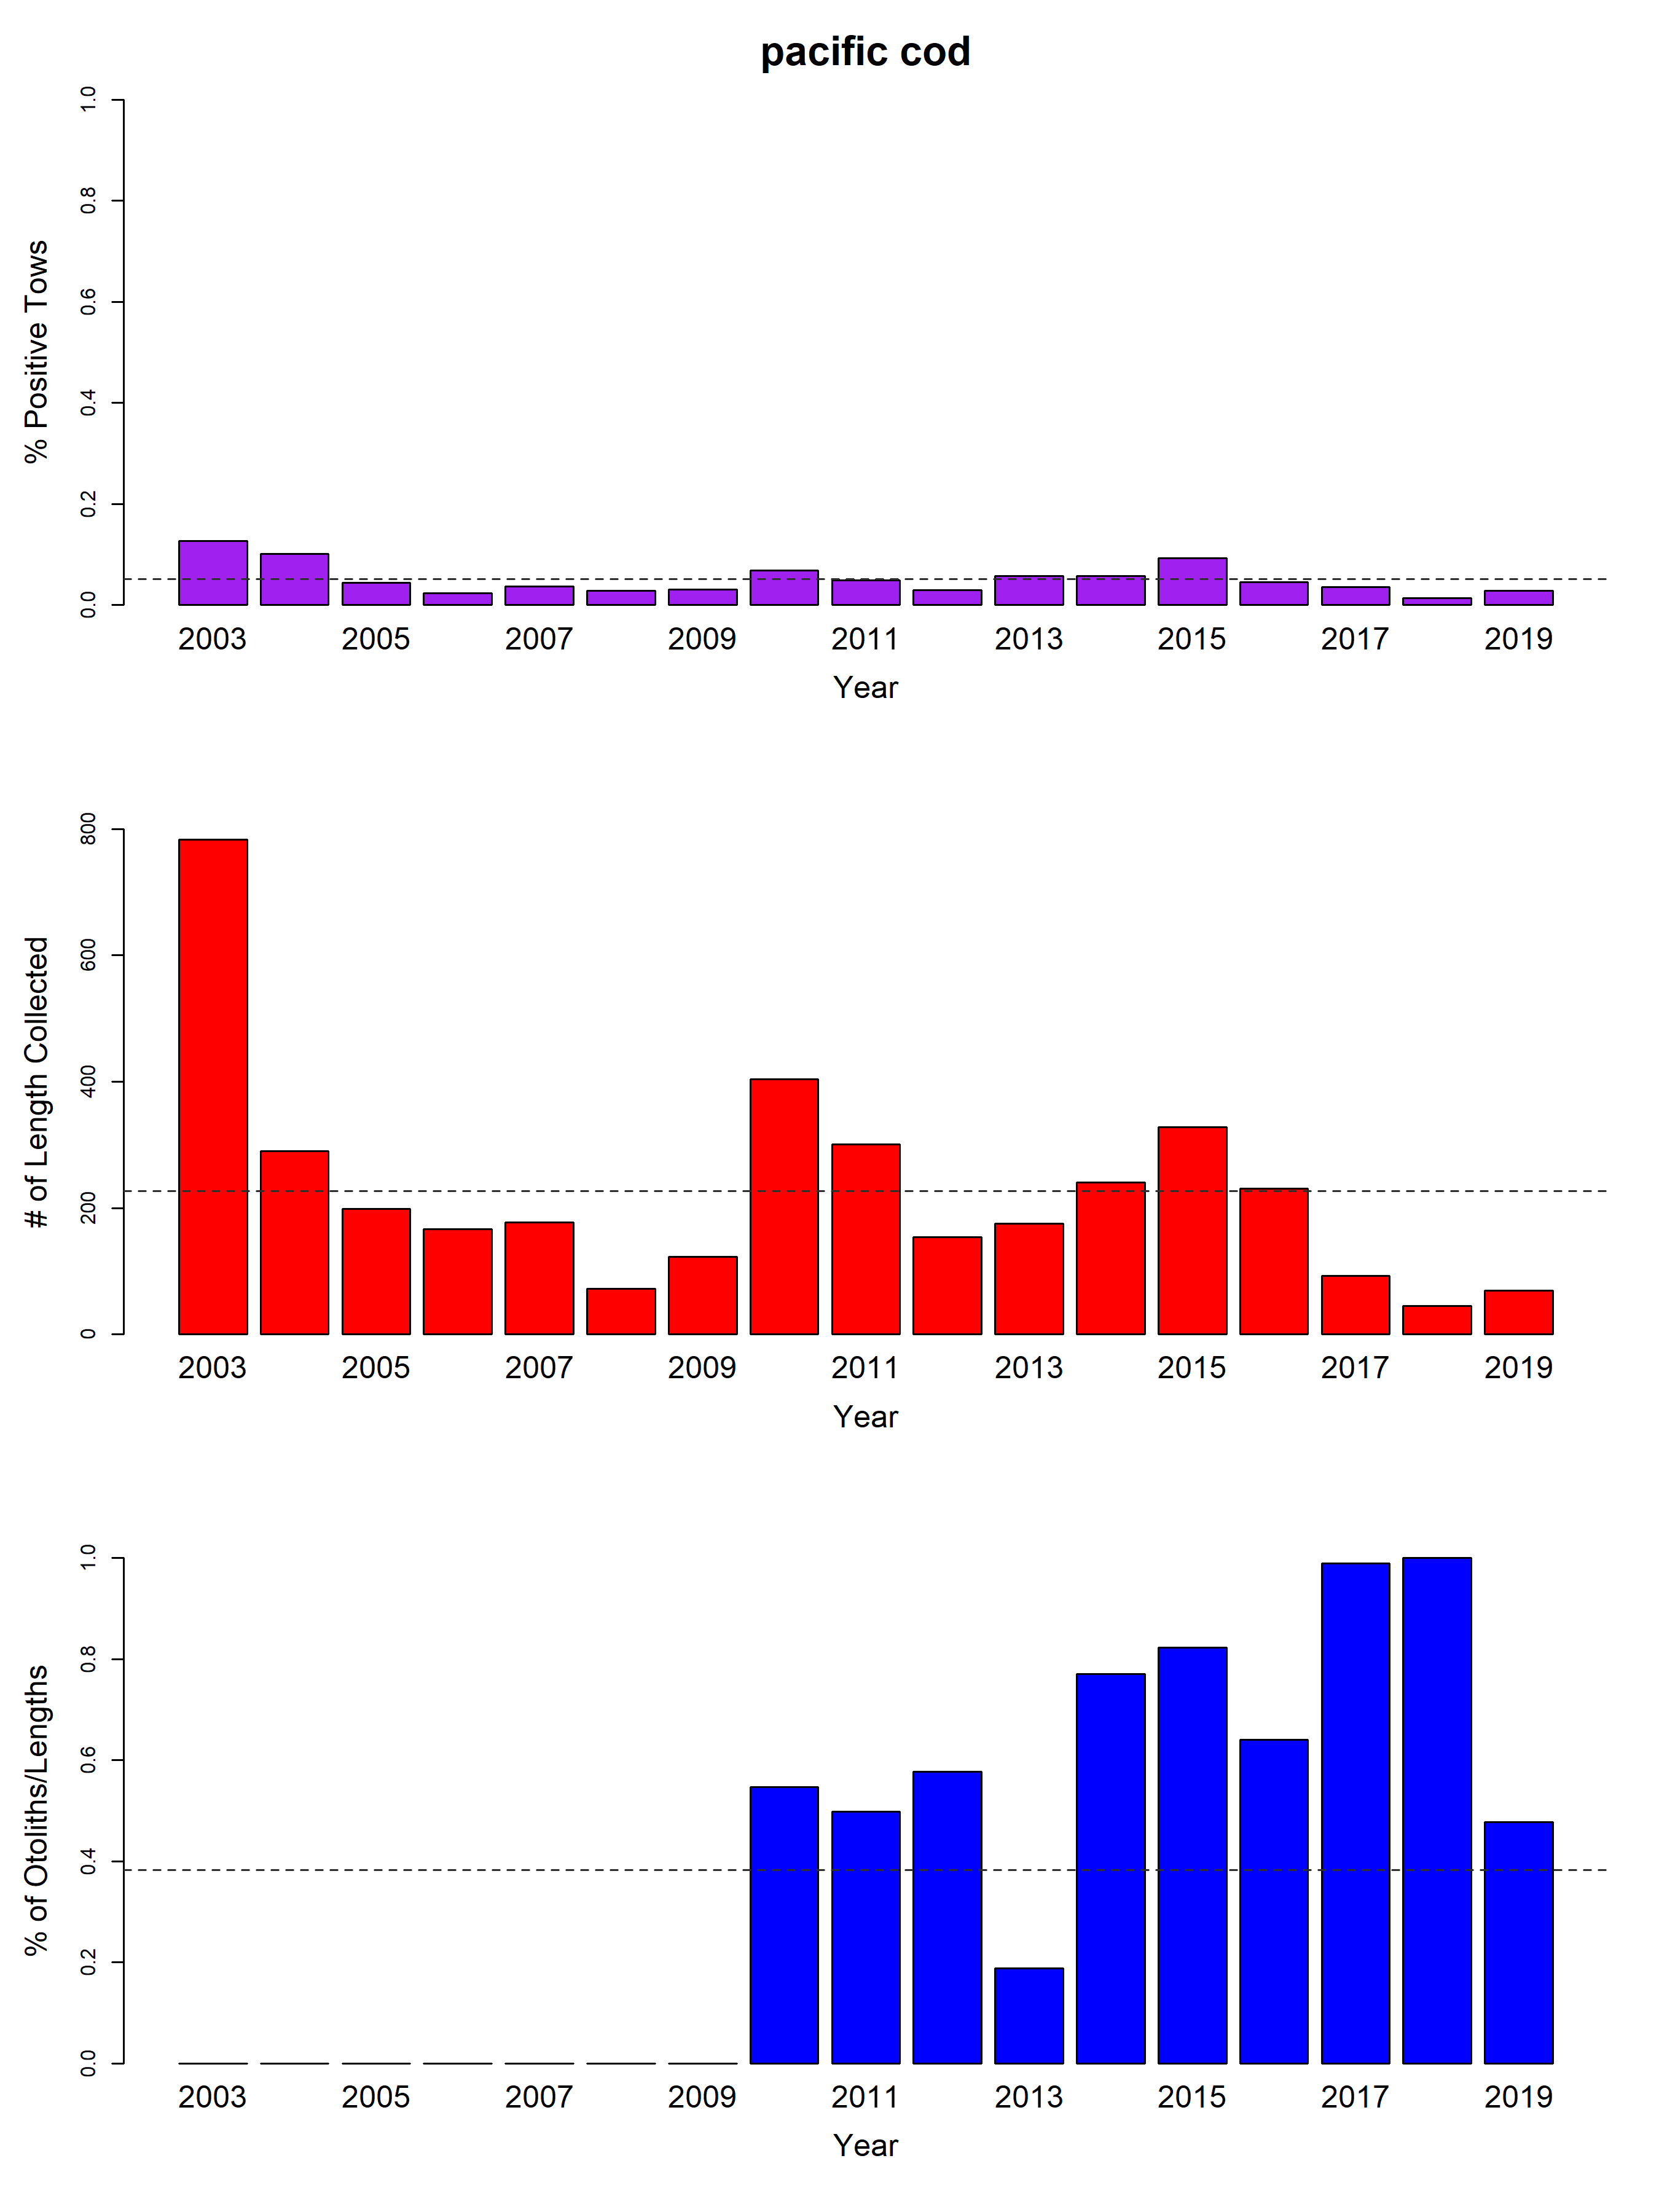
\includegraphics[width=0.6\textwidth,height=\textheight]{C:/Assessments/2020/survey_summary/sum_plots/pacific_cod_survey_stats.png}
\FloatBarrier  

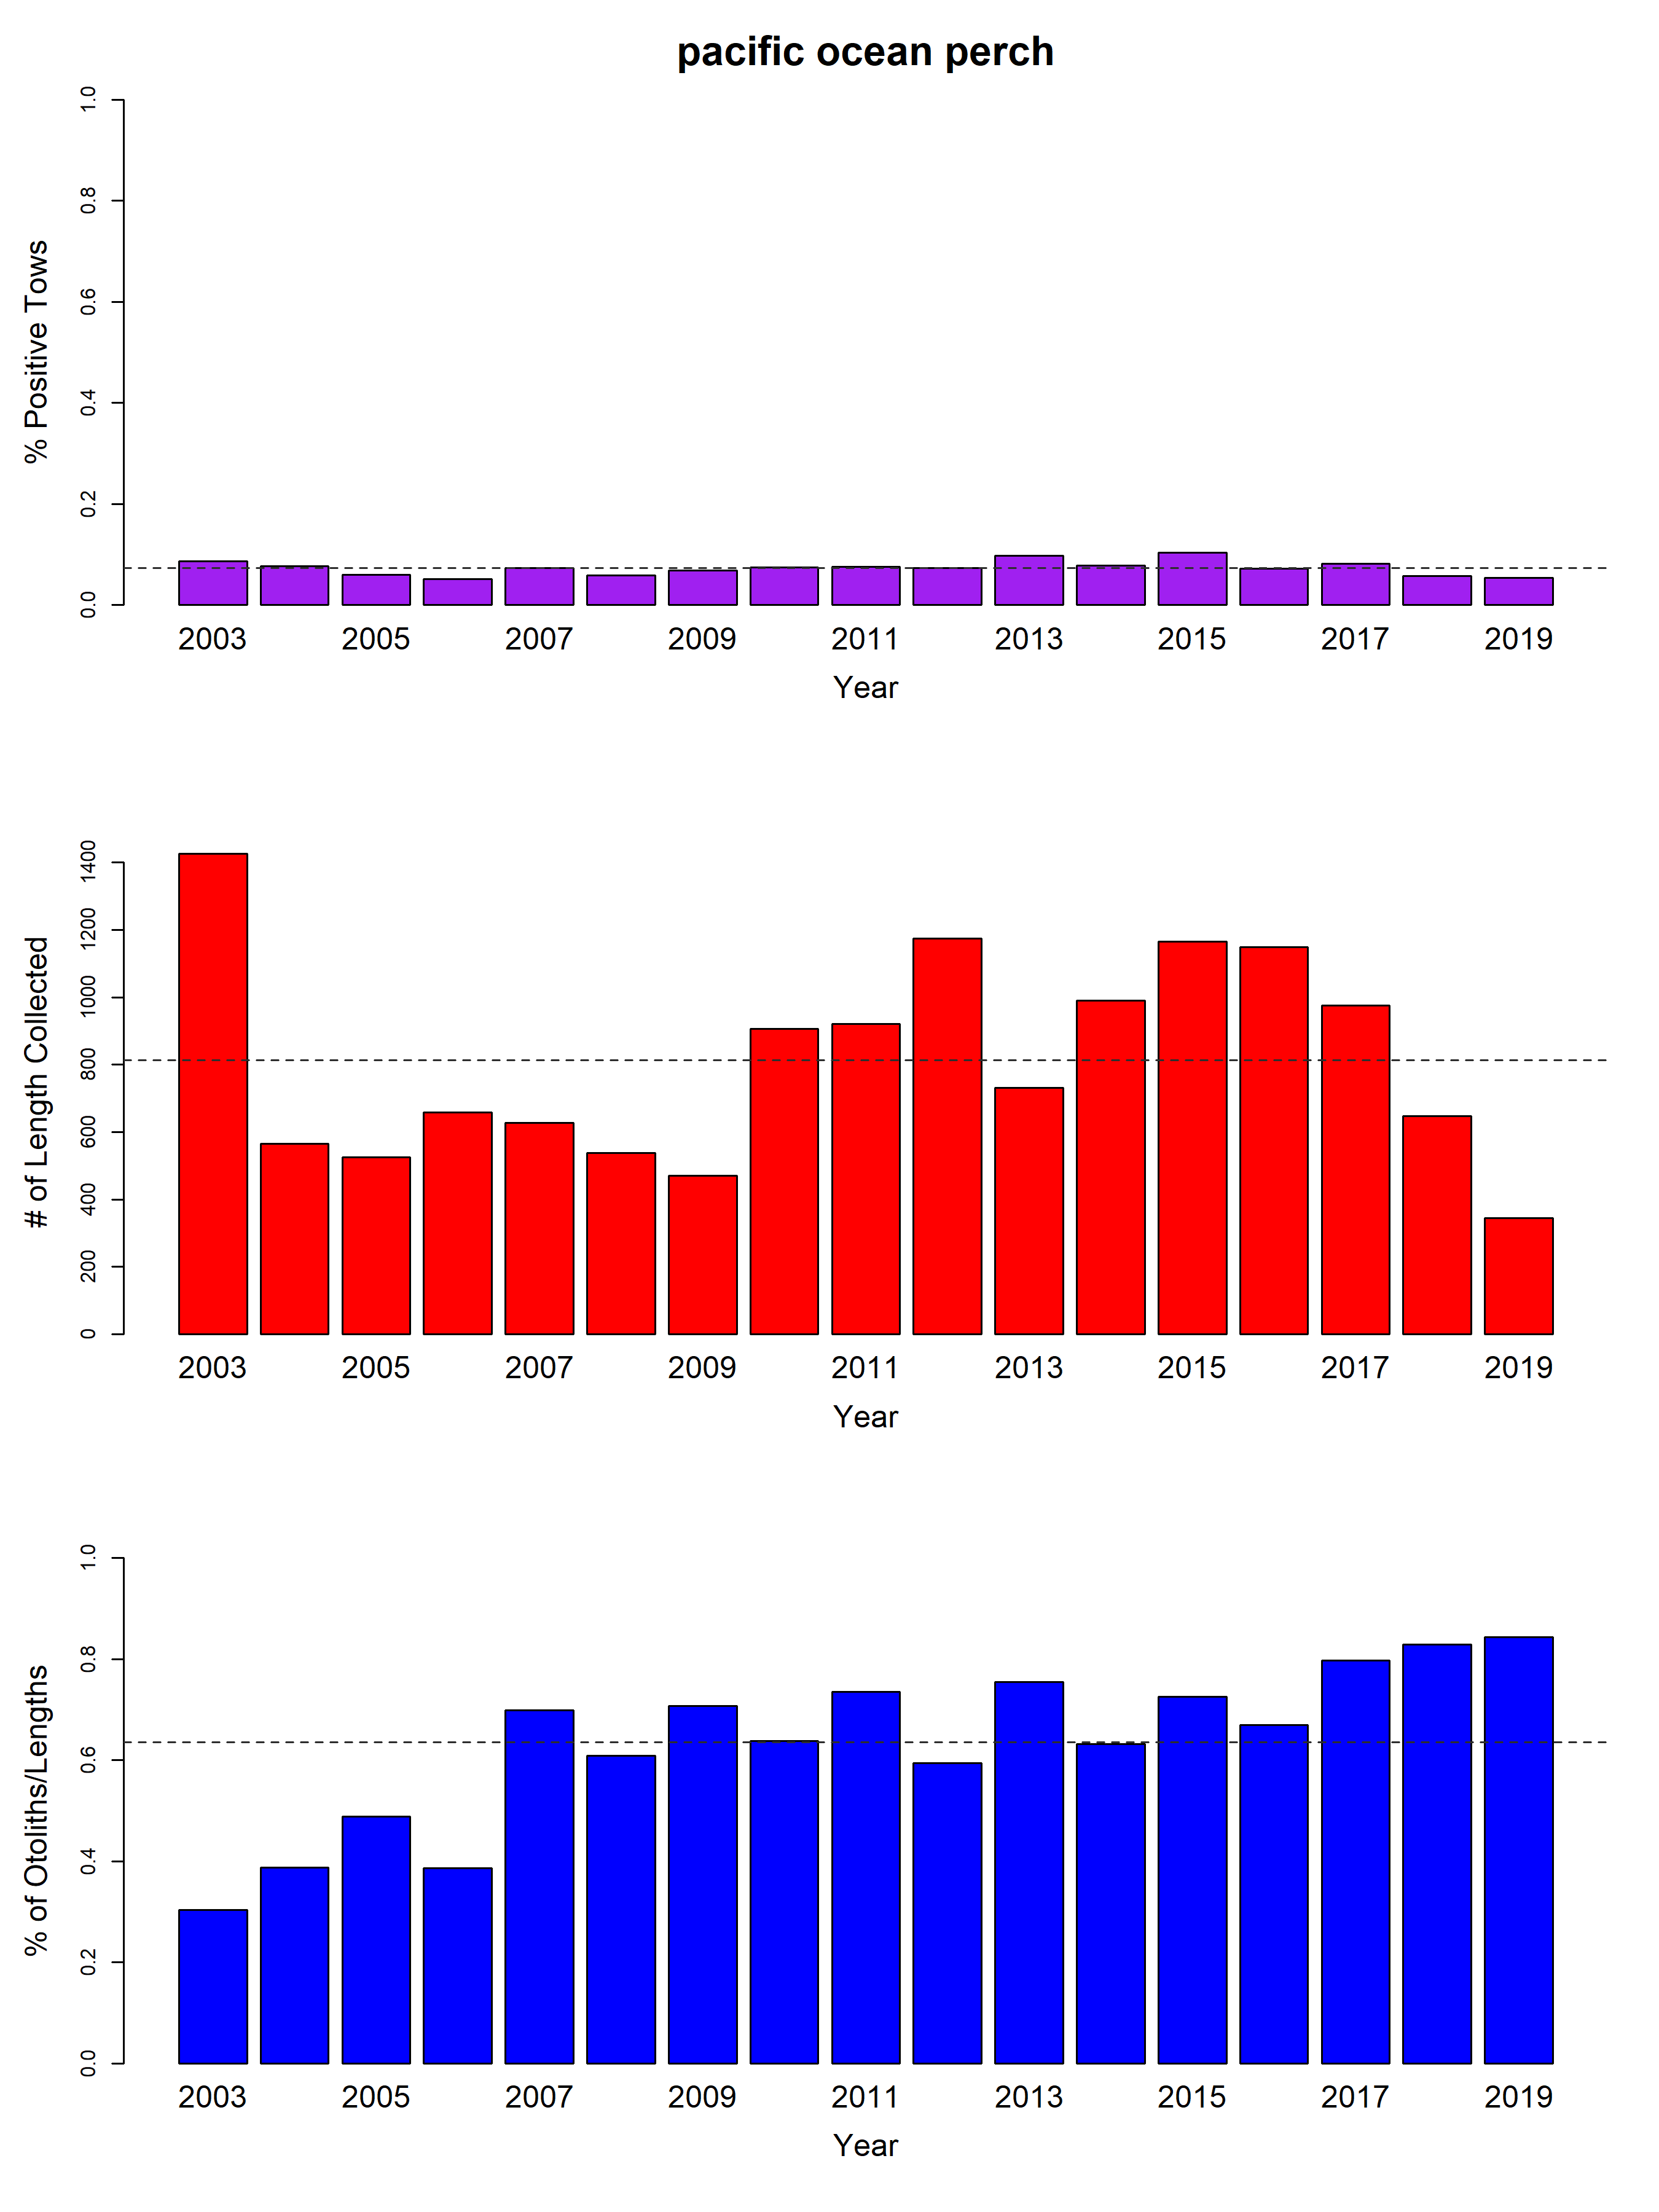
\includegraphics[width=0.6\textwidth,height=\textheight]{C:/Assessments/2020/survey_summary/sum_plots/pacific_ocean_perch_survey_stats.png}
\FloatBarrier  

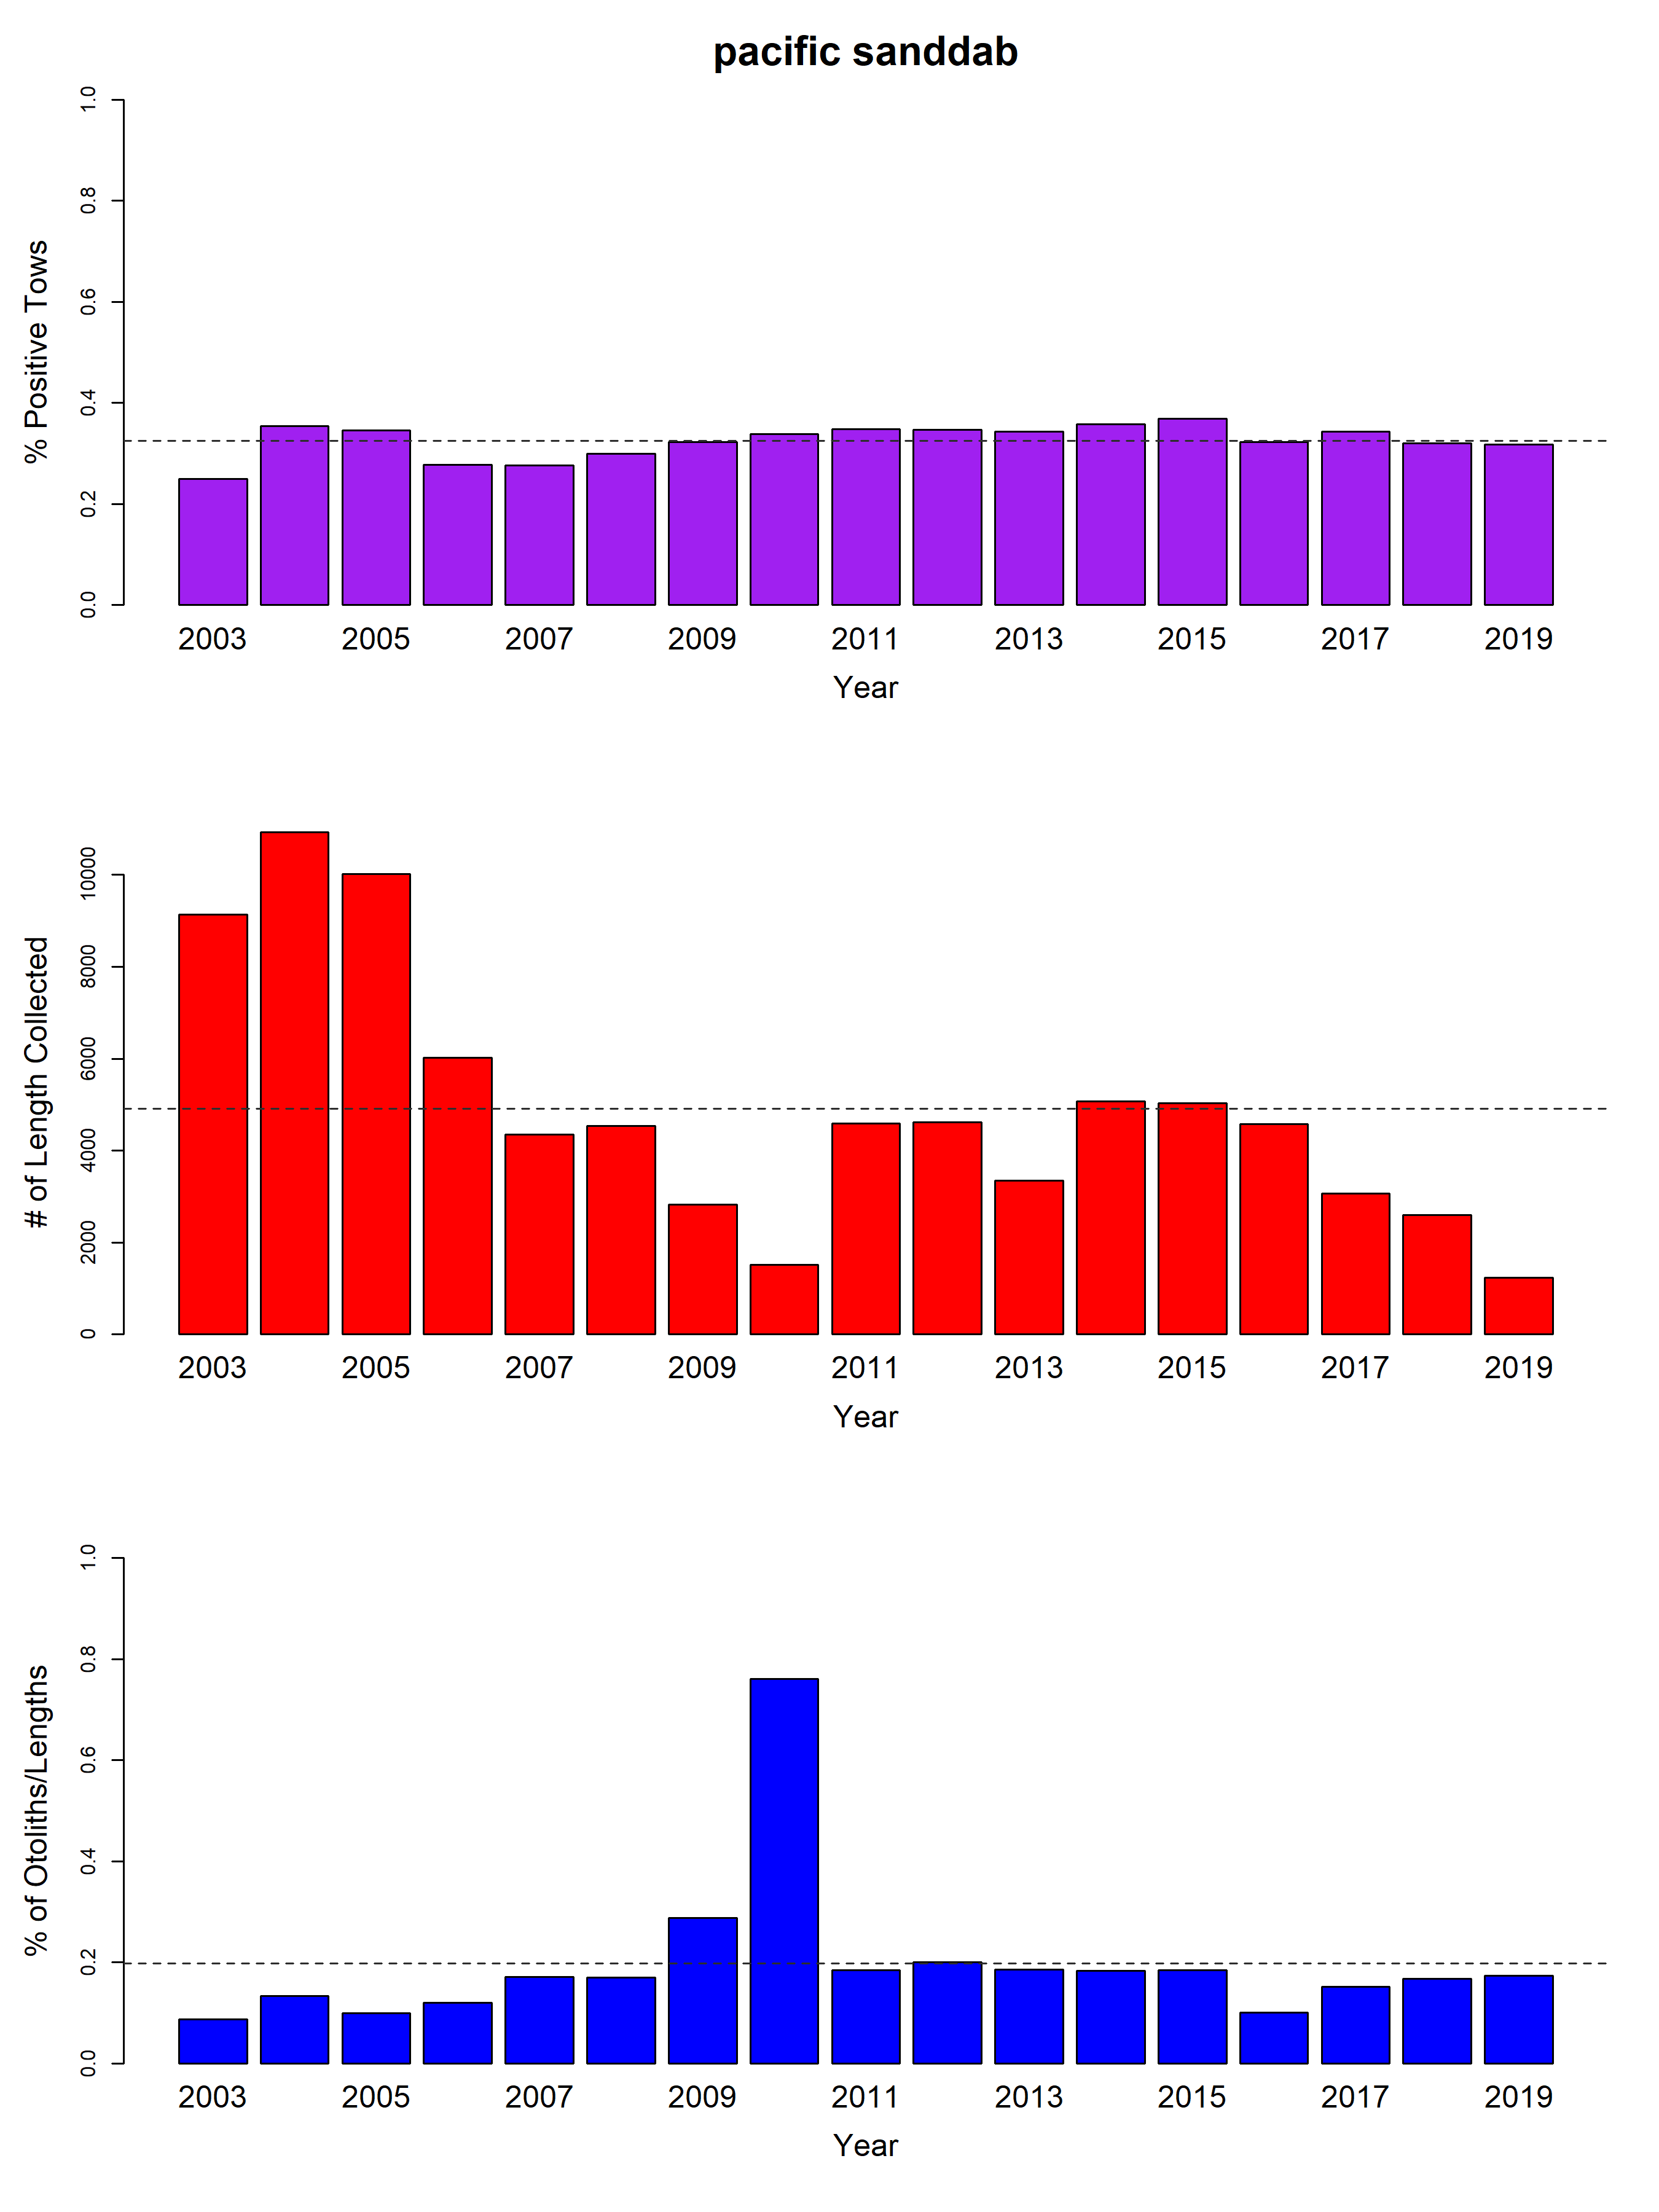
\includegraphics[width=0.6\textwidth,height=\textheight]{C:/Assessments/2020/survey_summary/sum_plots/pacific_sanddab_survey_stats.png}
\FloatBarrier  

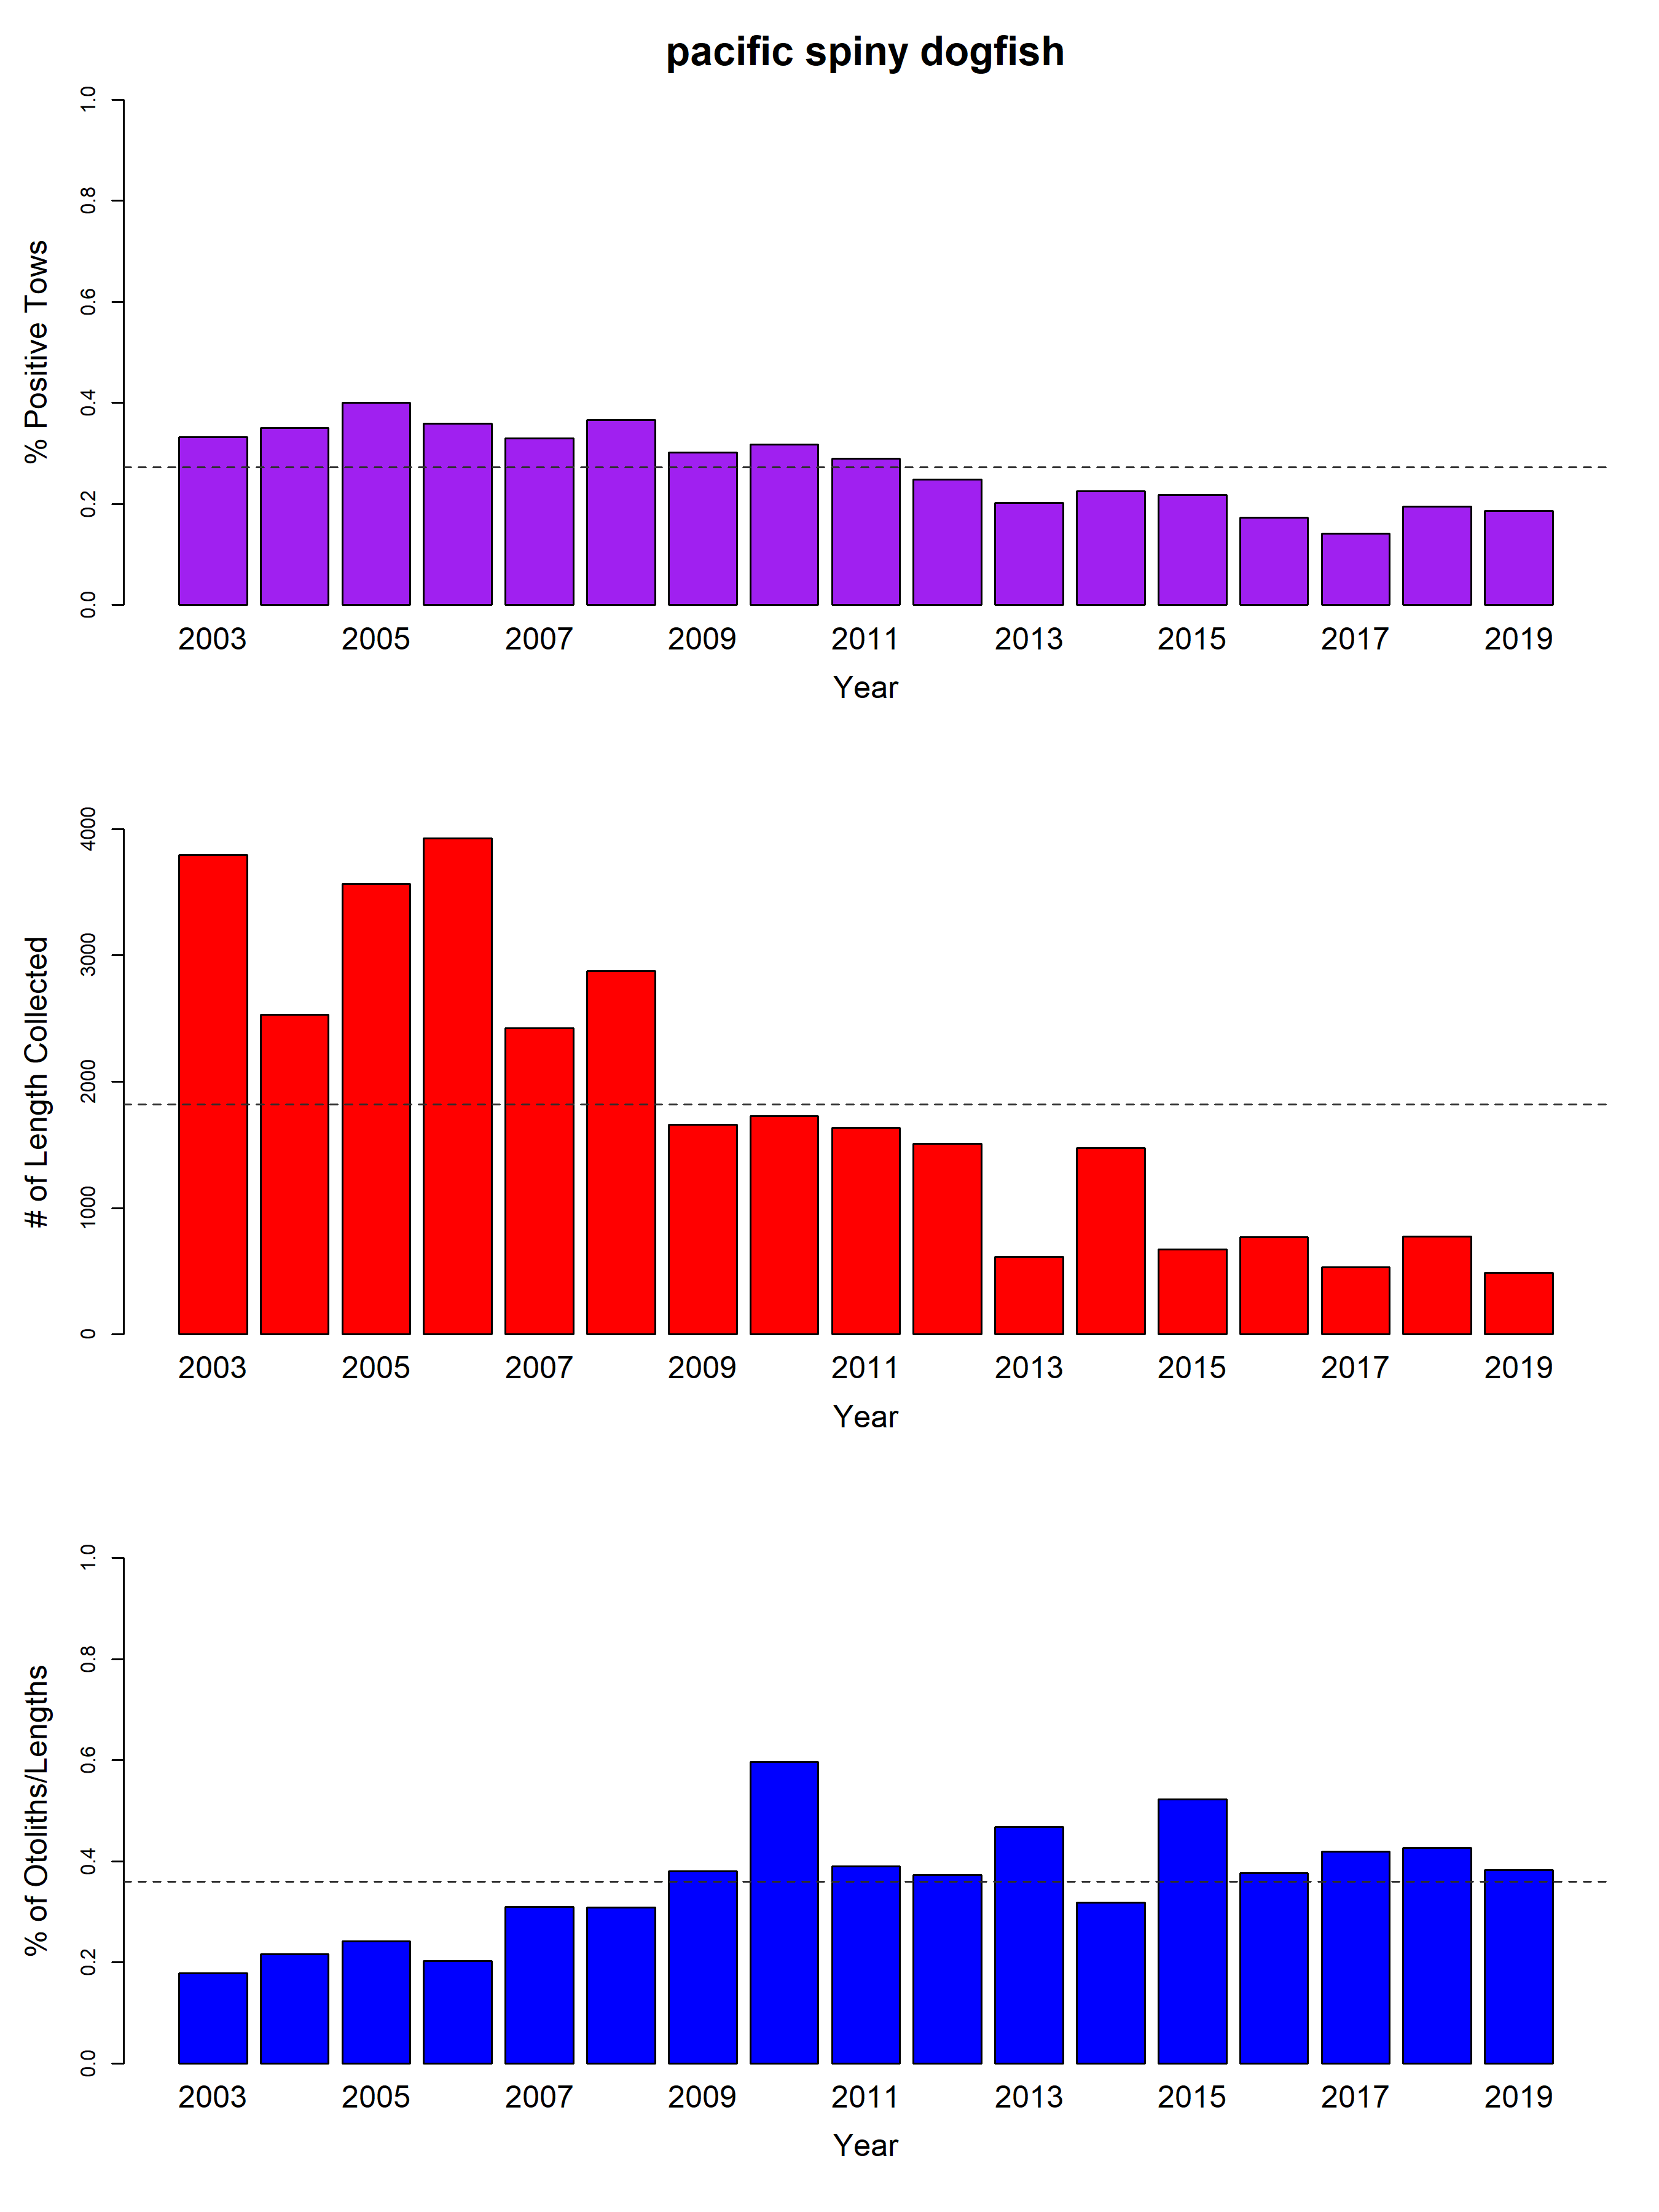
\includegraphics[width=0.6\textwidth,height=\textheight]{C:/Assessments/2020/survey_summary/sum_plots/pacific_spiny_dogfish_survey_stats.png}
\FloatBarrier  

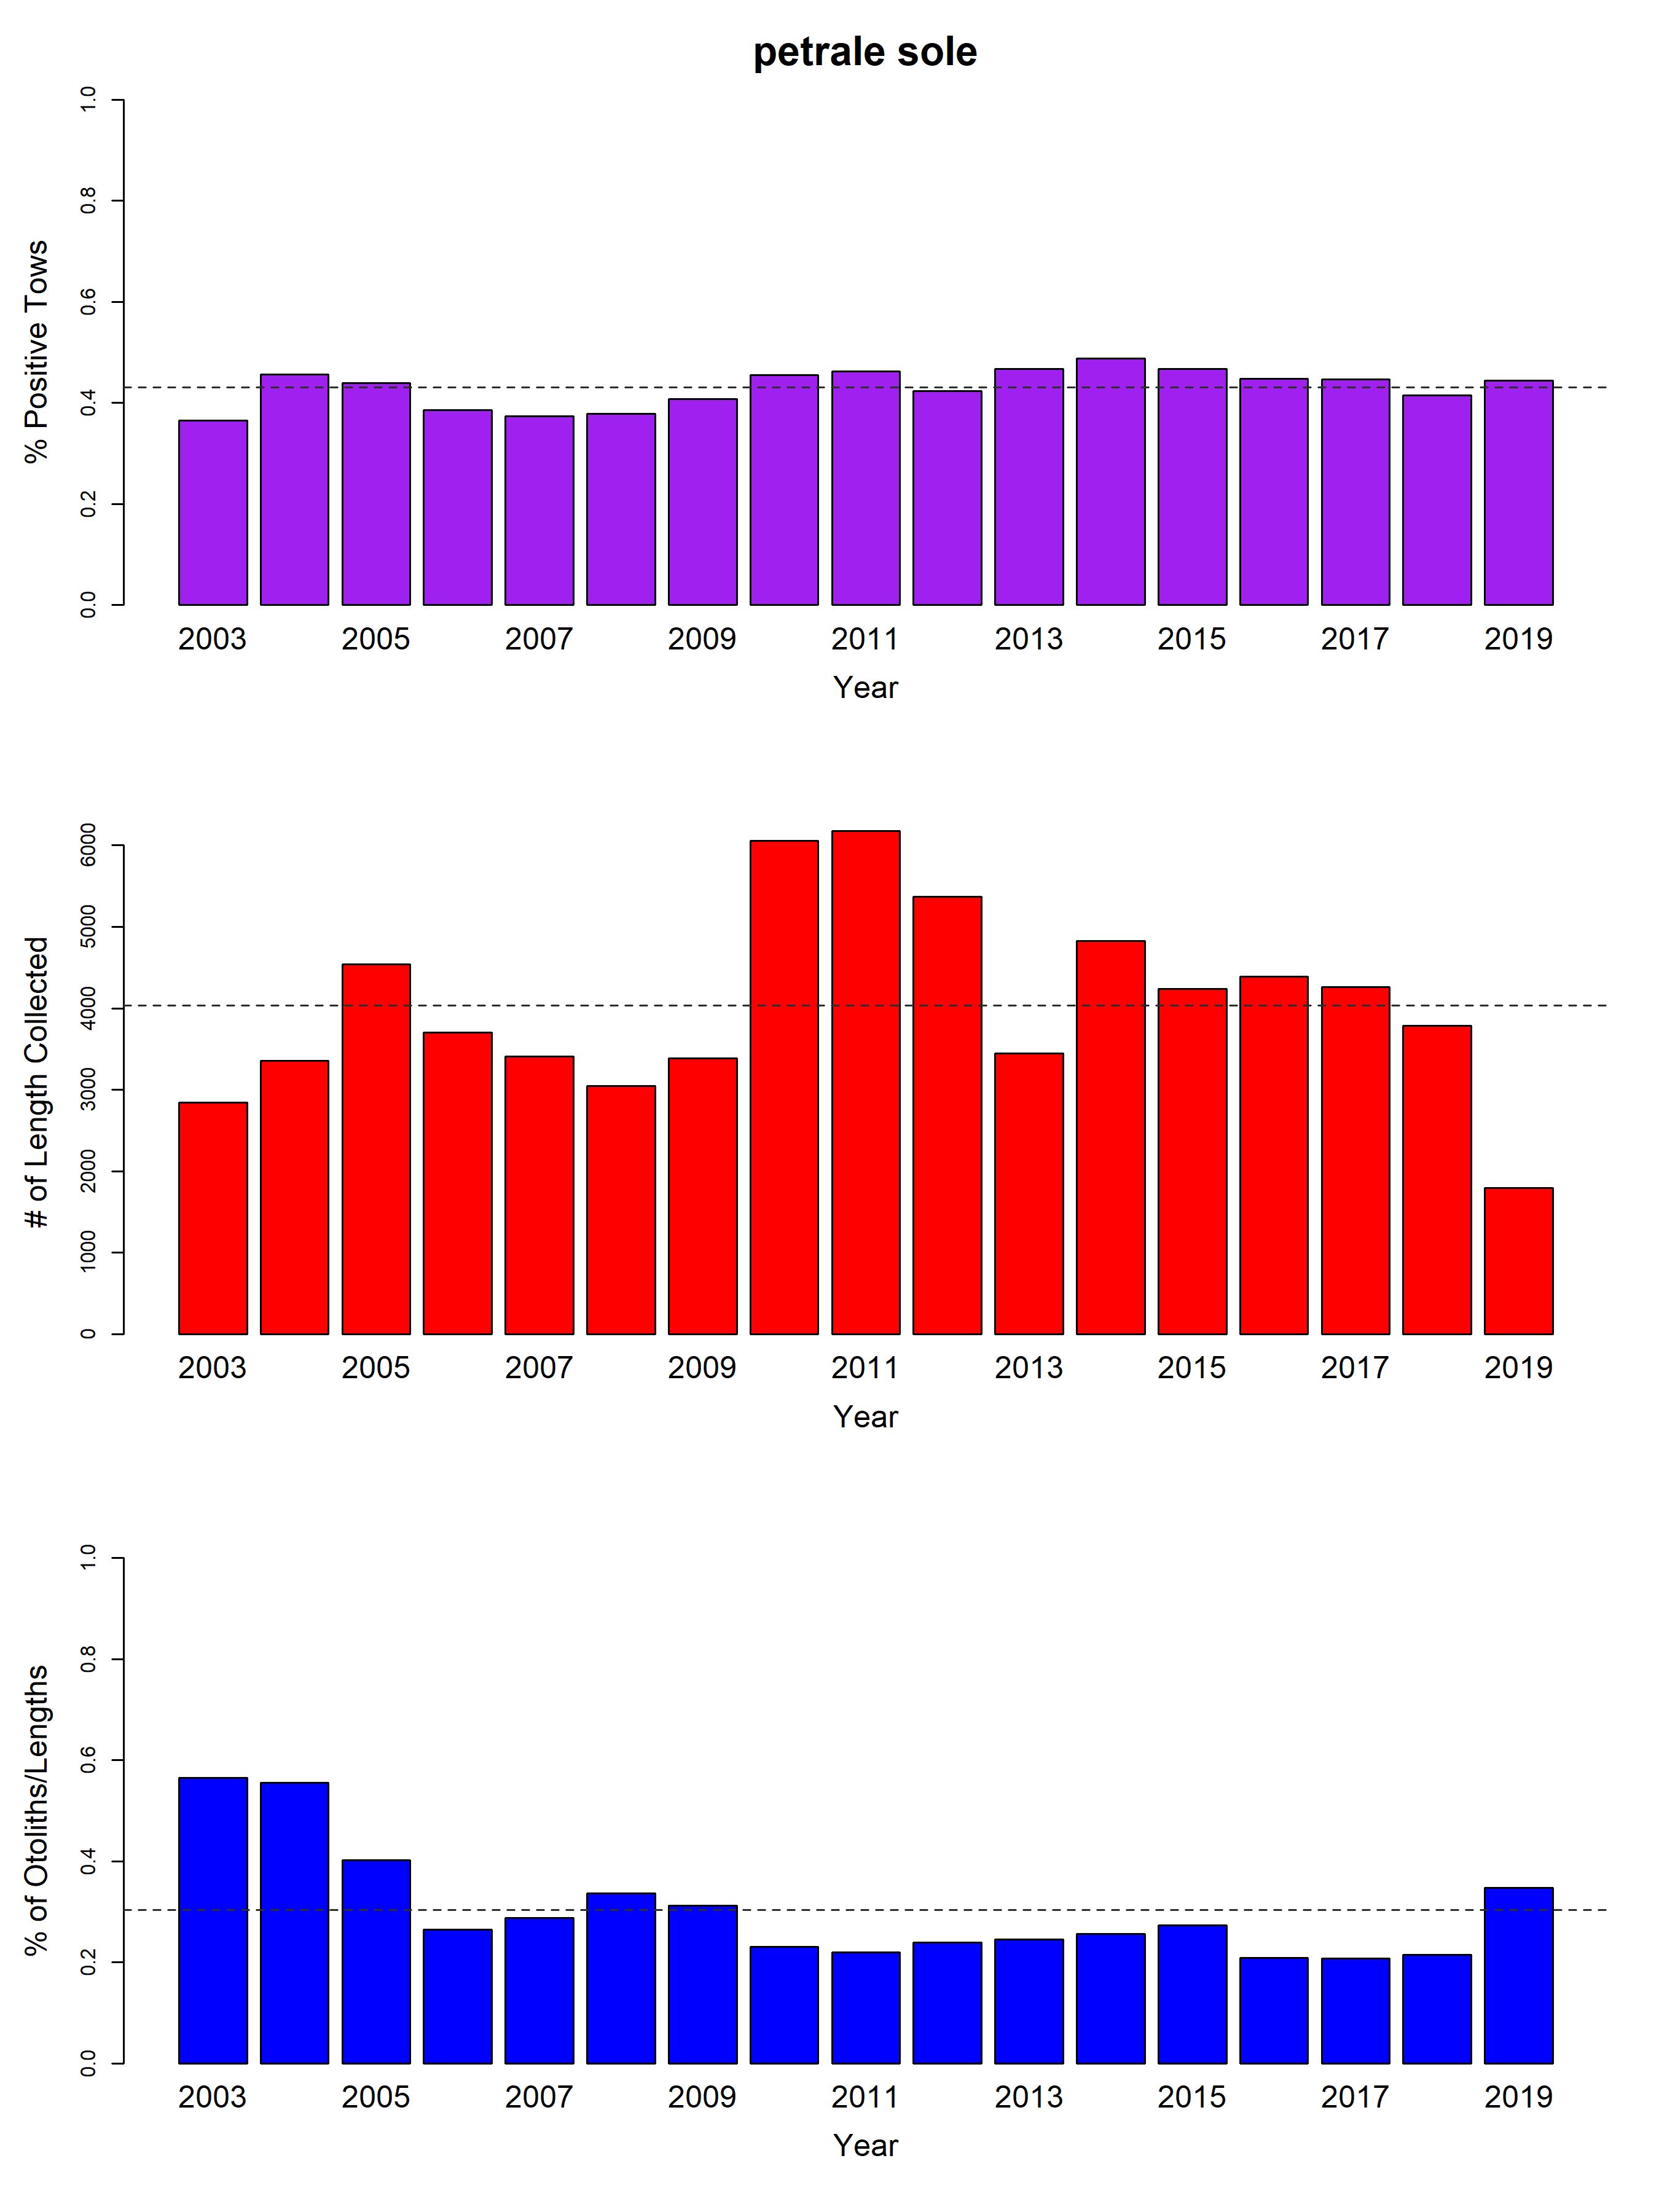
\includegraphics[width=0.6\textwidth,height=\textheight]{C:/Assessments/2020/survey_summary/sum_plots/petrale_sole_survey_stats.png}
\FloatBarrier  

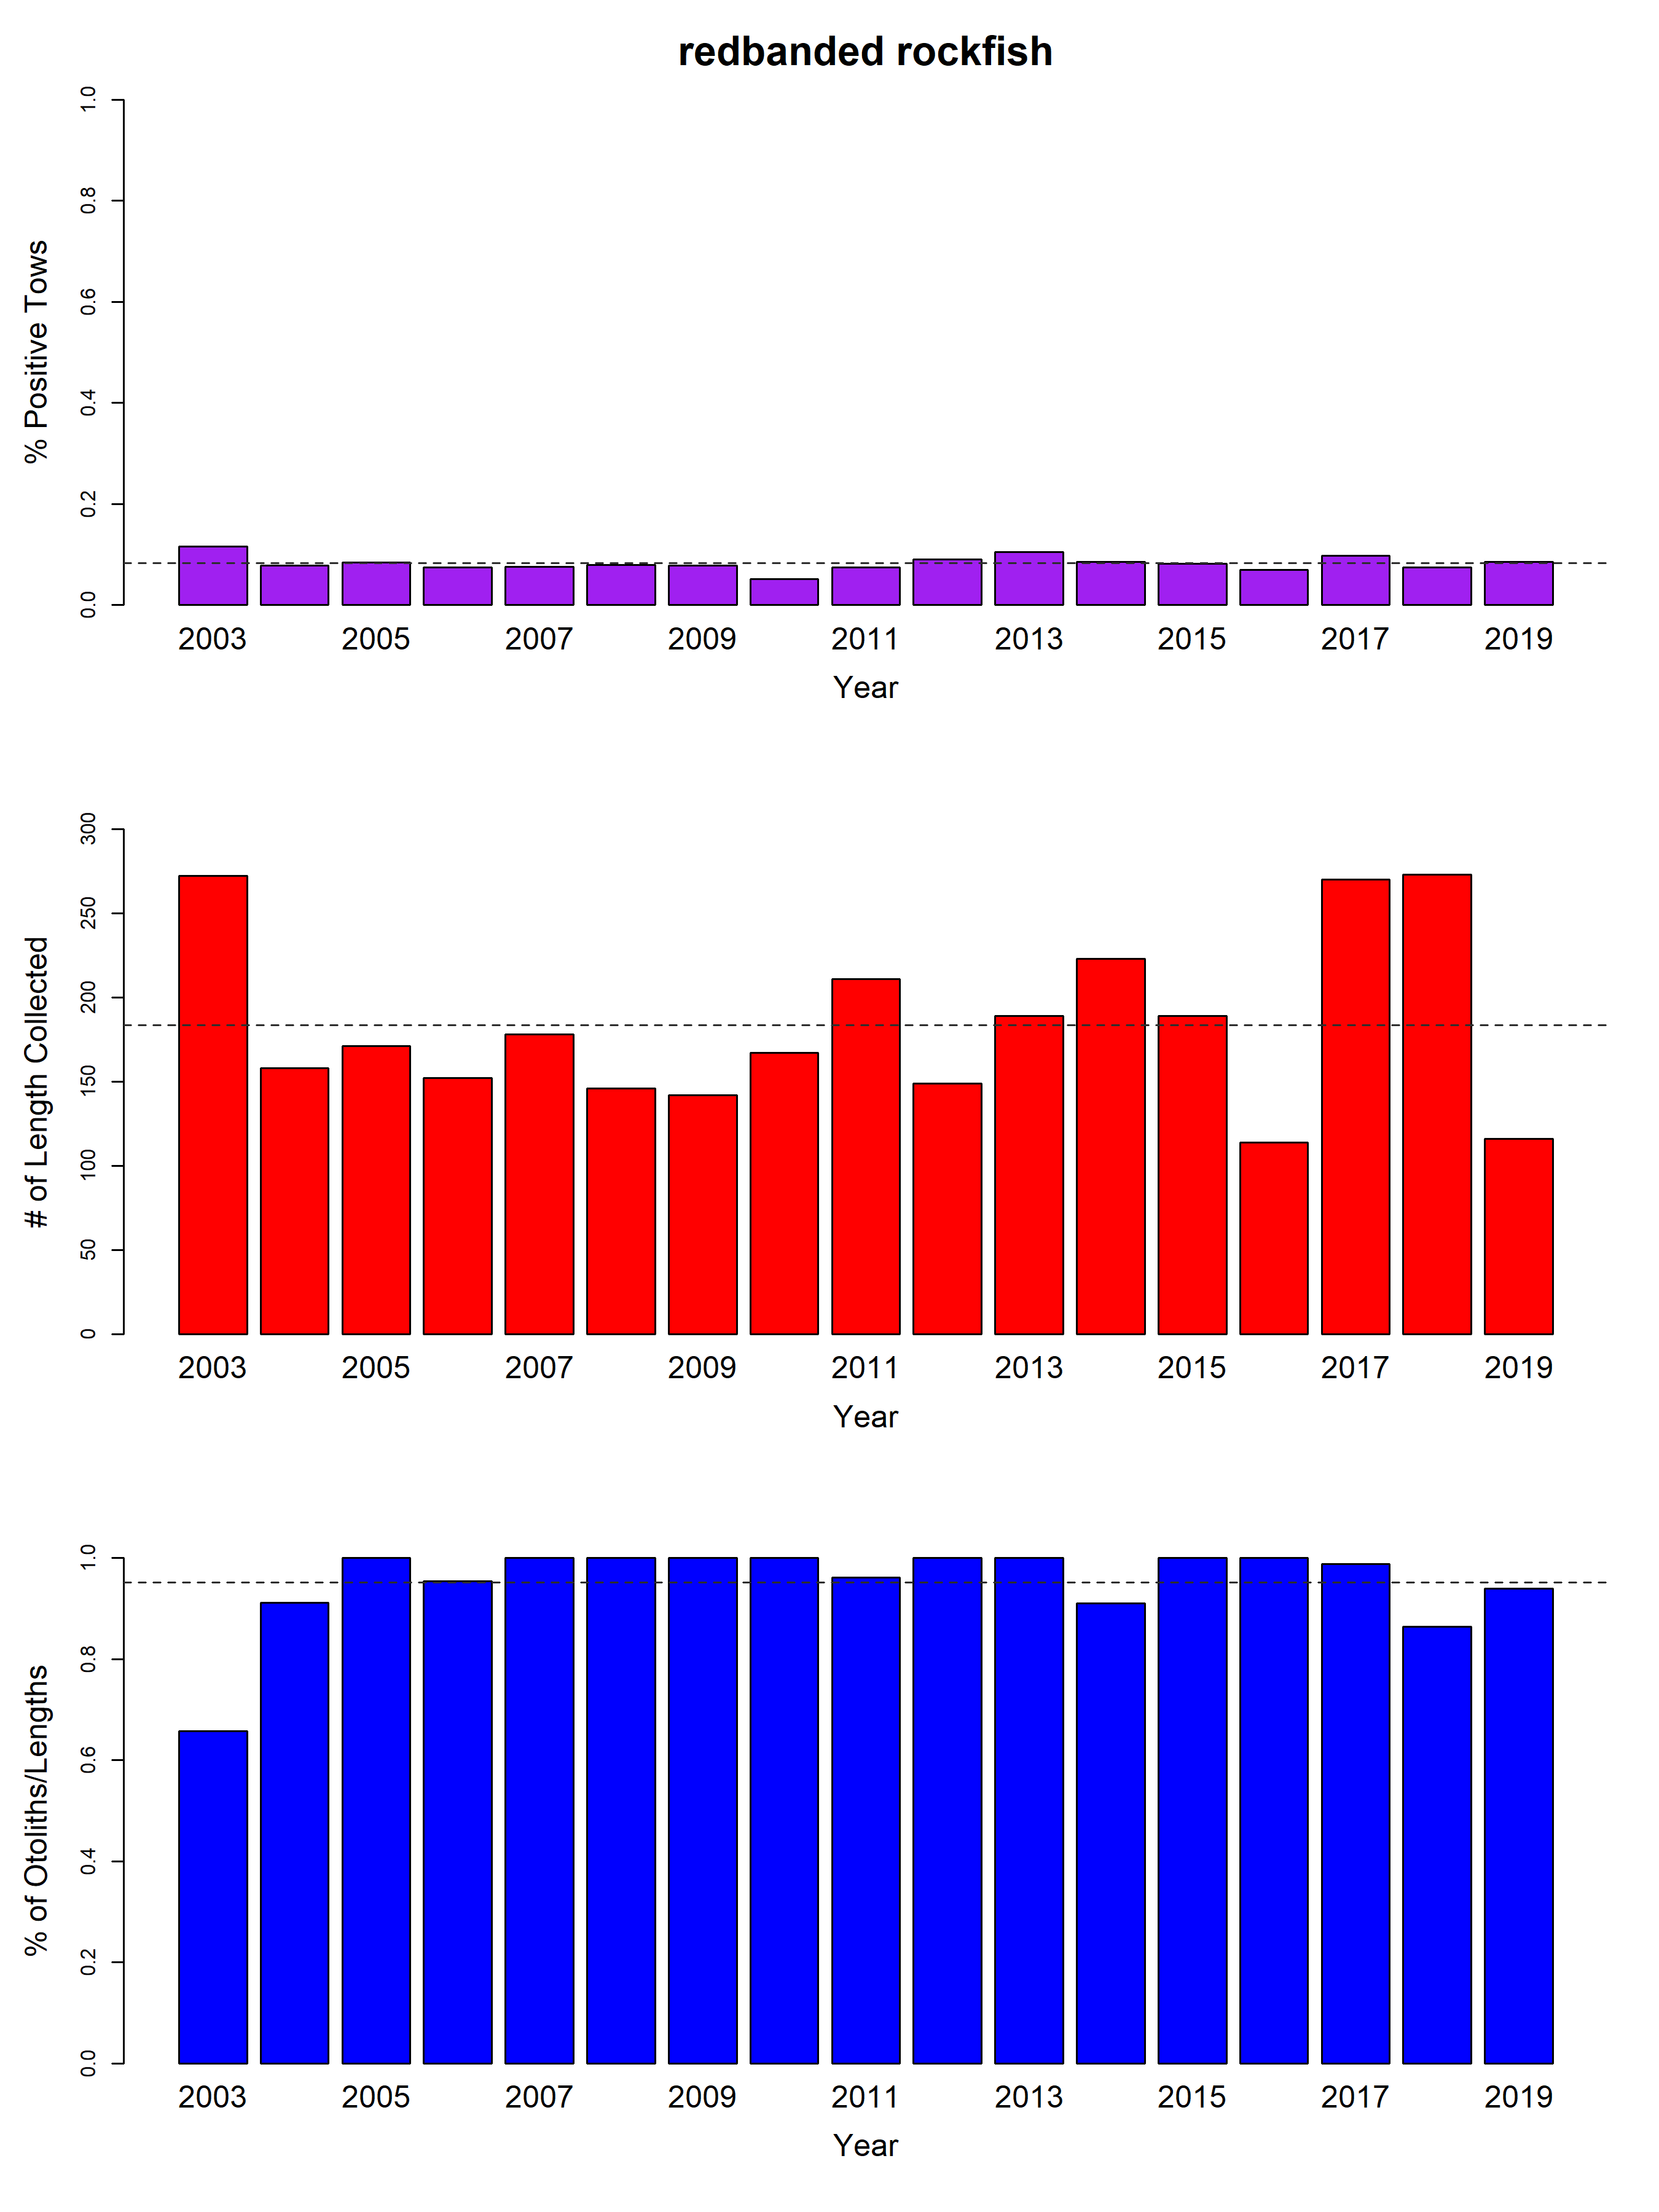
\includegraphics[width=0.6\textwidth,height=\textheight]{C:/Assessments/2020/survey_summary/sum_plots/redbanded_rockfish_survey_stats.png}
\FloatBarrier  

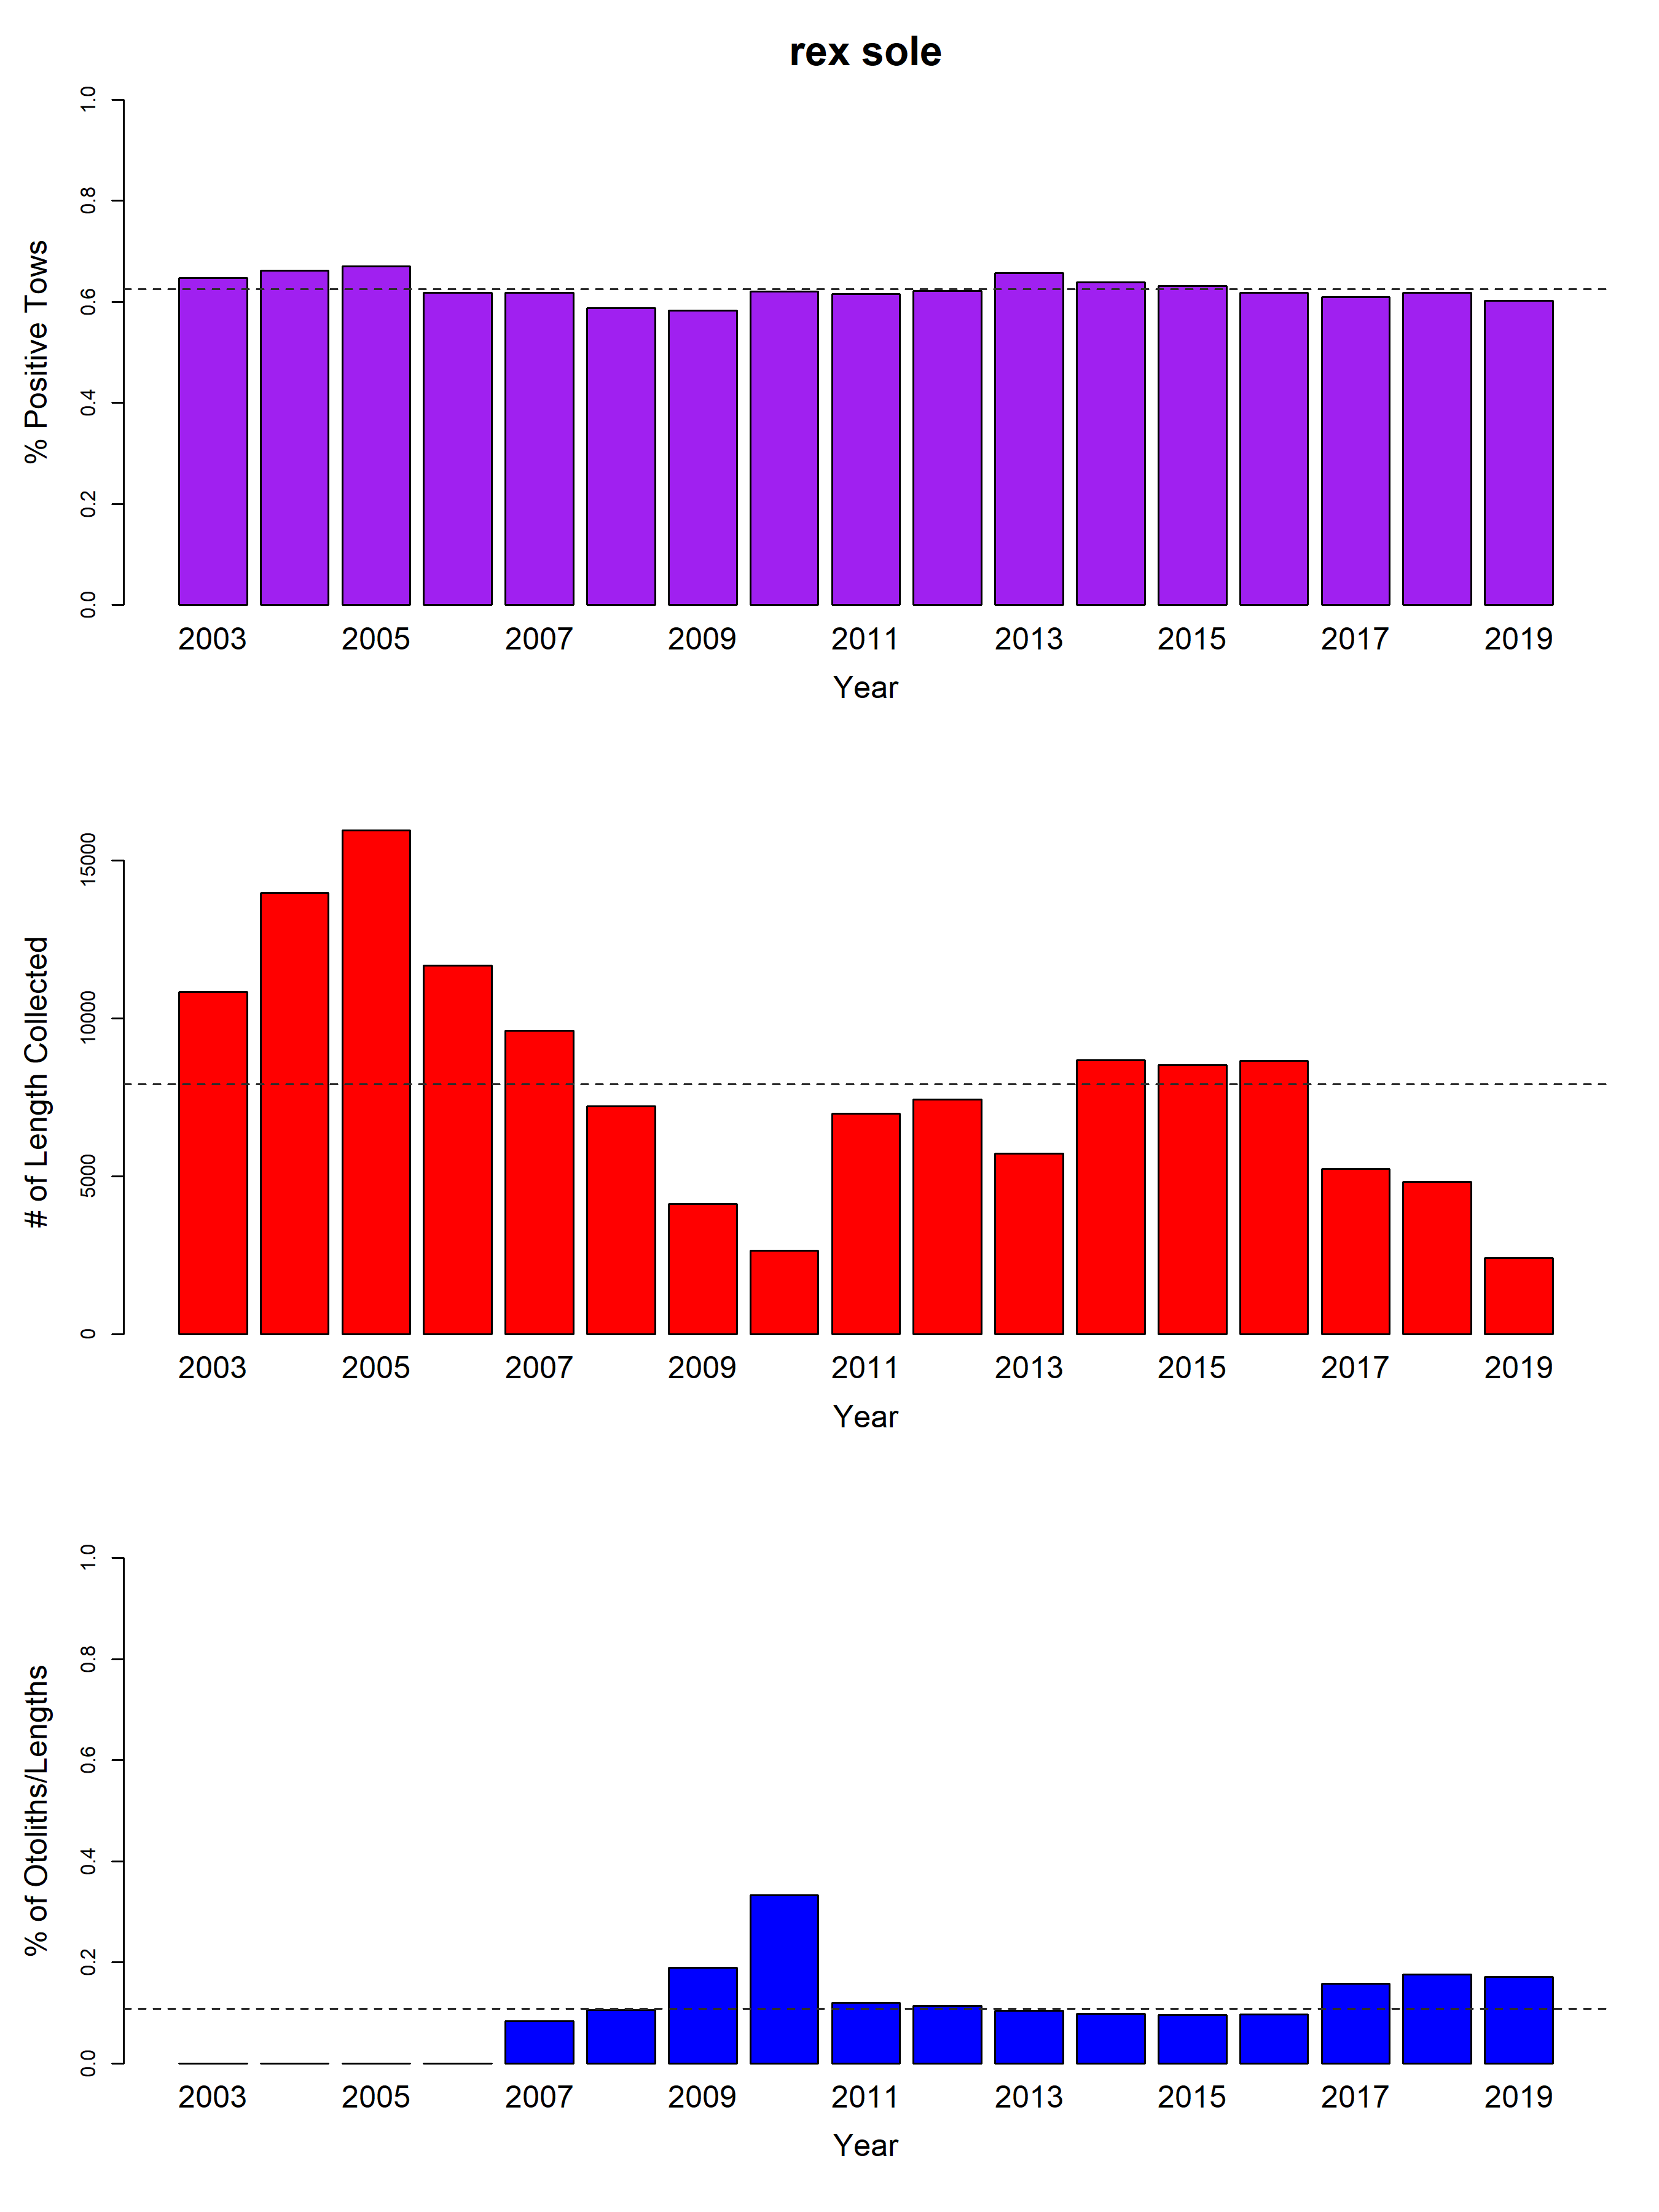
\includegraphics[width=0.6\textwidth,height=\textheight]{C:/Assessments/2020/survey_summary/sum_plots/rex_sole_survey_stats.png}
\FloatBarrier  

\FloatBarrier

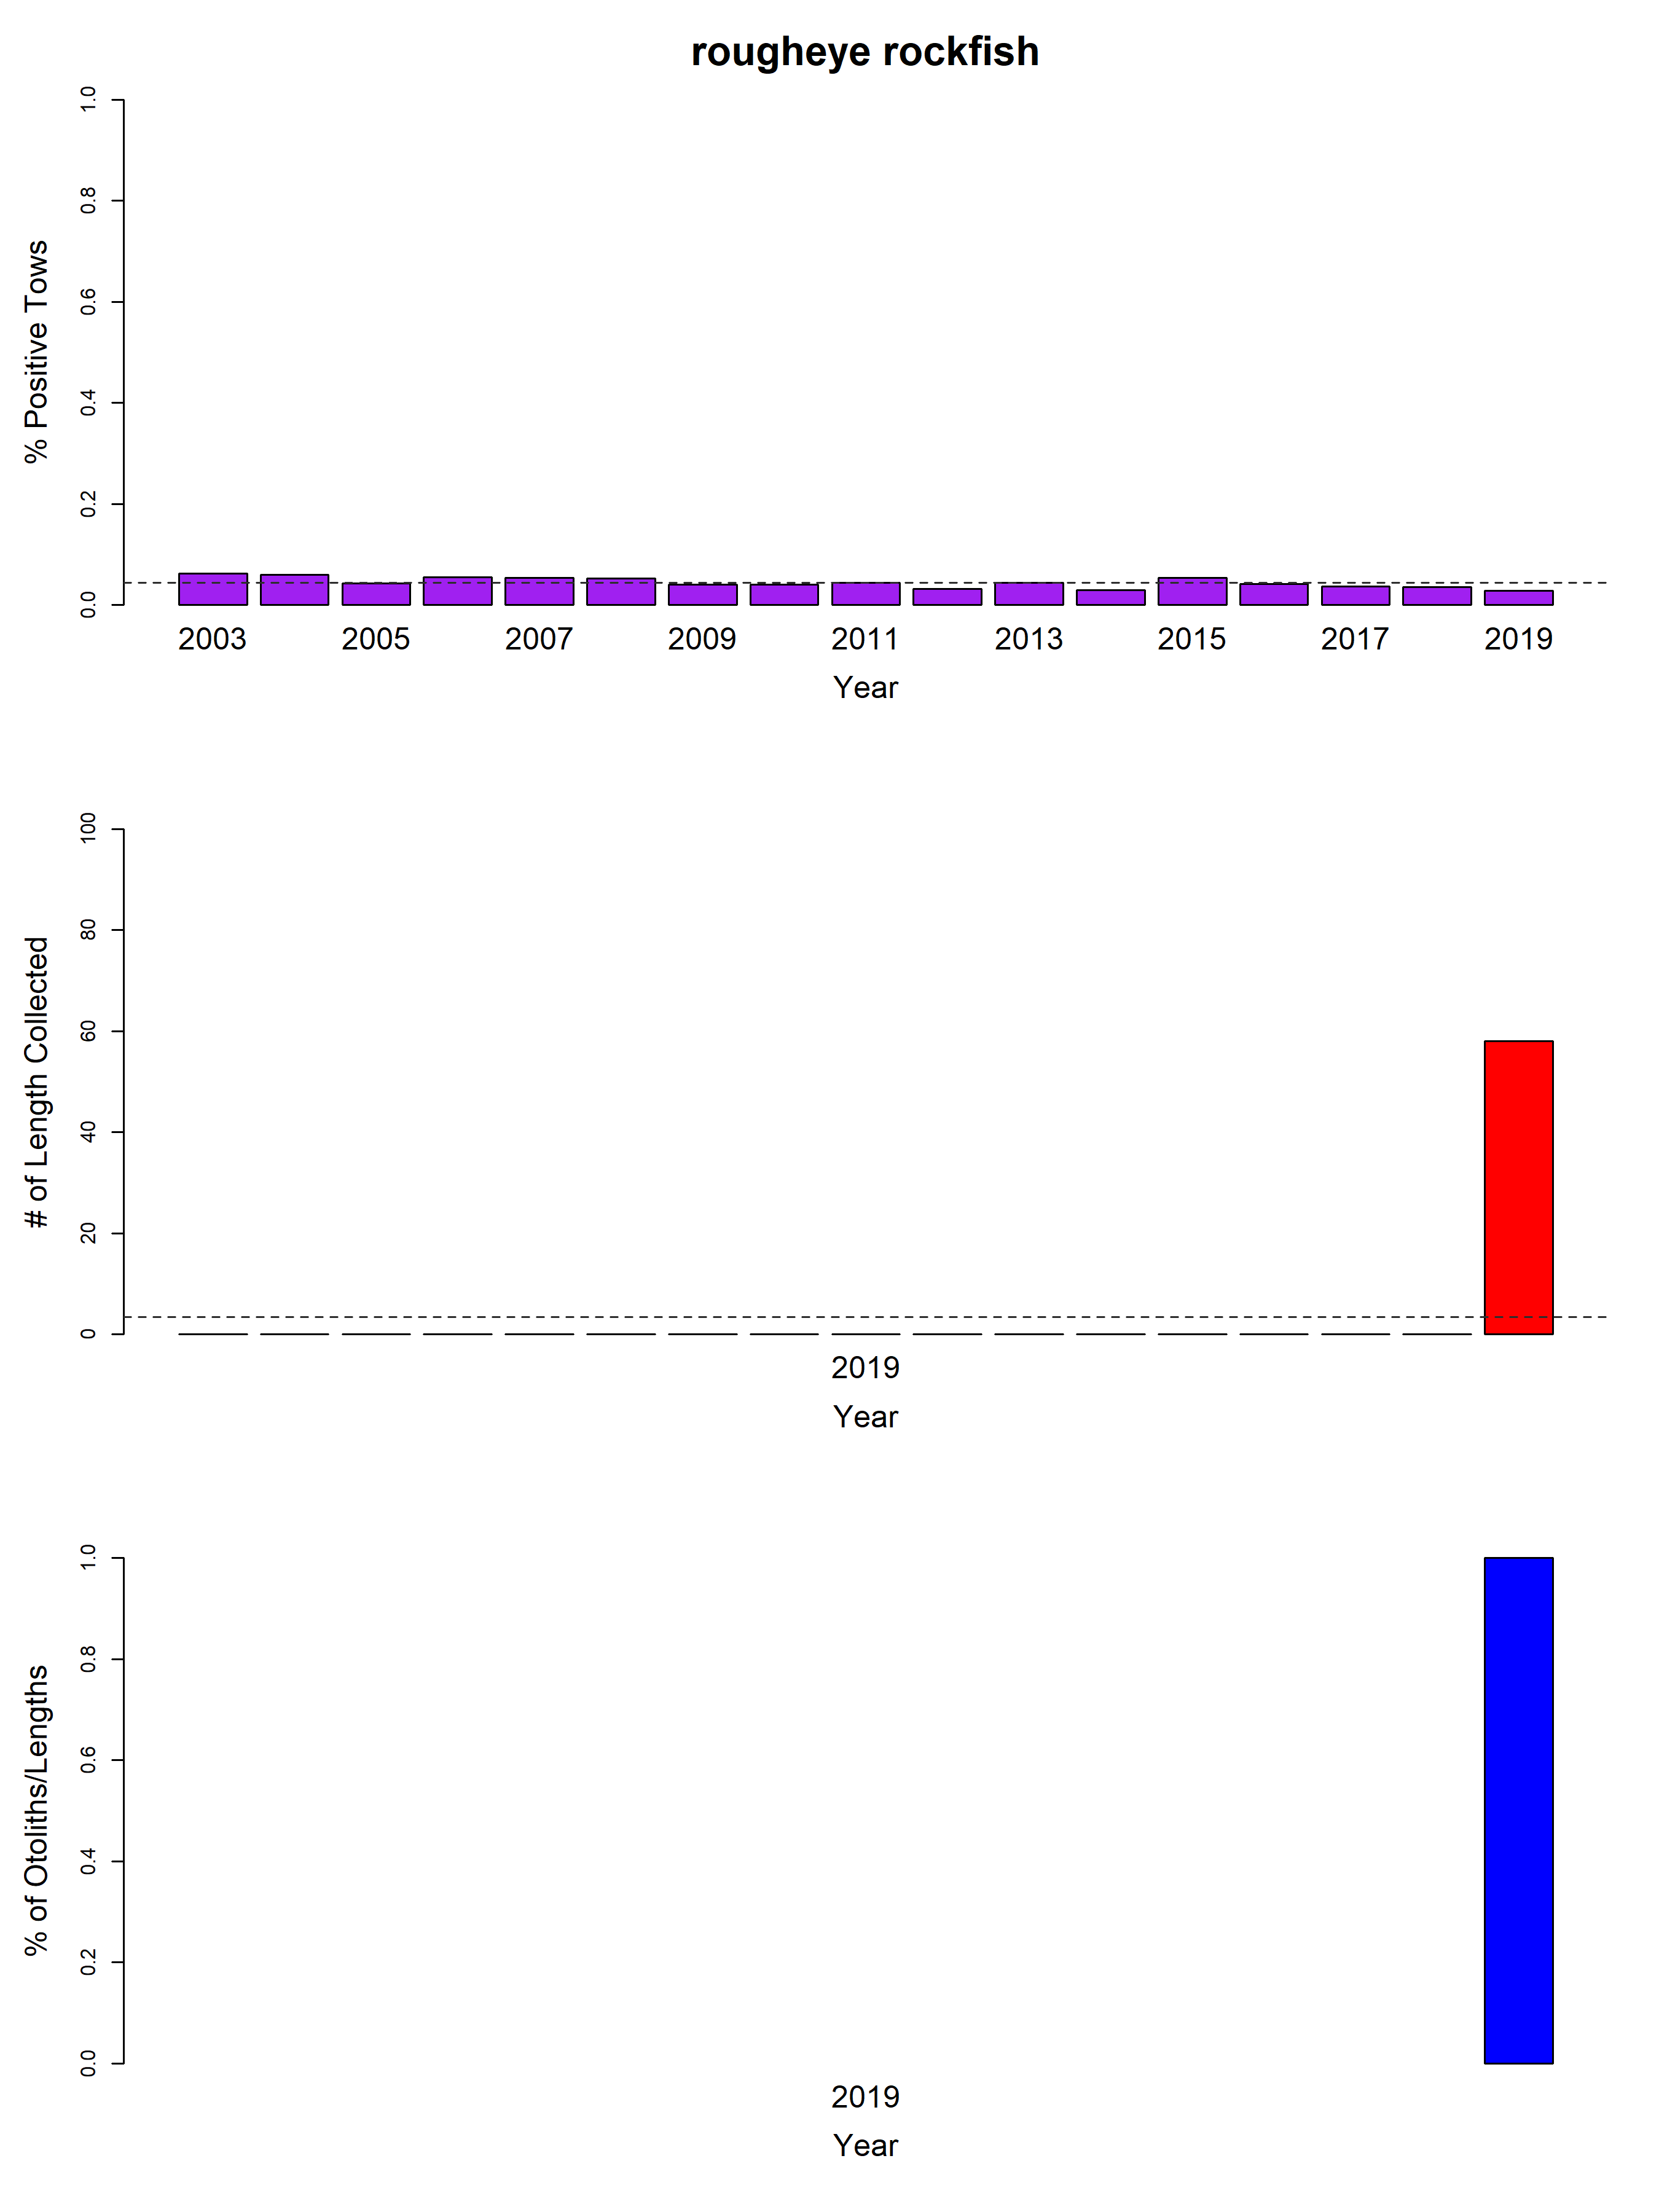
\includegraphics[width=0.6\textwidth,height=\textheight]{C:/Assessments/2020/survey_summary/sum_plots/rougheye_rockfish_survey_stats.png}
\FloatBarrier  

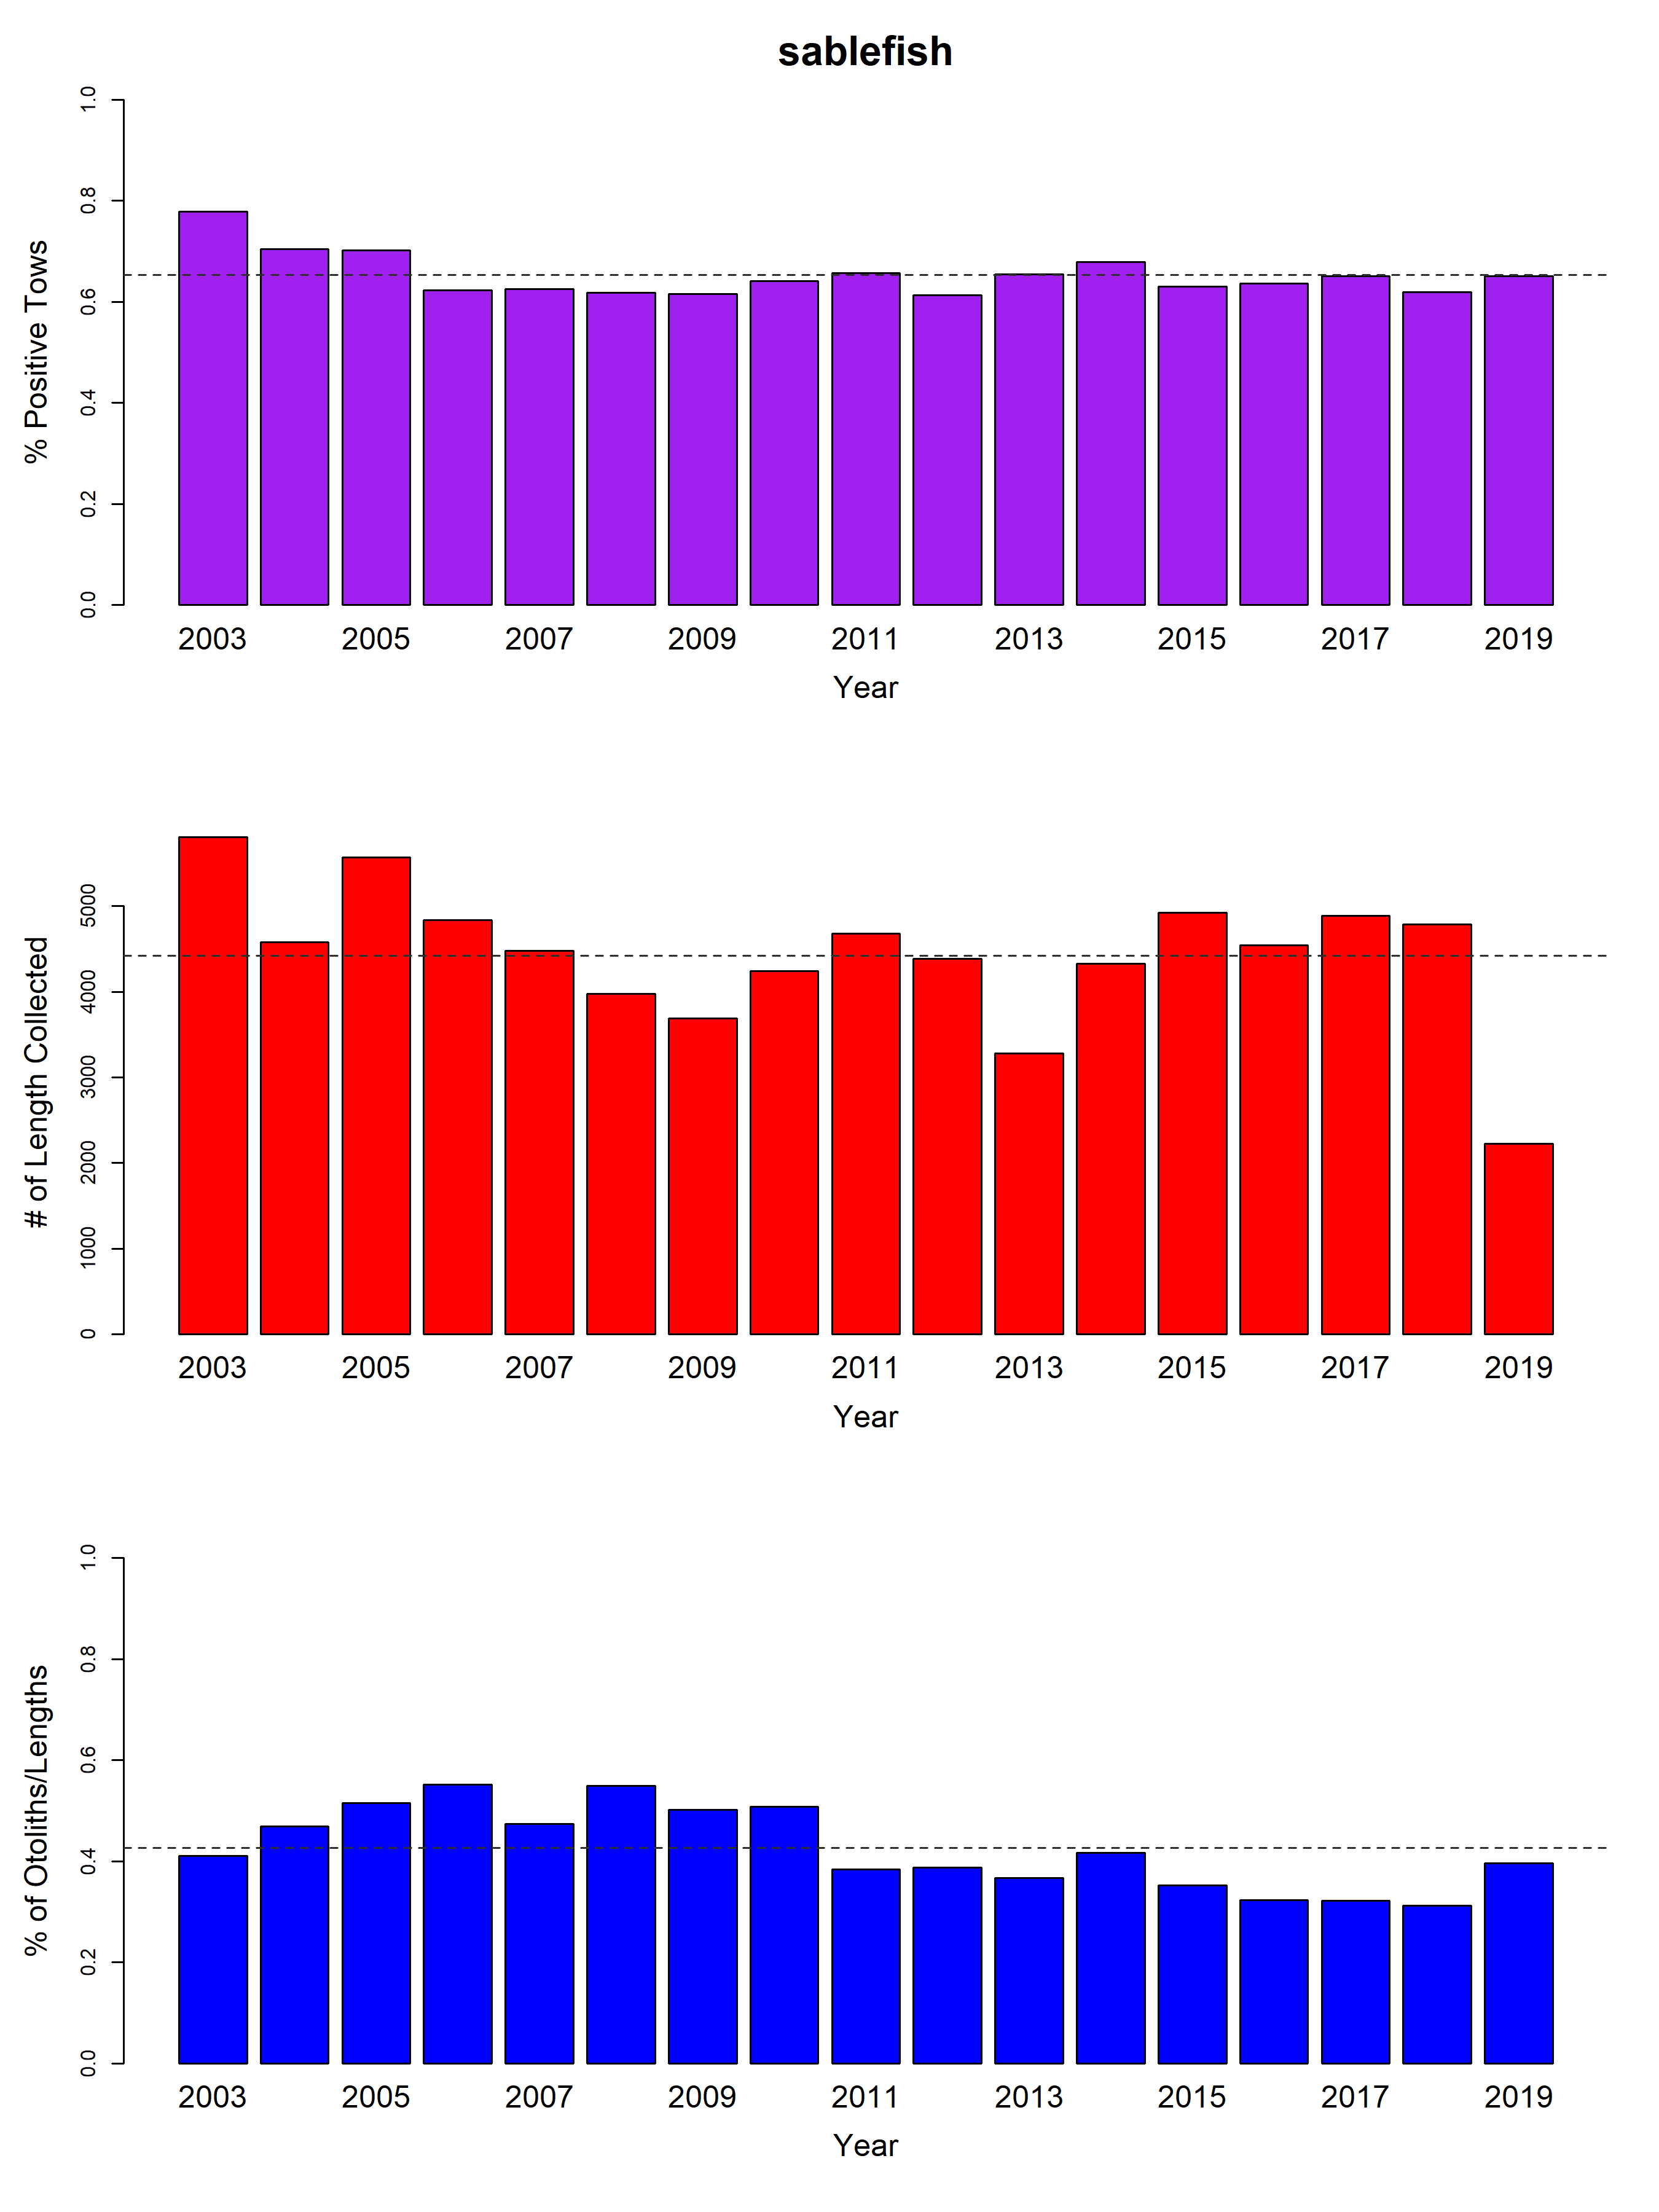
\includegraphics[width=0.6\textwidth,height=\textheight]{C:/Assessments/2020/survey_summary/sum_plots/sablefish_survey_stats.png}
\FloatBarrier  

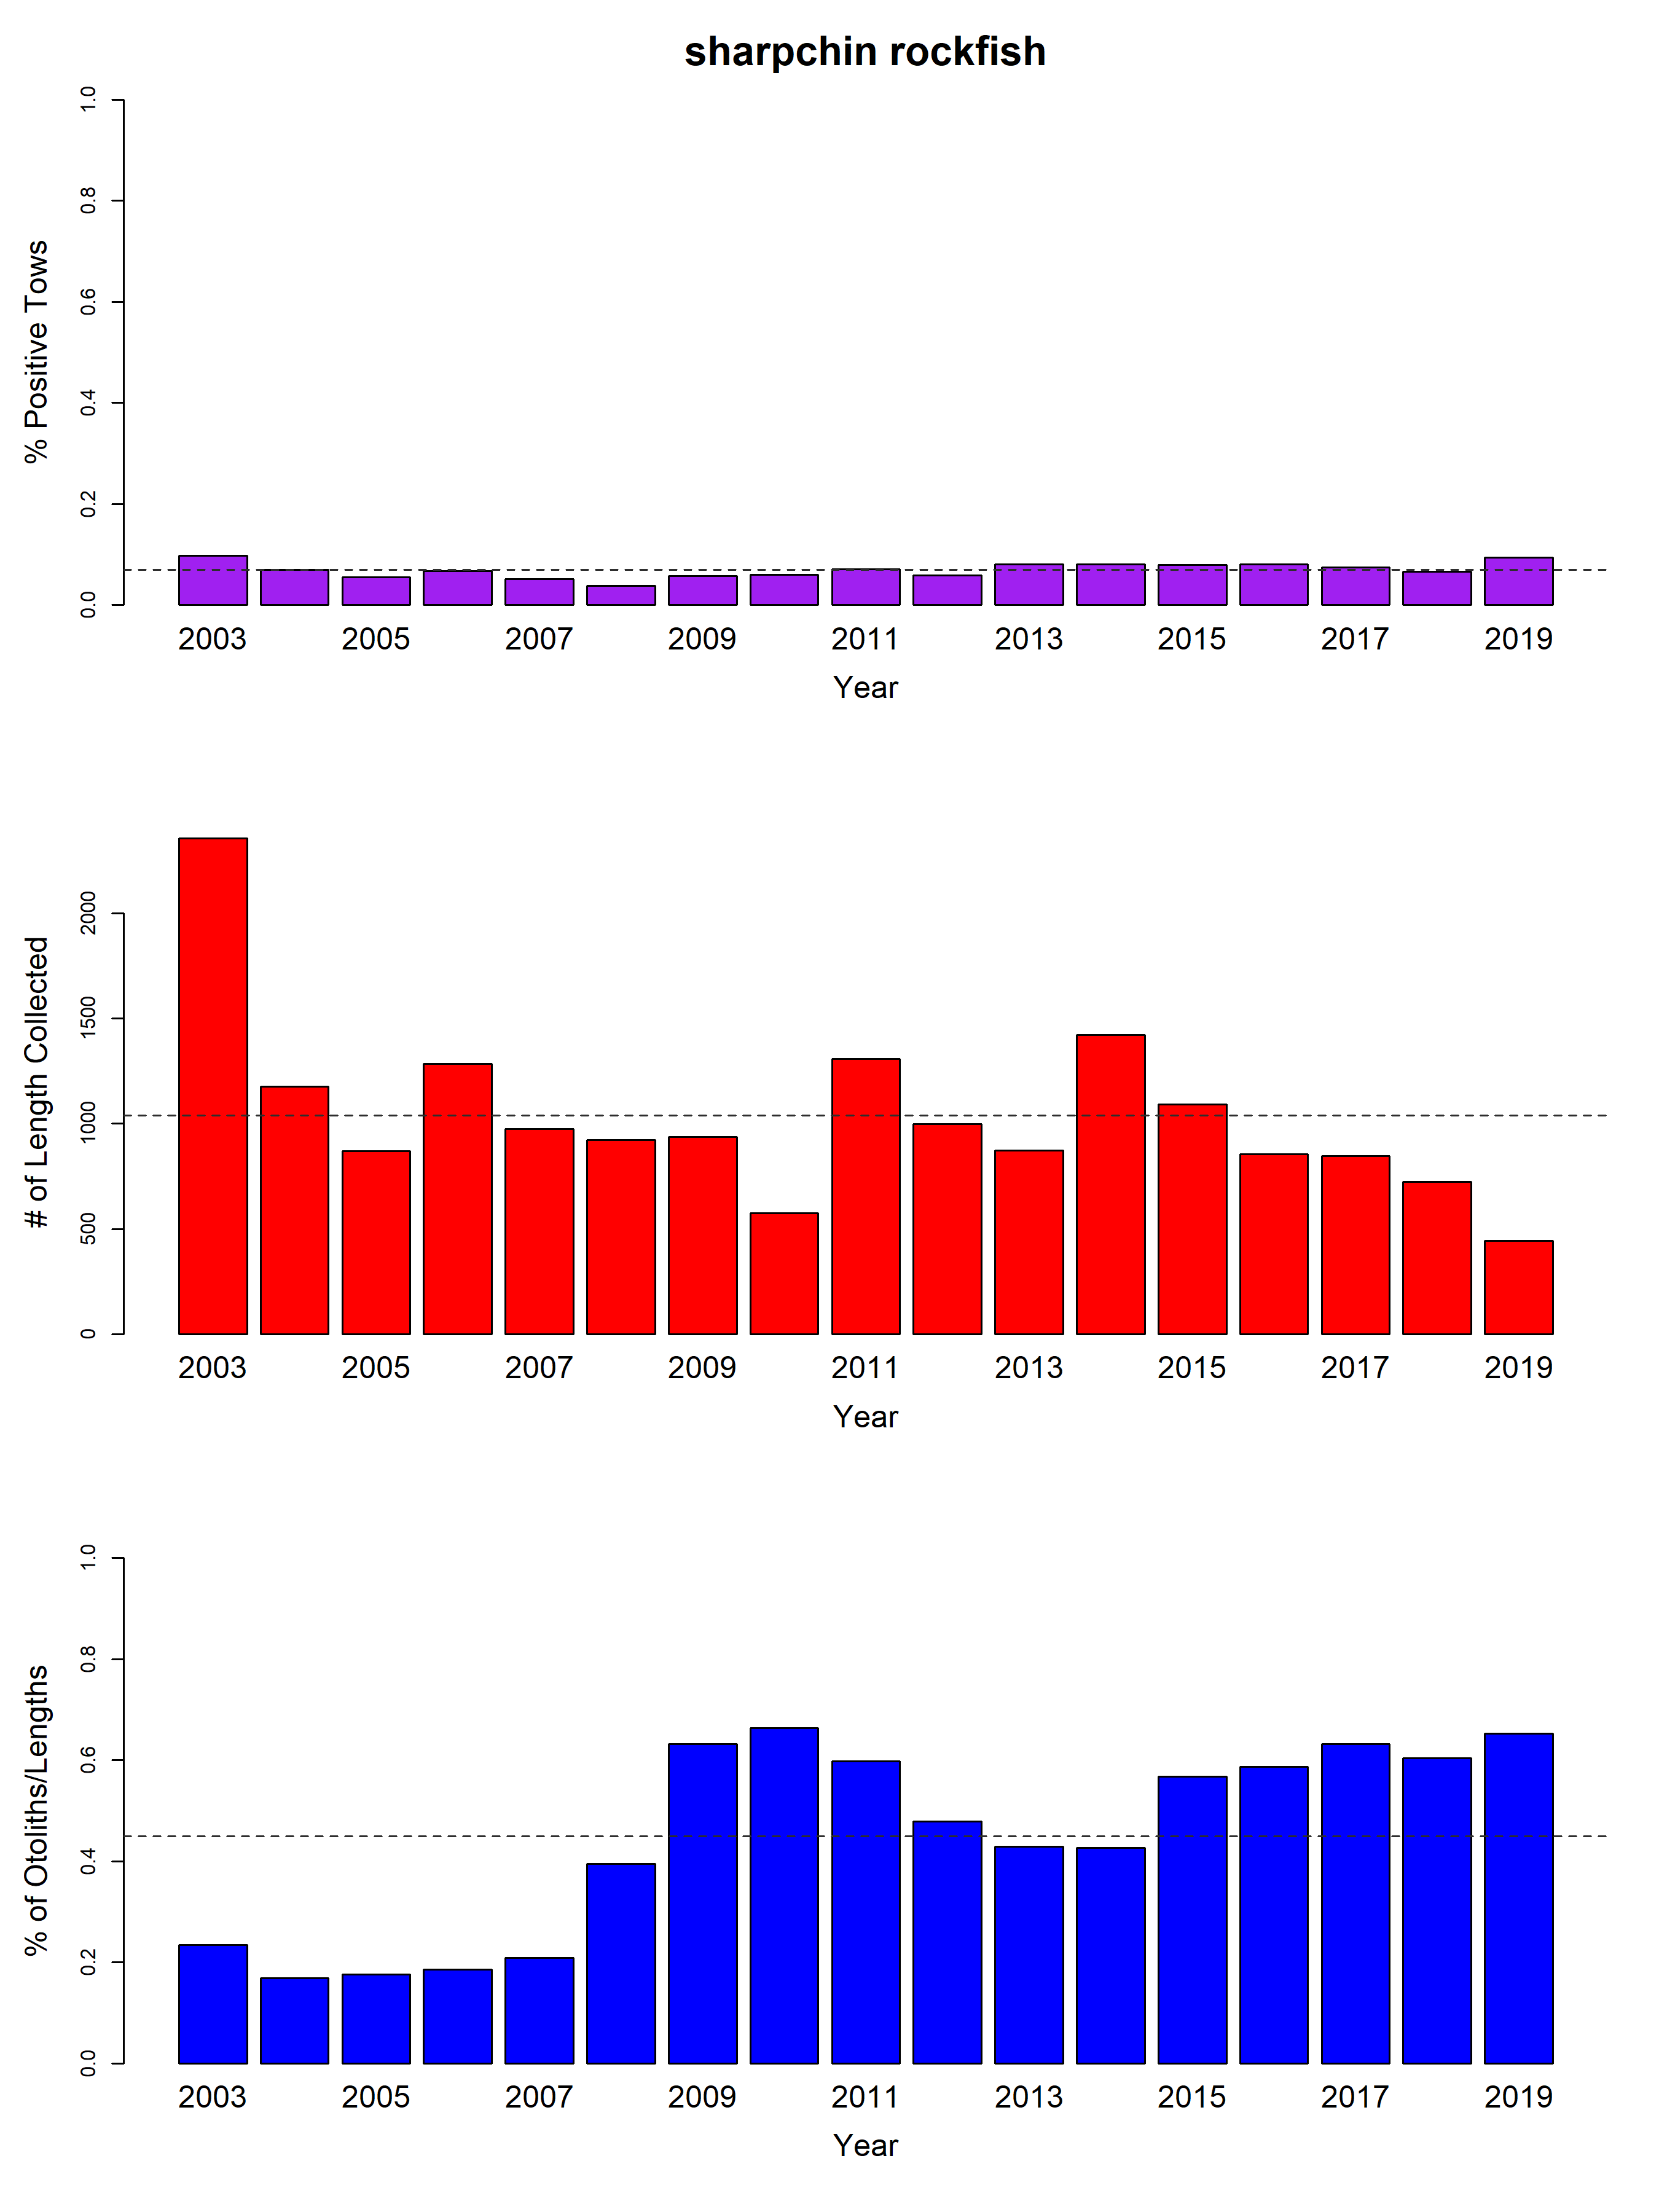
\includegraphics[width=0.6\textwidth,height=\textheight]{C:/Assessments/2020/survey_summary/sum_plots/sharpchin_rockfish_survey_stats.png}
\FloatBarrier  

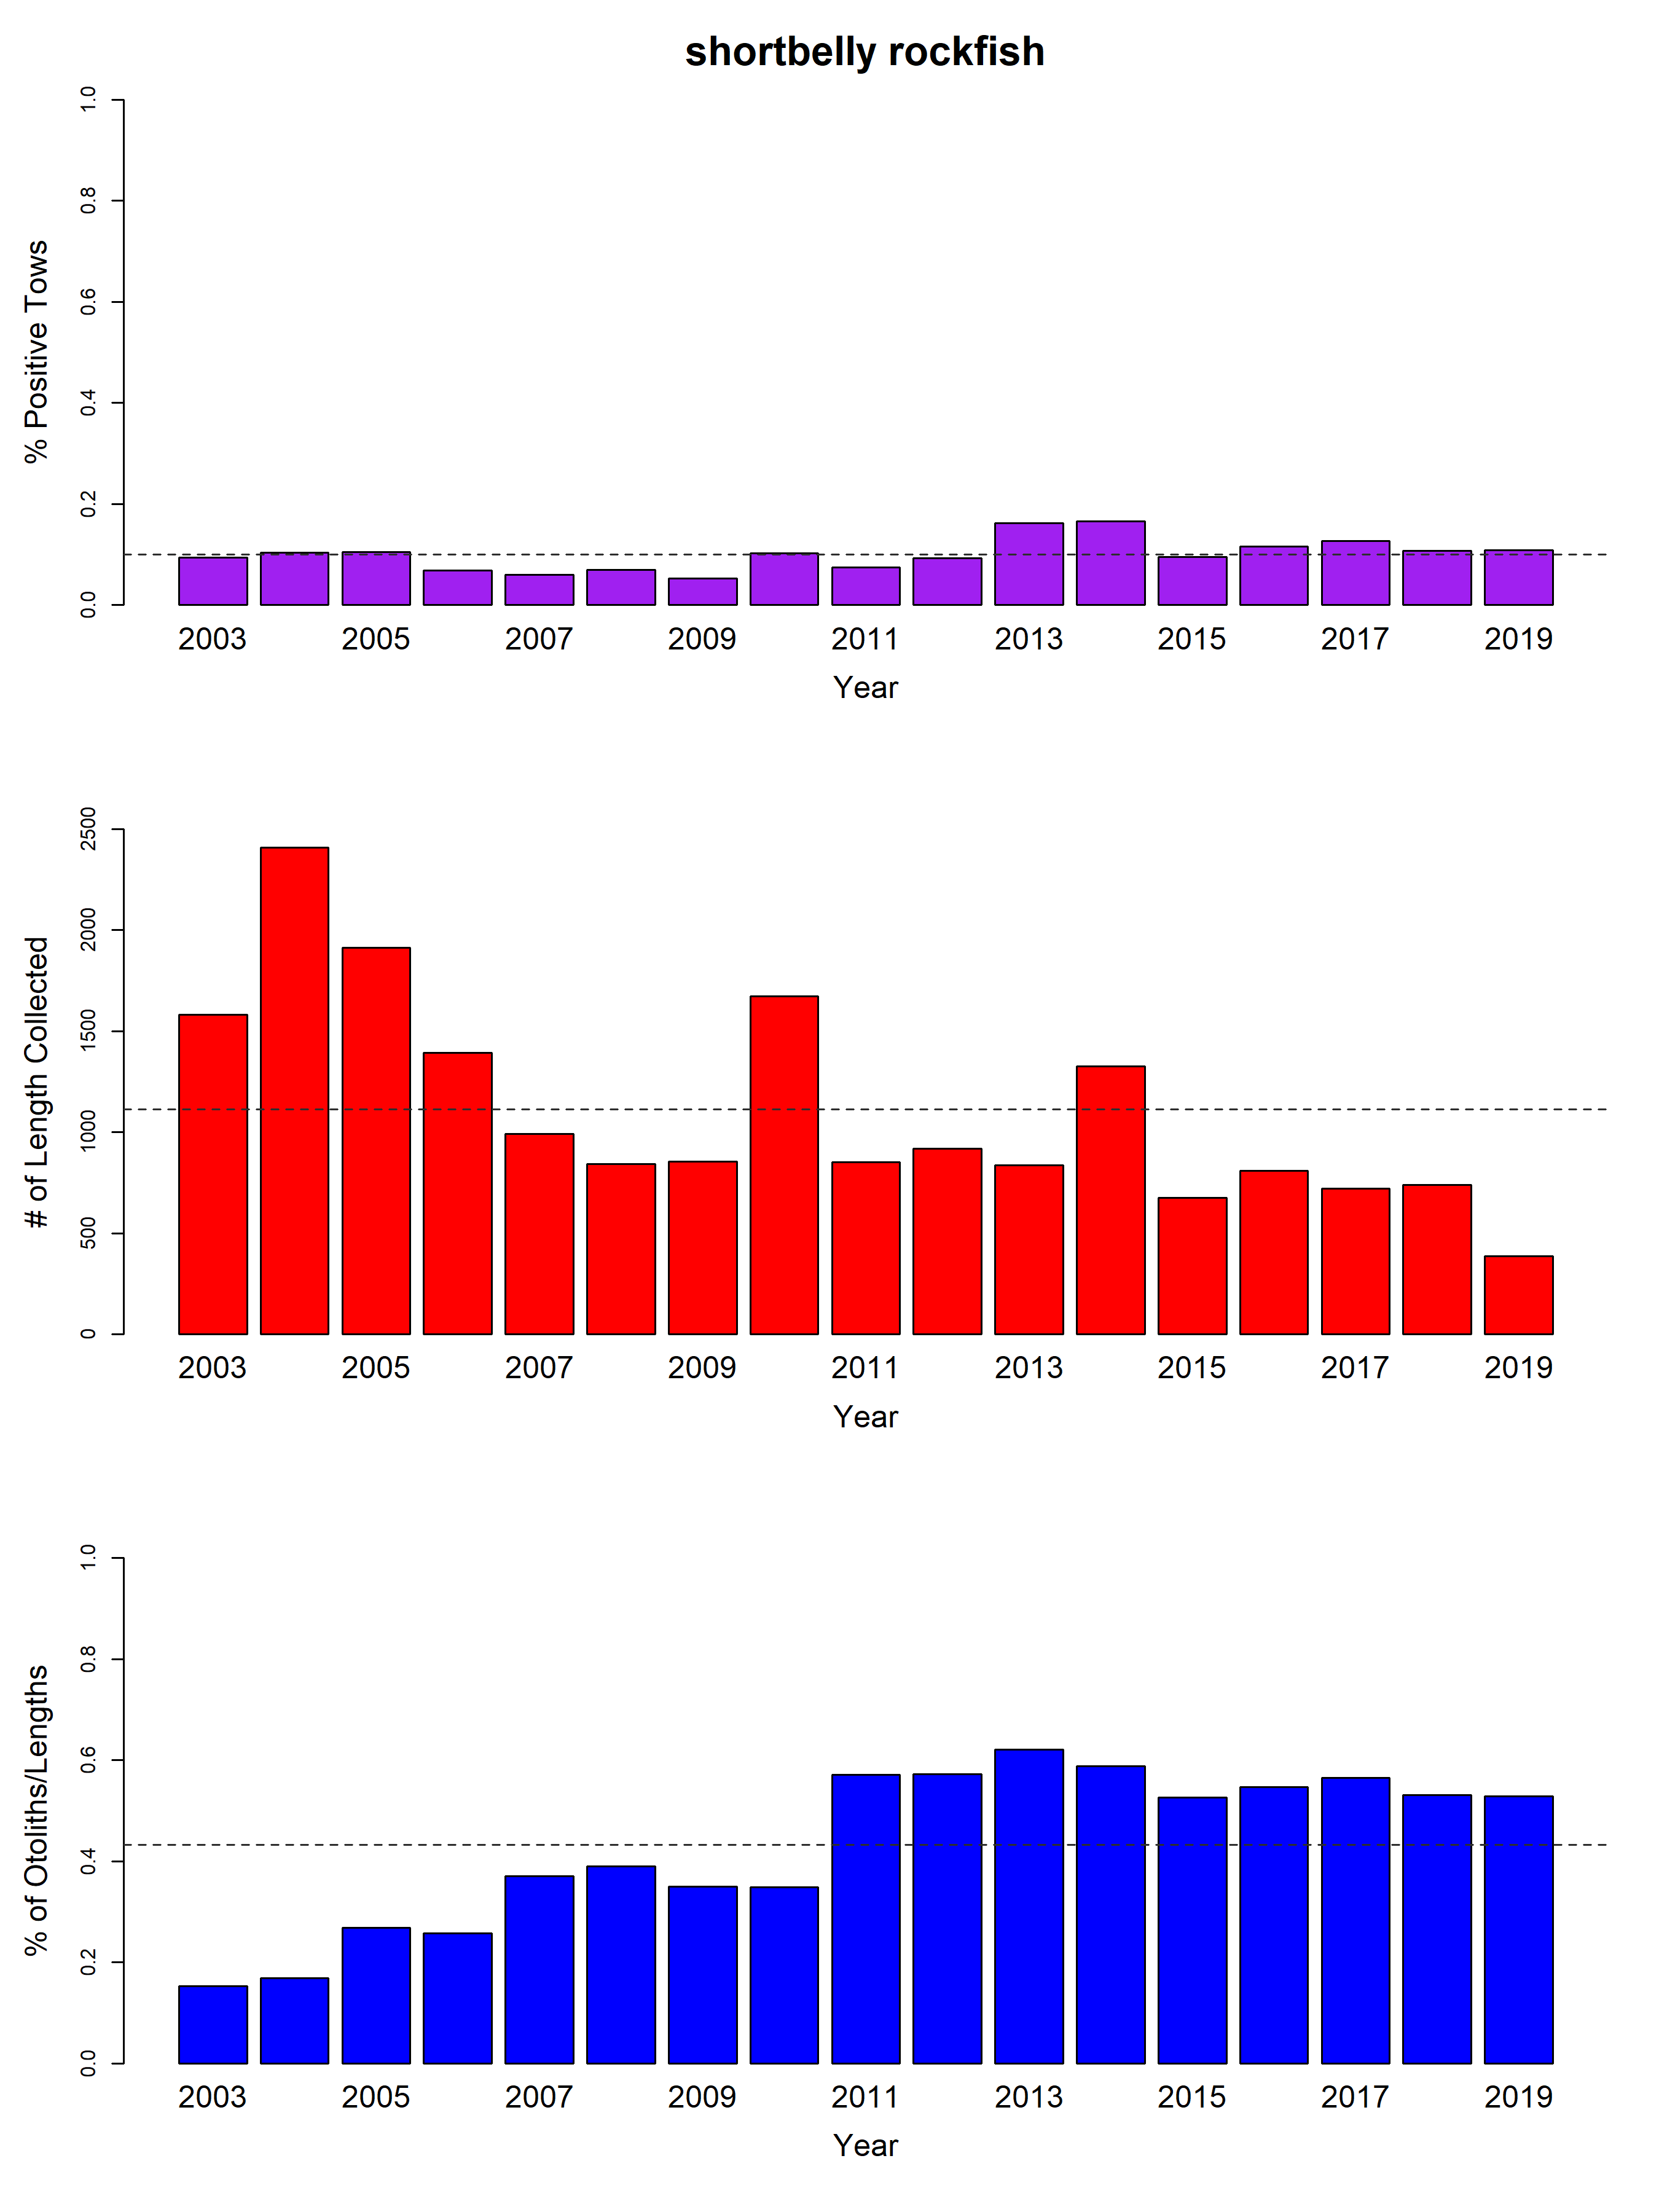
\includegraphics[width=0.6\textwidth,height=\textheight]{C:/Assessments/2020/survey_summary/sum_plots/shortbelly_rockfish_survey_stats.png}
\FloatBarrier  

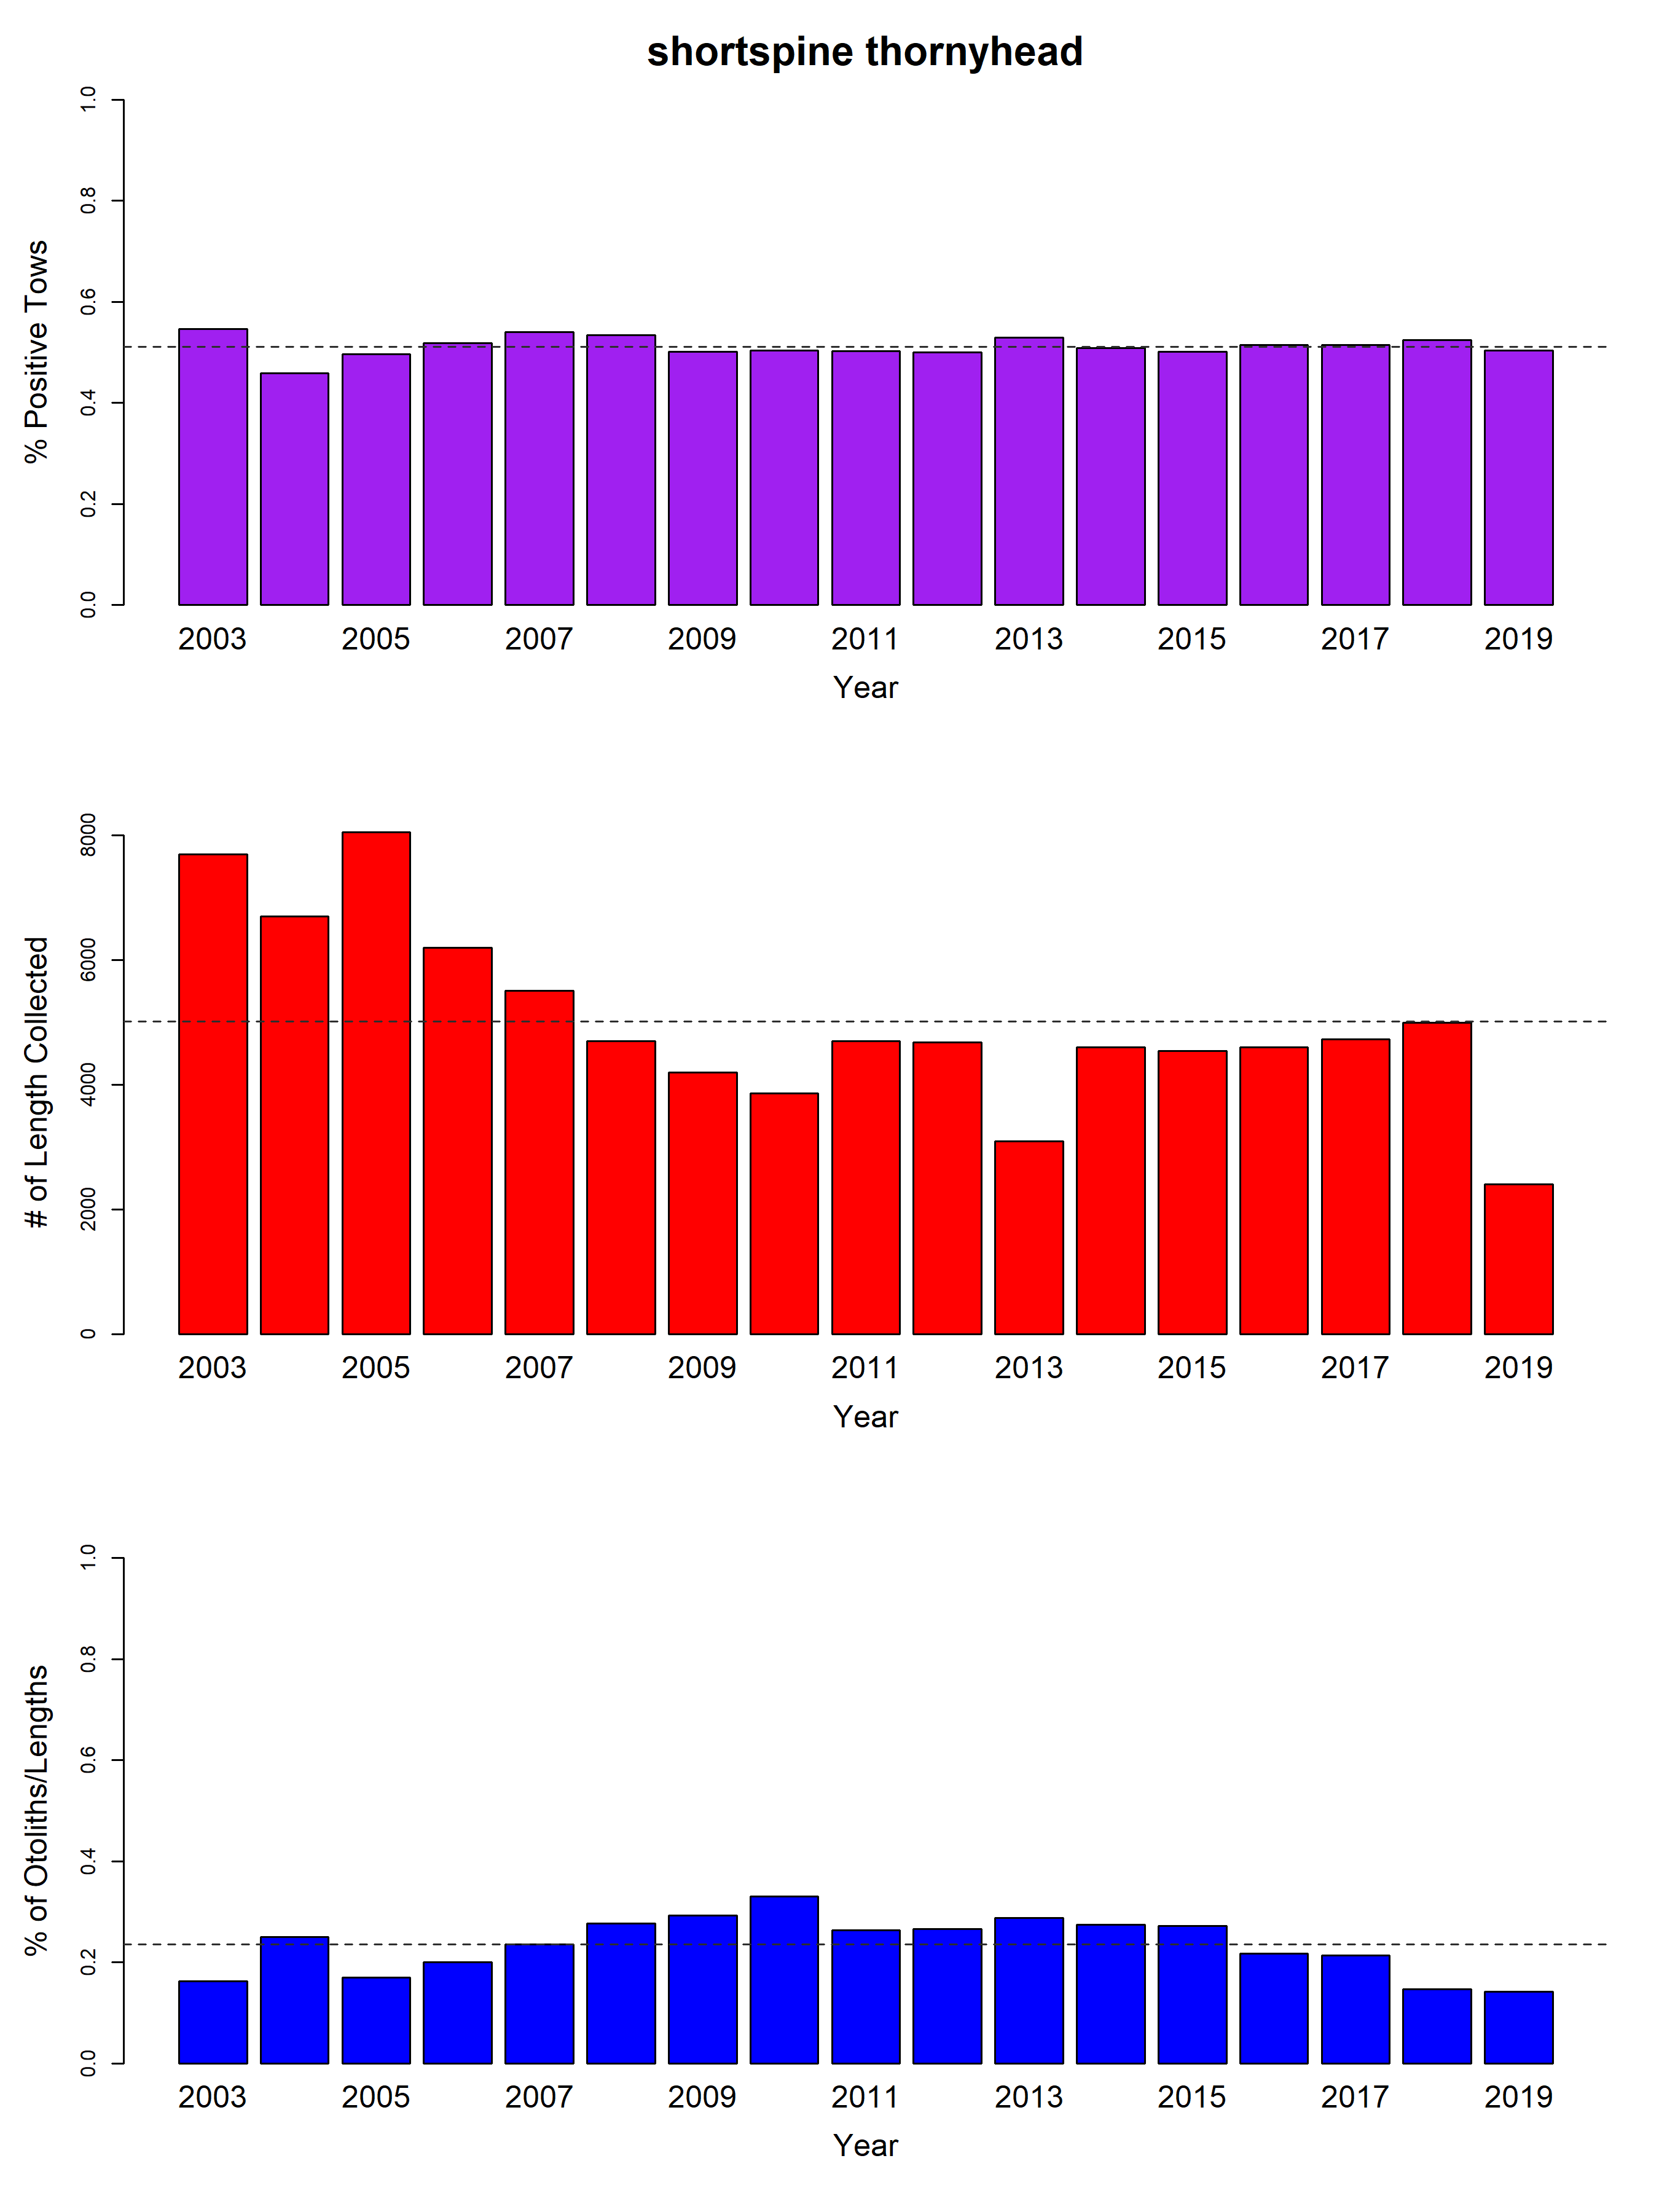
\includegraphics[width=0.6\textwidth,height=\textheight]{C:/Assessments/2020/survey_summary/sum_plots/shortspine_thornyhead_survey_stats.png}
\FloatBarrier  

\FloatBarrier

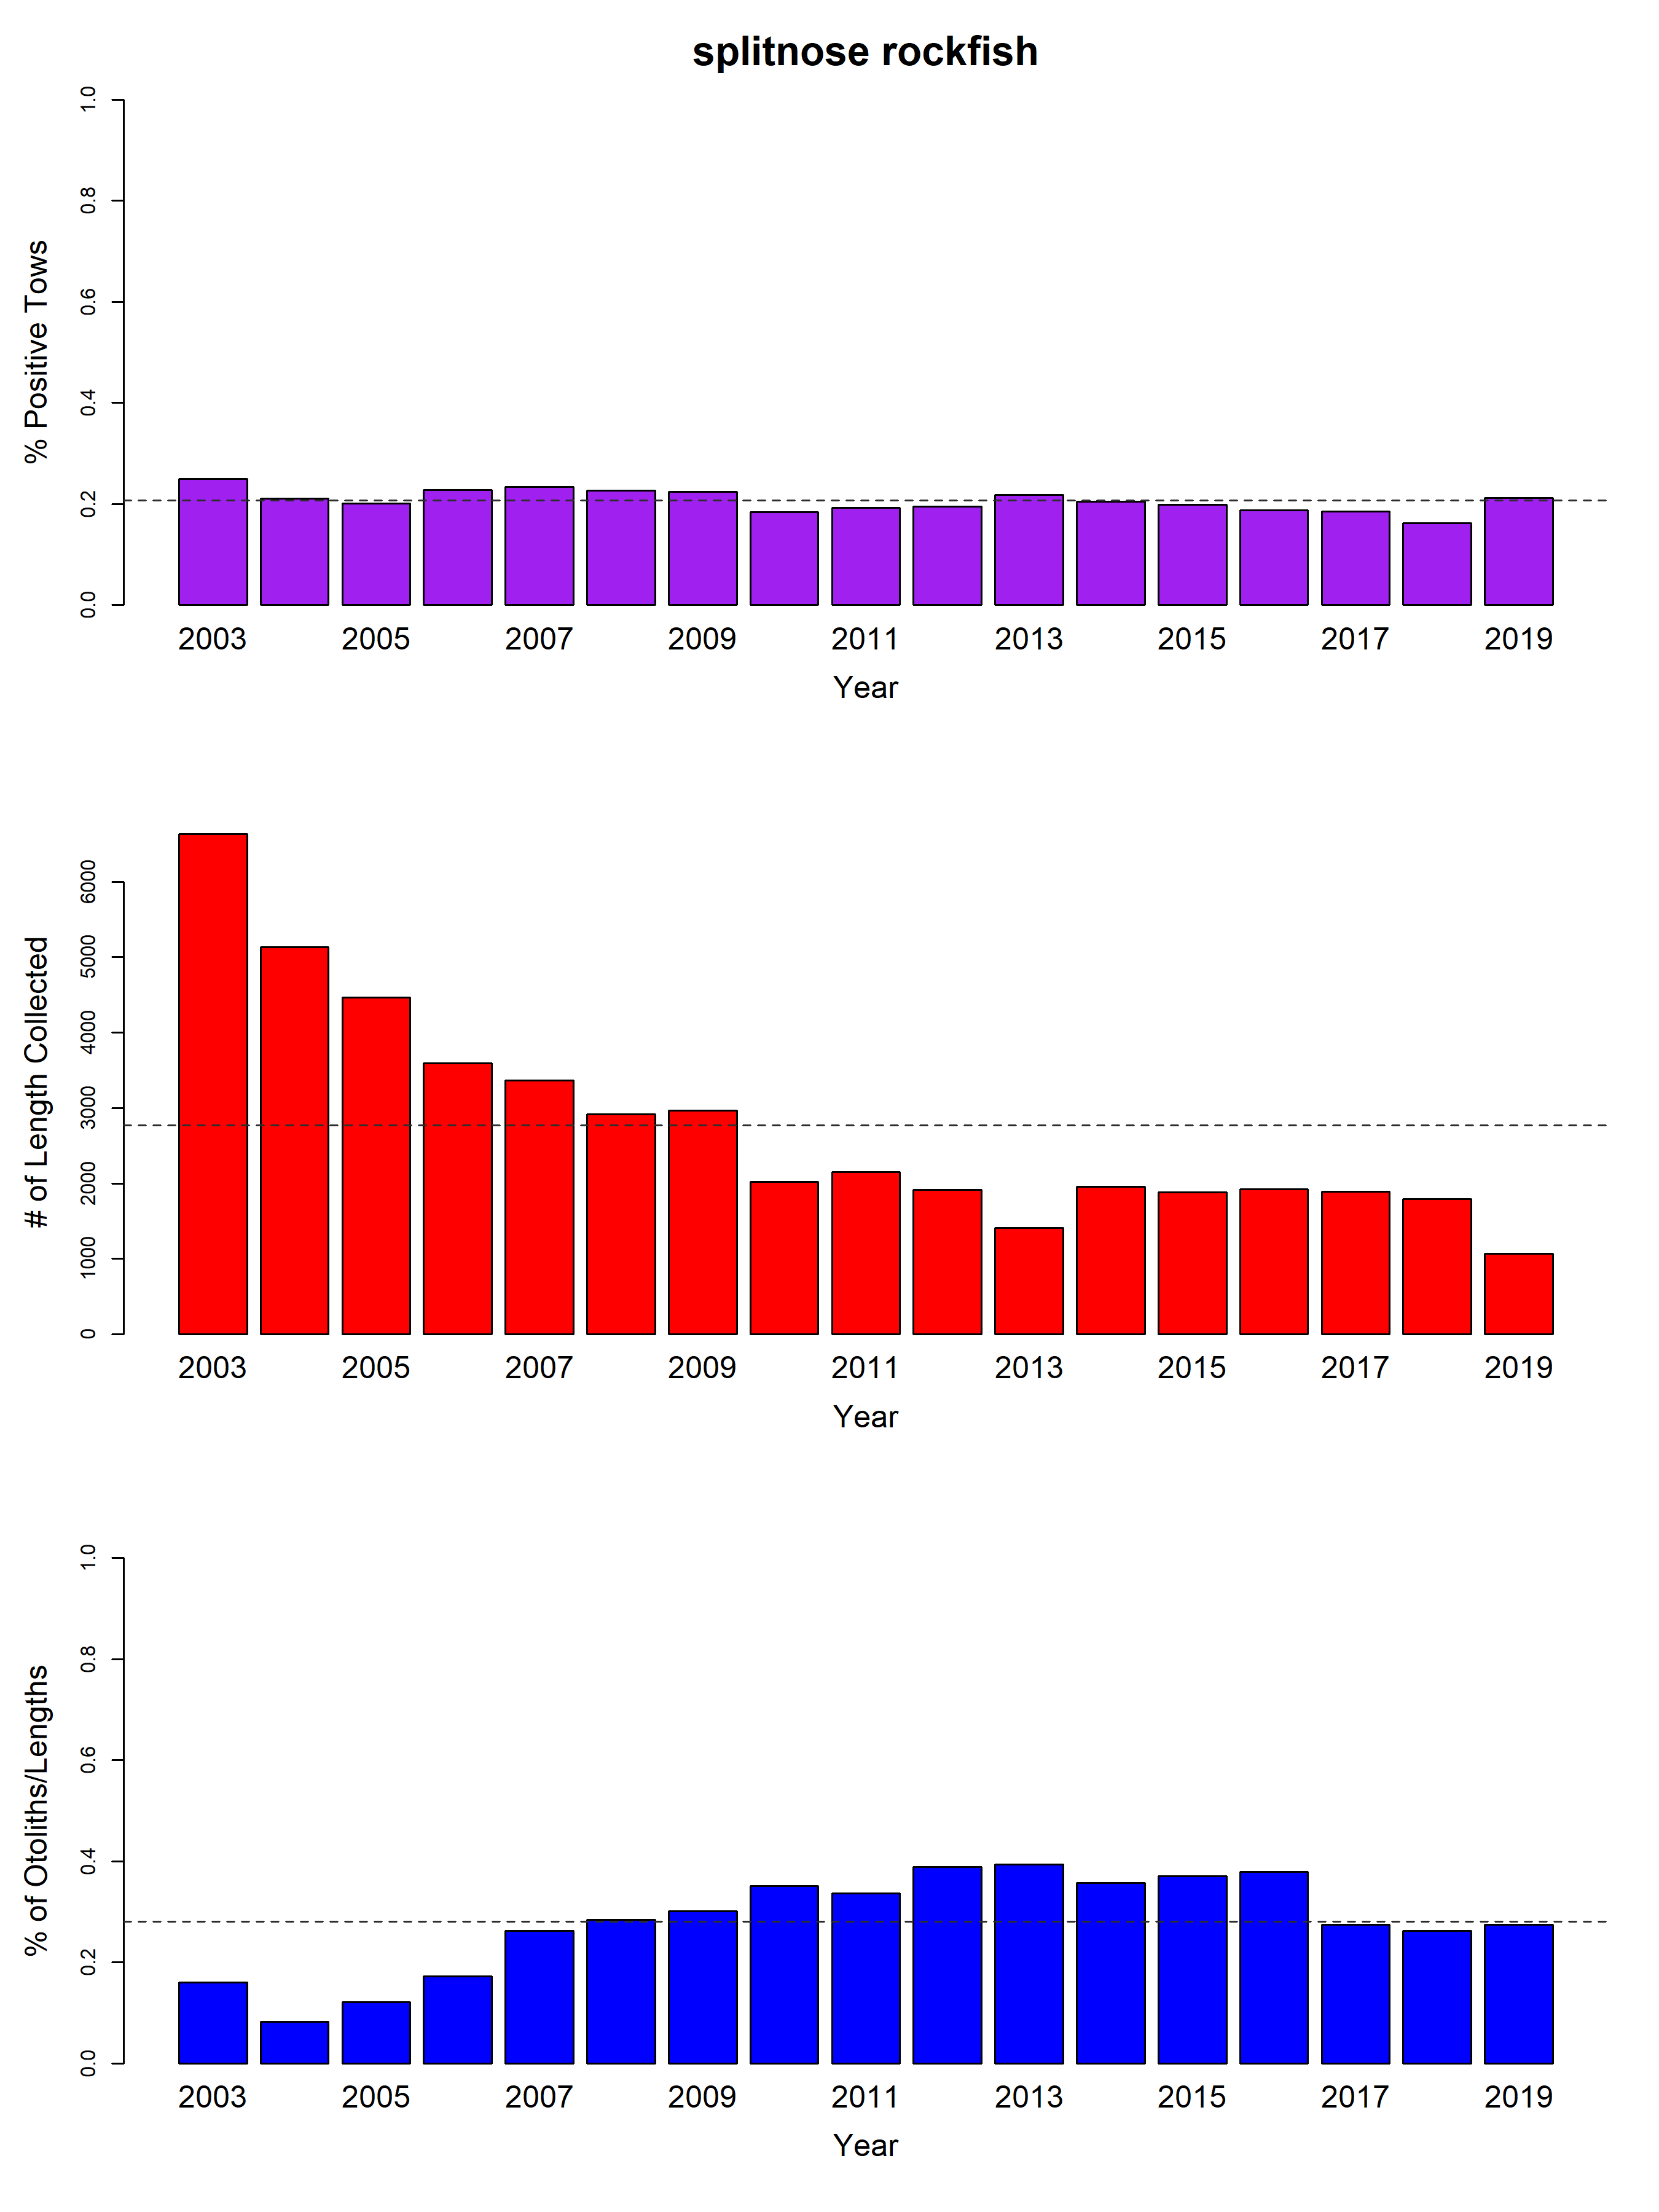
\includegraphics[width=0.6\textwidth,height=\textheight]{C:/Assessments/2020/survey_summary/sum_plots/splitnose_rockfish_survey_stats.png}
\FloatBarrier  

\FloatBarrier

\FloatBarrier

\FloatBarrier

\FloatBarrier

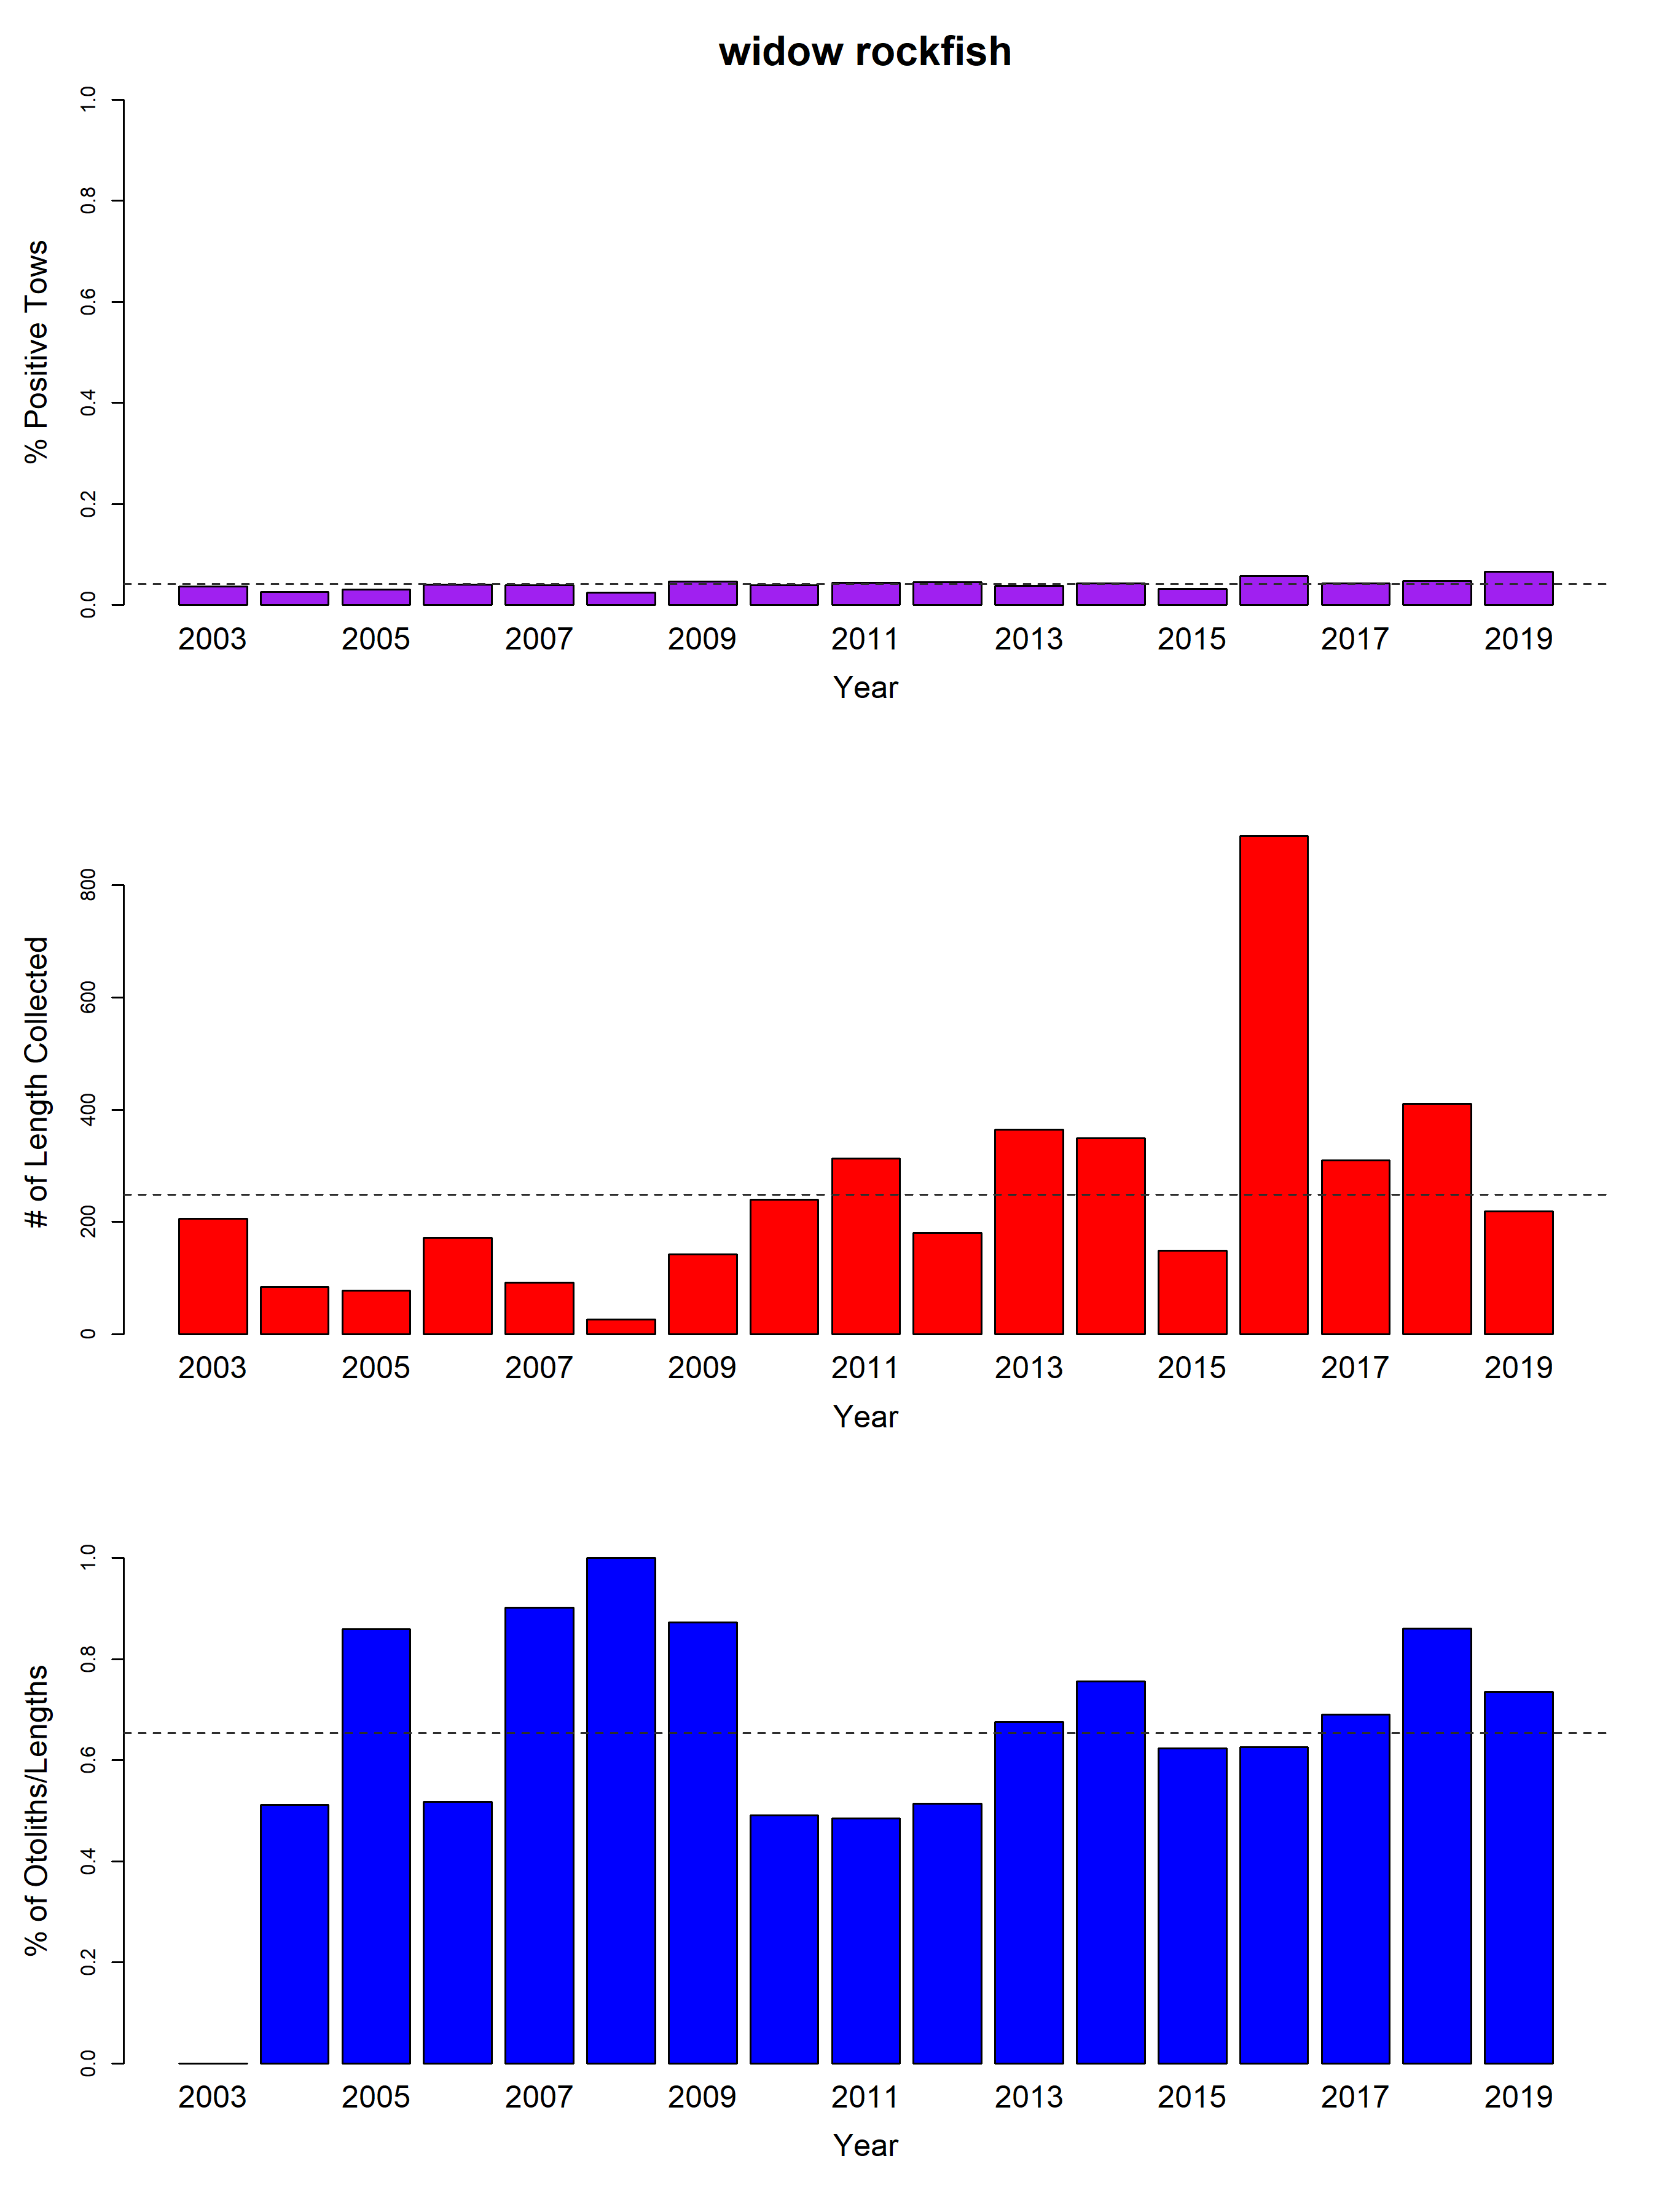
\includegraphics[width=0.6\textwidth,height=\textheight]{C:/Assessments/2020/survey_summary/sum_plots/widow_rockfish_survey_stats.png}
\FloatBarrier  

\FloatBarrier

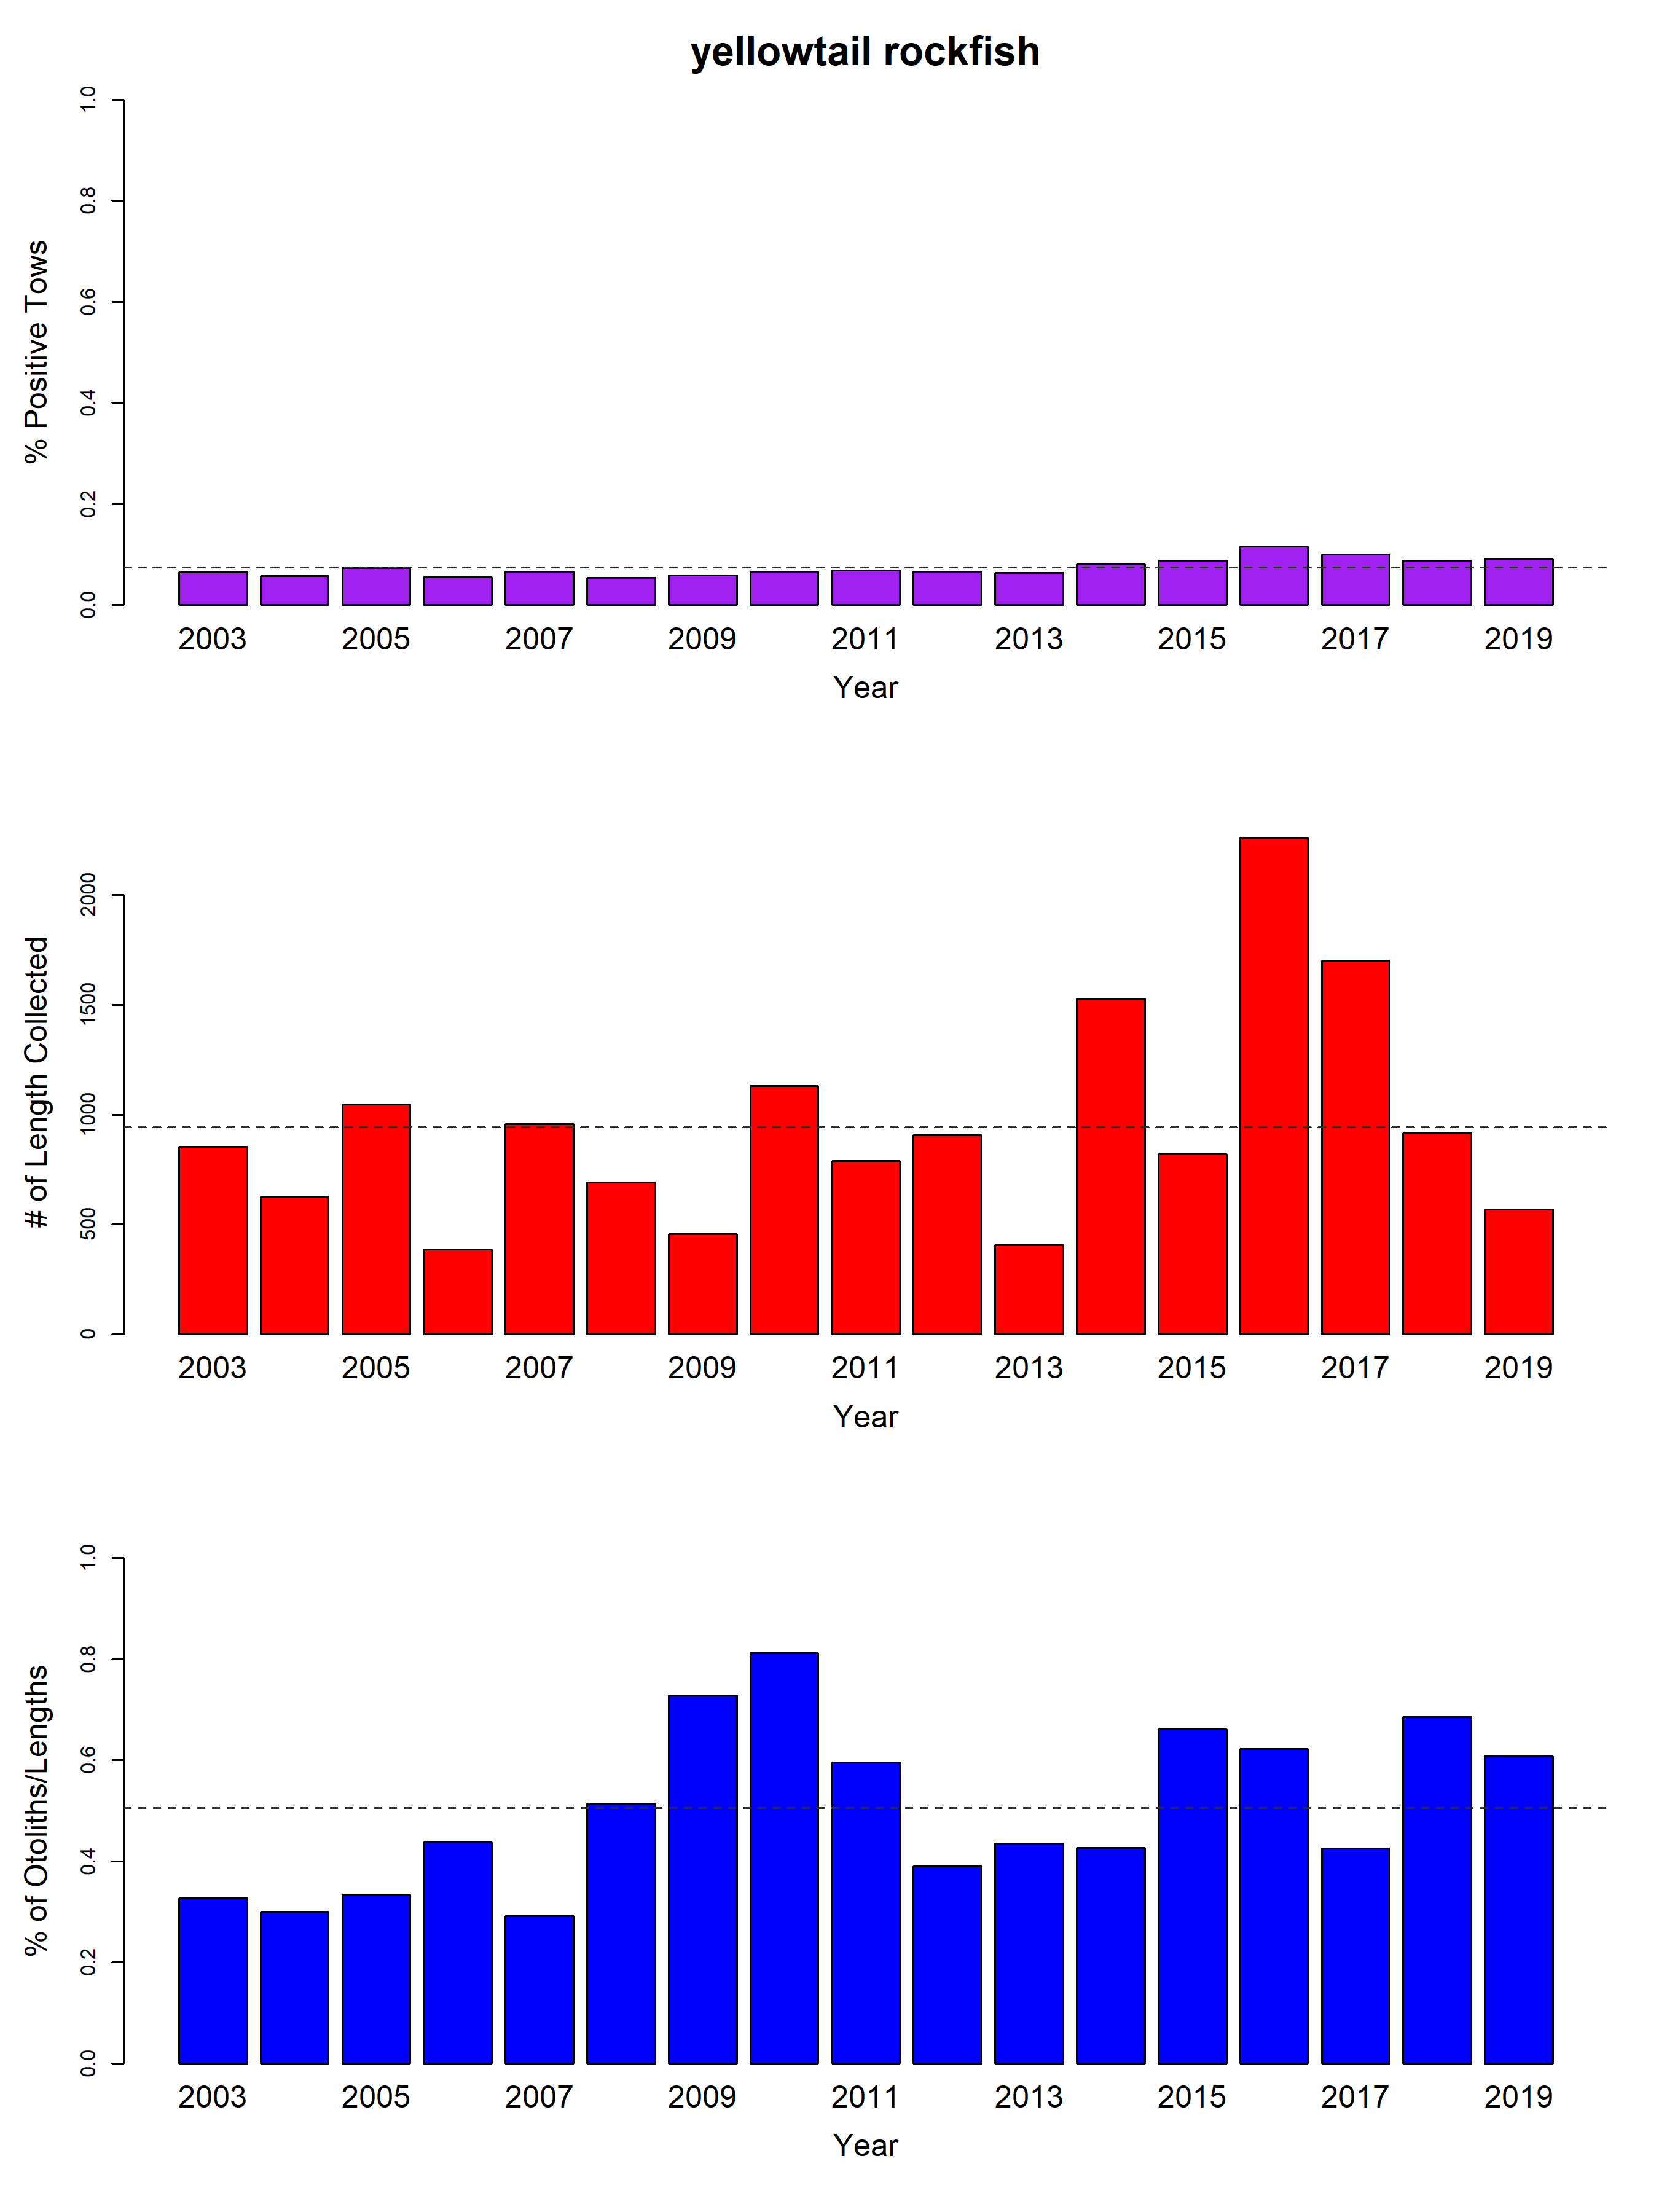
\includegraphics[width=0.6\textwidth,height=\textheight]{C:/Assessments/2020/survey_summary/sum_plots/yellowtail_rockfish_survey_stats.png}
\FloatBarrier  

\hypertarget{arrowtooth-flounder}{%
\subsection{Arrowtooth flounder}\label{arrowtooth-flounder}}

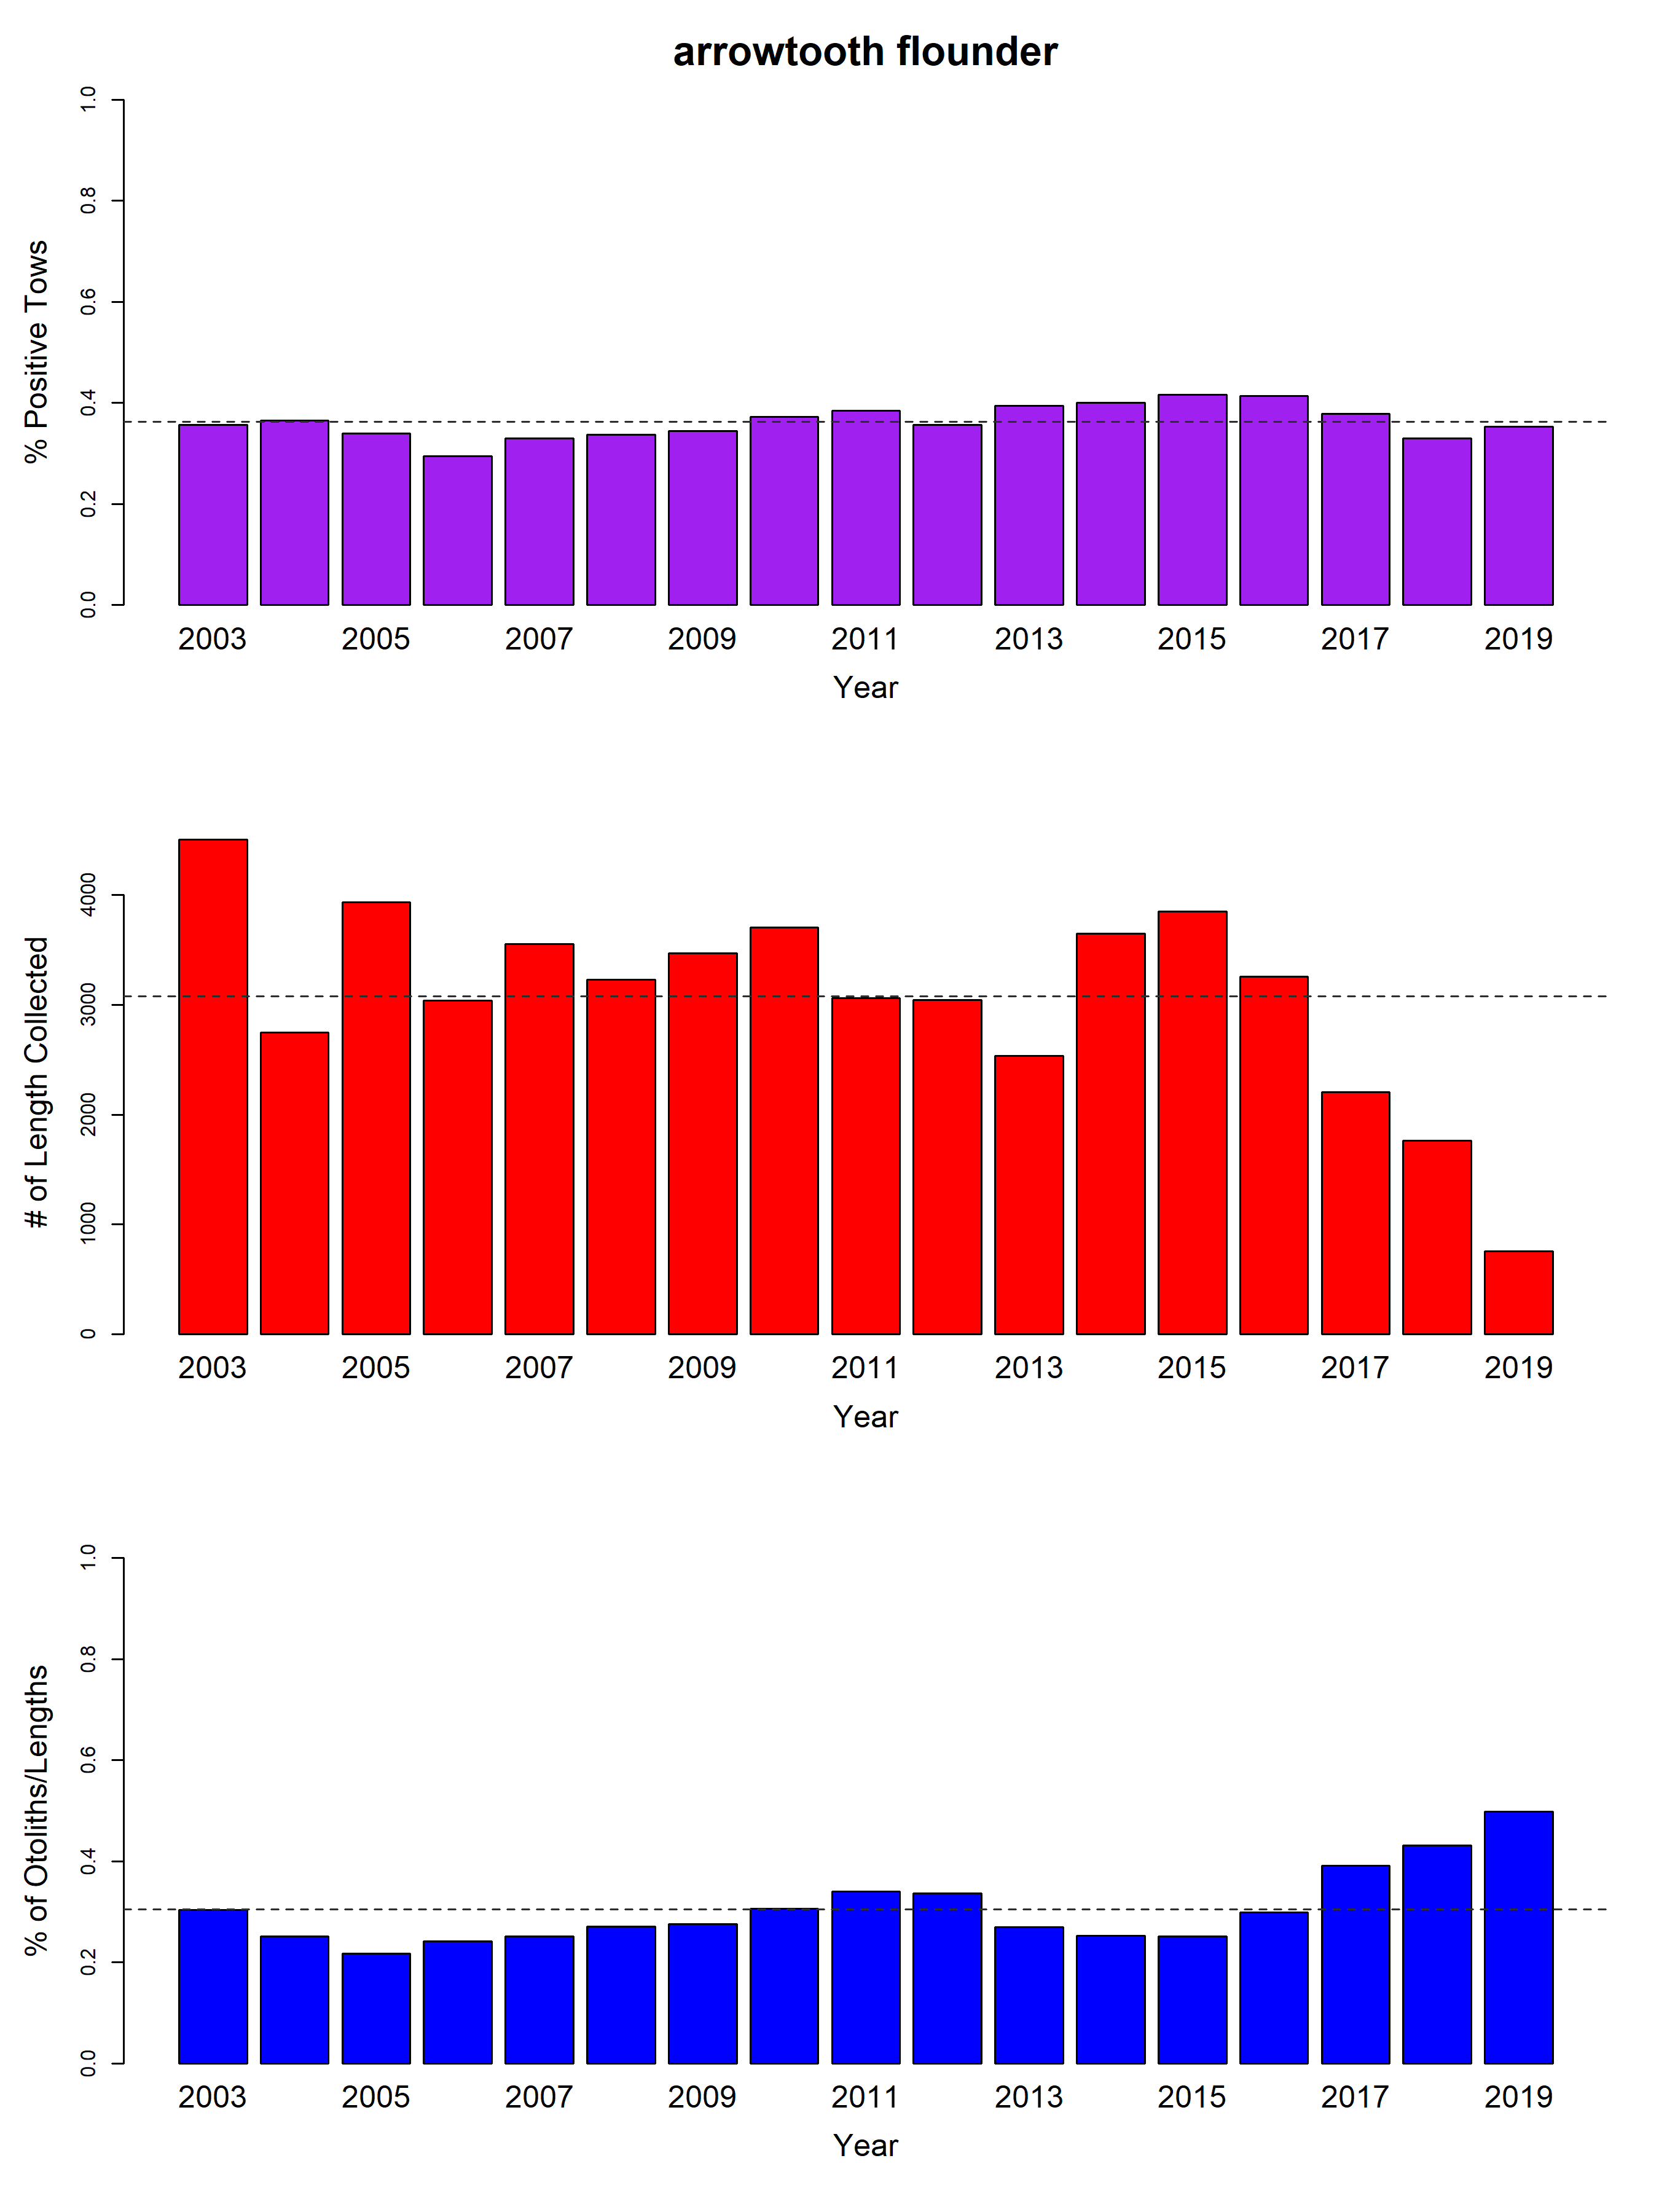
\includegraphics[width=0.6\textwidth,height=\textheight]{C:/Assessments/2020/survey_summary/sum_plots/arrowtooth_flounder_survey_stats.png}
\FloatBarrier  

\hypertarget{aurora-rockfish}{%
\subsection{Aurora rockfish}\label{aurora-rockfish}}

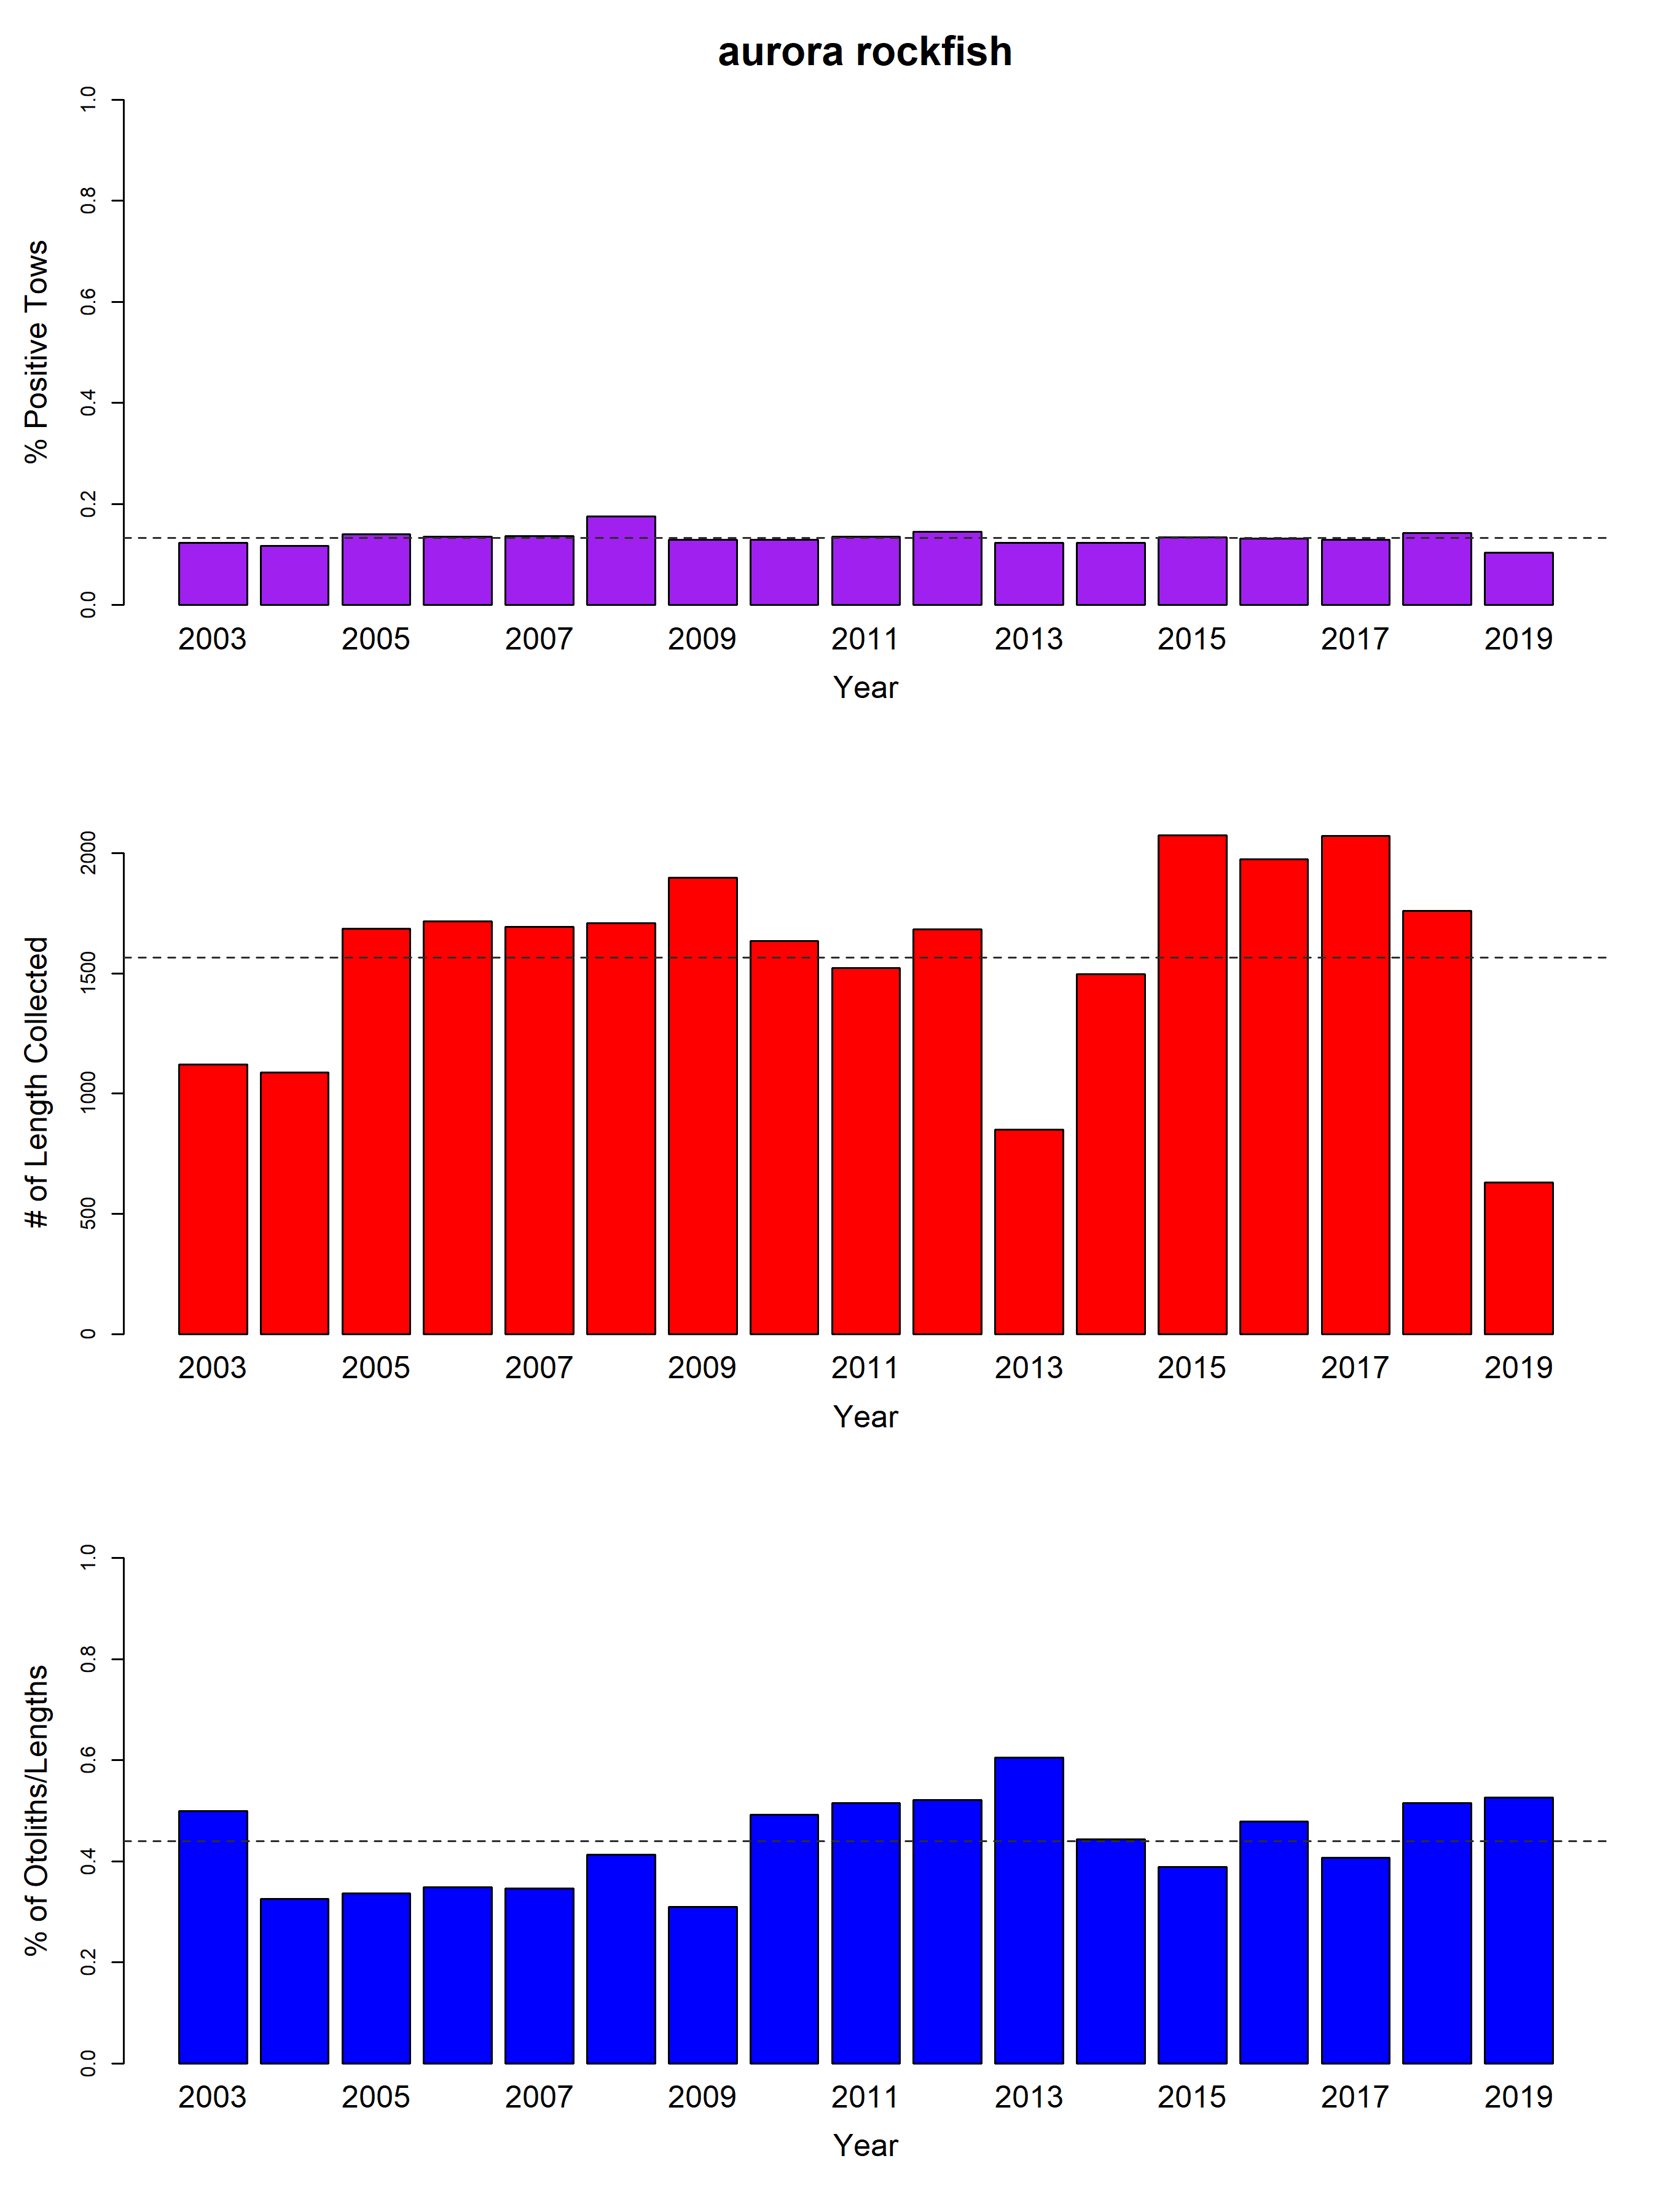
\includegraphics[width=0.6\textwidth,height=\textheight]{C:/Assessments/2020/survey_summary/sum_plots/aurora_rockfish_survey_stats.png}
\FloatBarrier  

\hypertarget{bank-rockfish}{%
\subsection{Bank rockfish}\label{bank-rockfish}}

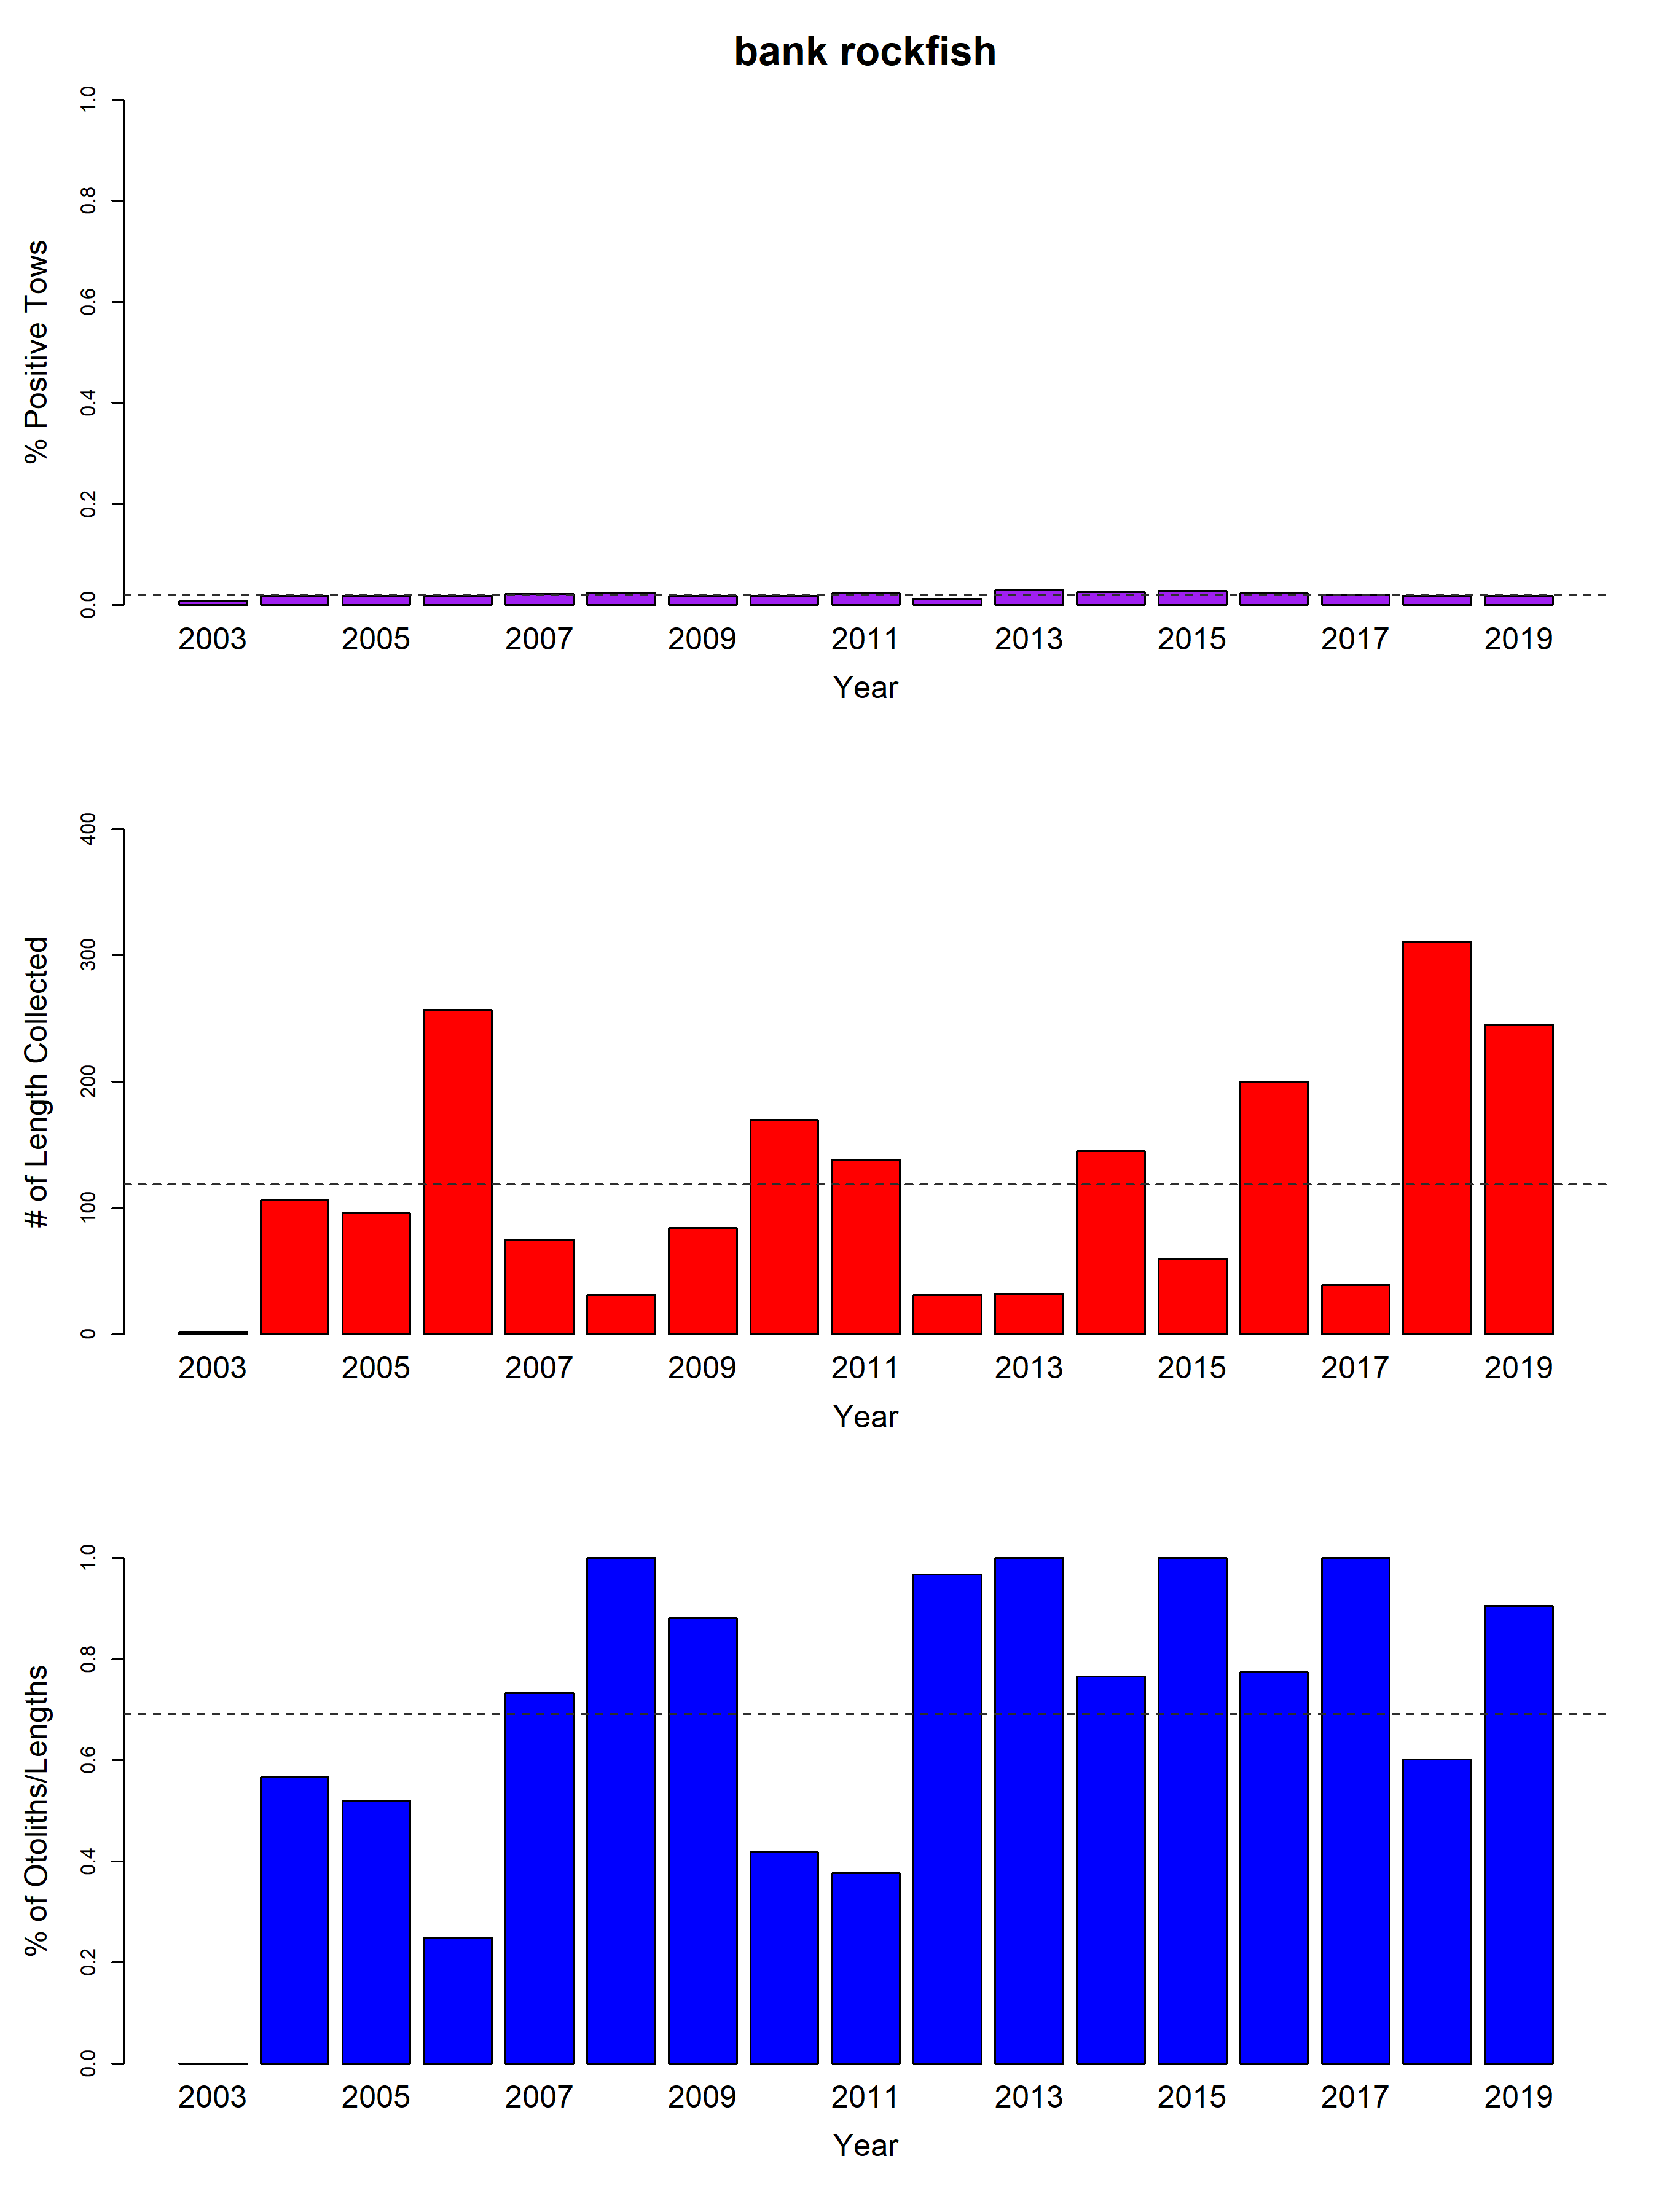
\includegraphics[width=0.6\textwidth,height=\textheight]{C:/Assessments/2020/survey_summary/sum_plots/bank_rockfish_survey_stats.png}
\FloatBarrier  

\hypertarget{big-skate}{%
\subsection{Big skate}\label{big-skate}}

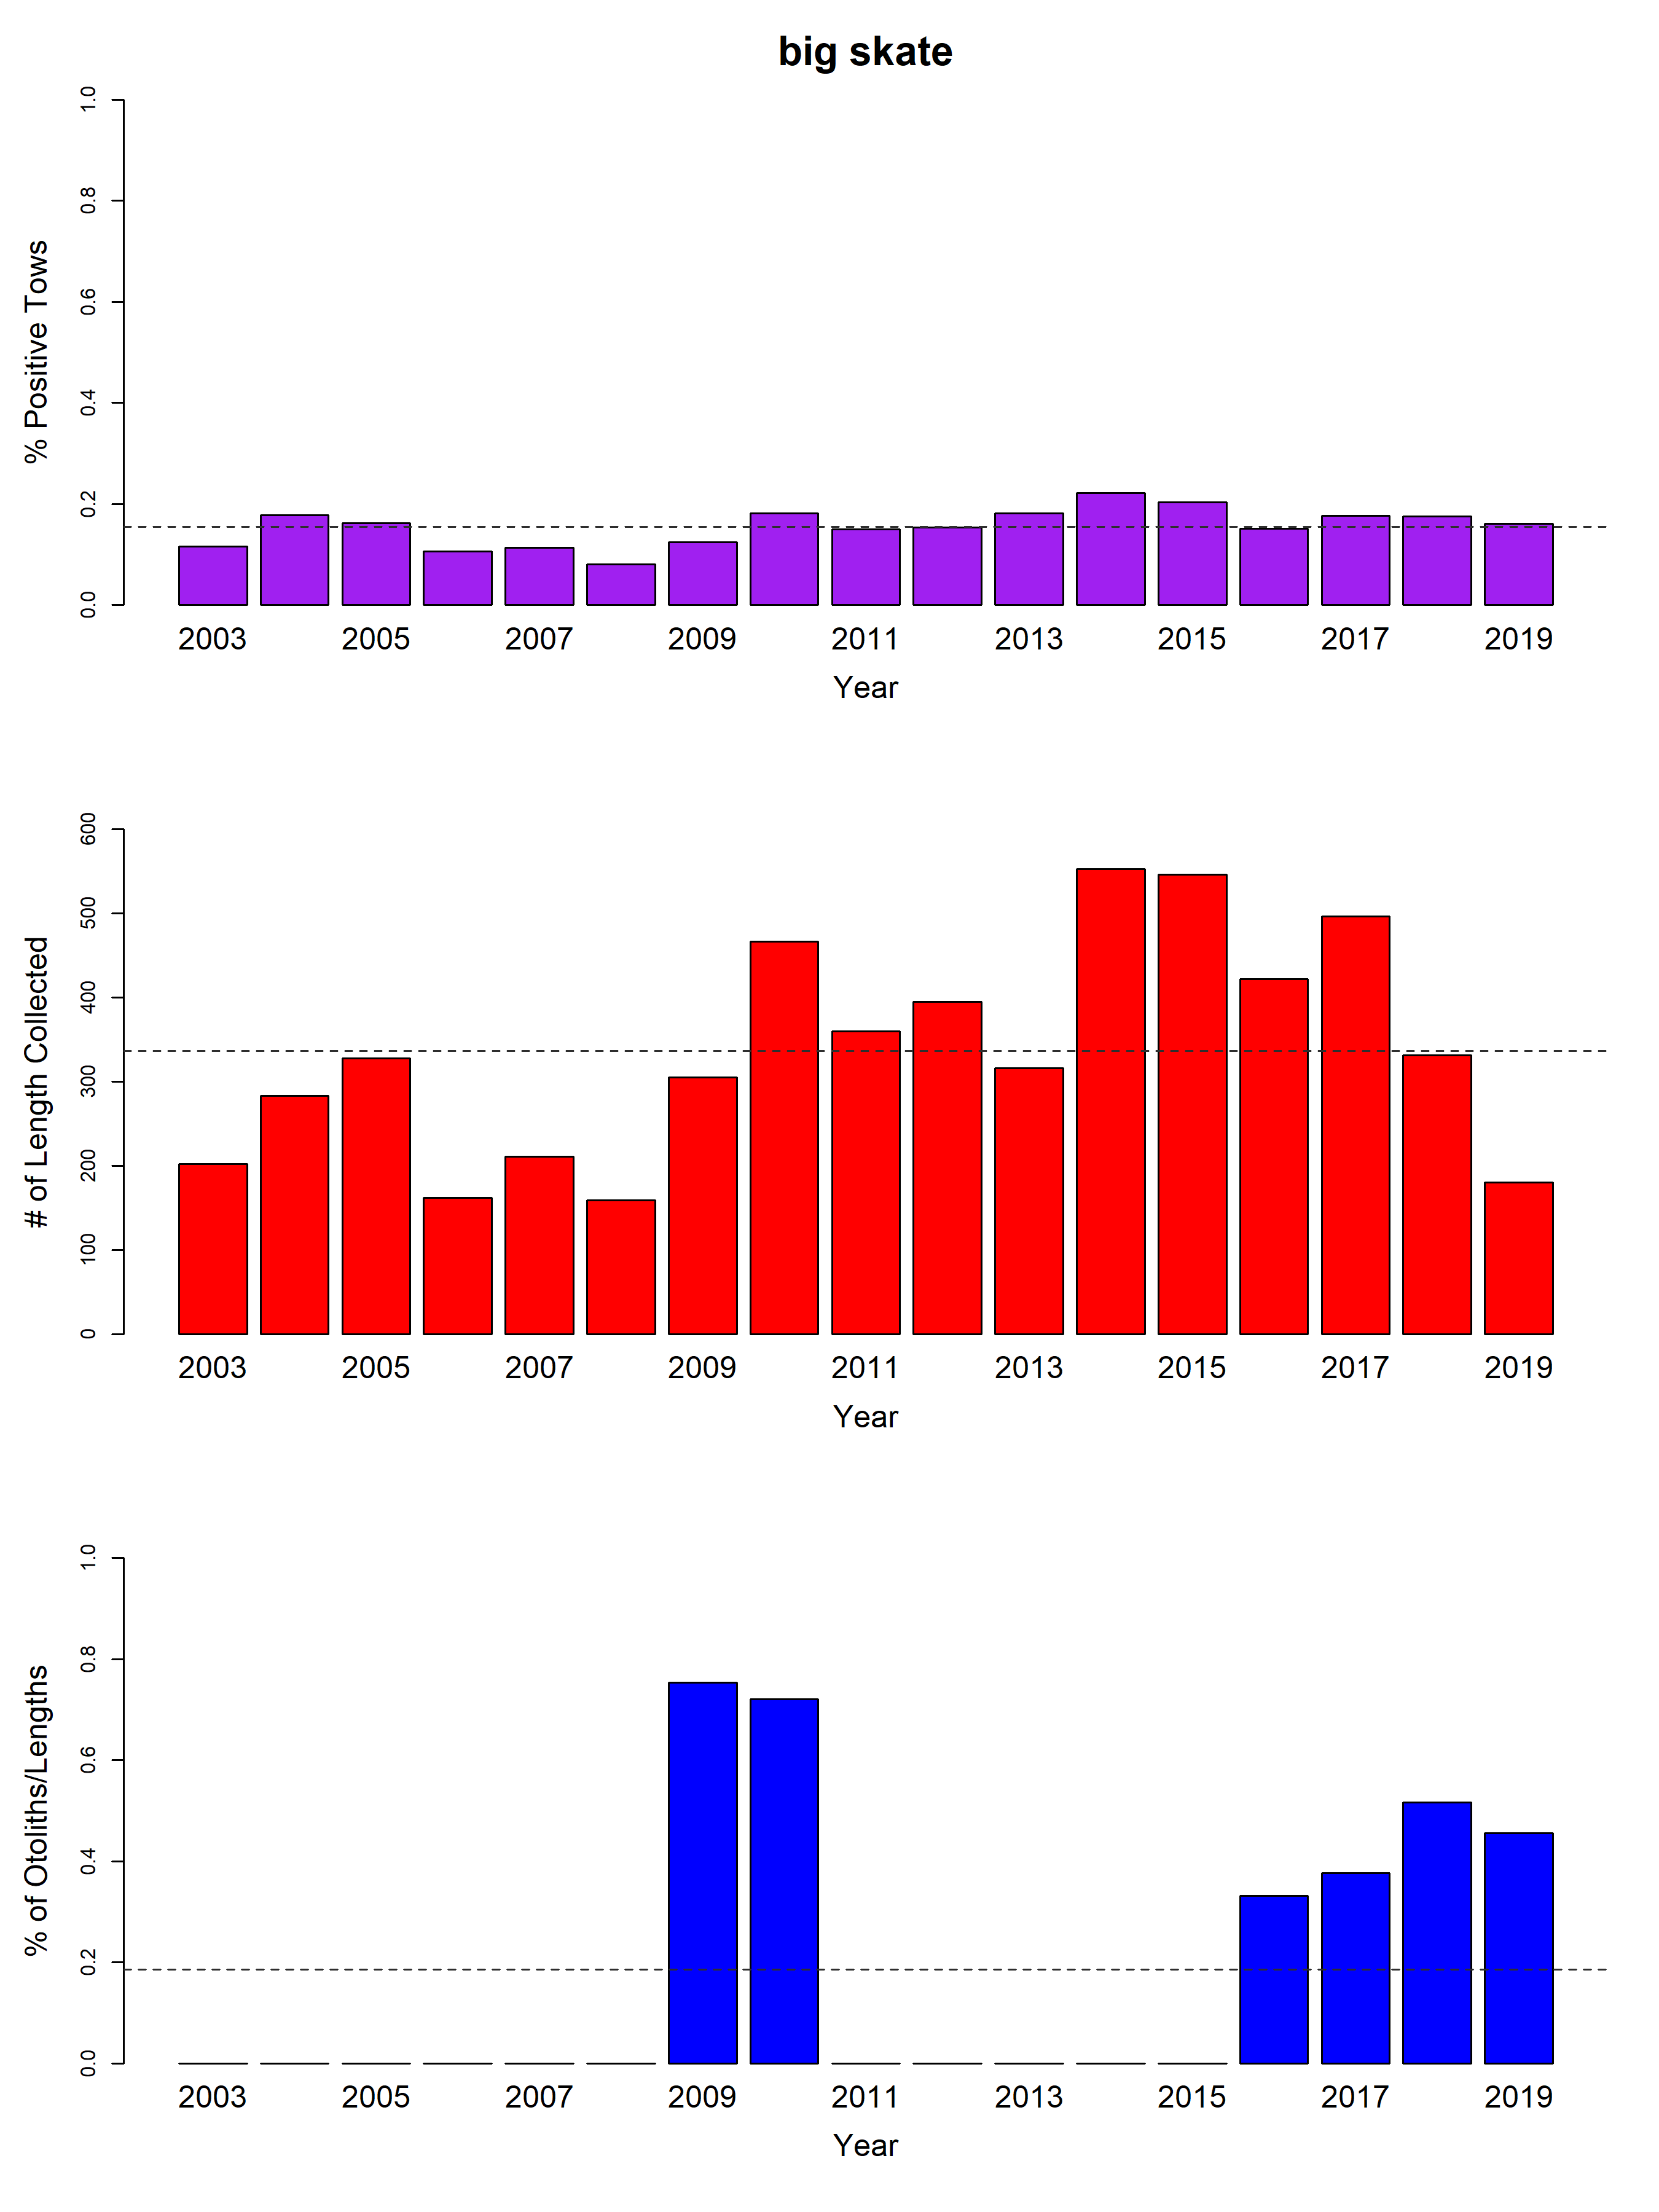
\includegraphics[width=0.6\textwidth,height=\textheight]{C:/Assessments/2020/survey_summary/sum_plots/big_skate_survey_stats.png}
\FloatBarrier  

\hypertarget{blackgill-rockfish}{%
\subsection{Blackgill rockfish}\label{blackgill-rockfish}}

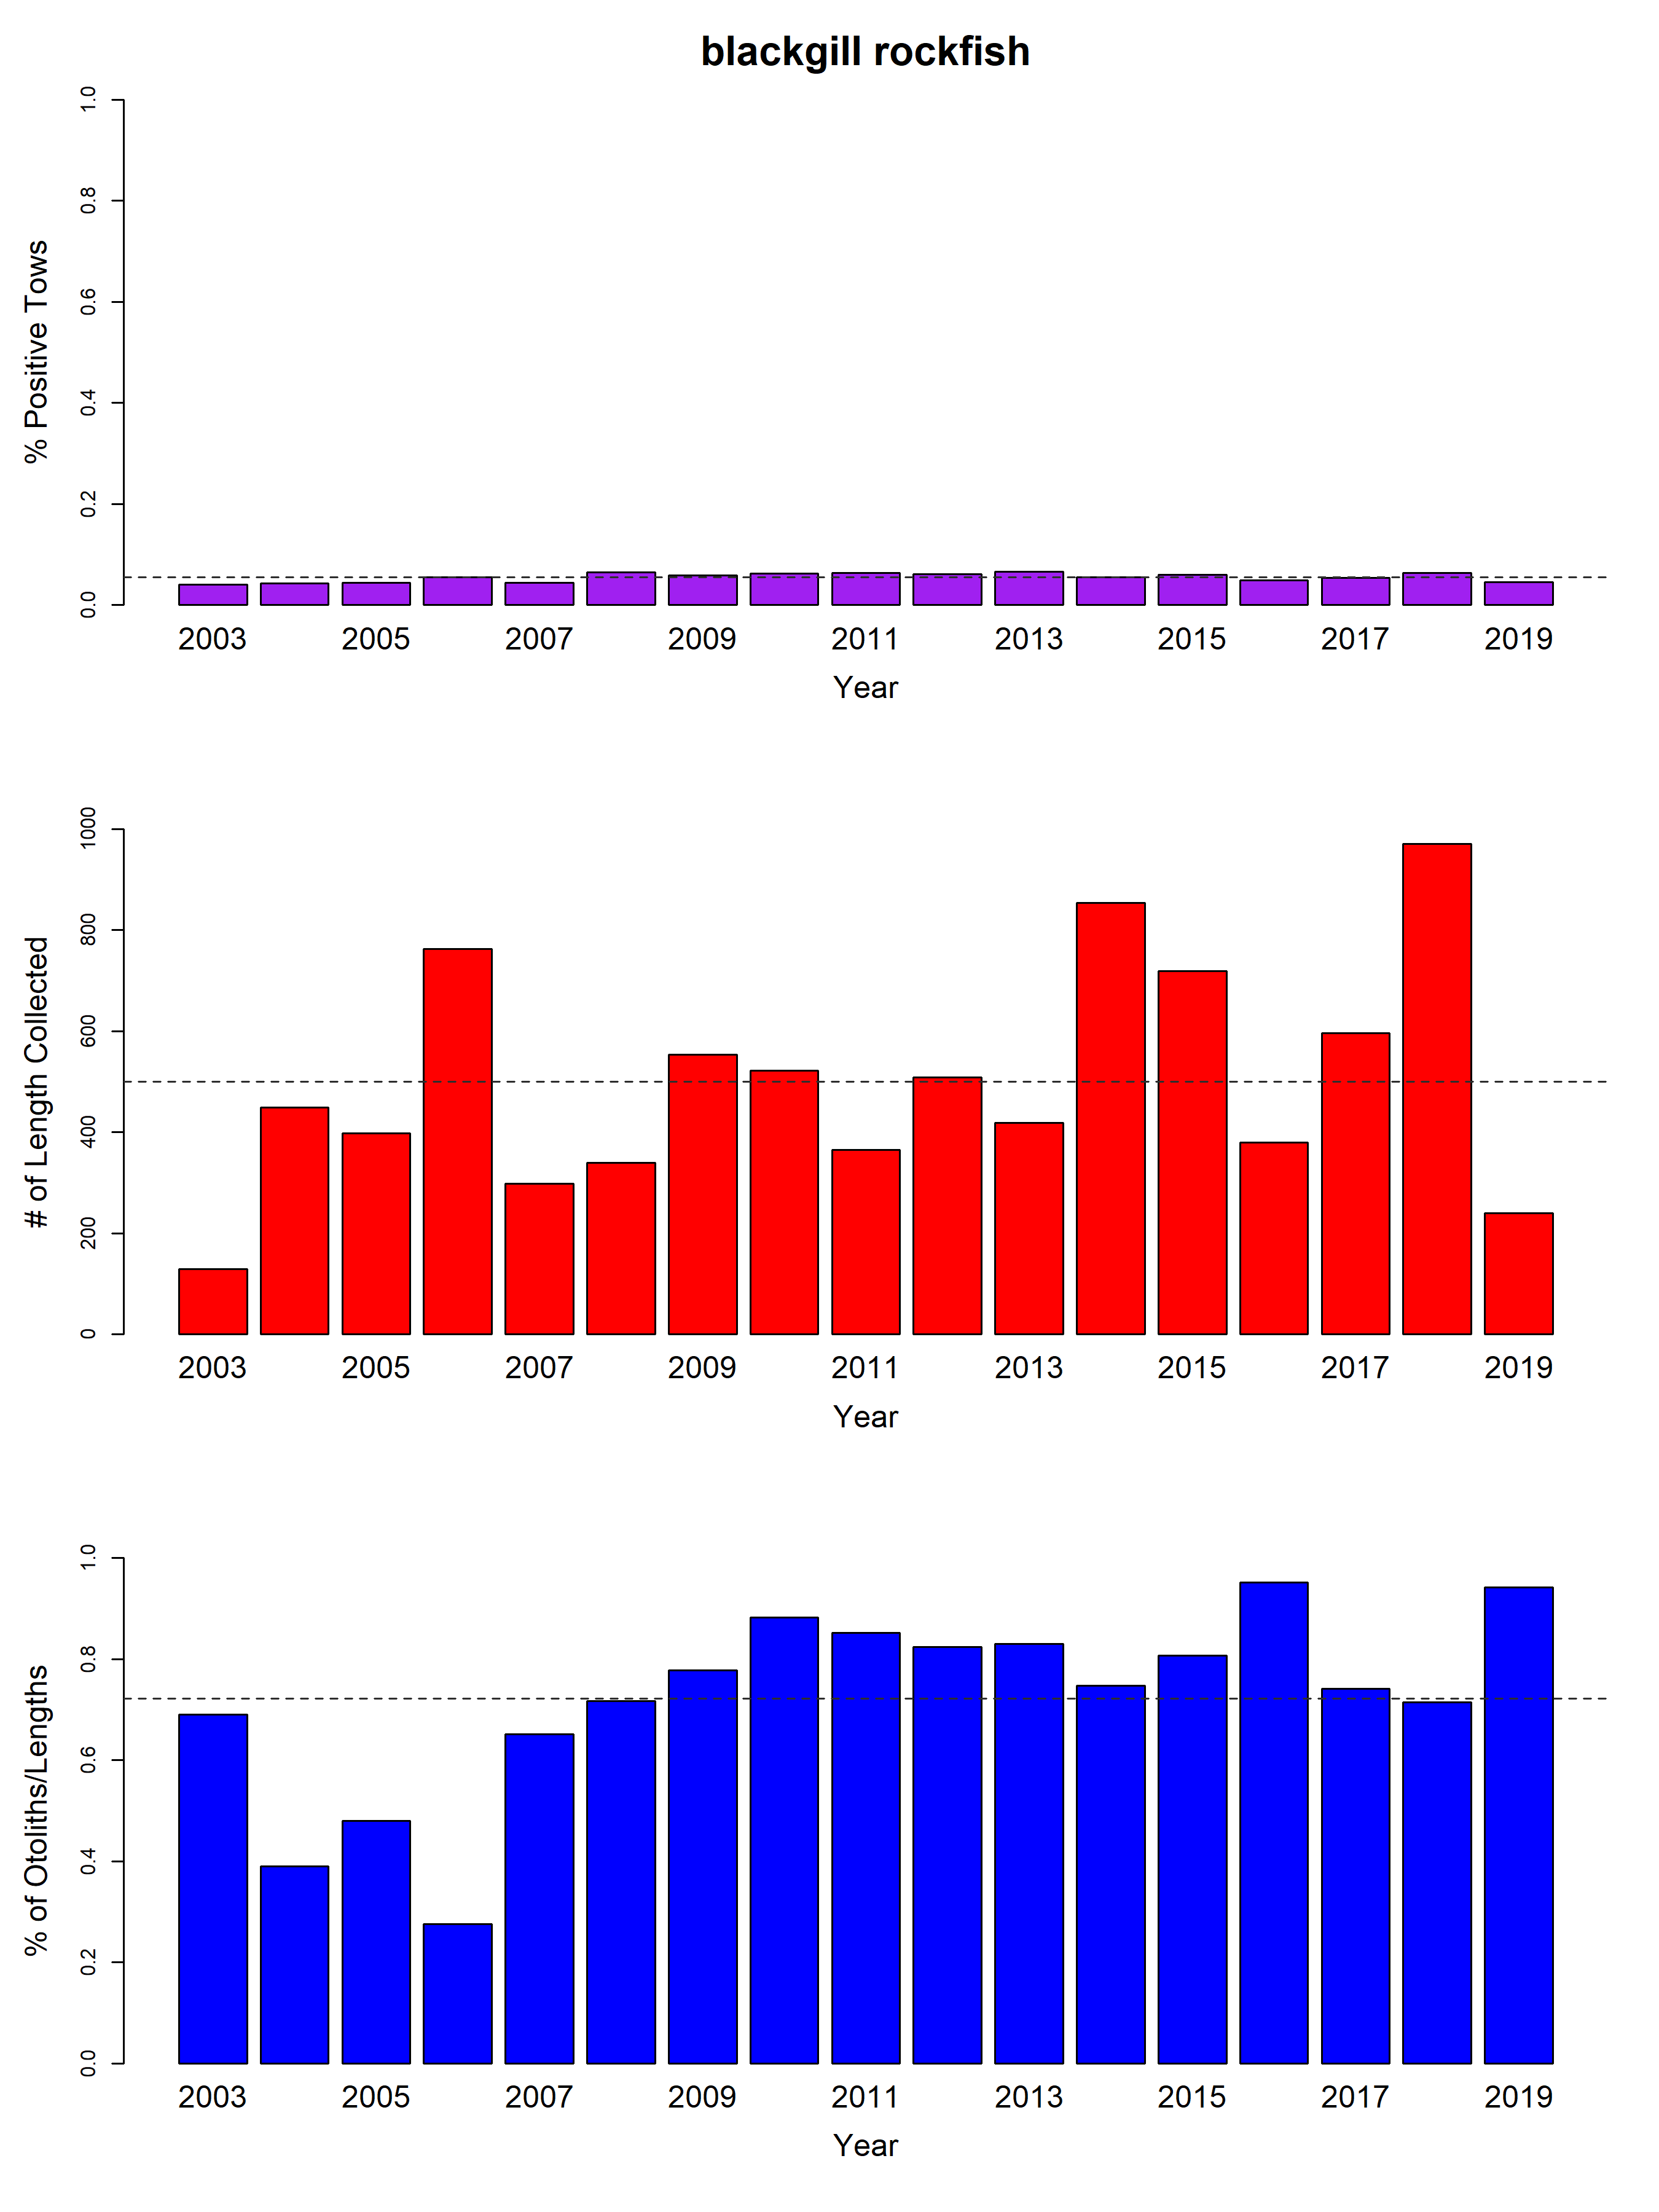
\includegraphics[width=0.6\textwidth,height=\textheight]{C:/Assessments/2020/survey_summary/sum_plots/blackgill_rockfish_survey_stats.png}
\FloatBarrier  

\hypertarget{blue-rockfish}{%
\subsection{Blue rockfish}\label{blue-rockfish}}

\FloatBarrier

\hypertarget{bocaccio}{%
\subsection{Bocaccio}\label{bocaccio}}

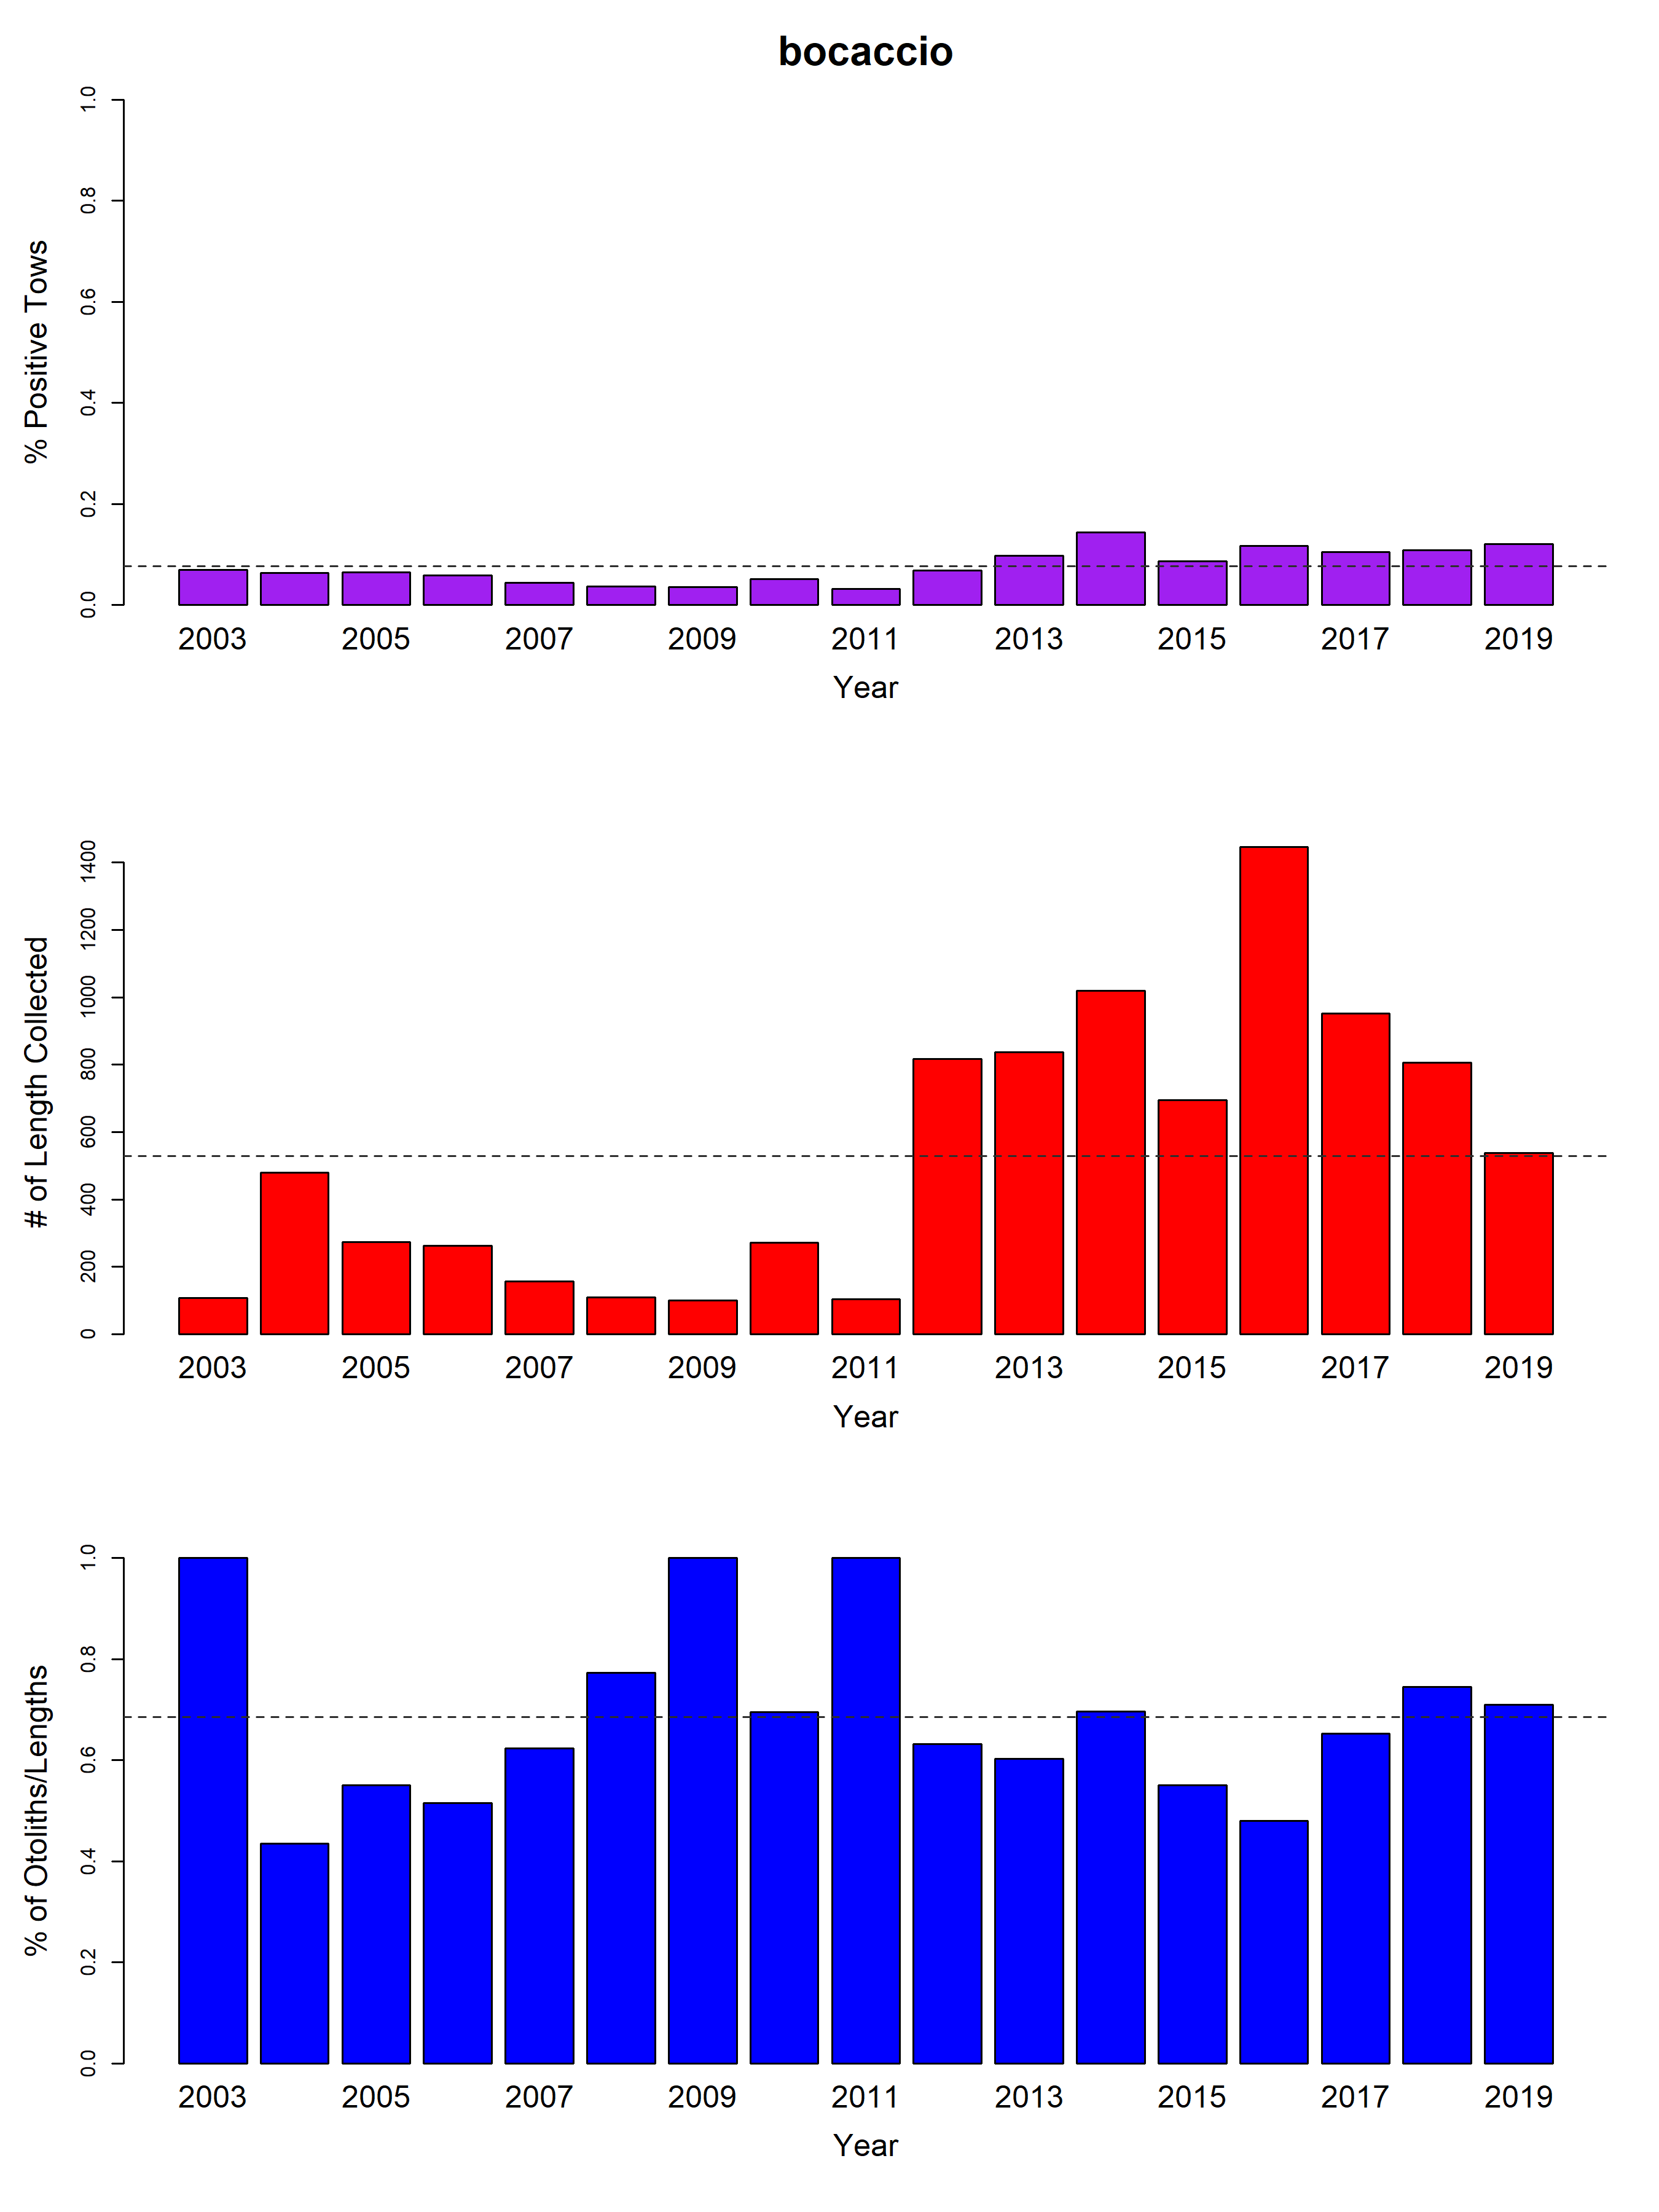
\includegraphics[width=0.6\textwidth,height=\textheight]{C:/Assessments/2020/survey_summary/sum_plots/bocaccio_survey_stats.png}
\FloatBarrier  

\hypertarget{brown-rockfish}{%
\subsection{Brown rockfish}\label{brown-rockfish}}

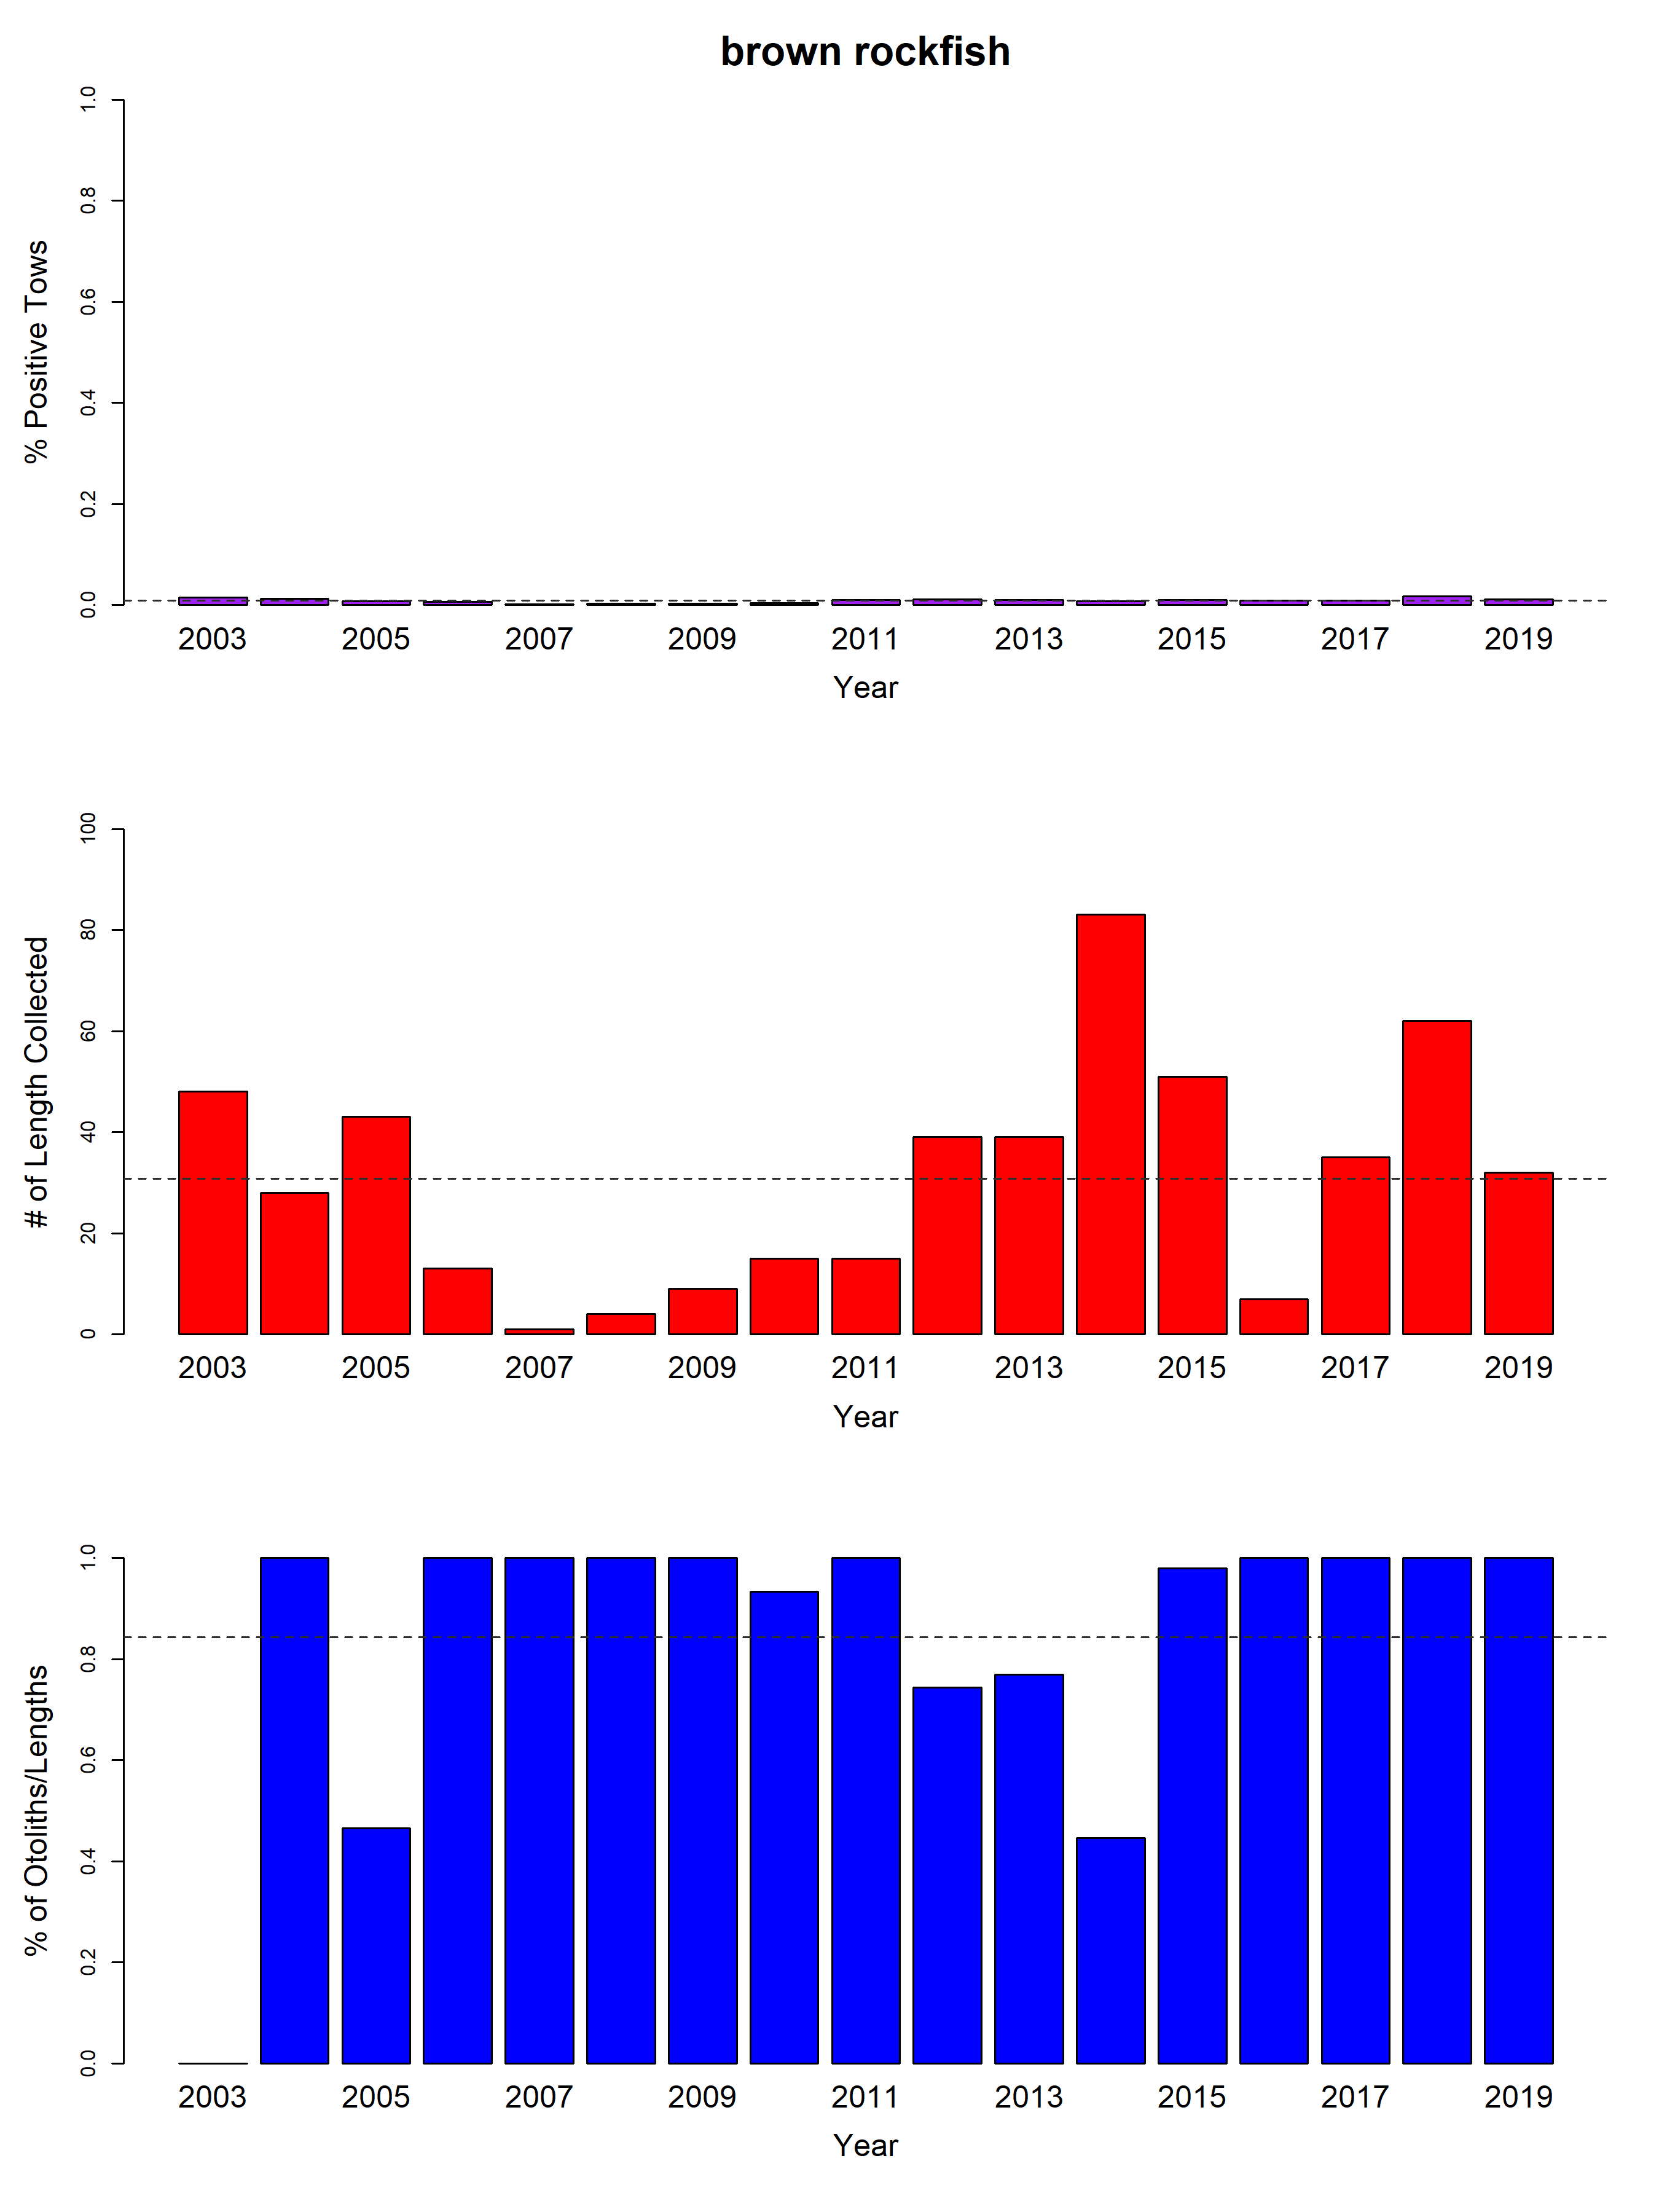
\includegraphics[width=0.6\textwidth,height=\textheight]{C:/Assessments/2020/survey_summary/sum_plots/brown_rockfish_survey_stats.png}
\FloatBarrier  

\hypertarget{canary-rockfish}{%
\subsection{Canary rockfish}\label{canary-rockfish}}

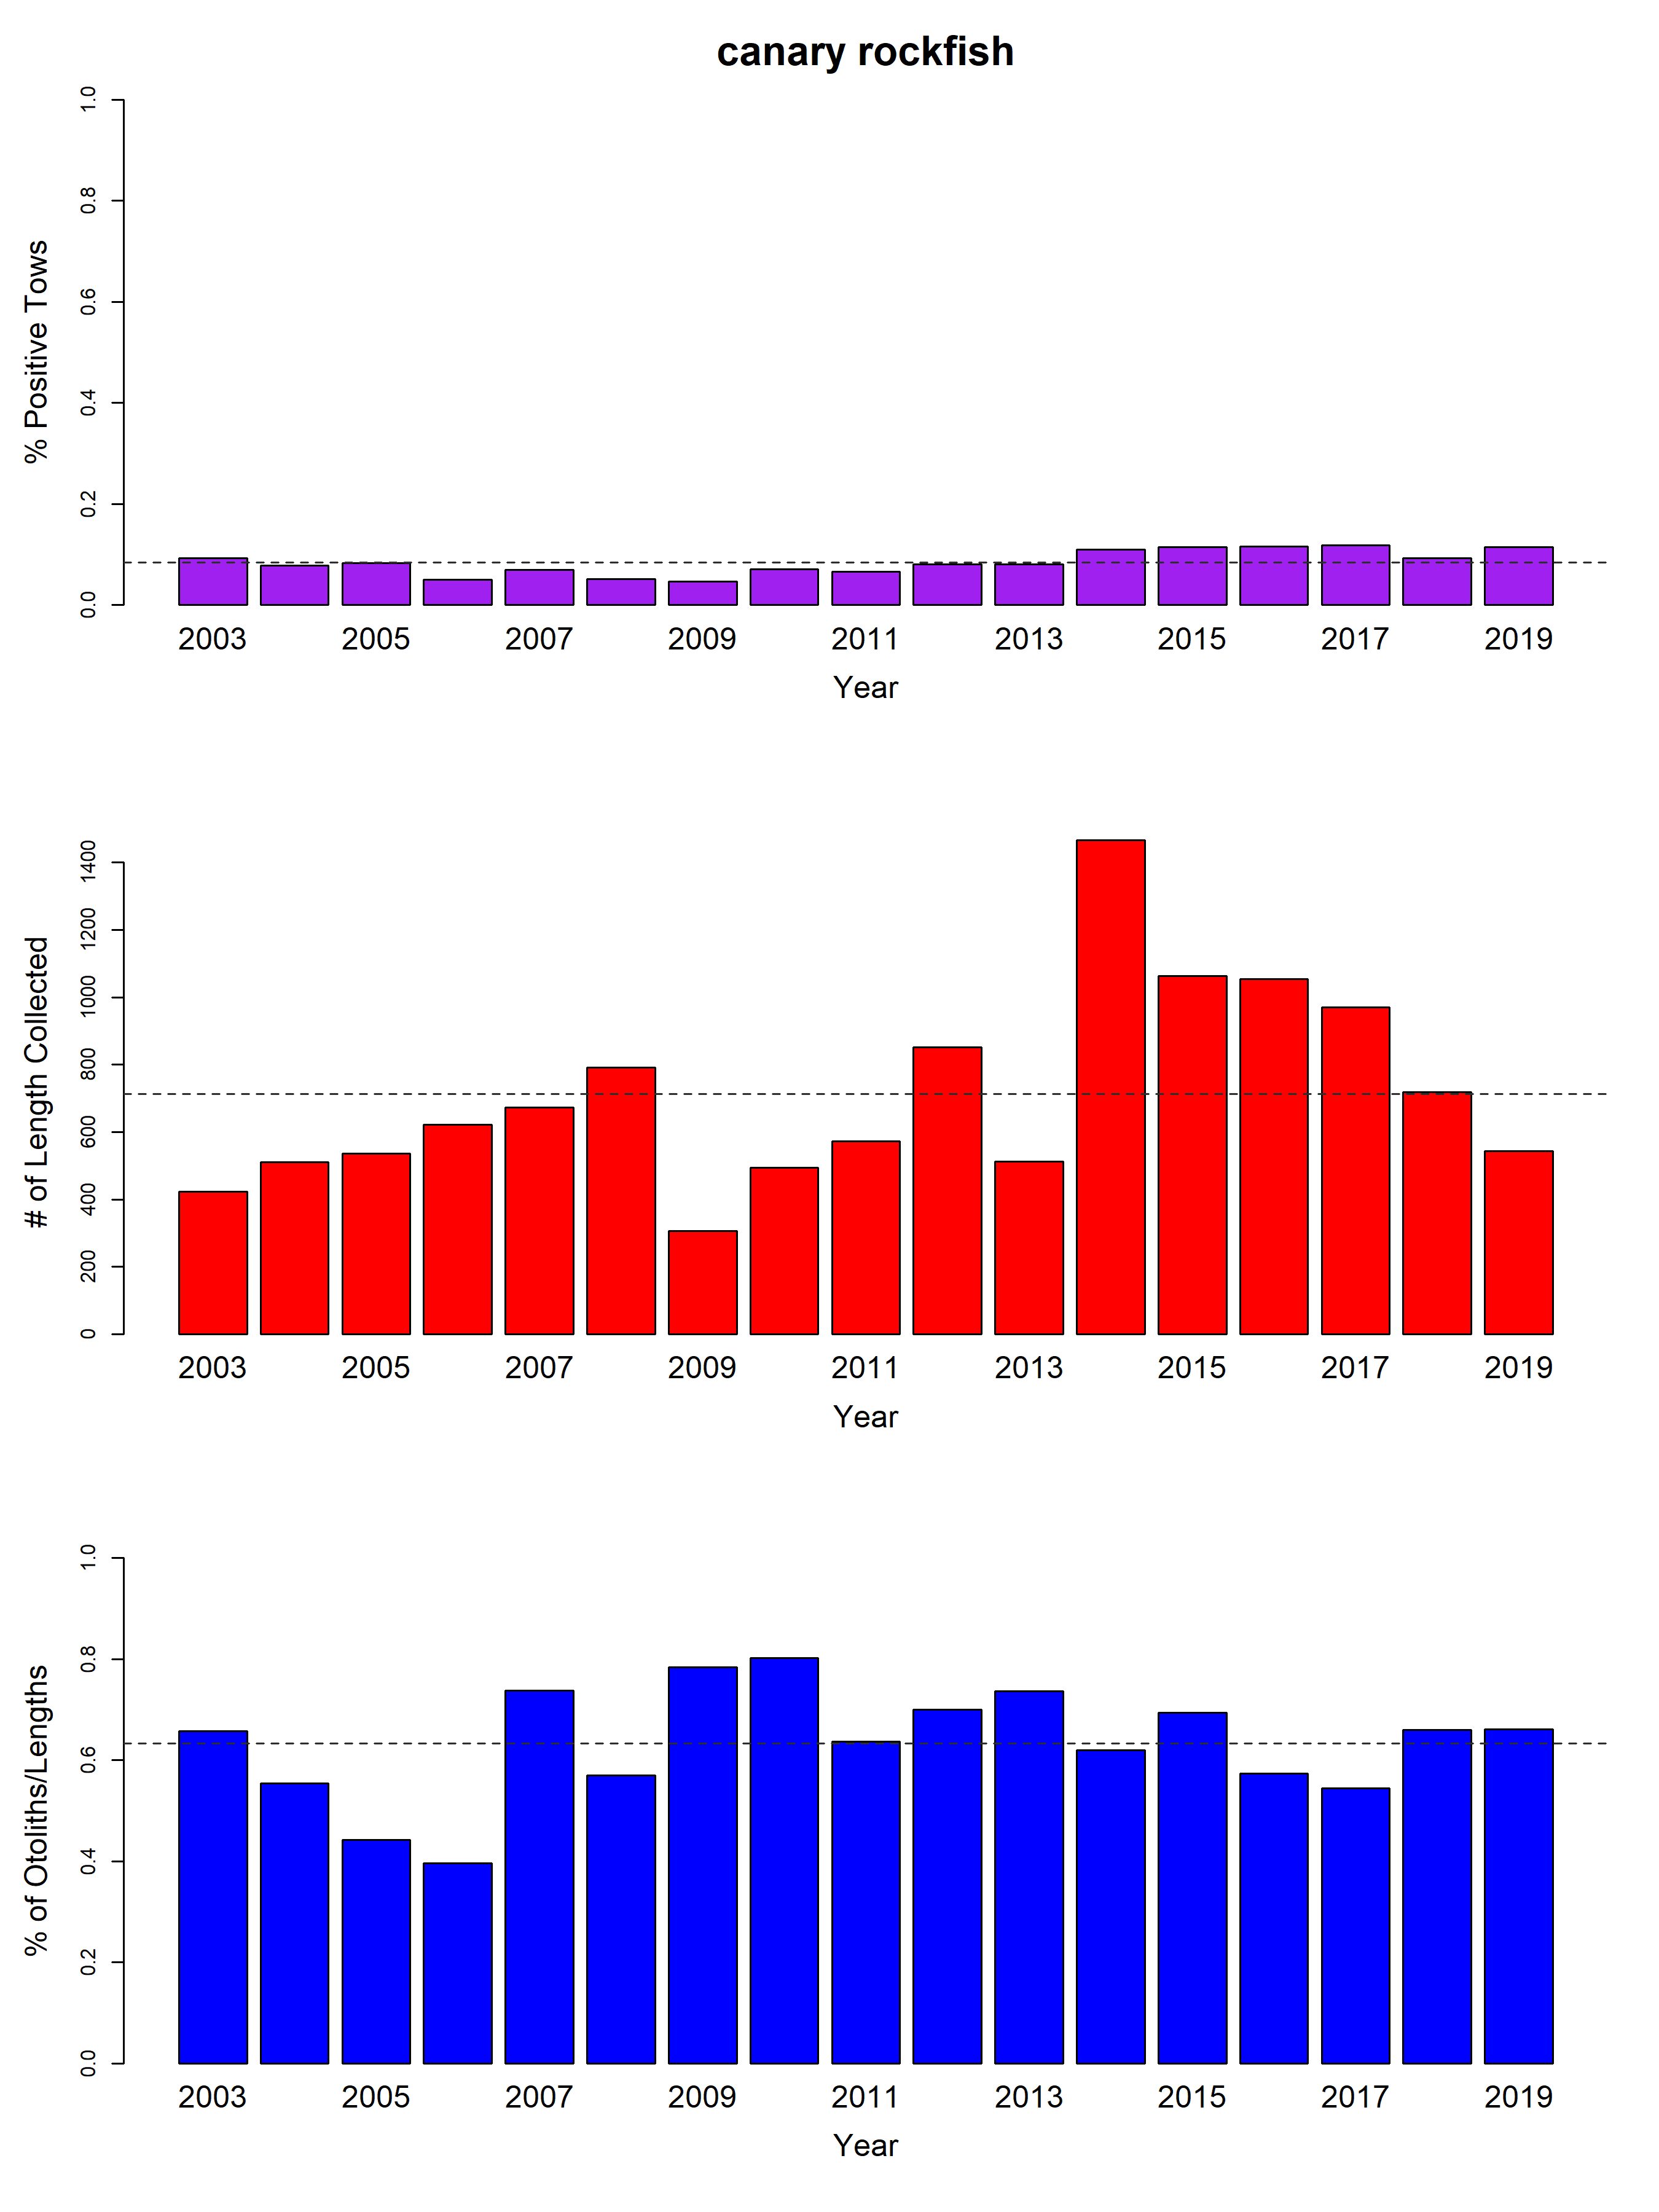
\includegraphics[width=0.6\textwidth,height=\textheight]{C:/Assessments/2020/survey_summary/sum_plots/canary_rockfish_survey_stats.png}
\FloatBarrier  

\hypertarget{chilipepper}{%
\subsection{Chilipepper}\label{chilipepper}}

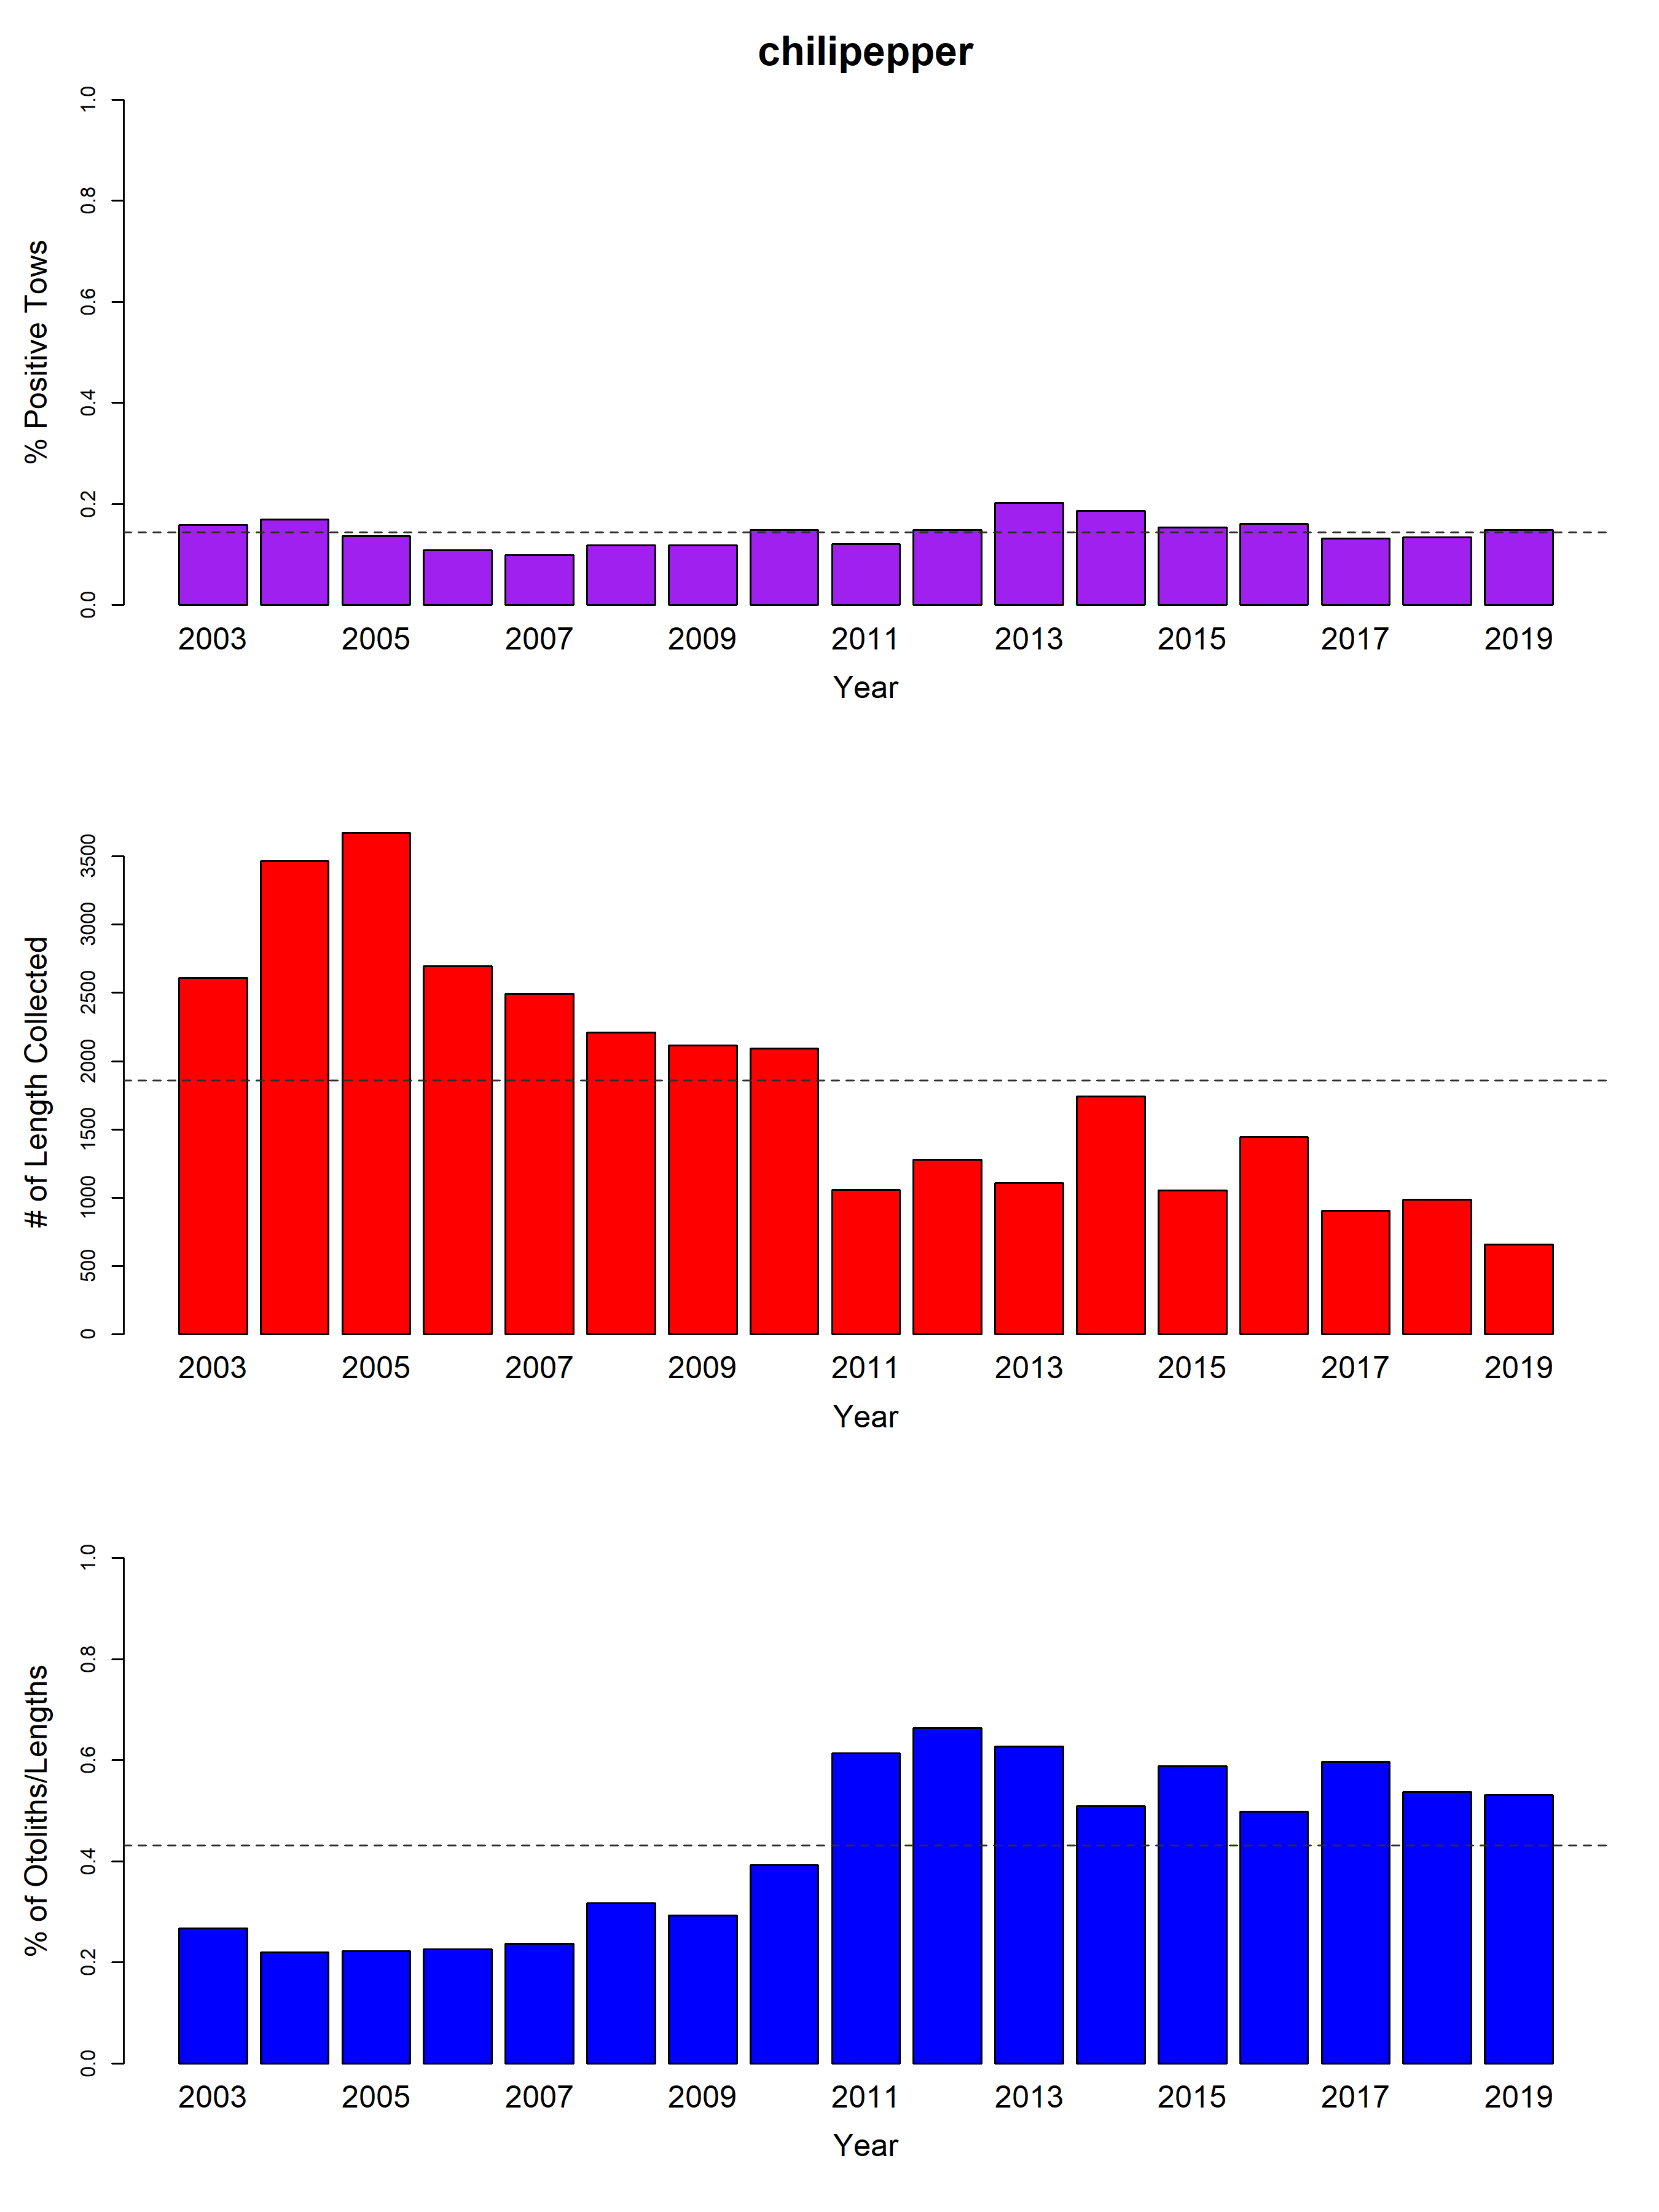
\includegraphics[width=0.6\textwidth,height=\textheight]{C:/Assessments/2020/survey_summary/sum_plots/chilipepper_survey_stats.png}
\FloatBarrier  

\hypertarget{copper-rockfish}{%
\subsection{Copper rockfish}\label{copper-rockfish}}

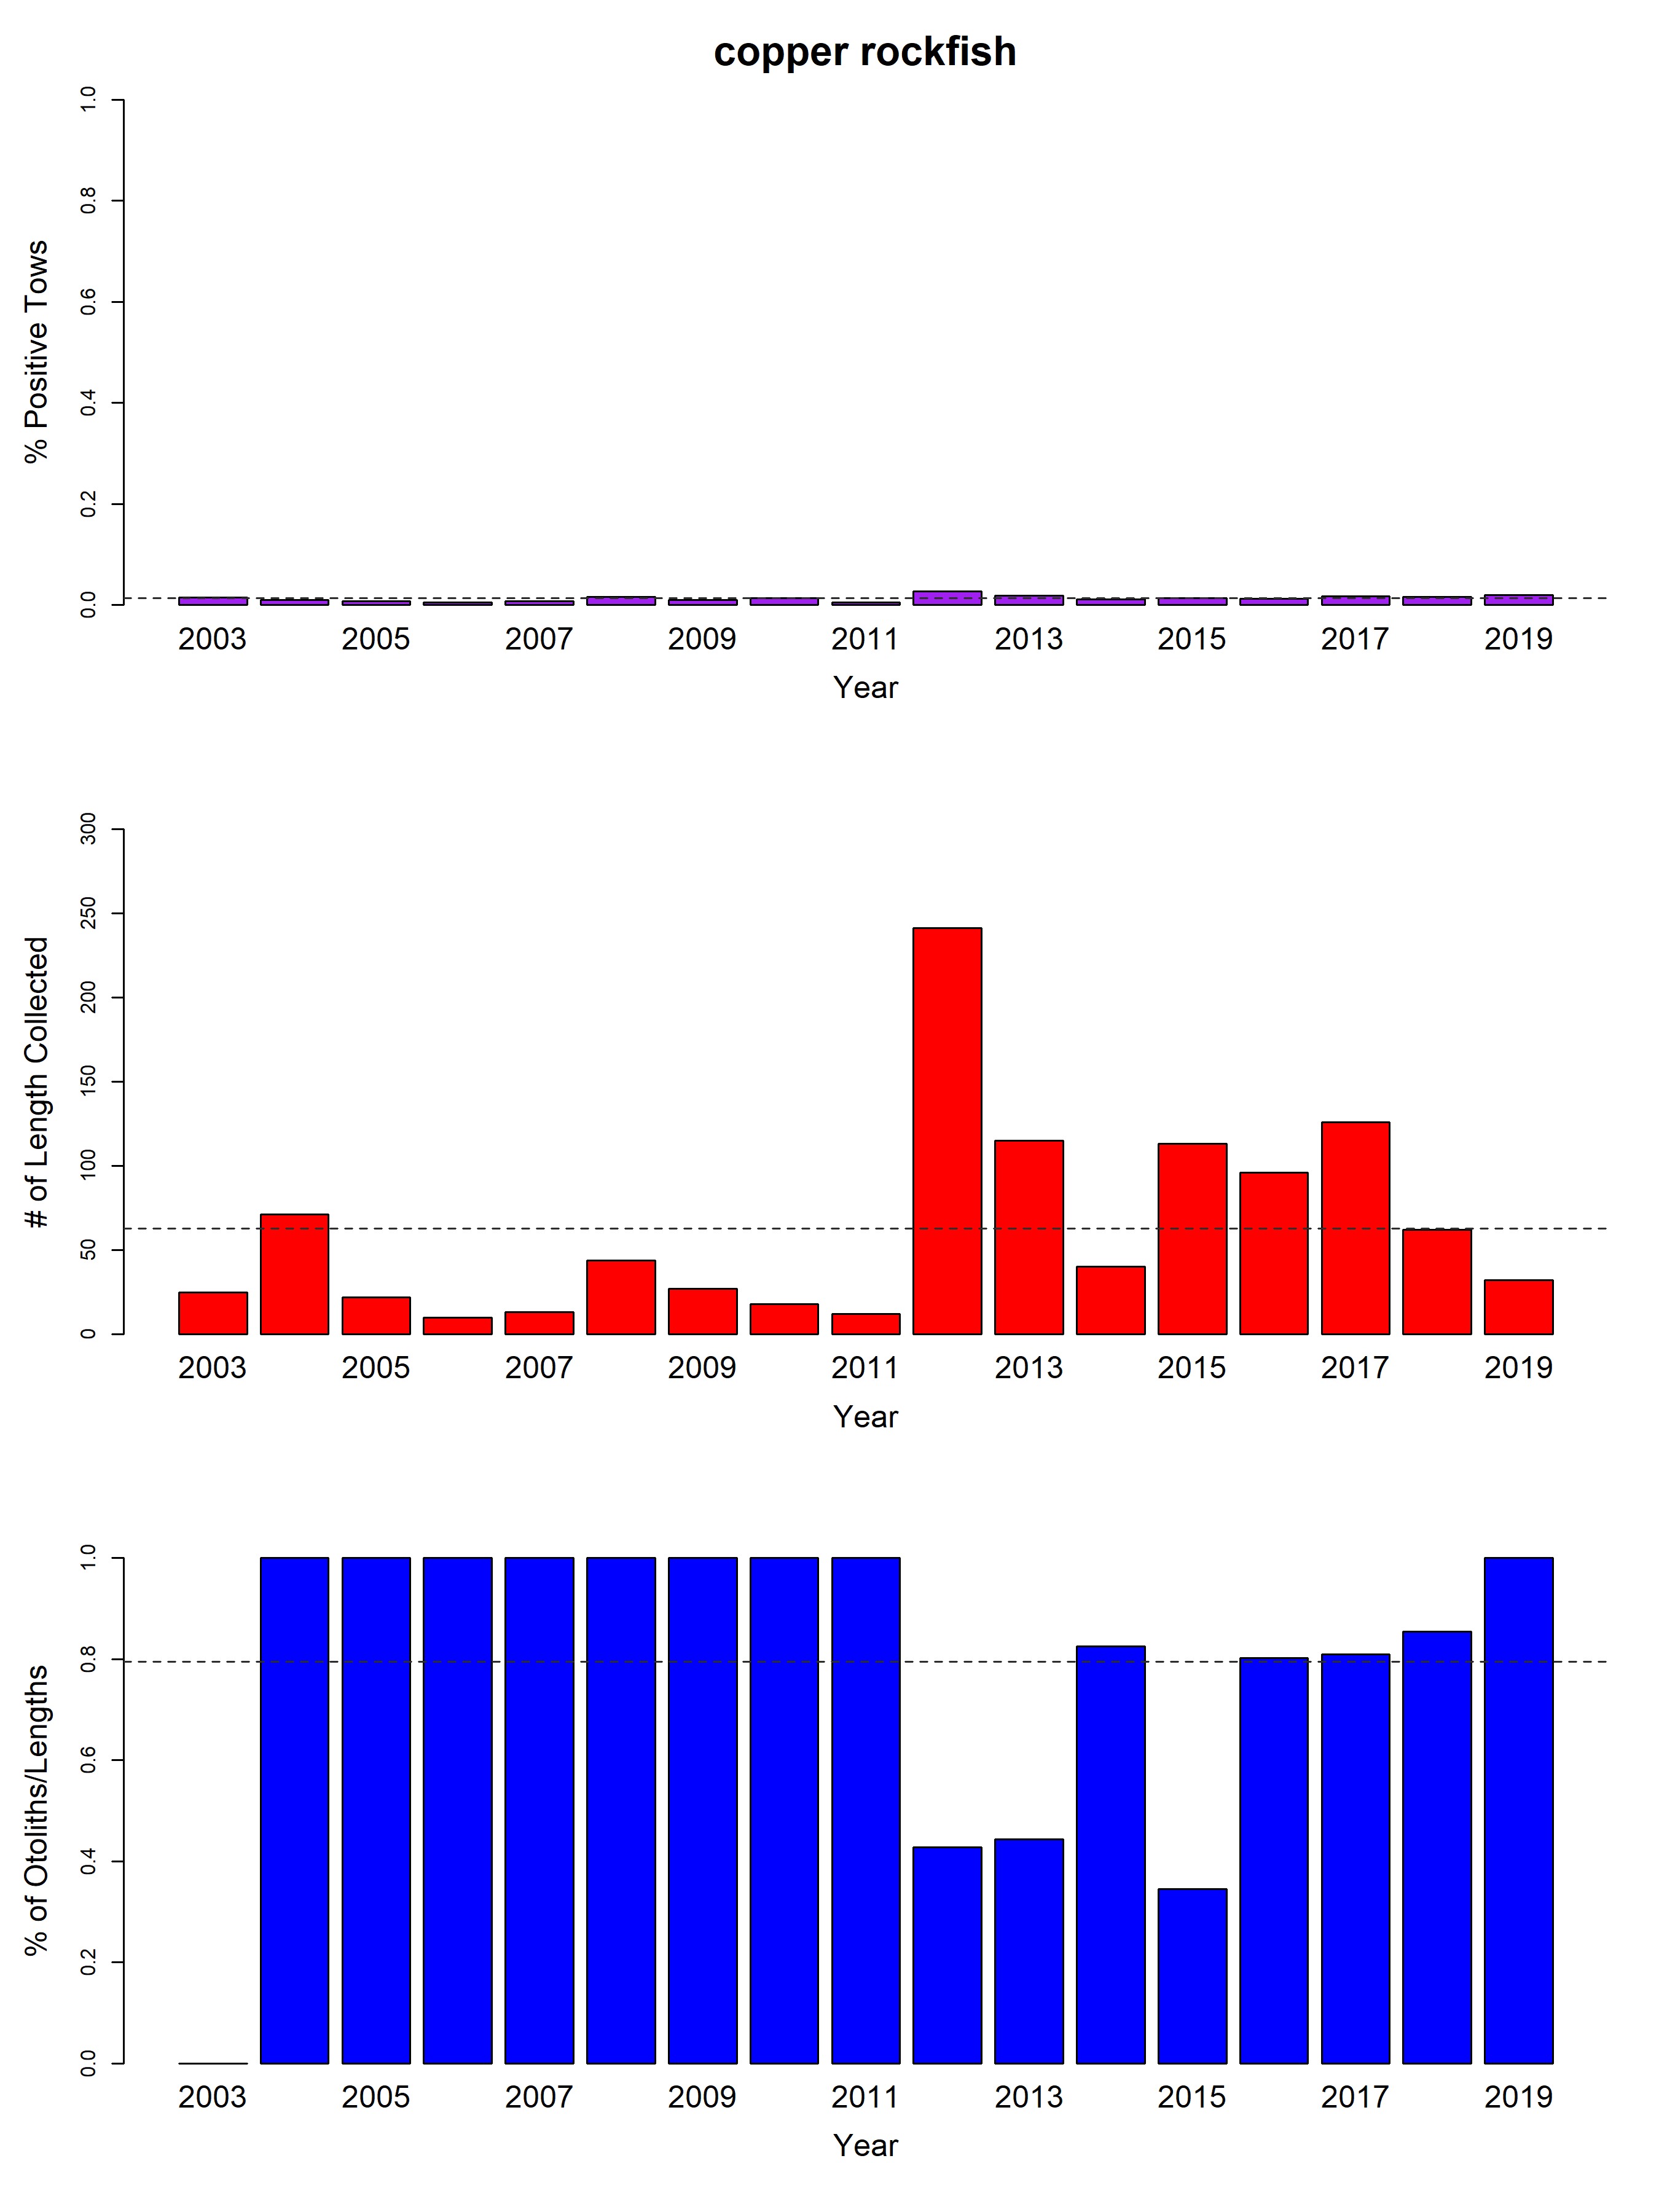
\includegraphics[width=0.6\textwidth,height=\textheight]{C:/Assessments/2020/survey_summary/sum_plots/copper_rockfish_survey_stats.png}
\FloatBarrier  

\hypertarget{cowcod}{%
\subsection{Cowcod}\label{cowcod}}

\FloatBarrier

\hypertarget{darkblotched-rockfish}{%
\subsection{Darkblotched rockfish}\label{darkblotched-rockfish}}

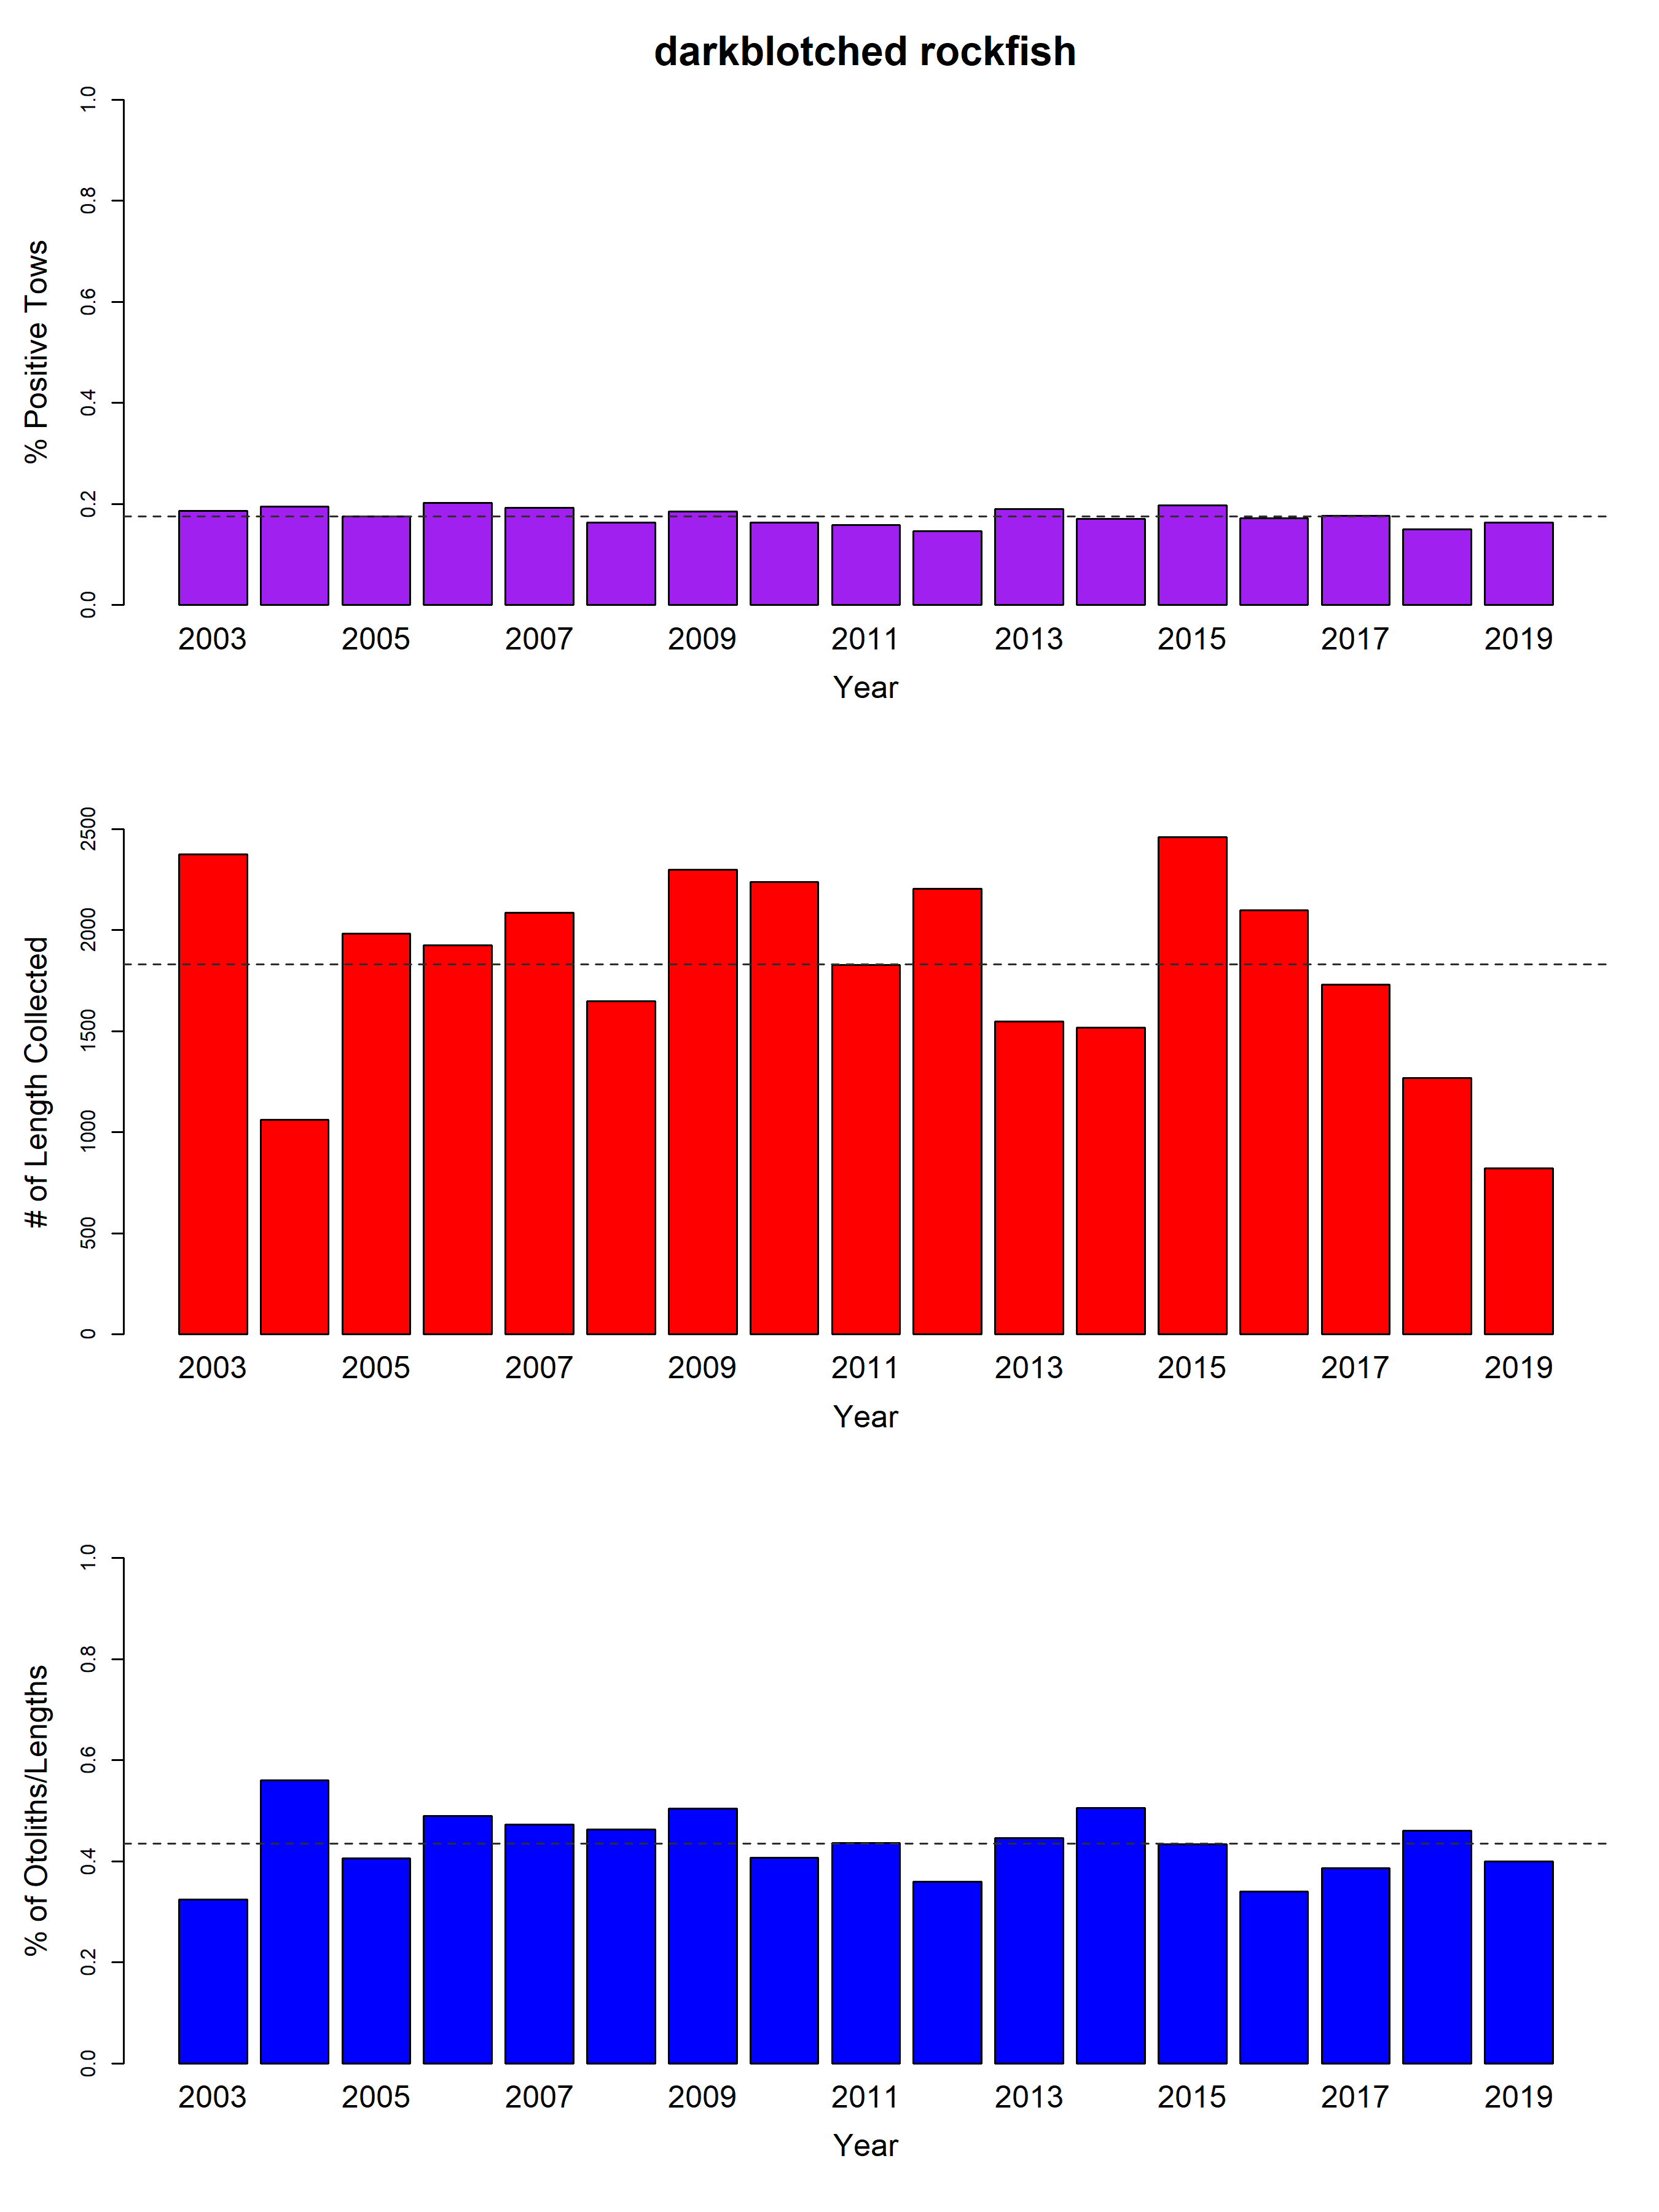
\includegraphics[width=0.6\textwidth,height=\textheight]{C:/Assessments/2020/survey_summary/sum_plots/darkblotched_rockfish_survey_stats.png}
\FloatBarrier  

\hypertarget{dover-sole}{%
\subsection{Dover sole}\label{dover-sole}}

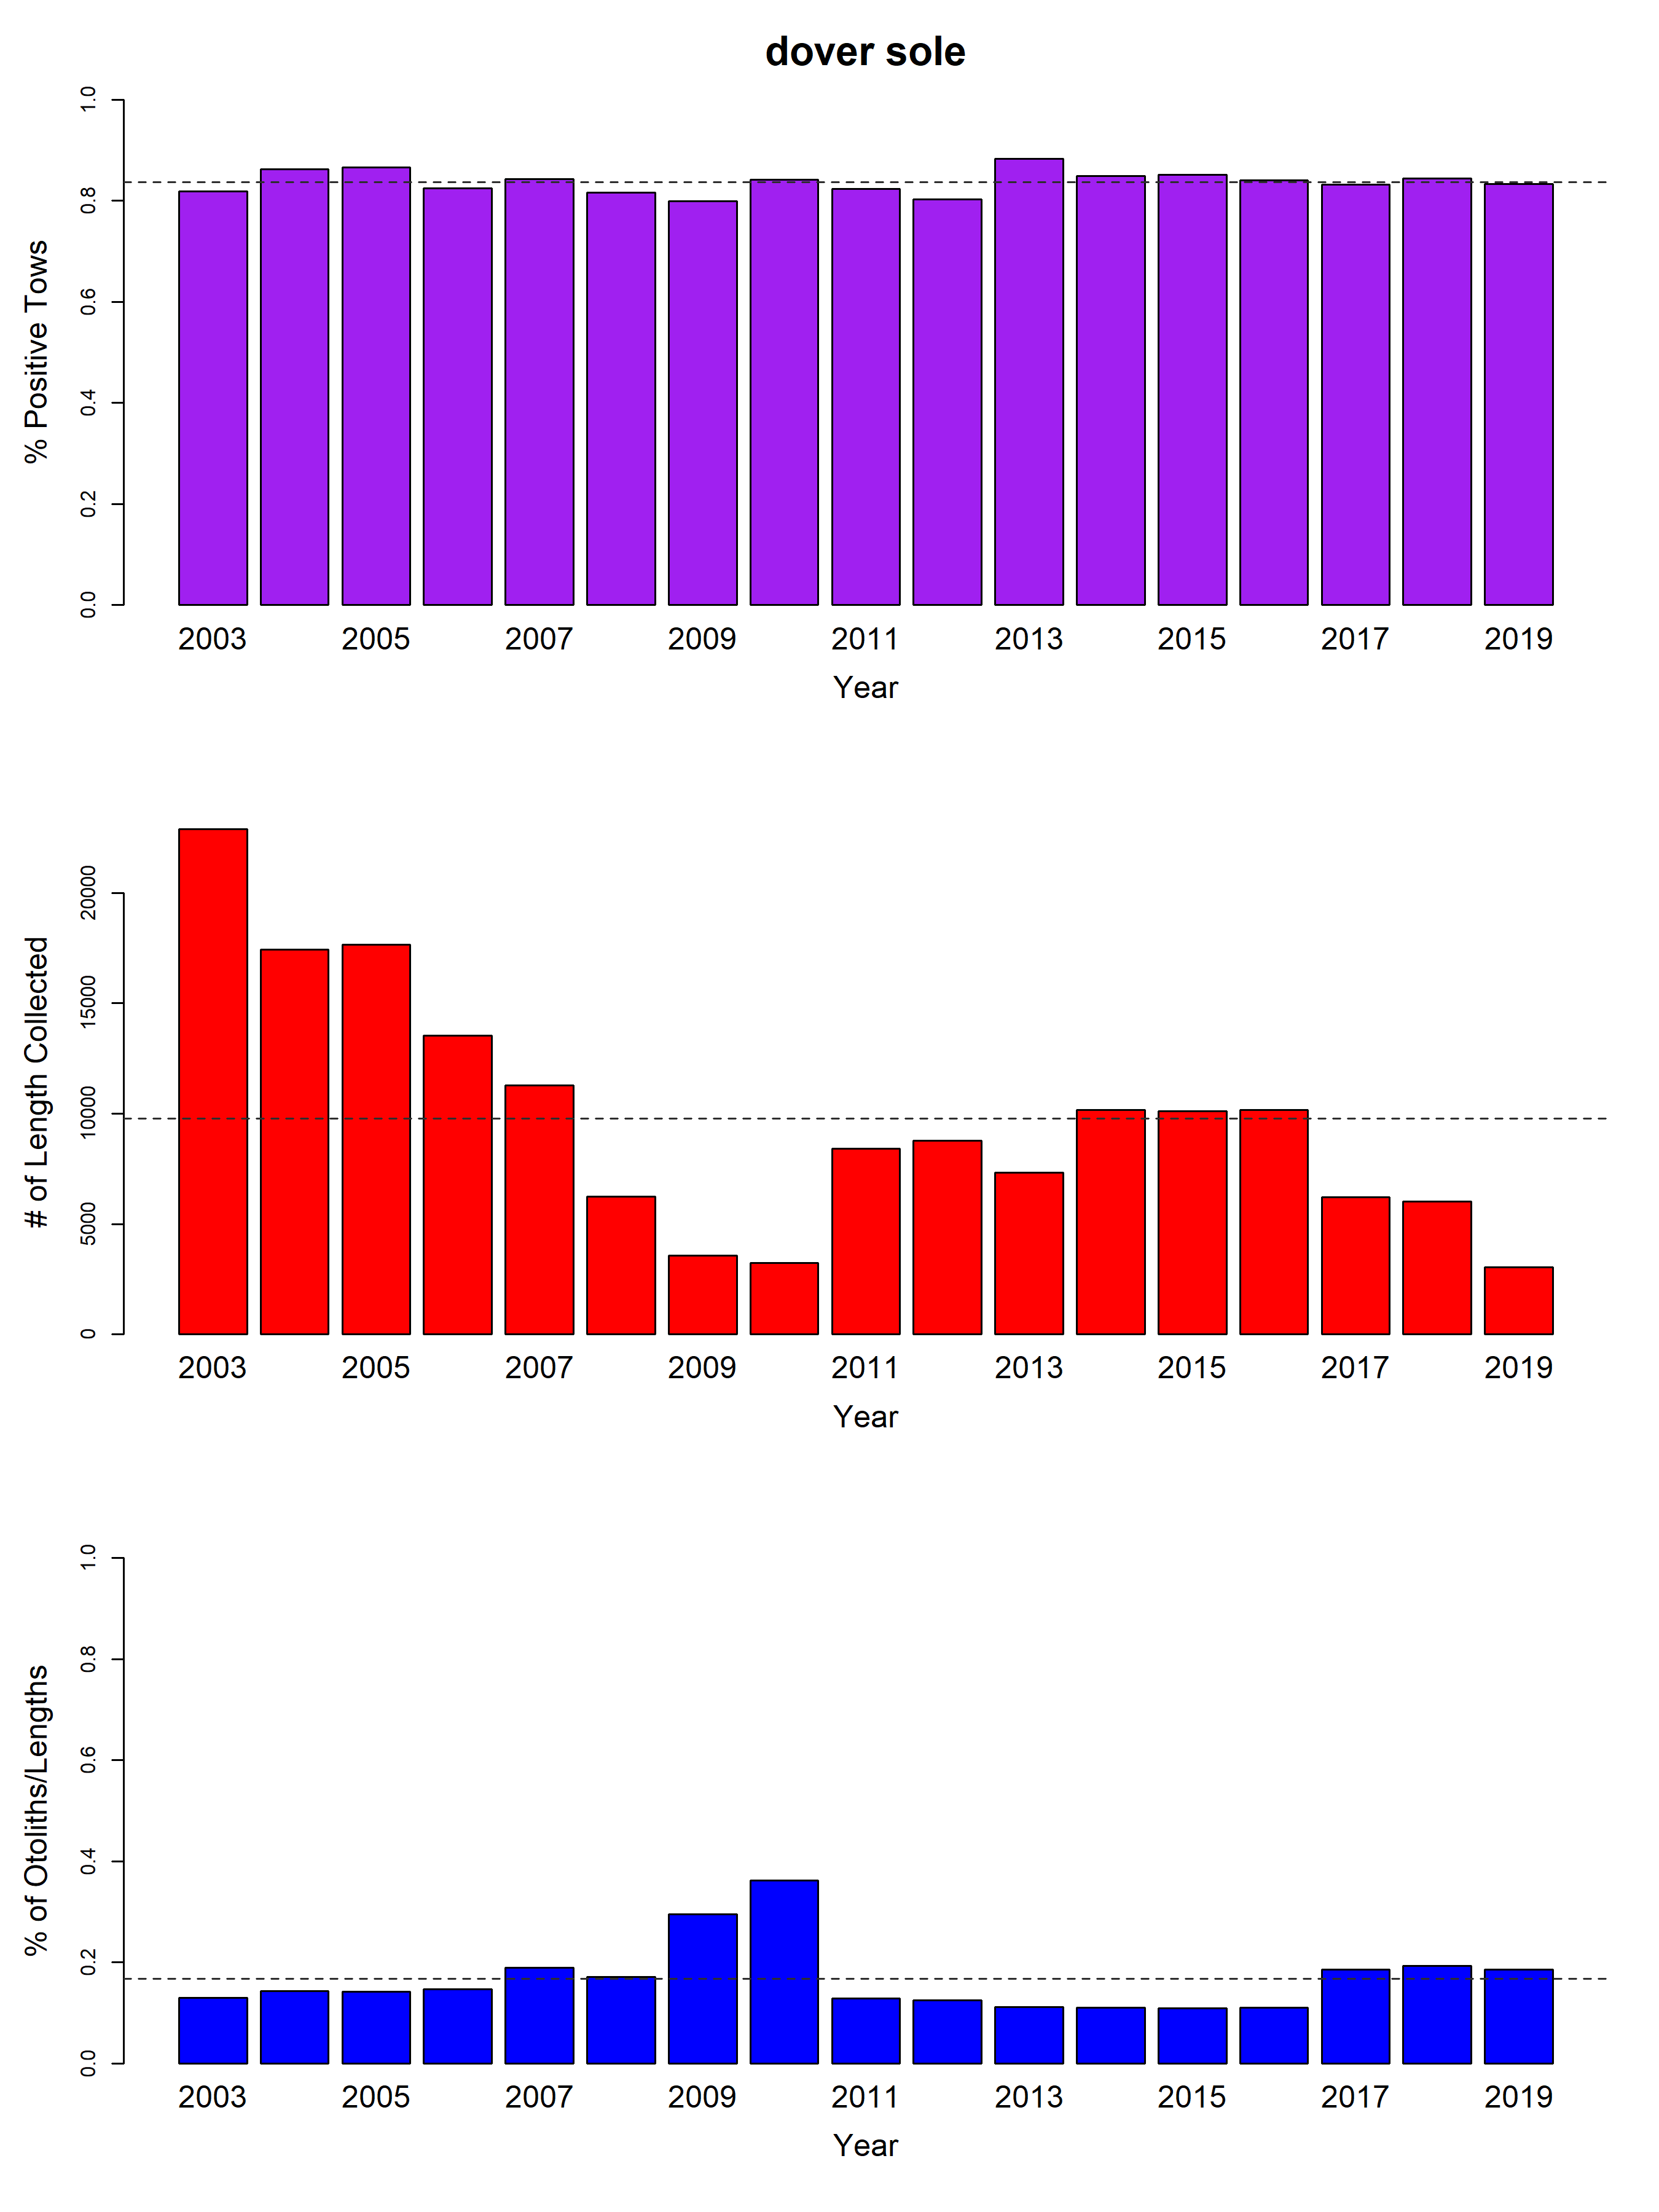
\includegraphics[width=0.6\textwidth,height=\textheight]{C:/Assessments/2020/survey_summary/sum_plots/dover_sole_survey_stats.png}
\FloatBarrier  

\hypertarget{english-sole}{%
\subsection{English sole}\label{english-sole}}

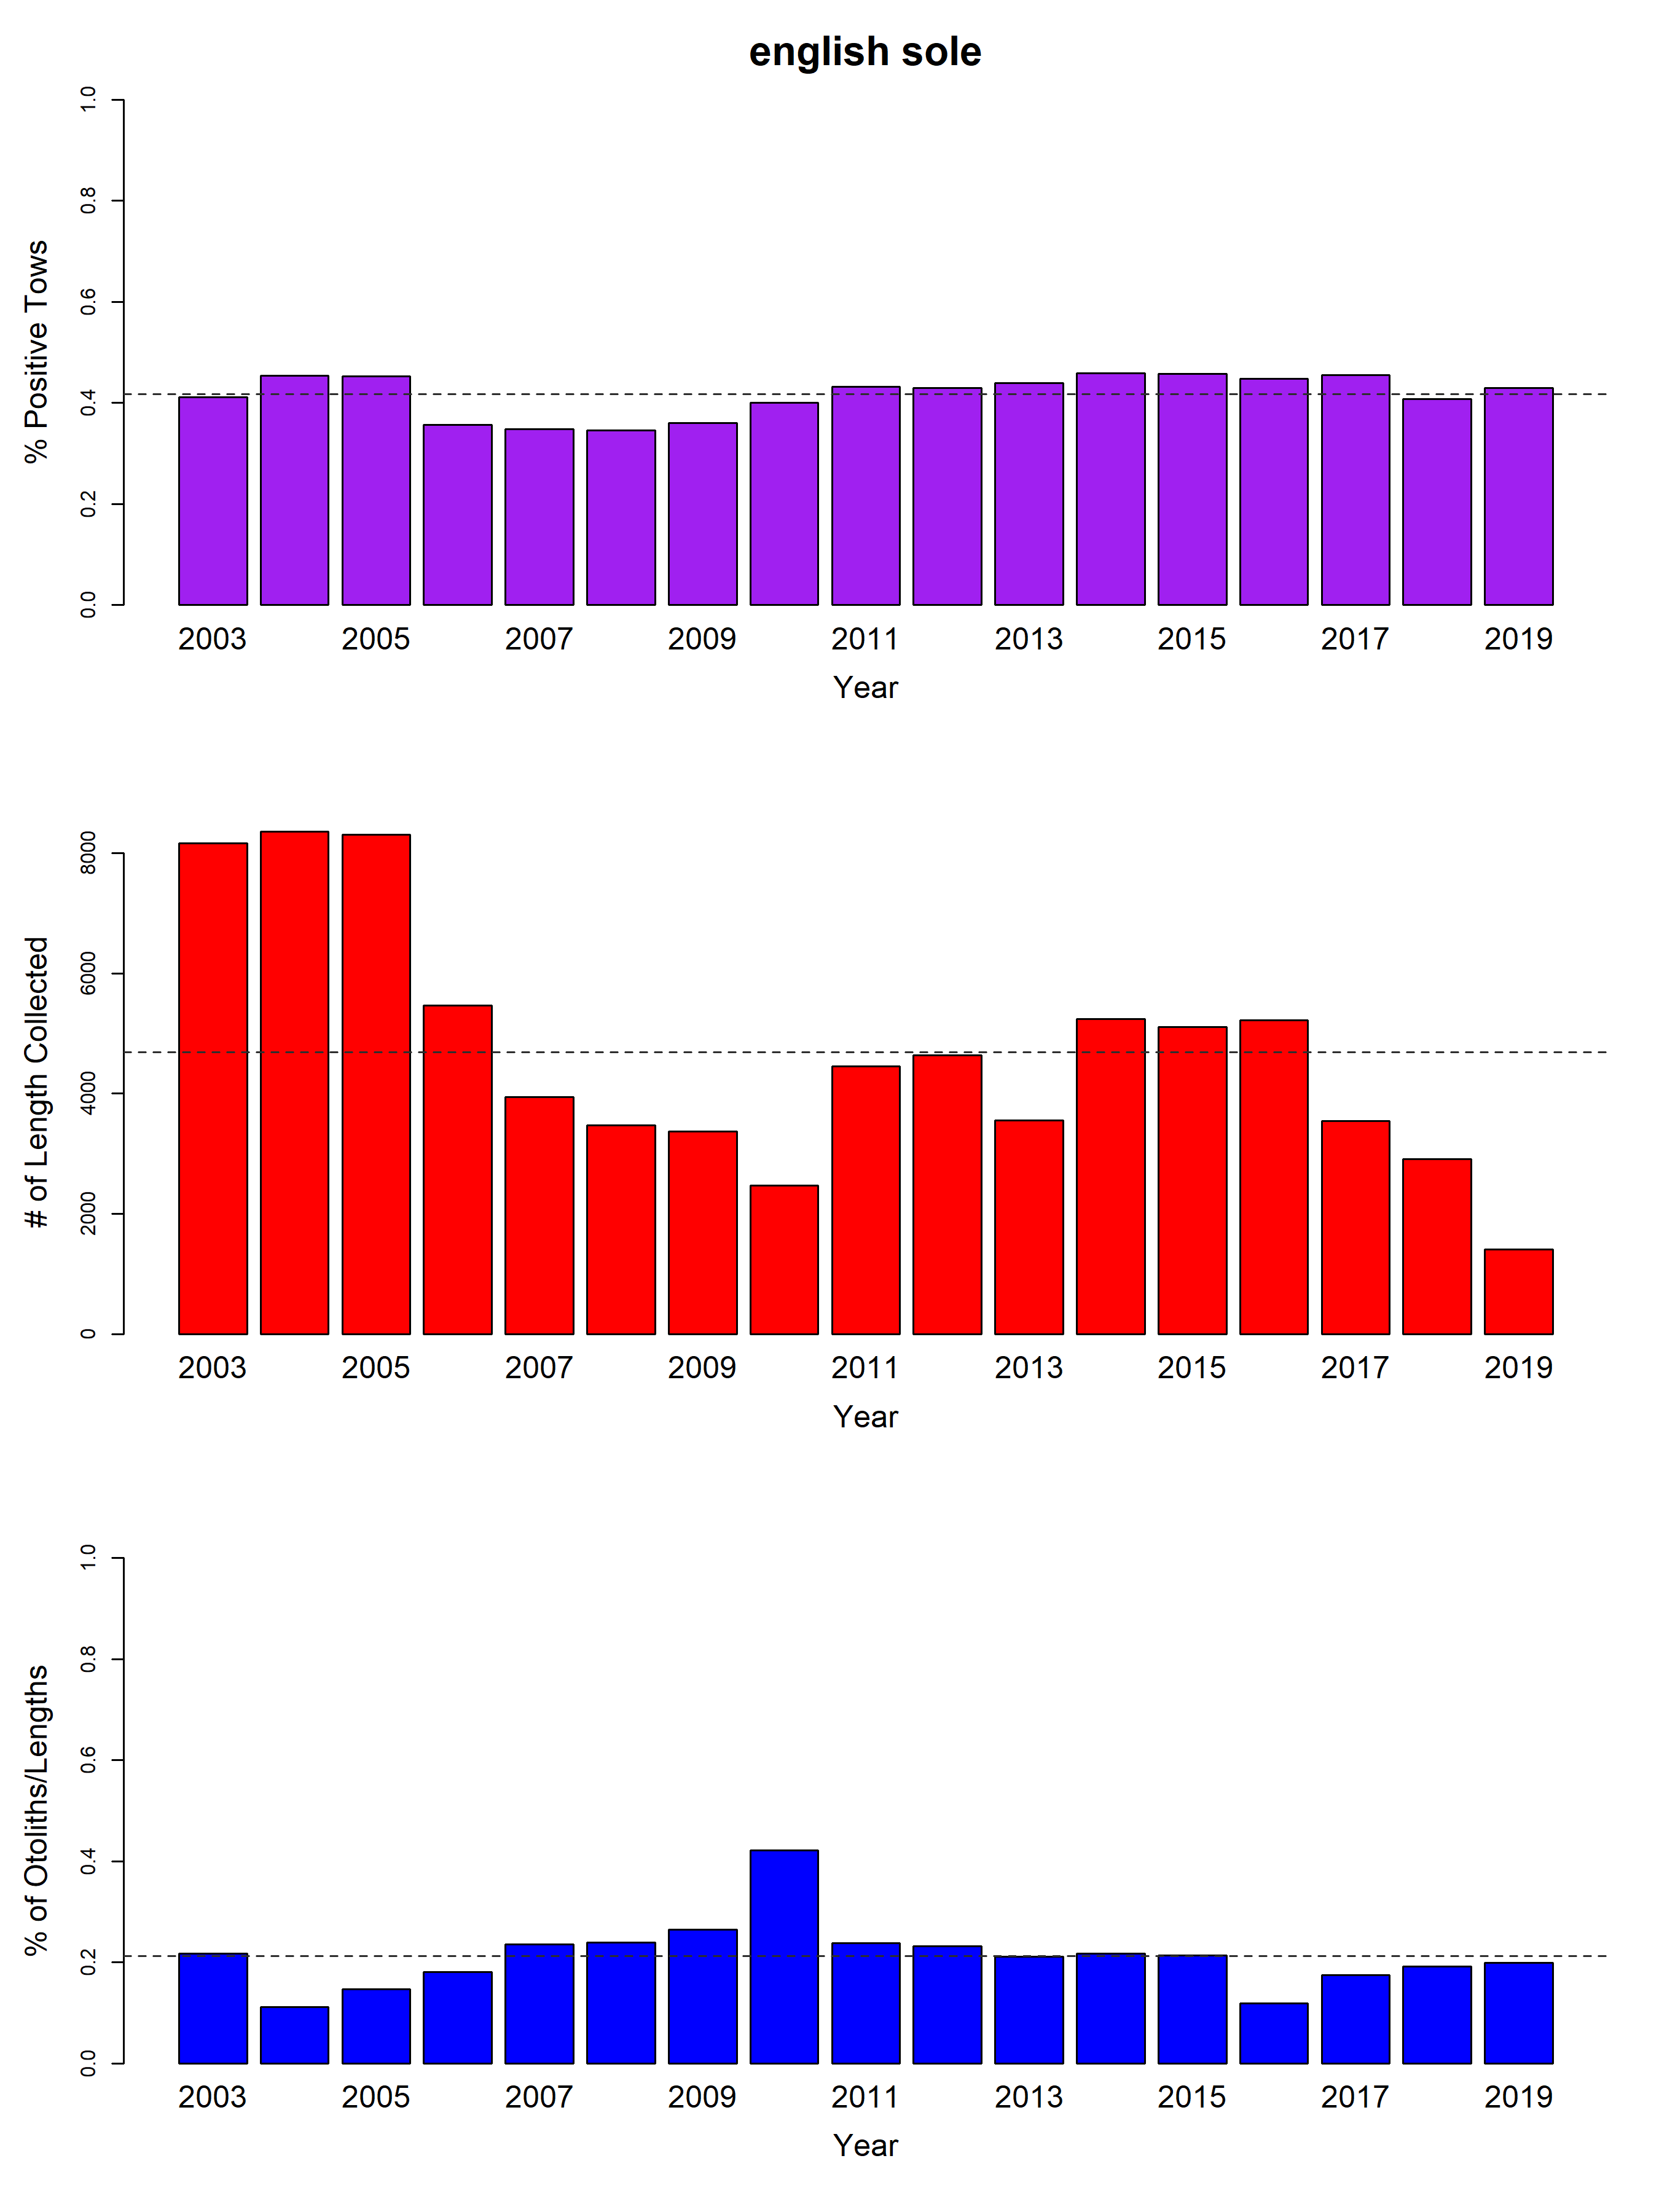
\includegraphics[width=0.6\textwidth,height=\textheight]{C:/Assessments/2020/survey_summary/sum_plots/english_sole_survey_stats.png}
\FloatBarrier  

\hypertarget{flag-rockfish}{%
\subsection{Flag rockfish}\label{flag-rockfish}}

\FloatBarrier

\hypertarget{flathead-sole}{%
\subsection{Flathead sole}\label{flathead-sole}}

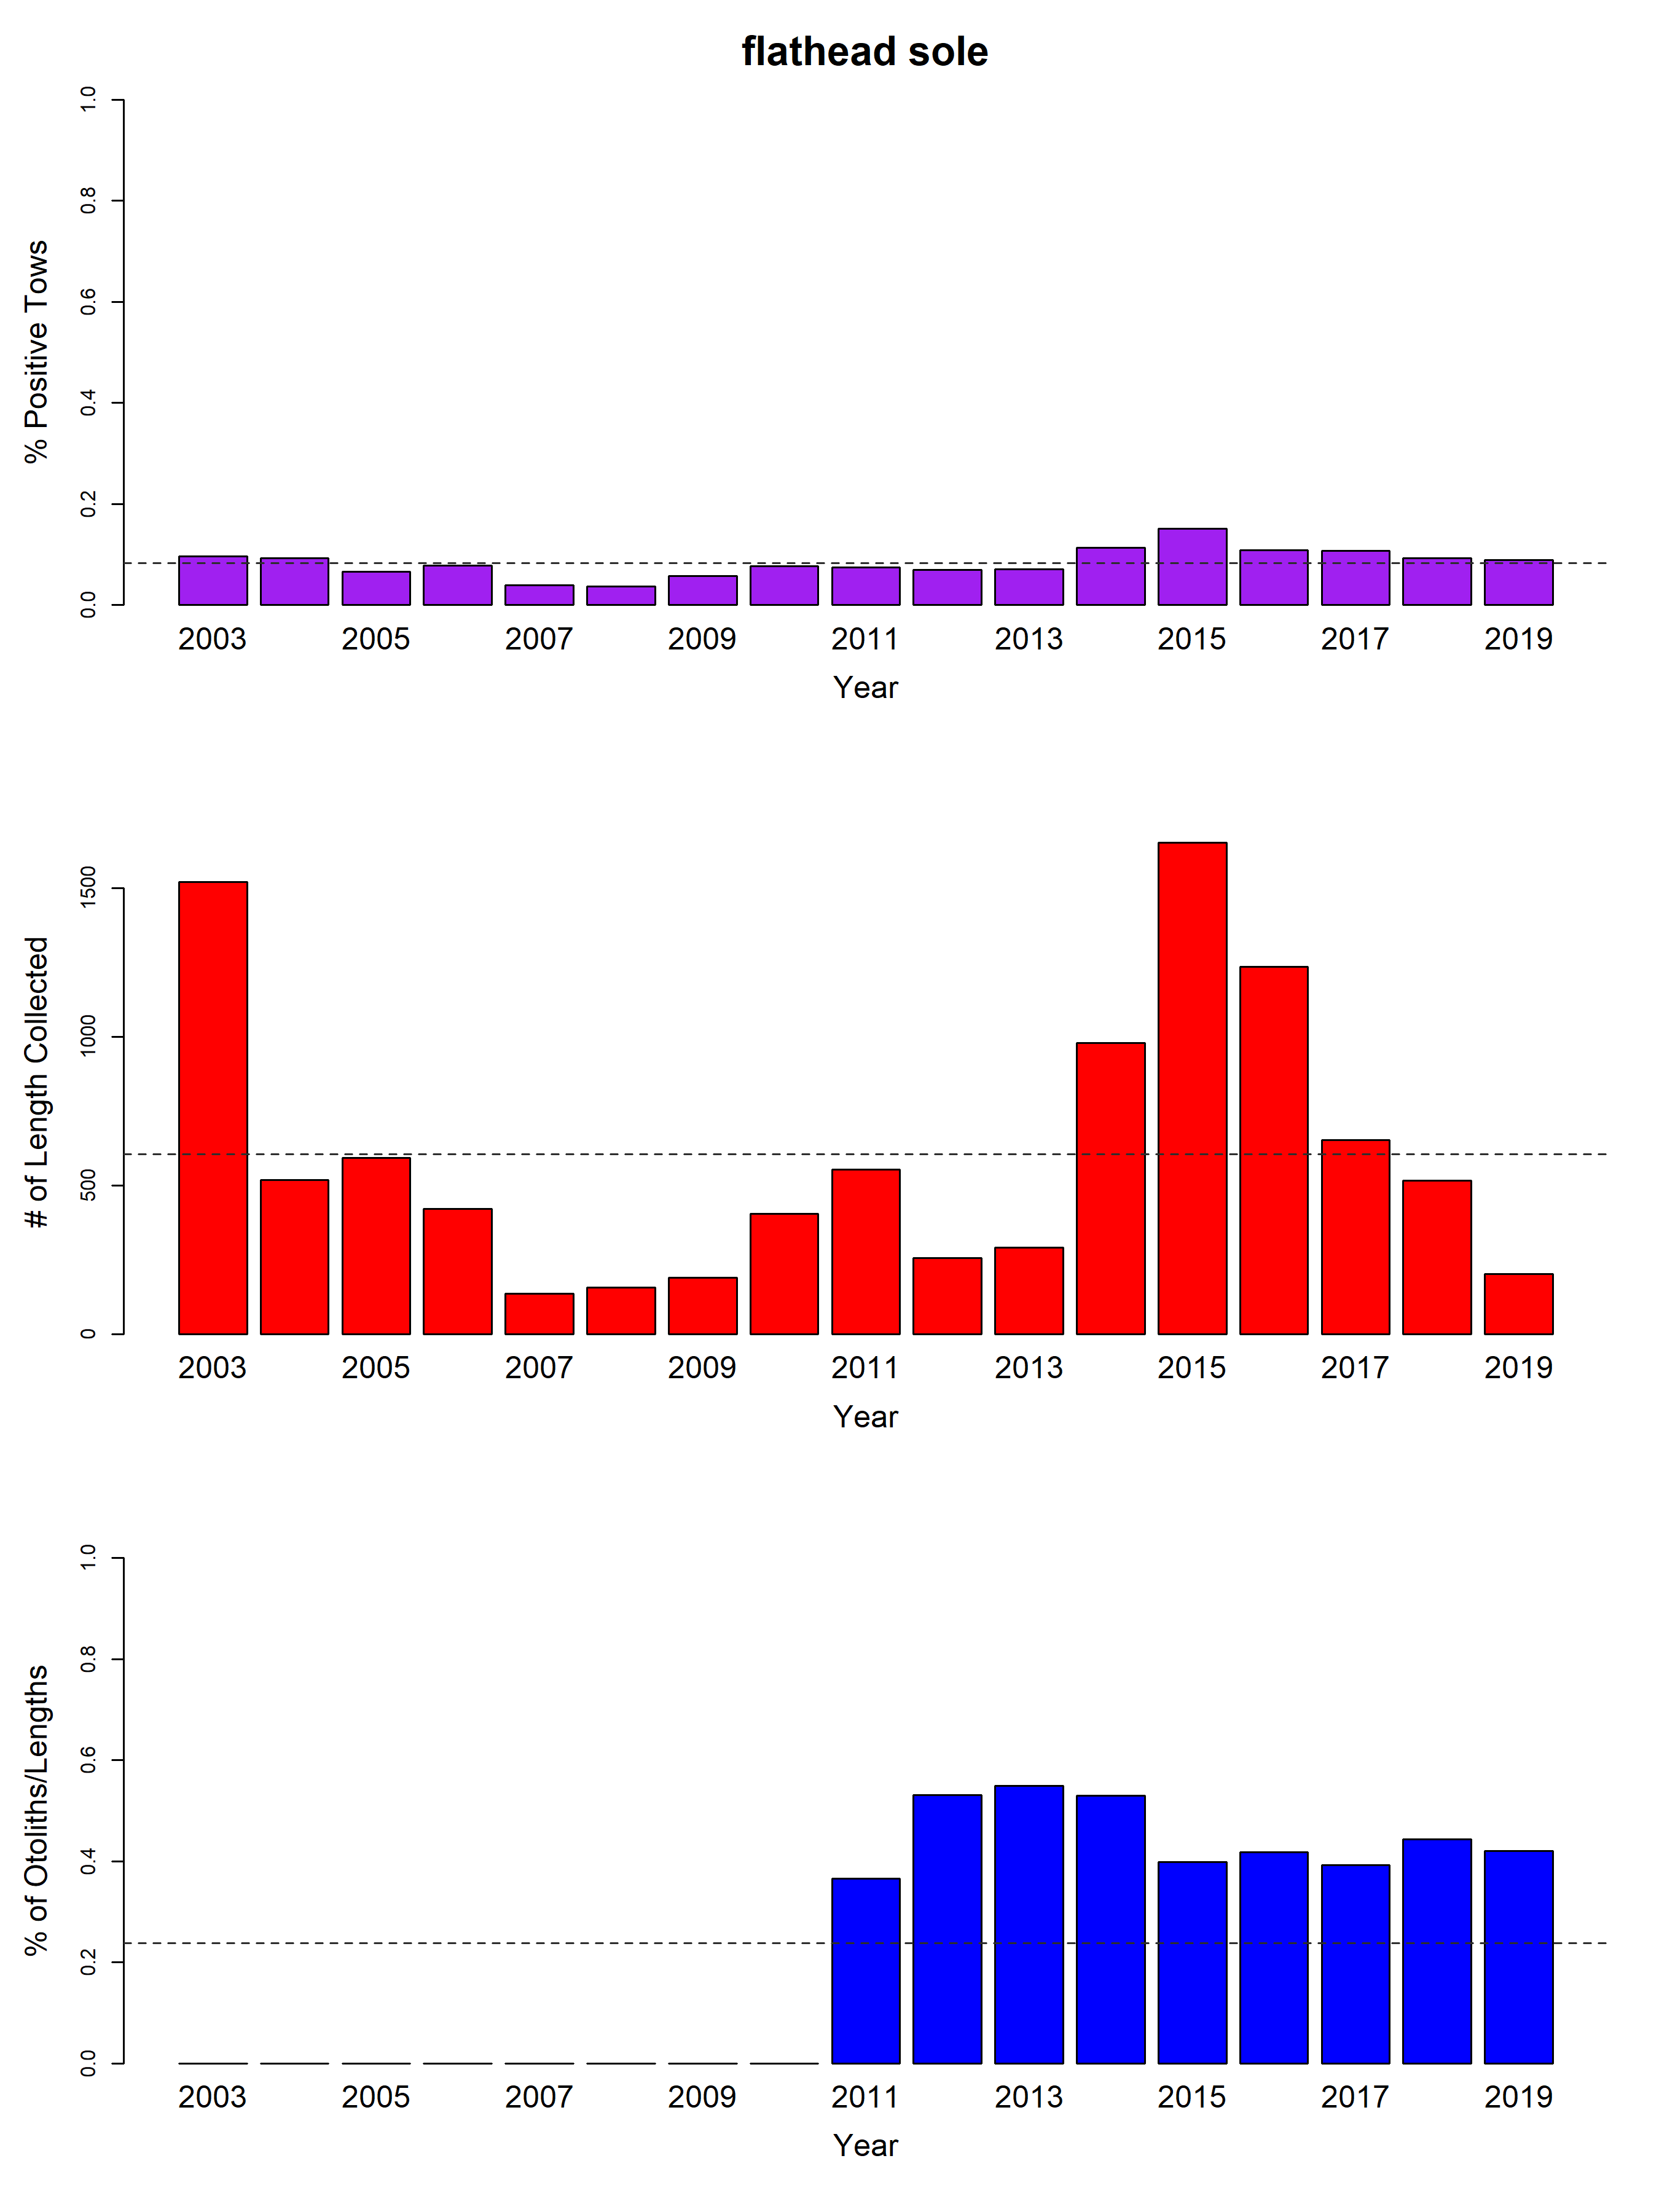
\includegraphics[width=0.6\textwidth,height=\textheight]{C:/Assessments/2020/survey_summary/sum_plots/flathead_sole_survey_stats.png}
\FloatBarrier  

\hypertarget{greenblotched-rockfish}{%
\subsection{Greenblotched rockfish}\label{greenblotched-rockfish}}

\FloatBarrier

\hypertarget{greenspotted-rockfish}{%
\subsection{Greenspotted rockfish}\label{greenspotted-rockfish}}

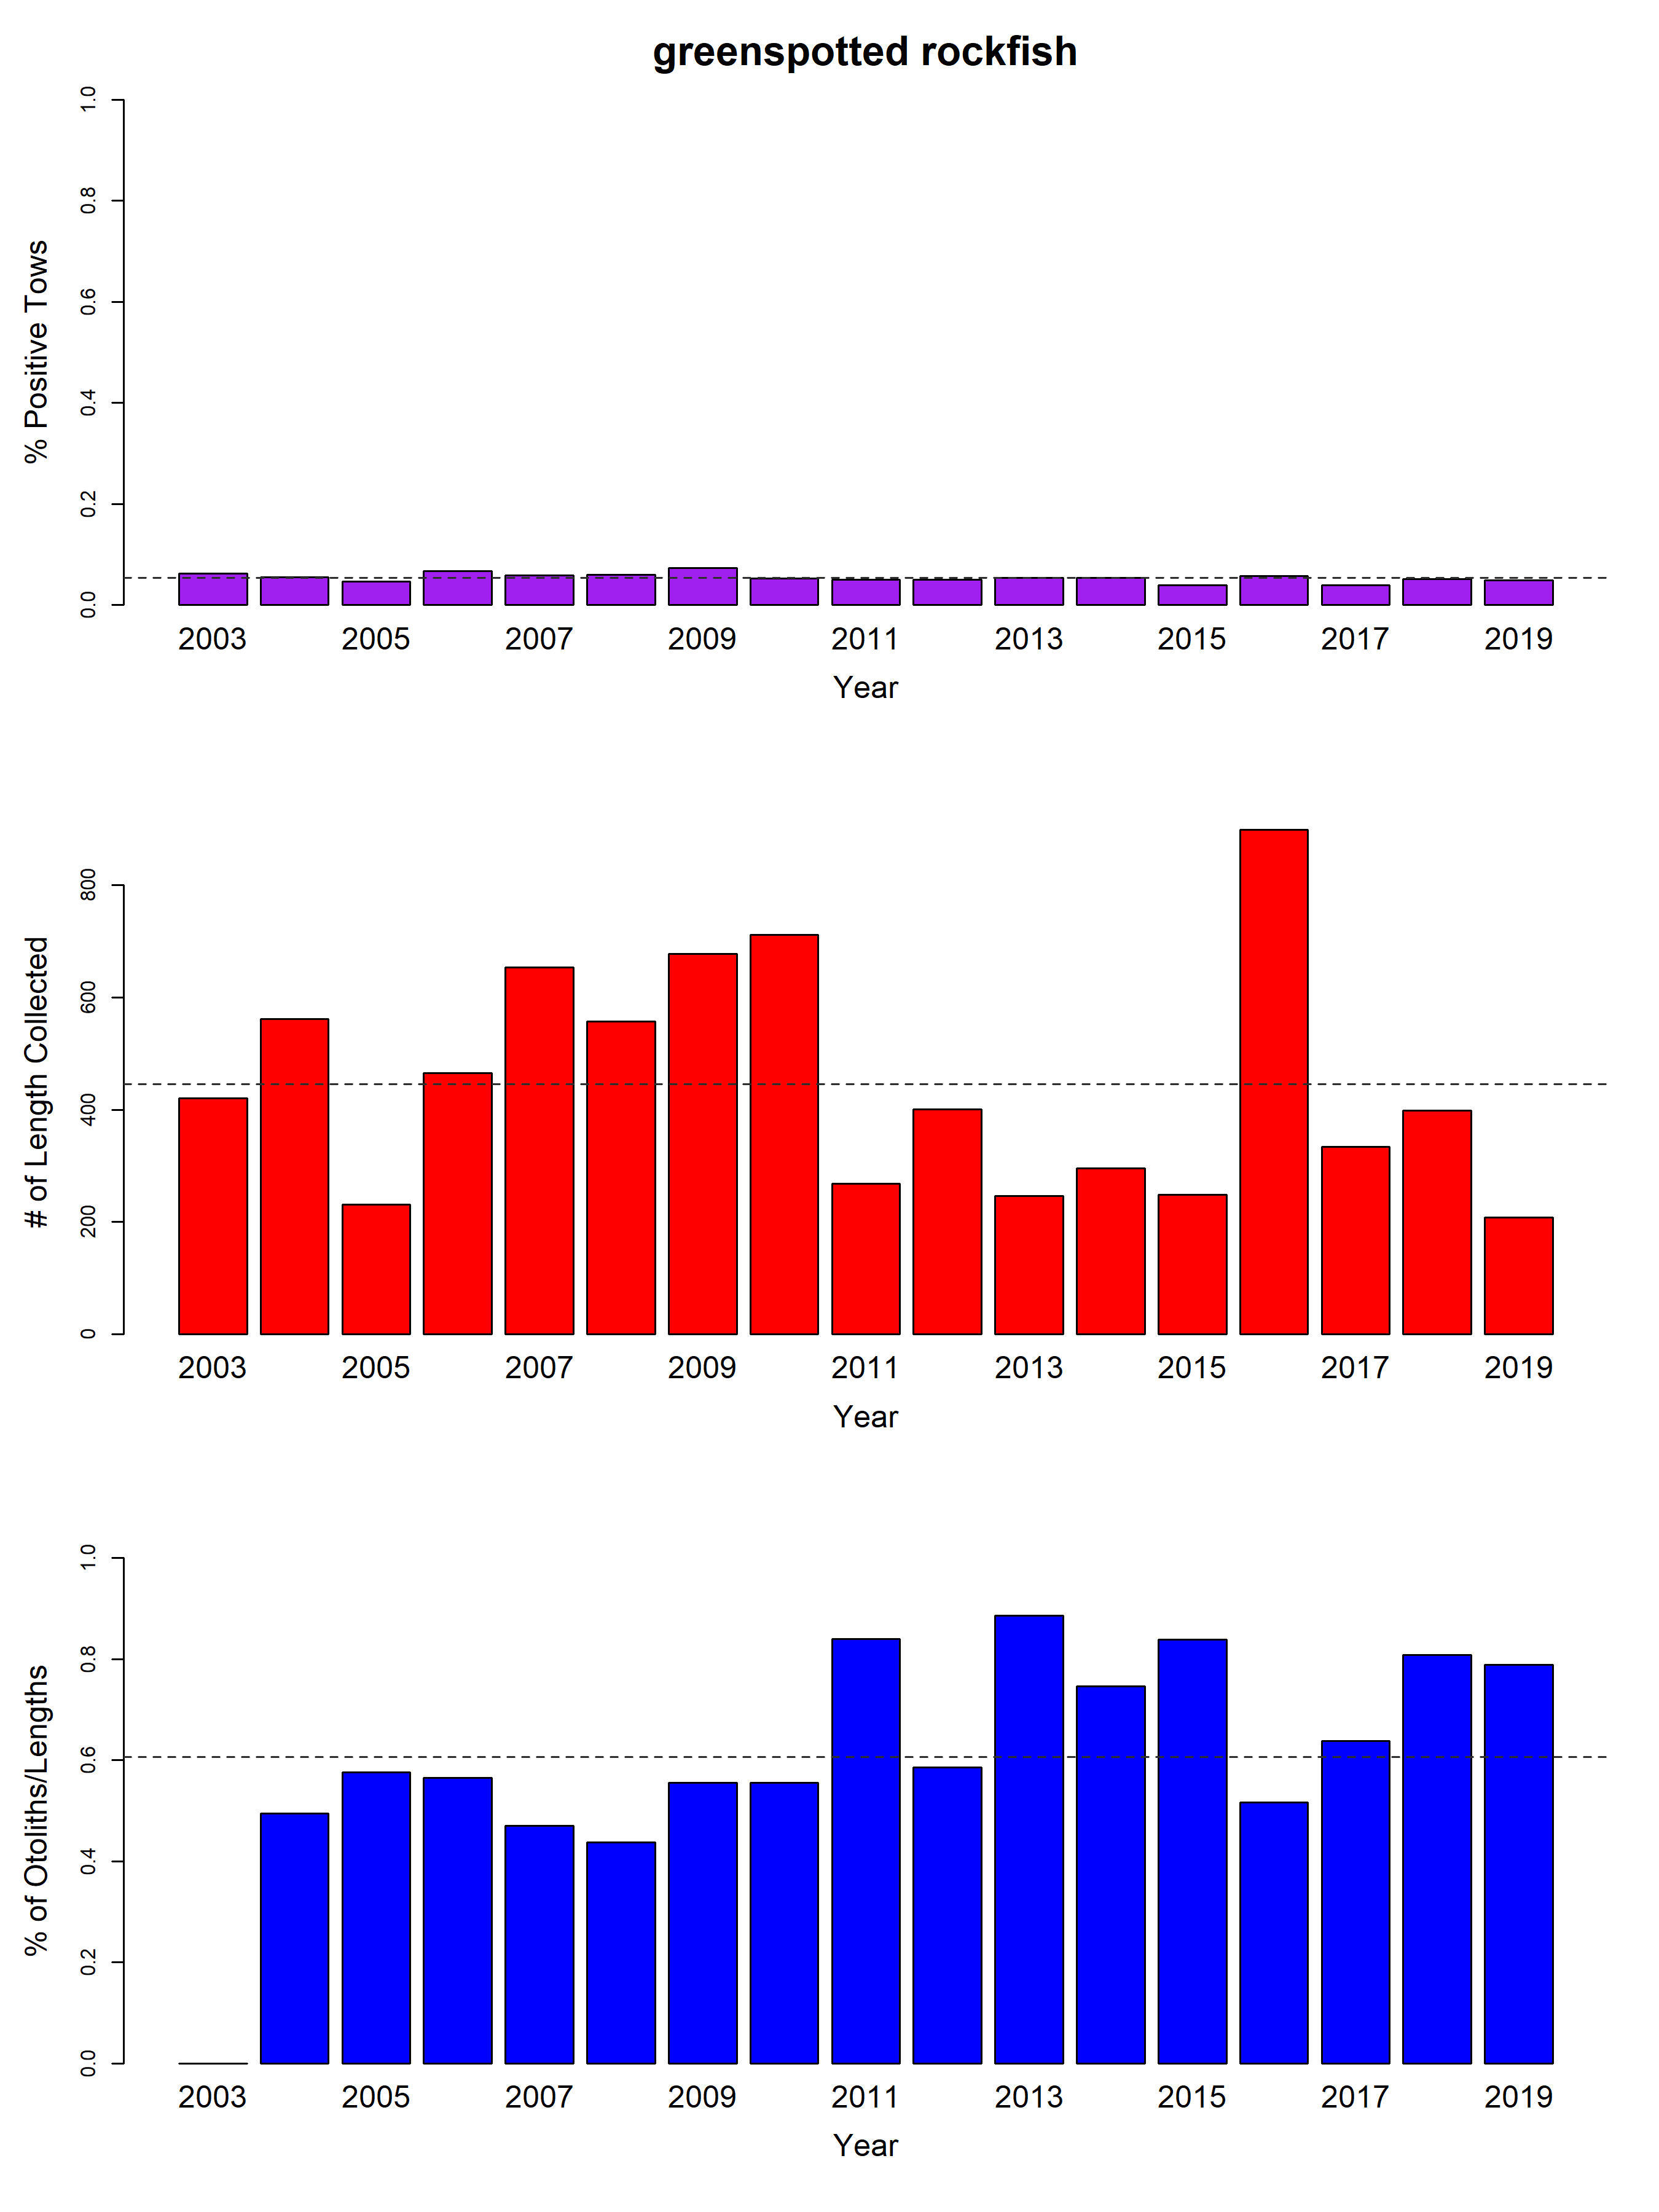
\includegraphics[width=0.6\textwidth,height=\textheight]{C:/Assessments/2020/survey_summary/sum_plots/greenspotted_rockfish_survey_stats.png}
\FloatBarrier  

\hypertarget{greenstriped-rockfish}{%
\subsection{Greenstriped rockfish}\label{greenstriped-rockfish}}

\includegraphics[width=0.6\textwidth,height=\textheight]{C:/Assessments/2020/survey_summary/sum_plots/greenstriped_rockfish_survey_stats.png}
\FloatBarrier  

\hypertarget{halfbanded-rockfish}{%
\subsection{Halfbanded rockfish}\label{halfbanded-rockfish}}

\FloatBarrier

\hypertarget{honeycomb-rockfish}{%
\subsection{Honeycomb rockfish}\label{honeycomb-rockfish}}

\FloatBarrier

\hypertarget{lingcod}{%
\subsection{Lingcod}\label{lingcod}}

\includegraphics[width=0.6\textwidth,height=\textheight]{C:/Assessments/2020/survey_summary/sum_plots/lingcod_survey_stats.png}
\FloatBarrier  

\hypertarget{longnose-skate}{%
\subsection{Longnose skate}\label{longnose-skate}}

\includegraphics[width=0.6\textwidth,height=\textheight]{C:/Assessments/2020/survey_summary/sum_plots/longnose_skate_survey_stats.png}
\FloatBarrier  

\hypertarget{longspine-thornyhead}{%
\subsection{Longspine thornyhead}\label{longspine-thornyhead}}

\includegraphics[width=0.6\textwidth,height=\textheight]{C:/Assessments/2020/survey_summary/sum_plots/longspine_thornyhead_survey_stats.png}
\FloatBarrier  

\hypertarget{olive-rockfish}{%
\subsection{Olive rockfish}\label{olive-rockfish}}

\FloatBarrier

\hypertarget{pacific-cod}{%
\subsection{Pacific cod}\label{pacific-cod}}

\includegraphics[width=0.6\textwidth,height=\textheight]{C:/Assessments/2020/survey_summary/sum_plots/pacific_cod_survey_stats.png}
\FloatBarrier  

\hypertarget{pacific-ocean-perch}{%
\subsection{Pacific ocean perch}\label{pacific-ocean-perch}}

\includegraphics[width=0.6\textwidth,height=\textheight]{C:/Assessments/2020/survey_summary/sum_plots/pacific_ocean_perch_survey_stats.png}
\FloatBarrier  

\hypertarget{pacific-sanddab}{%
\subsection{Pacific sanddab}\label{pacific-sanddab}}

\includegraphics[width=0.6\textwidth,height=\textheight]{C:/Assessments/2020/survey_summary/sum_plots/pacific_sanddab_survey_stats.png}
\FloatBarrier  

\hypertarget{pacific-spiny-dogfish}{%
\subsection{Pacific spiny dogfish}\label{pacific-spiny-dogfish}}

\includegraphics[width=0.6\textwidth,height=\textheight]{C:/Assessments/2020/survey_summary/sum_plots/pacific_spiny_dogfish_survey_stats.png}
\FloatBarrier  

\hypertarget{petrale-sole}{%
\subsection{Petrale sole}\label{petrale-sole}}

\includegraphics[width=0.6\textwidth,height=\textheight]{C:/Assessments/2020/survey_summary/sum_plots/petrale_sole_survey_stats.png}
\FloatBarrier  

\hypertarget{redbanded-rockfish}{%
\subsection{Redbanded rockfish}\label{redbanded-rockfish}}

\includegraphics[width=0.6\textwidth,height=\textheight]{C:/Assessments/2020/survey_summary/sum_plots/redbanded_rockfish_survey_stats.png}
\FloatBarrier  

\hypertarget{rex-sole}{%
\subsection{Rex sole}\label{rex-sole}}

\includegraphics[width=0.6\textwidth,height=\textheight]{C:/Assessments/2020/survey_summary/sum_plots/rex_sole_survey_stats.png}
\FloatBarrier  

\hypertarget{rosy-rockfish}{%
\subsection{Rosy rockfish}\label{rosy-rockfish}}

\FloatBarrier

\hypertarget{rougheye-rockfish}{%
\subsection{Rougheye rockfish}\label{rougheye-rockfish}}

\includegraphics[width=0.6\textwidth,height=\textheight]{C:/Assessments/2020/survey_summary/sum_plots/rougheye_rockfish_survey_stats.png}
\FloatBarrier  

\hypertarget{sablefish}{%
\subsection{Sablefish}\label{sablefish}}

\includegraphics[width=0.6\textwidth,height=\textheight]{C:/Assessments/2020/survey_summary/sum_plots/sablefish_survey_stats.png}
\FloatBarrier  

\hypertarget{sharpchin-rockfish}{%
\subsection{Sharpchin rockfish}\label{sharpchin-rockfish}}

\includegraphics[width=0.6\textwidth,height=\textheight]{C:/Assessments/2020/survey_summary/sum_plots/sharpchin_rockfish_survey_stats.png}
\FloatBarrier  

\hypertarget{shortbelly-rockfish}{%
\subsection{Shortbelly rockfish}\label{shortbelly-rockfish}}

\includegraphics[width=0.6\textwidth,height=\textheight]{C:/Assessments/2020/survey_summary/sum_plots/shortbelly_rockfish_survey_stats.png}
\FloatBarrier  

\hypertarget{shortspine-thornyhead}{%
\subsection{Shortspine thornyhead}\label{shortspine-thornyhead}}

\includegraphics[width=0.6\textwidth,height=\textheight]{C:/Assessments/2020/survey_summary/sum_plots/shortspine_thornyhead_survey_stats.png}
\FloatBarrier  

\hypertarget{speckled-rockfish}{%
\subsection{Speckled rockfish}\label{speckled-rockfish}}

\FloatBarrier

\hypertarget{splitnose-rockfish}{%
\subsection{Splitnose rockfish}\label{splitnose-rockfish}}

\includegraphics[width=0.6\textwidth,height=\textheight]{C:/Assessments/2020/survey_summary/sum_plots/splitnose_rockfish_survey_stats.png}
\FloatBarrier  

\hypertarget{squarespot-rockfish}{%
\subsection{Squarespot rockfish}\label{squarespot-rockfish}}

\FloatBarrier

\hypertarget{starry-rockfish}{%
\subsection{Starry rockfish}\label{starry-rockfish}}

\FloatBarrier

\hypertarget{swordspine-rockfish}{%
\subsection{Swordspine rockfish}\label{swordspine-rockfish}}

\FloatBarrier

\hypertarget{vermilion-rockfish}{%
\subsection{Vermilion rockfish}\label{vermilion-rockfish}}

\FloatBarrier

\hypertarget{widow-rockfish}{%
\subsection{Widow rockfish}\label{widow-rockfish}}

\includegraphics[width=0.6\textwidth,height=\textheight]{C:/Assessments/2020/survey_summary/sum_plots/widow_rockfish_survey_stats.png}
\FloatBarrier  

\hypertarget{yelloweye-rockfish}{%
\subsection{Yelloweye rockfish}\label{yelloweye-rockfish}}

\FloatBarrier

\hypertarget{yellowtail-rockfish}{%
\subsection{Yellowtail rockfish}\label{yellowtail-rockfish}}

\includegraphics[width=0.6\textwidth,height=\textheight]{C:/Assessments/2020/survey_summary/sum_plots/yellowtail_rockfish_survey_stats.png}
\FloatBarrier  

\end{document}
